\documentclass[10pt, compress]{beamer}
\usetheme{Rochester}
\usecolortheme{beaver}
\beamertemplatenavigationsymbolsempty

\usepackage{pgfplots}
\usepackage{pgf}
\usepackage{tikz}
\usepackage{graphicx}
\usepackage{subcaption}

\title{Evaluating Compression}
\date{\today}
\author{Lukas Stabe, Arne Struck, Hans Ole Hatzel}


\section{Introduction}
\begin{document}
\maketitle
\begin{frame}{Overview}
    \tableofcontents
\end{frame}


\begin{frame}{Assignment}
    \begin{itemize}
        \item Benchmark different algorithms
        \item on different sets of scientific data
        \item automate benchmarking of whole directory structures
        \item visualize results
        \item assess which algorithms are the best
    \end{itemize}
\end{frame}
\begin{frame}{What is fsbench?}
    \begin{itemize}
        \item FOSS-tool
        \item written in C++
        \item support for multiple threads
        \item comes with a lot of algorithms included
    \end{itemize}
    \vspace{1em}
    Since the tool perfectly fits our usecase we decided to use it.
    The project can be found here:    
    \url{https://chiselapp.com/user/Justin_be_my_guide/repository/fsbench}
\end{frame}
\begin{frame}{How does our benchmark script work?}
    \begin{itemize}
        \item Python 3 script
        \item scans directory structure
        \item launches fsbench distributed on each core
        \item saves the results in a sqlite3 database
    \end{itemize}    
\end{frame}

\begin{frame}{How does our plotting script work?}
    \begin{itemize}
        \item Python 3 script
        \item reads results from database
        \item filters according to given command-line options
        \item prints results in a pretty graph using matplotlib
        \item prints base data as a latex 
    \end{itemize}    
\end{frame}

\section{Procedure}
\begin{frame}{Plan}
    \begin{itemize}
        \item choose datasets
        \item write script
        \item execute script
        \item have beautiful data
        \item decide on algorithms
        \item create more pretty data
    \end{itemize}
\end{frame}

\begin{frame}{Problems}
    \begin{itemize}  
        \item implementation details
        \item python 2 vs 3.2 vs 3.4
        \item fsbench memory usage
        \item github
        \item no obvious way to assess the multiple metrics of compression
        \item Files turn out to have internal compression
    \end{itemize}
\end{frame}

\begin{frame}{Solutions}
    \begin{itemize}
        \item Solve implementation related issues on the way
        \item Come up with our own metric
    \end{itemize}
\end{frame}

\begin{frame}{Metric}
    \begin{center}
        \(
        \sum\limits^{1}_{i=0} \sqrt{(W(i) \cdot V(i))^2}
        \)
    \end{center}
    \begin{table}
    \begin{center}
    \scalebox{1}{
    \begin{tabular}{|l|r|r|r|r|r|}
    \hline
     Algorithm        &   0.2:0.4:0.4 & 0.2:0.2:0.6 & \(\frac{1}{3}:\frac{1}{3}:\frac{1}{3}\) & 0.2:0.6:0.2 & 0.6:0.2:0.2 \\
    \hline
     bzip2            &  0.2008 & 0.2003 & 0.3401 & 0.2001 & \textbf{0.6} \\
     LZ4              &  \textbf{0.4806} & \textbf{0.6202} & \textbf{0.4213} & 0.4338 & 0.3718 \\
     LZO              &  0.4516 & 0.3569 & 0.3992 & \textbf{0.6148} & 0.3637 \\
     zlib             &  0.1673 & 0.1881 & 0.26   & 0.1538 & 0.4463 \\
     ZSTD             &  0.2547 & 0.309  & 0.2938 & 0.239  & 0.428 \\
    \hline
    \end{tabular}
    } 
    \caption{Metric, Ratio : Compression speed : Decompression Speed}
    \label{tab:metric}
    \end{center}
    \end{table}

\end{frame}

\section{Data}
\begin{frame}{Pretty graphs}
    \begin{figure}[h]
        \begin{center}
            \scalebox{0.5}{%% Creator: Matplotlib, PGF backend
%%
%% To include the figure in your LaTeX document, write
%%   \input{<filename>.pgf}
%%
%% Make sure the required packages are loaded in your preamble
%%   \usepackage{pgf}
%%
%% Figures using additional raster images can only be included by \input if
%% they are in the same directory as the main LaTeX file. For loading figures
%% from other directories you can use the `import` package
%%   \usepackage{import}
%% and then include the figures with
%%   \import{<path to file>}{<filename>.pgf}
%%
%% Matplotlib used the following preamble
%%   \usepackage{fontspec}
%%   \setmainfont{DejaVu Serif}
%%   \setsansfont{DejaVu Sans}
%%   \setmonofont{DejaVu Sans Mono}
%%
\begingroup%
\makeatletter%
\begin{pgfpicture}%
\pgfpathrectangle{\pgfpointorigin}{\pgfqpoint{8.000000in}{6.000000in}}%
\pgfusepath{use as bounding box, clip}%
\begin{pgfscope}%
\pgfsetbuttcap%
\pgfsetmiterjoin%
\definecolor{currentfill}{rgb}{1.000000,1.000000,1.000000}%
\pgfsetfillcolor{currentfill}%
\pgfsetlinewidth{0.000000pt}%
\definecolor{currentstroke}{rgb}{1.000000,1.000000,1.000000}%
\pgfsetstrokecolor{currentstroke}%
\pgfsetdash{}{0pt}%
\pgfpathmoveto{\pgfqpoint{0.000000in}{0.000000in}}%
\pgfpathlineto{\pgfqpoint{8.000000in}{0.000000in}}%
\pgfpathlineto{\pgfqpoint{8.000000in}{6.000000in}}%
\pgfpathlineto{\pgfqpoint{0.000000in}{6.000000in}}%
\pgfpathclose%
\pgfusepath{fill}%
\end{pgfscope}%
\begin{pgfscope}%
\pgfsetbuttcap%
\pgfsetmiterjoin%
\definecolor{currentfill}{rgb}{1.000000,1.000000,1.000000}%
\pgfsetfillcolor{currentfill}%
\pgfsetlinewidth{0.000000pt}%
\definecolor{currentstroke}{rgb}{0.000000,0.000000,0.000000}%
\pgfsetstrokecolor{currentstroke}%
\pgfsetstrokeopacity{0.000000}%
\pgfsetdash{}{0pt}%
\pgfpathmoveto{\pgfqpoint{1.000000in}{0.600000in}}%
\pgfpathlineto{\pgfqpoint{7.200000in}{0.600000in}}%
\pgfpathlineto{\pgfqpoint{7.200000in}{5.400000in}}%
\pgfpathlineto{\pgfqpoint{1.000000in}{5.400000in}}%
\pgfpathclose%
\pgfusepath{fill}%
\end{pgfscope}%
\begin{pgfscope}%
\pgfpathrectangle{\pgfqpoint{1.000000in}{0.600000in}}{\pgfqpoint{6.200000in}{4.800000in}} %
\pgfusepath{clip}%
\pgfsetbuttcap%
\pgfsetroundjoin%
\definecolor{currentfill}{rgb}{0.666667,0.866667,0.000000}%
\pgfsetfillcolor{currentfill}%
\pgfsetlinewidth{1.003750pt}%
\definecolor{currentstroke}{rgb}{0.666667,0.866667,0.000000}%
\pgfsetstrokecolor{currentstroke}%
\pgfsetdash{}{0pt}%
\pgfpathmoveto{\pgfqpoint{1.356827in}{0.573894in}}%
\pgfpathmoveto{\pgfqpoint{1.372933in}{0.590000in}}%
\pgfpathlineto{\pgfqpoint{1.418940in}{0.636007in}}%
\pgfpathmoveto{\pgfqpoint{1.356827in}{0.636007in}}%
\pgfpathlineto{\pgfqpoint{1.402834in}{0.590000in}}%
\pgfusepath{stroke,fill}%
\end{pgfscope}%
\begin{pgfscope}%
\pgfpathrectangle{\pgfqpoint{1.000000in}{0.600000in}}{\pgfqpoint{6.200000in}{4.800000in}} %
\pgfusepath{clip}%
\pgfsetbuttcap%
\pgfsetroundjoin%
\definecolor{currentfill}{rgb}{1.000000,0.000000,0.000000}%
\pgfsetfillcolor{currentfill}%
\pgfsetlinewidth{1.003750pt}%
\definecolor{currentstroke}{rgb}{1.000000,0.000000,0.000000}%
\pgfsetstrokecolor{currentstroke}%
\pgfsetdash{}{0pt}%
\pgfpathmoveto{\pgfqpoint{2.255163in}{1.139107in}}%
\pgfpathlineto{\pgfqpoint{2.317276in}{1.201220in}}%
\pgfpathmoveto{\pgfqpoint{2.255163in}{1.201220in}}%
\pgfpathlineto{\pgfqpoint{2.317276in}{1.139107in}}%
\pgfusepath{stroke,fill}%
\end{pgfscope}%
\begin{pgfscope}%
\pgfpathrectangle{\pgfqpoint{1.000000in}{0.600000in}}{\pgfqpoint{6.200000in}{4.800000in}} %
\pgfusepath{clip}%
\pgfsetbuttcap%
\pgfsetroundjoin%
\definecolor{currentfill}{rgb}{0.584314,0.827451,0.513725}%
\pgfsetfillcolor{currentfill}%
\pgfsetlinewidth{1.003750pt}%
\definecolor{currentstroke}{rgb}{0.584314,0.827451,0.513725}%
\pgfsetstrokecolor{currentstroke}%
\pgfsetdash{}{0pt}%
\pgfpathmoveto{\pgfqpoint{3.234422in}{0.911041in}}%
\pgfpathlineto{\pgfqpoint{3.296535in}{0.973154in}}%
\pgfpathmoveto{\pgfqpoint{3.234422in}{0.973154in}}%
\pgfpathlineto{\pgfqpoint{3.296535in}{0.911041in}}%
\pgfusepath{stroke,fill}%
\end{pgfscope}%
\begin{pgfscope}%
\pgfpathrectangle{\pgfqpoint{1.000000in}{0.600000in}}{\pgfqpoint{6.200000in}{4.800000in}} %
\pgfusepath{clip}%
\pgfsetbuttcap%
\pgfsetroundjoin%
\definecolor{currentfill}{rgb}{0.000000,0.000000,0.250980}%
\pgfsetfillcolor{currentfill}%
\pgfsetlinewidth{1.003750pt}%
\definecolor{currentstroke}{rgb}{0.000000,0.000000,0.250980}%
\pgfsetstrokecolor{currentstroke}%
\pgfsetdash{}{0pt}%
\pgfpathmoveto{\pgfqpoint{3.355879in}{0.607238in}}%
\pgfpathlineto{\pgfqpoint{3.417992in}{0.669351in}}%
\pgfpathmoveto{\pgfqpoint{3.355879in}{0.669351in}}%
\pgfpathlineto{\pgfqpoint{3.417992in}{0.607238in}}%
\pgfusepath{stroke,fill}%
\end{pgfscope}%
\begin{pgfscope}%
\pgfpathrectangle{\pgfqpoint{1.000000in}{0.600000in}}{\pgfqpoint{6.200000in}{4.800000in}} %
\pgfusepath{clip}%
\pgfsetbuttcap%
\pgfsetroundjoin%
\definecolor{currentfill}{rgb}{0.666667,0.866667,0.000000}%
\pgfsetfillcolor{currentfill}%
\pgfsetlinewidth{1.003750pt}%
\definecolor{currentstroke}{rgb}{0.666667,0.866667,0.000000}%
\pgfsetstrokecolor{currentstroke}%
\pgfsetdash{}{0pt}%
\pgfpathmoveto{\pgfqpoint{4.724812in}{0.574362in}}%
\pgfpathmoveto{\pgfqpoint{4.740450in}{0.590000in}}%
\pgfpathlineto{\pgfqpoint{4.786925in}{0.636475in}}%
\pgfpathmoveto{\pgfqpoint{4.724812in}{0.636475in}}%
\pgfpathlineto{\pgfqpoint{4.771288in}{0.590000in}}%
\pgfusepath{stroke,fill}%
\end{pgfscope}%
\begin{pgfscope}%
\pgfpathrectangle{\pgfqpoint{1.000000in}{0.600000in}}{\pgfqpoint{6.200000in}{4.800000in}} %
\pgfusepath{clip}%
\pgfsetbuttcap%
\pgfsetroundjoin%
\definecolor{currentfill}{rgb}{0.000000,0.380392,0.949020}%
\pgfsetfillcolor{currentfill}%
\pgfsetlinewidth{1.003750pt}%
\definecolor{currentstroke}{rgb}{0.000000,0.380392,0.949020}%
\pgfsetstrokecolor{currentstroke}%
\pgfsetdash{}{0pt}%
\pgfpathmoveto{\pgfqpoint{2.250666in}{1.139107in}}%
\pgfpathlineto{\pgfqpoint{2.312779in}{1.201220in}}%
\pgfpathmoveto{\pgfqpoint{2.250666in}{1.201220in}}%
\pgfpathlineto{\pgfqpoint{2.312779in}{1.139107in}}%
\pgfusepath{stroke,fill}%
\end{pgfscope}%
\begin{pgfscope}%
\pgfpathrectangle{\pgfqpoint{1.000000in}{0.600000in}}{\pgfqpoint{6.200000in}{4.800000in}} %
\pgfusepath{clip}%
\pgfsetbuttcap%
\pgfsetroundjoin%
\definecolor{currentfill}{rgb}{1.000000,0.000000,0.000000}%
\pgfsetfillcolor{currentfill}%
\pgfsetlinewidth{1.003750pt}%
\definecolor{currentstroke}{rgb}{1.000000,0.000000,0.000000}%
\pgfsetstrokecolor{currentstroke}%
\pgfsetdash{}{0pt}%
\pgfpathmoveto{\pgfqpoint{1.419964in}{0.815031in}}%
\pgfpathlineto{\pgfqpoint{1.482077in}{0.877144in}}%
\pgfpathmoveto{\pgfqpoint{1.419964in}{0.877144in}}%
\pgfpathlineto{\pgfqpoint{1.482077in}{0.815031in}}%
\pgfusepath{stroke,fill}%
\end{pgfscope}%
\begin{pgfscope}%
\pgfpathrectangle{\pgfqpoint{1.000000in}{0.600000in}}{\pgfqpoint{6.200000in}{4.800000in}} %
\pgfusepath{clip}%
\pgfsetbuttcap%
\pgfsetroundjoin%
\definecolor{currentfill}{rgb}{0.584314,0.827451,0.513725}%
\pgfsetfillcolor{currentfill}%
\pgfsetlinewidth{1.003750pt}%
\definecolor{currentstroke}{rgb}{0.584314,0.827451,0.513725}%
\pgfsetstrokecolor{currentstroke}%
\pgfsetdash{}{0pt}%
\pgfpathmoveto{\pgfqpoint{1.497011in}{0.672559in}}%
\pgfpathlineto{\pgfqpoint{1.559124in}{0.734672in}}%
\pgfpathmoveto{\pgfqpoint{1.497011in}{0.734672in}}%
\pgfpathlineto{\pgfqpoint{1.559124in}{0.672559in}}%
\pgfusepath{stroke,fill}%
\end{pgfscope}%
\begin{pgfscope}%
\pgfpathrectangle{\pgfqpoint{1.000000in}{0.600000in}}{\pgfqpoint{6.200000in}{4.800000in}} %
\pgfusepath{clip}%
\pgfsetbuttcap%
\pgfsetroundjoin%
\definecolor{currentfill}{rgb}{0.000000,0.000000,0.250980}%
\pgfsetfillcolor{currentfill}%
\pgfsetlinewidth{1.003750pt}%
\definecolor{currentstroke}{rgb}{0.000000,0.000000,0.250980}%
\pgfsetstrokecolor{currentstroke}%
\pgfsetdash{}{0pt}%
\pgfpathmoveto{\pgfqpoint{1.584070in}{0.583858in}}%
\pgfpathmoveto{\pgfqpoint{1.590212in}{0.590000in}}%
\pgfpathlineto{\pgfqpoint{1.646183in}{0.645971in}}%
\pgfpathmoveto{\pgfqpoint{1.584070in}{0.645971in}}%
\pgfpathlineto{\pgfqpoint{1.640041in}{0.590000in}}%
\pgfusepath{stroke,fill}%
\end{pgfscope}%
\begin{pgfscope}%
\pgfpathrectangle{\pgfqpoint{1.000000in}{0.600000in}}{\pgfqpoint{6.200000in}{4.800000in}} %
\pgfusepath{clip}%
\pgfsetbuttcap%
\pgfsetroundjoin%
\definecolor{currentfill}{rgb}{0.666667,0.866667,0.000000}%
\pgfsetfillcolor{currentfill}%
\pgfsetlinewidth{1.003750pt}%
\definecolor{currentstroke}{rgb}{0.666667,0.866667,0.000000}%
\pgfsetstrokecolor{currentstroke}%
\pgfsetdash{}{0pt}%
\pgfpathmoveto{\pgfqpoint{1.635201in}{0.577124in}}%
\pgfpathmoveto{\pgfqpoint{1.648077in}{0.590000in}}%
\pgfpathlineto{\pgfqpoint{1.697314in}{0.639237in}}%
\pgfpathmoveto{\pgfqpoint{1.635201in}{0.639237in}}%
\pgfpathlineto{\pgfqpoint{1.684438in}{0.590000in}}%
\pgfusepath{stroke,fill}%
\end{pgfscope}%
\begin{pgfscope}%
\pgfpathrectangle{\pgfqpoint{1.000000in}{0.600000in}}{\pgfqpoint{6.200000in}{4.800000in}} %
\pgfusepath{clip}%
\pgfsetbuttcap%
\pgfsetroundjoin%
\definecolor{currentfill}{rgb}{0.000000,0.380392,0.949020}%
\pgfsetfillcolor{currentfill}%
\pgfsetlinewidth{1.003750pt}%
\definecolor{currentstroke}{rgb}{0.000000,0.380392,0.949020}%
\pgfsetstrokecolor{currentstroke}%
\pgfsetdash{}{0pt}%
\pgfpathmoveto{\pgfqpoint{1.427445in}{0.837403in}}%
\pgfpathlineto{\pgfqpoint{1.489558in}{0.899516in}}%
\pgfpathmoveto{\pgfqpoint{1.427445in}{0.899516in}}%
\pgfpathlineto{\pgfqpoint{1.489558in}{0.837403in}}%
\pgfusepath{stroke,fill}%
\end{pgfscope}%
\begin{pgfscope}%
\pgfpathrectangle{\pgfqpoint{1.000000in}{0.600000in}}{\pgfqpoint{6.200000in}{4.800000in}} %
\pgfusepath{clip}%
\pgfsetbuttcap%
\pgfsetroundjoin%
\definecolor{currentfill}{rgb}{1.000000,0.000000,0.000000}%
\pgfsetfillcolor{currentfill}%
\pgfsetlinewidth{1.003750pt}%
\definecolor{currentstroke}{rgb}{1.000000,0.000000,0.000000}%
\pgfsetstrokecolor{currentstroke}%
\pgfsetdash{}{0pt}%
\pgfpathmoveto{\pgfqpoint{1.552458in}{0.845557in}}%
\pgfpathlineto{\pgfqpoint{1.614571in}{0.907670in}}%
\pgfpathmoveto{\pgfqpoint{1.552458in}{0.907670in}}%
\pgfpathlineto{\pgfqpoint{1.614571in}{0.845557in}}%
\pgfusepath{stroke,fill}%
\end{pgfscope}%
\begin{pgfscope}%
\pgfpathrectangle{\pgfqpoint{1.000000in}{0.600000in}}{\pgfqpoint{6.200000in}{4.800000in}} %
\pgfusepath{clip}%
\pgfsetbuttcap%
\pgfsetroundjoin%
\definecolor{currentfill}{rgb}{0.584314,0.827451,0.513725}%
\pgfsetfillcolor{currentfill}%
\pgfsetlinewidth{1.003750pt}%
\definecolor{currentstroke}{rgb}{0.584314,0.827451,0.513725}%
\pgfsetstrokecolor{currentstroke}%
\pgfsetdash{}{0pt}%
\pgfpathmoveto{\pgfqpoint{1.947853in}{0.698783in}}%
\pgfpathlineto{\pgfqpoint{2.009966in}{0.760896in}}%
\pgfpathmoveto{\pgfqpoint{1.947853in}{0.760896in}}%
\pgfpathlineto{\pgfqpoint{2.009966in}{0.698783in}}%
\pgfusepath{stroke,fill}%
\end{pgfscope}%
\begin{pgfscope}%
\pgfpathrectangle{\pgfqpoint{1.000000in}{0.600000in}}{\pgfqpoint{6.200000in}{4.800000in}} %
\pgfusepath{clip}%
\pgfsetbuttcap%
\pgfsetroundjoin%
\definecolor{currentfill}{rgb}{0.000000,0.000000,0.250980}%
\pgfsetfillcolor{currentfill}%
\pgfsetlinewidth{1.003750pt}%
\definecolor{currentstroke}{rgb}{0.000000,0.000000,0.250980}%
\pgfsetstrokecolor{currentstroke}%
\pgfsetdash{}{0pt}%
\pgfpathmoveto{\pgfqpoint{2.069320in}{0.582253in}}%
\pgfpathmoveto{\pgfqpoint{2.077067in}{0.590000in}}%
\pgfpathlineto{\pgfqpoint{2.131433in}{0.644366in}}%
\pgfpathmoveto{\pgfqpoint{2.069320in}{0.644366in}}%
\pgfpathlineto{\pgfqpoint{2.123686in}{0.590000in}}%
\pgfusepath{stroke,fill}%
\end{pgfscope}%
\begin{pgfscope}%
\pgfpathrectangle{\pgfqpoint{1.000000in}{0.600000in}}{\pgfqpoint{6.200000in}{4.800000in}} %
\pgfusepath{clip}%
\pgfsetbuttcap%
\pgfsetroundjoin%
\definecolor{currentfill}{rgb}{0.666667,0.866667,0.000000}%
\pgfsetfillcolor{currentfill}%
\pgfsetlinewidth{1.003750pt}%
\definecolor{currentstroke}{rgb}{0.666667,0.866667,0.000000}%
\pgfsetstrokecolor{currentstroke}%
\pgfsetdash{}{0pt}%
\pgfpathmoveto{\pgfqpoint{2.617462in}{0.577892in}}%
\pgfpathmoveto{\pgfqpoint{2.629570in}{0.590000in}}%
\pgfpathlineto{\pgfqpoint{2.679575in}{0.640005in}}%
\pgfpathmoveto{\pgfqpoint{2.617462in}{0.640005in}}%
\pgfpathlineto{\pgfqpoint{2.667466in}{0.590000in}}%
\pgfusepath{stroke,fill}%
\end{pgfscope}%
\begin{pgfscope}%
\pgfpathrectangle{\pgfqpoint{1.000000in}{0.600000in}}{\pgfqpoint{6.200000in}{4.800000in}} %
\pgfusepath{clip}%
\pgfsetbuttcap%
\pgfsetroundjoin%
\definecolor{currentfill}{rgb}{0.000000,0.380392,0.949020}%
\pgfsetfillcolor{currentfill}%
\pgfsetlinewidth{1.003750pt}%
\definecolor{currentstroke}{rgb}{0.000000,0.380392,0.949020}%
\pgfsetstrokecolor{currentstroke}%
\pgfsetdash{}{0pt}%
\pgfpathmoveto{\pgfqpoint{1.616854in}{0.887049in}}%
\pgfpathlineto{\pgfqpoint{1.678967in}{0.949162in}}%
\pgfpathmoveto{\pgfqpoint{1.616854in}{0.949162in}}%
\pgfpathlineto{\pgfqpoint{1.678967in}{0.887049in}}%
\pgfusepath{stroke,fill}%
\end{pgfscope}%
\begin{pgfscope}%
\pgfpathrectangle{\pgfqpoint{1.000000in}{0.600000in}}{\pgfqpoint{6.200000in}{4.800000in}} %
\pgfusepath{clip}%
\pgfsetbuttcap%
\pgfsetroundjoin%
\definecolor{currentfill}{rgb}{1.000000,0.000000,0.000000}%
\pgfsetfillcolor{currentfill}%
\pgfsetlinewidth{1.003750pt}%
\definecolor{currentstroke}{rgb}{1.000000,0.000000,0.000000}%
\pgfsetstrokecolor{currentstroke}%
\pgfsetdash{}{0pt}%
\pgfpathmoveto{\pgfqpoint{1.514146in}{0.910791in}}%
\pgfpathlineto{\pgfqpoint{1.576259in}{0.972904in}}%
\pgfpathmoveto{\pgfqpoint{1.514146in}{0.972904in}}%
\pgfpathlineto{\pgfqpoint{1.576259in}{0.910791in}}%
\pgfusepath{stroke,fill}%
\end{pgfscope}%
\begin{pgfscope}%
\pgfpathrectangle{\pgfqpoint{1.000000in}{0.600000in}}{\pgfqpoint{6.200000in}{4.800000in}} %
\pgfusepath{clip}%
\pgfsetbuttcap%
\pgfsetroundjoin%
\definecolor{currentfill}{rgb}{0.584314,0.827451,0.513725}%
\pgfsetfillcolor{currentfill}%
\pgfsetlinewidth{1.003750pt}%
\definecolor{currentstroke}{rgb}{0.584314,0.827451,0.513725}%
\pgfsetstrokecolor{currentstroke}%
\pgfsetdash{}{0pt}%
\pgfpathmoveto{\pgfqpoint{1.785755in}{0.701884in}}%
\pgfpathlineto{\pgfqpoint{1.847868in}{0.763997in}}%
\pgfpathmoveto{\pgfqpoint{1.785755in}{0.763997in}}%
\pgfpathlineto{\pgfqpoint{1.847868in}{0.701884in}}%
\pgfusepath{stroke,fill}%
\end{pgfscope}%
\begin{pgfscope}%
\pgfpathrectangle{\pgfqpoint{1.000000in}{0.600000in}}{\pgfqpoint{6.200000in}{4.800000in}} %
\pgfusepath{clip}%
\pgfsetbuttcap%
\pgfsetroundjoin%
\definecolor{currentfill}{rgb}{0.000000,0.000000,0.250980}%
\pgfsetfillcolor{currentfill}%
\pgfsetlinewidth{1.003750pt}%
\definecolor{currentstroke}{rgb}{0.000000,0.000000,0.250980}%
\pgfsetstrokecolor{currentstroke}%
\pgfsetdash{}{0pt}%
\pgfpathmoveto{\pgfqpoint{1.806526in}{0.583970in}}%
\pgfpathmoveto{\pgfqpoint{1.812556in}{0.590000in}}%
\pgfpathlineto{\pgfqpoint{1.868639in}{0.646083in}}%
\pgfpathmoveto{\pgfqpoint{1.806526in}{0.646083in}}%
\pgfpathlineto{\pgfqpoint{1.862609in}{0.590000in}}%
\pgfusepath{stroke,fill}%
\end{pgfscope}%
\begin{pgfscope}%
\pgfpathrectangle{\pgfqpoint{1.000000in}{0.600000in}}{\pgfqpoint{6.200000in}{4.800000in}} %
\pgfusepath{clip}%
\pgfsetbuttcap%
\pgfsetroundjoin%
\definecolor{currentfill}{rgb}{0.666667,0.866667,0.000000}%
\pgfsetfillcolor{currentfill}%
\pgfsetlinewidth{1.003750pt}%
\definecolor{currentstroke}{rgb}{0.666667,0.866667,0.000000}%
\pgfsetstrokecolor{currentstroke}%
\pgfsetdash{}{0pt}%
\pgfpathmoveto{\pgfqpoint{2.235031in}{0.580717in}}%
\pgfpathmoveto{\pgfqpoint{2.244314in}{0.590000in}}%
\pgfpathlineto{\pgfqpoint{2.297144in}{0.642830in}}%
\pgfpathmoveto{\pgfqpoint{2.235031in}{0.642830in}}%
\pgfpathlineto{\pgfqpoint{2.287861in}{0.590000in}}%
\pgfusepath{stroke,fill}%
\end{pgfscope}%
\begin{pgfscope}%
\pgfpathrectangle{\pgfqpoint{1.000000in}{0.600000in}}{\pgfqpoint{6.200000in}{4.800000in}} %
\pgfusepath{clip}%
\pgfsetbuttcap%
\pgfsetroundjoin%
\definecolor{currentfill}{rgb}{0.000000,0.380392,0.949020}%
\pgfsetfillcolor{currentfill}%
\pgfsetlinewidth{1.003750pt}%
\definecolor{currentstroke}{rgb}{0.000000,0.380392,0.949020}%
\pgfsetstrokecolor{currentstroke}%
\pgfsetdash{}{0pt}%
\pgfpathmoveto{\pgfqpoint{1.548275in}{0.951813in}}%
\pgfpathlineto{\pgfqpoint{1.610388in}{1.013926in}}%
\pgfpathmoveto{\pgfqpoint{1.548275in}{1.013926in}}%
\pgfpathlineto{\pgfqpoint{1.610388in}{0.951813in}}%
\pgfusepath{stroke,fill}%
\end{pgfscope}%
\begin{pgfscope}%
\pgfpathrectangle{\pgfqpoint{1.000000in}{0.600000in}}{\pgfqpoint{6.200000in}{4.800000in}} %
\pgfusepath{clip}%
\pgfsetbuttcap%
\pgfsetroundjoin%
\definecolor{currentfill}{rgb}{1.000000,0.000000,0.000000}%
\pgfsetfillcolor{currentfill}%
\pgfsetlinewidth{1.003750pt}%
\definecolor{currentstroke}{rgb}{1.000000,0.000000,0.000000}%
\pgfsetstrokecolor{currentstroke}%
\pgfsetdash{}{0pt}%
\pgfpathmoveto{\pgfqpoint{1.290752in}{0.956337in}}%
\pgfpathlineto{\pgfqpoint{1.352865in}{1.018450in}}%
\pgfpathmoveto{\pgfqpoint{1.290752in}{1.018450in}}%
\pgfpathlineto{\pgfqpoint{1.352865in}{0.956337in}}%
\pgfusepath{stroke,fill}%
\end{pgfscope}%
\begin{pgfscope}%
\pgfpathrectangle{\pgfqpoint{1.000000in}{0.600000in}}{\pgfqpoint{6.200000in}{4.800000in}} %
\pgfusepath{clip}%
\pgfsetbuttcap%
\pgfsetroundjoin%
\definecolor{currentfill}{rgb}{0.584314,0.827451,0.513725}%
\pgfsetfillcolor{currentfill}%
\pgfsetlinewidth{1.003750pt}%
\definecolor{currentstroke}{rgb}{0.584314,0.827451,0.513725}%
\pgfsetstrokecolor{currentstroke}%
\pgfsetdash{}{0pt}%
\pgfpathmoveto{\pgfqpoint{1.357702in}{0.702309in}}%
\pgfpathlineto{\pgfqpoint{1.419815in}{0.764422in}}%
\pgfpathmoveto{\pgfqpoint{1.357702in}{0.764422in}}%
\pgfpathlineto{\pgfqpoint{1.419815in}{0.702309in}}%
\pgfusepath{stroke,fill}%
\end{pgfscope}%
\begin{pgfscope}%
\pgfpathrectangle{\pgfqpoint{1.000000in}{0.600000in}}{\pgfqpoint{6.200000in}{4.800000in}} %
\pgfusepath{clip}%
\pgfsetbuttcap%
\pgfsetroundjoin%
\definecolor{currentfill}{rgb}{0.000000,0.000000,0.250980}%
\pgfsetfillcolor{currentfill}%
\pgfsetlinewidth{1.003750pt}%
\definecolor{currentstroke}{rgb}{0.000000,0.000000,0.250980}%
\pgfsetstrokecolor{currentstroke}%
\pgfsetdash{}{0pt}%
\pgfpathmoveto{\pgfqpoint{1.404041in}{0.587475in}}%
\pgfpathmoveto{\pgfqpoint{1.406566in}{0.590000in}}%
\pgfpathlineto{\pgfqpoint{1.466154in}{0.649588in}}%
\pgfpathmoveto{\pgfqpoint{1.404041in}{0.649588in}}%
\pgfpathlineto{\pgfqpoint{1.463628in}{0.590000in}}%
\pgfusepath{stroke,fill}%
\end{pgfscope}%
\begin{pgfscope}%
\pgfpathrectangle{\pgfqpoint{1.000000in}{0.600000in}}{\pgfqpoint{6.200000in}{4.800000in}} %
\pgfusepath{clip}%
\pgfsetbuttcap%
\pgfsetroundjoin%
\definecolor{currentfill}{rgb}{0.666667,0.866667,0.000000}%
\pgfsetfillcolor{currentfill}%
\pgfsetlinewidth{1.003750pt}%
\definecolor{currentstroke}{rgb}{0.666667,0.866667,0.000000}%
\pgfsetstrokecolor{currentstroke}%
\pgfsetdash{}{0pt}%
\pgfpathmoveto{\pgfqpoint{1.617411in}{0.577245in}}%
\pgfpathmoveto{\pgfqpoint{1.630166in}{0.590000in}}%
\pgfpathlineto{\pgfqpoint{1.679524in}{0.639358in}}%
\pgfpathmoveto{\pgfqpoint{1.617411in}{0.639358in}}%
\pgfpathlineto{\pgfqpoint{1.666769in}{0.590000in}}%
\pgfusepath{stroke,fill}%
\end{pgfscope}%
\begin{pgfscope}%
\pgfpathrectangle{\pgfqpoint{1.000000in}{0.600000in}}{\pgfqpoint{6.200000in}{4.800000in}} %
\pgfusepath{clip}%
\pgfsetbuttcap%
\pgfsetroundjoin%
\definecolor{currentfill}{rgb}{0.000000,0.380392,0.949020}%
\pgfsetfillcolor{currentfill}%
\pgfsetlinewidth{1.003750pt}%
\definecolor{currentstroke}{rgb}{0.000000,0.380392,0.949020}%
\pgfsetstrokecolor{currentstroke}%
\pgfsetdash{}{0pt}%
\pgfpathmoveto{\pgfqpoint{1.278944in}{3.280700in}}%
\pgfpathlineto{\pgfqpoint{1.341056in}{3.342813in}}%
\pgfpathmoveto{\pgfqpoint{1.278944in}{3.342813in}}%
\pgfpathlineto{\pgfqpoint{1.341056in}{3.280700in}}%
\pgfusepath{stroke,fill}%
\end{pgfscope}%
\begin{pgfscope}%
\pgfpathrectangle{\pgfqpoint{1.000000in}{0.600000in}}{\pgfqpoint{6.200000in}{4.800000in}} %
\pgfusepath{clip}%
\pgfsetbuttcap%
\pgfsetroundjoin%
\definecolor{currentfill}{rgb}{1.000000,0.000000,0.000000}%
\pgfsetfillcolor{currentfill}%
\pgfsetlinewidth{1.003750pt}%
\definecolor{currentstroke}{rgb}{1.000000,0.000000,0.000000}%
\pgfsetstrokecolor{currentstroke}%
\pgfsetdash{}{0pt}%
\pgfpathmoveto{\pgfqpoint{1.817093in}{0.992253in}}%
\pgfpathlineto{\pgfqpoint{1.879206in}{1.054366in}}%
\pgfpathmoveto{\pgfqpoint{1.817093in}{1.054366in}}%
\pgfpathlineto{\pgfqpoint{1.879206in}{0.992253in}}%
\pgfusepath{stroke,fill}%
\end{pgfscope}%
\begin{pgfscope}%
\pgfpathrectangle{\pgfqpoint{1.000000in}{0.600000in}}{\pgfqpoint{6.200000in}{4.800000in}} %
\pgfusepath{clip}%
\pgfsetbuttcap%
\pgfsetroundjoin%
\definecolor{currentfill}{rgb}{0.584314,0.827451,0.513725}%
\pgfsetfillcolor{currentfill}%
\pgfsetlinewidth{1.003750pt}%
\definecolor{currentstroke}{rgb}{0.584314,0.827451,0.513725}%
\pgfsetstrokecolor{currentstroke}%
\pgfsetdash{}{0pt}%
\pgfpathmoveto{\pgfqpoint{2.178494in}{0.774311in}}%
\pgfpathlineto{\pgfqpoint{2.240607in}{0.836424in}}%
\pgfpathmoveto{\pgfqpoint{2.178494in}{0.836424in}}%
\pgfpathlineto{\pgfqpoint{2.240607in}{0.774311in}}%
\pgfusepath{stroke,fill}%
\end{pgfscope}%
\begin{pgfscope}%
\pgfpathrectangle{\pgfqpoint{1.000000in}{0.600000in}}{\pgfqpoint{6.200000in}{4.800000in}} %
\pgfusepath{clip}%
\pgfsetbuttcap%
\pgfsetroundjoin%
\definecolor{currentfill}{rgb}{0.000000,0.000000,0.250980}%
\pgfsetfillcolor{currentfill}%
\pgfsetlinewidth{1.003750pt}%
\definecolor{currentstroke}{rgb}{0.000000,0.000000,0.250980}%
\pgfsetstrokecolor{currentstroke}%
\pgfsetdash{}{0pt}%
\pgfpathmoveto{\pgfqpoint{2.194637in}{0.597011in}}%
\pgfpathlineto{\pgfqpoint{2.256750in}{0.659124in}}%
\pgfpathmoveto{\pgfqpoint{2.194637in}{0.659124in}}%
\pgfpathlineto{\pgfqpoint{2.256750in}{0.597011in}}%
\pgfusepath{stroke,fill}%
\end{pgfscope}%
\begin{pgfscope}%
\pgfpathrectangle{\pgfqpoint{1.000000in}{0.600000in}}{\pgfqpoint{6.200000in}{4.800000in}} %
\pgfusepath{clip}%
\pgfsetbuttcap%
\pgfsetroundjoin%
\definecolor{currentfill}{rgb}{0.666667,0.866667,0.000000}%
\pgfsetfillcolor{currentfill}%
\pgfsetlinewidth{1.003750pt}%
\definecolor{currentstroke}{rgb}{0.666667,0.866667,0.000000}%
\pgfsetstrokecolor{currentstroke}%
\pgfsetdash{}{0pt}%
\pgfpathmoveto{\pgfqpoint{2.441106in}{0.577532in}}%
\pgfpathmoveto{\pgfqpoint{2.453573in}{0.590000in}}%
\pgfpathlineto{\pgfqpoint{2.503219in}{0.639645in}}%
\pgfpathmoveto{\pgfqpoint{2.441106in}{0.639645in}}%
\pgfpathlineto{\pgfqpoint{2.490751in}{0.590000in}}%
\pgfusepath{stroke,fill}%
\end{pgfscope}%
\begin{pgfscope}%
\pgfpathrectangle{\pgfqpoint{1.000000in}{0.600000in}}{\pgfqpoint{6.200000in}{4.800000in}} %
\pgfusepath{clip}%
\pgfsetbuttcap%
\pgfsetroundjoin%
\definecolor{currentfill}{rgb}{0.000000,0.380392,0.949020}%
\pgfsetfillcolor{currentfill}%
\pgfsetlinewidth{1.003750pt}%
\definecolor{currentstroke}{rgb}{0.000000,0.380392,0.949020}%
\pgfsetstrokecolor{currentstroke}%
\pgfsetdash{}{0pt}%
\pgfpathmoveto{\pgfqpoint{1.804365in}{1.040356in}}%
\pgfpathlineto{\pgfqpoint{1.866478in}{1.102469in}}%
\pgfpathmoveto{\pgfqpoint{1.804365in}{1.102469in}}%
\pgfpathlineto{\pgfqpoint{1.866478in}{1.040356in}}%
\pgfusepath{stroke,fill}%
\end{pgfscope}%
\begin{pgfscope}%
\pgfpathrectangle{\pgfqpoint{1.000000in}{0.600000in}}{\pgfqpoint{6.200000in}{4.800000in}} %
\pgfusepath{clip}%
\pgfsetbuttcap%
\pgfsetroundjoin%
\definecolor{currentfill}{rgb}{1.000000,0.000000,0.000000}%
\pgfsetfillcolor{currentfill}%
\pgfsetlinewidth{1.003750pt}%
\definecolor{currentstroke}{rgb}{1.000000,0.000000,0.000000}%
\pgfsetstrokecolor{currentstroke}%
\pgfsetdash{}{0pt}%
\pgfpathmoveto{\pgfqpoint{1.460180in}{0.781655in}}%
\pgfpathlineto{\pgfqpoint{1.522293in}{0.843768in}}%
\pgfpathmoveto{\pgfqpoint{1.460180in}{0.843768in}}%
\pgfpathlineto{\pgfqpoint{1.522293in}{0.781655in}}%
\pgfusepath{stroke,fill}%
\end{pgfscope}%
\begin{pgfscope}%
\pgfpathrectangle{\pgfqpoint{1.000000in}{0.600000in}}{\pgfqpoint{6.200000in}{4.800000in}} %
\pgfusepath{clip}%
\pgfsetbuttcap%
\pgfsetroundjoin%
\definecolor{currentfill}{rgb}{0.584314,0.827451,0.513725}%
\pgfsetfillcolor{currentfill}%
\pgfsetlinewidth{1.003750pt}%
\definecolor{currentstroke}{rgb}{0.584314,0.827451,0.513725}%
\pgfsetstrokecolor{currentstroke}%
\pgfsetdash{}{0pt}%
\pgfpathmoveto{\pgfqpoint{1.745093in}{0.681412in}}%
\pgfpathlineto{\pgfqpoint{1.807206in}{0.743525in}}%
\pgfpathmoveto{\pgfqpoint{1.745093in}{0.743525in}}%
\pgfpathlineto{\pgfqpoint{1.807206in}{0.681412in}}%
\pgfusepath{stroke,fill}%
\end{pgfscope}%
\begin{pgfscope}%
\pgfpathrectangle{\pgfqpoint{1.000000in}{0.600000in}}{\pgfqpoint{6.200000in}{4.800000in}} %
\pgfusepath{clip}%
\pgfsetbuttcap%
\pgfsetroundjoin%
\definecolor{currentfill}{rgb}{0.000000,0.000000,0.250980}%
\pgfsetfillcolor{currentfill}%
\pgfsetlinewidth{1.003750pt}%
\definecolor{currentstroke}{rgb}{0.000000,0.000000,0.250980}%
\pgfsetstrokecolor{currentstroke}%
\pgfsetdash{}{0pt}%
\pgfpathmoveto{\pgfqpoint{1.785586in}{0.581456in}}%
\pgfpathmoveto{\pgfqpoint{1.794130in}{0.590000in}}%
\pgfpathlineto{\pgfqpoint{1.847699in}{0.643569in}}%
\pgfpathmoveto{\pgfqpoint{1.785586in}{0.643569in}}%
\pgfpathlineto{\pgfqpoint{1.839155in}{0.590000in}}%
\pgfusepath{stroke,fill}%
\end{pgfscope}%
\begin{pgfscope}%
\pgfpathrectangle{\pgfqpoint{1.000000in}{0.600000in}}{\pgfqpoint{6.200000in}{4.800000in}} %
\pgfusepath{clip}%
\pgfsetbuttcap%
\pgfsetroundjoin%
\definecolor{currentfill}{rgb}{0.666667,0.866667,0.000000}%
\pgfsetfillcolor{currentfill}%
\pgfsetlinewidth{1.003750pt}%
\definecolor{currentstroke}{rgb}{0.666667,0.866667,0.000000}%
\pgfsetstrokecolor{currentstroke}%
\pgfsetdash{}{0pt}%
\pgfpathmoveto{\pgfqpoint{2.097586in}{0.577187in}}%
\pgfpathmoveto{\pgfqpoint{2.110400in}{0.590000in}}%
\pgfpathlineto{\pgfqpoint{2.159699in}{0.639300in}}%
\pgfpathmoveto{\pgfqpoint{2.097586in}{0.639300in}}%
\pgfpathlineto{\pgfqpoint{2.146886in}{0.590000in}}%
\pgfusepath{stroke,fill}%
\end{pgfscope}%
\begin{pgfscope}%
\pgfpathrectangle{\pgfqpoint{1.000000in}{0.600000in}}{\pgfqpoint{6.200000in}{4.800000in}} %
\pgfusepath{clip}%
\pgfsetbuttcap%
\pgfsetroundjoin%
\definecolor{currentfill}{rgb}{0.000000,0.380392,0.949020}%
\pgfsetfillcolor{currentfill}%
\pgfsetlinewidth{1.003750pt}%
\definecolor{currentstroke}{rgb}{0.000000,0.380392,0.949020}%
\pgfsetstrokecolor{currentstroke}%
\pgfsetdash{}{0pt}%
\pgfpathmoveto{\pgfqpoint{1.477934in}{0.813562in}}%
\pgfpathlineto{\pgfqpoint{1.540047in}{0.875675in}}%
\pgfpathmoveto{\pgfqpoint{1.477934in}{0.875675in}}%
\pgfpathlineto{\pgfqpoint{1.540047in}{0.813562in}}%
\pgfusepath{stroke,fill}%
\end{pgfscope}%
\begin{pgfscope}%
\pgfpathrectangle{\pgfqpoint{1.000000in}{0.600000in}}{\pgfqpoint{6.200000in}{4.800000in}} %
\pgfusepath{clip}%
\pgfsetbuttcap%
\pgfsetroundjoin%
\definecolor{currentfill}{rgb}{0.666667,0.866667,0.000000}%
\pgfsetfillcolor{currentfill}%
\pgfsetlinewidth{1.003750pt}%
\definecolor{currentstroke}{rgb}{0.666667,0.866667,0.000000}%
\pgfsetstrokecolor{currentstroke}%
\pgfsetdash{}{0pt}%
\pgfpathmoveto{\pgfqpoint{2.480134in}{0.576588in}}%
\pgfpathmoveto{\pgfqpoint{2.493546in}{0.590000in}}%
\pgfpathlineto{\pgfqpoint{2.542247in}{0.638701in}}%
\pgfpathmoveto{\pgfqpoint{2.480134in}{0.638701in}}%
\pgfpathlineto{\pgfqpoint{2.528835in}{0.590000in}}%
\pgfusepath{stroke,fill}%
\end{pgfscope}%
\begin{pgfscope}%
\pgfpathrectangle{\pgfqpoint{1.000000in}{0.600000in}}{\pgfqpoint{6.200000in}{4.800000in}} %
\pgfusepath{clip}%
\pgfsetbuttcap%
\pgfsetroundjoin%
\definecolor{currentfill}{rgb}{1.000000,0.000000,0.000000}%
\pgfsetfillcolor{currentfill}%
\pgfsetlinewidth{1.003750pt}%
\definecolor{currentstroke}{rgb}{1.000000,0.000000,0.000000}%
\pgfsetstrokecolor{currentstroke}%
\pgfsetdash{}{0pt}%
\pgfpathmoveto{\pgfqpoint{1.567541in}{0.871514in}}%
\pgfpathlineto{\pgfqpoint{1.629654in}{0.933627in}}%
\pgfpathmoveto{\pgfqpoint{1.567541in}{0.933627in}}%
\pgfpathlineto{\pgfqpoint{1.629654in}{0.871514in}}%
\pgfusepath{stroke,fill}%
\end{pgfscope}%
\begin{pgfscope}%
\pgfpathrectangle{\pgfqpoint{1.000000in}{0.600000in}}{\pgfqpoint{6.200000in}{4.800000in}} %
\pgfusepath{clip}%
\pgfsetbuttcap%
\pgfsetroundjoin%
\definecolor{currentfill}{rgb}{0.584314,0.827451,0.513725}%
\pgfsetfillcolor{currentfill}%
\pgfsetlinewidth{1.003750pt}%
\definecolor{currentstroke}{rgb}{0.584314,0.827451,0.513725}%
\pgfsetstrokecolor{currentstroke}%
\pgfsetdash{}{0pt}%
\pgfpathmoveto{\pgfqpoint{1.825598in}{0.730314in}}%
\pgfpathlineto{\pgfqpoint{1.887711in}{0.792427in}}%
\pgfpathmoveto{\pgfqpoint{1.825598in}{0.792427in}}%
\pgfpathlineto{\pgfqpoint{1.887711in}{0.730314in}}%
\pgfusepath{stroke,fill}%
\end{pgfscope}%
\begin{pgfscope}%
\pgfpathrectangle{\pgfqpoint{1.000000in}{0.600000in}}{\pgfqpoint{6.200000in}{4.800000in}} %
\pgfusepath{clip}%
\pgfsetbuttcap%
\pgfsetroundjoin%
\definecolor{currentfill}{rgb}{0.000000,0.000000,0.250980}%
\pgfsetfillcolor{currentfill}%
\pgfsetlinewidth{1.003750pt}%
\definecolor{currentstroke}{rgb}{0.000000,0.000000,0.250980}%
\pgfsetstrokecolor{currentstroke}%
\pgfsetdash{}{0pt}%
\pgfpathmoveto{\pgfqpoint{1.816104in}{0.594558in}}%
\pgfpathlineto{\pgfqpoint{1.878217in}{0.656671in}}%
\pgfpathmoveto{\pgfqpoint{1.816104in}{0.656671in}}%
\pgfpathlineto{\pgfqpoint{1.878217in}{0.594558in}}%
\pgfusepath{stroke,fill}%
\end{pgfscope}%
\begin{pgfscope}%
\pgfpathrectangle{\pgfqpoint{1.000000in}{0.600000in}}{\pgfqpoint{6.200000in}{4.800000in}} %
\pgfusepath{clip}%
\pgfsetbuttcap%
\pgfsetroundjoin%
\definecolor{currentfill}{rgb}{0.666667,0.866667,0.000000}%
\pgfsetfillcolor{currentfill}%
\pgfsetlinewidth{1.003750pt}%
\definecolor{currentstroke}{rgb}{0.666667,0.866667,0.000000}%
\pgfsetstrokecolor{currentstroke}%
\pgfsetdash{}{0pt}%
\pgfpathmoveto{\pgfqpoint{2.084460in}{0.576893in}}%
\pgfpathmoveto{\pgfqpoint{2.097568in}{0.590000in}}%
\pgfpathlineto{\pgfqpoint{2.146573in}{0.639006in}}%
\pgfpathmoveto{\pgfqpoint{2.084460in}{0.639006in}}%
\pgfpathlineto{\pgfqpoint{2.133466in}{0.590000in}}%
\pgfusepath{stroke,fill}%
\end{pgfscope}%
\begin{pgfscope}%
\pgfpathrectangle{\pgfqpoint{1.000000in}{0.600000in}}{\pgfqpoint{6.200000in}{4.800000in}} %
\pgfusepath{clip}%
\pgfsetbuttcap%
\pgfsetroundjoin%
\definecolor{currentfill}{rgb}{0.000000,0.380392,0.949020}%
\pgfsetfillcolor{currentfill}%
\pgfsetlinewidth{1.003750pt}%
\definecolor{currentstroke}{rgb}{0.000000,0.380392,0.949020}%
\pgfsetstrokecolor{currentstroke}%
\pgfsetdash{}{0pt}%
\pgfpathmoveto{\pgfqpoint{1.521451in}{0.941338in}}%
\pgfpathlineto{\pgfqpoint{1.583564in}{1.003451in}}%
\pgfpathmoveto{\pgfqpoint{1.521451in}{1.003451in}}%
\pgfpathlineto{\pgfqpoint{1.583564in}{0.941338in}}%
\pgfusepath{stroke,fill}%
\end{pgfscope}%
\begin{pgfscope}%
\pgfpathrectangle{\pgfqpoint{1.000000in}{0.600000in}}{\pgfqpoint{6.200000in}{4.800000in}} %
\pgfusepath{clip}%
\pgfsetbuttcap%
\pgfsetroundjoin%
\definecolor{currentfill}{rgb}{1.000000,0.000000,0.000000}%
\pgfsetfillcolor{currentfill}%
\pgfsetlinewidth{1.003750pt}%
\definecolor{currentstroke}{rgb}{1.000000,0.000000,0.000000}%
\pgfsetstrokecolor{currentstroke}%
\pgfsetdash{}{0pt}%
\pgfpathmoveto{\pgfqpoint{1.309788in}{0.809008in}}%
\pgfpathlineto{\pgfqpoint{1.371901in}{0.871121in}}%
\pgfpathmoveto{\pgfqpoint{1.309788in}{0.871121in}}%
\pgfpathlineto{\pgfqpoint{1.371901in}{0.809008in}}%
\pgfusepath{stroke,fill}%
\end{pgfscope}%
\begin{pgfscope}%
\pgfpathrectangle{\pgfqpoint{1.000000in}{0.600000in}}{\pgfqpoint{6.200000in}{4.800000in}} %
\pgfusepath{clip}%
\pgfsetbuttcap%
\pgfsetroundjoin%
\definecolor{currentfill}{rgb}{0.584314,0.827451,0.513725}%
\pgfsetfillcolor{currentfill}%
\pgfsetlinewidth{1.003750pt}%
\definecolor{currentstroke}{rgb}{0.584314,0.827451,0.513725}%
\pgfsetstrokecolor{currentstroke}%
\pgfsetdash{}{0pt}%
\pgfpathmoveto{\pgfqpoint{1.336025in}{0.659357in}}%
\pgfpathlineto{\pgfqpoint{1.398138in}{0.721470in}}%
\pgfpathmoveto{\pgfqpoint{1.336025in}{0.721470in}}%
\pgfpathlineto{\pgfqpoint{1.398138in}{0.659357in}}%
\pgfusepath{stroke,fill}%
\end{pgfscope}%
\begin{pgfscope}%
\pgfpathrectangle{\pgfqpoint{1.000000in}{0.600000in}}{\pgfqpoint{6.200000in}{4.800000in}} %
\pgfusepath{clip}%
\pgfsetbuttcap%
\pgfsetroundjoin%
\definecolor{currentfill}{rgb}{0.000000,0.000000,0.250980}%
\pgfsetfillcolor{currentfill}%
\pgfsetlinewidth{1.003750pt}%
\definecolor{currentstroke}{rgb}{0.000000,0.000000,0.250980}%
\pgfsetstrokecolor{currentstroke}%
\pgfsetdash{}{0pt}%
\pgfpathmoveto{\pgfqpoint{1.390497in}{0.582675in}}%
\pgfpathmoveto{\pgfqpoint{1.397822in}{0.590000in}}%
\pgfpathlineto{\pgfqpoint{1.452610in}{0.644788in}}%
\pgfpathmoveto{\pgfqpoint{1.390497in}{0.644788in}}%
\pgfpathlineto{\pgfqpoint{1.445285in}{0.590000in}}%
\pgfusepath{stroke,fill}%
\end{pgfscope}%
\begin{pgfscope}%
\pgfpathrectangle{\pgfqpoint{1.000000in}{0.600000in}}{\pgfqpoint{6.200000in}{4.800000in}} %
\pgfusepath{clip}%
\pgfsetbuttcap%
\pgfsetroundjoin%
\definecolor{currentfill}{rgb}{0.666667,0.866667,0.000000}%
\pgfsetfillcolor{currentfill}%
\pgfsetlinewidth{1.003750pt}%
\definecolor{currentstroke}{rgb}{0.666667,0.866667,0.000000}%
\pgfsetstrokecolor{currentstroke}%
\pgfsetdash{}{0pt}%
\pgfpathmoveto{\pgfqpoint{1.423977in}{0.574789in}}%
\pgfpathmoveto{\pgfqpoint{1.439188in}{0.590000in}}%
\pgfpathlineto{\pgfqpoint{1.486090in}{0.636902in}}%
\pgfpathmoveto{\pgfqpoint{1.423977in}{0.636902in}}%
\pgfpathlineto{\pgfqpoint{1.470879in}{0.590000in}}%
\pgfusepath{stroke,fill}%
\end{pgfscope}%
\begin{pgfscope}%
\pgfpathrectangle{\pgfqpoint{1.000000in}{0.600000in}}{\pgfqpoint{6.200000in}{4.800000in}} %
\pgfusepath{clip}%
\pgfsetbuttcap%
\pgfsetroundjoin%
\definecolor{currentfill}{rgb}{0.000000,0.380392,0.949020}%
\pgfsetfillcolor{currentfill}%
\pgfsetlinewidth{1.003750pt}%
\definecolor{currentstroke}{rgb}{0.000000,0.380392,0.949020}%
\pgfsetstrokecolor{currentstroke}%
\pgfsetdash{}{0pt}%
\pgfpathmoveto{\pgfqpoint{1.316414in}{0.826790in}}%
\pgfpathlineto{\pgfqpoint{1.378527in}{0.888903in}}%
\pgfpathmoveto{\pgfqpoint{1.316414in}{0.888903in}}%
\pgfpathlineto{\pgfqpoint{1.378527in}{0.826790in}}%
\pgfusepath{stroke,fill}%
\end{pgfscope}%
\begin{pgfscope}%
\pgfpathrectangle{\pgfqpoint{1.000000in}{0.600000in}}{\pgfqpoint{6.200000in}{4.800000in}} %
\pgfusepath{clip}%
\pgfsetbuttcap%
\pgfsetroundjoin%
\definecolor{currentfill}{rgb}{1.000000,0.000000,0.000000}%
\pgfsetfillcolor{currentfill}%
\pgfsetlinewidth{1.003750pt}%
\definecolor{currentstroke}{rgb}{1.000000,0.000000,0.000000}%
\pgfsetstrokecolor{currentstroke}%
\pgfsetdash{}{0pt}%
\pgfpathmoveto{\pgfqpoint{1.281044in}{2.776702in}}%
\pgfpathlineto{\pgfqpoint{1.343157in}{2.838815in}}%
\pgfpathmoveto{\pgfqpoint{1.281044in}{2.838815in}}%
\pgfpathlineto{\pgfqpoint{1.343157in}{2.776702in}}%
\pgfusepath{stroke,fill}%
\end{pgfscope}%
\begin{pgfscope}%
\pgfpathrectangle{\pgfqpoint{1.000000in}{0.600000in}}{\pgfqpoint{6.200000in}{4.800000in}} %
\pgfusepath{clip}%
\pgfsetbuttcap%
\pgfsetroundjoin%
\definecolor{currentfill}{rgb}{0.584314,0.827451,0.513725}%
\pgfsetfillcolor{currentfill}%
\pgfsetlinewidth{1.003750pt}%
\definecolor{currentstroke}{rgb}{0.584314,0.827451,0.513725}%
\pgfsetstrokecolor{currentstroke}%
\pgfsetdash{}{0pt}%
\pgfpathmoveto{\pgfqpoint{1.281709in}{0.996252in}}%
\pgfpathlineto{\pgfqpoint{1.343822in}{1.058365in}}%
\pgfpathmoveto{\pgfqpoint{1.281709in}{1.058365in}}%
\pgfpathlineto{\pgfqpoint{1.343822in}{0.996252in}}%
\pgfusepath{stroke,fill}%
\end{pgfscope}%
\begin{pgfscope}%
\pgfpathrectangle{\pgfqpoint{1.000000in}{0.600000in}}{\pgfqpoint{6.200000in}{4.800000in}} %
\pgfusepath{clip}%
\pgfsetbuttcap%
\pgfsetroundjoin%
\definecolor{currentfill}{rgb}{0.000000,0.000000,0.250980}%
\pgfsetfillcolor{currentfill}%
\pgfsetlinewidth{1.003750pt}%
\definecolor{currentstroke}{rgb}{0.000000,0.000000,0.250980}%
\pgfsetstrokecolor{currentstroke}%
\pgfsetdash{}{0pt}%
\pgfpathmoveto{\pgfqpoint{1.282557in}{0.596540in}}%
\pgfpathlineto{\pgfqpoint{1.344670in}{0.658653in}}%
\pgfpathmoveto{\pgfqpoint{1.282557in}{0.658653in}}%
\pgfpathlineto{\pgfqpoint{1.344670in}{0.596540in}}%
\pgfusepath{stroke,fill}%
\end{pgfscope}%
\begin{pgfscope}%
\pgfpathrectangle{\pgfqpoint{1.000000in}{0.600000in}}{\pgfqpoint{6.200000in}{4.800000in}} %
\pgfusepath{clip}%
\pgfsetbuttcap%
\pgfsetroundjoin%
\definecolor{currentfill}{rgb}{0.666667,0.866667,0.000000}%
\pgfsetfillcolor{currentfill}%
\pgfsetlinewidth{1.003750pt}%
\definecolor{currentstroke}{rgb}{0.666667,0.866667,0.000000}%
\pgfsetstrokecolor{currentstroke}%
\pgfsetdash{}{0pt}%
\pgfpathmoveto{\pgfqpoint{1.282027in}{0.573068in}}%
\pgfpathmoveto{\pgfqpoint{1.298959in}{0.590000in}}%
\pgfpathlineto{\pgfqpoint{1.344140in}{0.635181in}}%
\pgfpathmoveto{\pgfqpoint{1.282027in}{0.635181in}}%
\pgfpathlineto{\pgfqpoint{1.327208in}{0.590000in}}%
\pgfusepath{stroke,fill}%
\end{pgfscope}%
\begin{pgfscope}%
\pgfpathrectangle{\pgfqpoint{1.000000in}{0.600000in}}{\pgfqpoint{6.200000in}{4.800000in}} %
\pgfusepath{clip}%
\pgfsetbuttcap%
\pgfsetroundjoin%
\definecolor{currentfill}{rgb}{0.000000,0.380392,0.949020}%
\pgfsetfillcolor{currentfill}%
\pgfsetlinewidth{1.003750pt}%
\definecolor{currentstroke}{rgb}{0.000000,0.380392,0.949020}%
\pgfsetstrokecolor{currentstroke}%
\pgfsetdash{}{0pt}%
\pgfpathmoveto{\pgfqpoint{1.280069in}{3.880582in}}%
\pgfpathlineto{\pgfqpoint{1.342182in}{3.942695in}}%
\pgfpathmoveto{\pgfqpoint{1.280069in}{3.942695in}}%
\pgfpathlineto{\pgfqpoint{1.342182in}{3.880582in}}%
\pgfusepath{stroke,fill}%
\end{pgfscope}%
\begin{pgfscope}%
\pgfpathrectangle{\pgfqpoint{1.000000in}{0.600000in}}{\pgfqpoint{6.200000in}{4.800000in}} %
\pgfusepath{clip}%
\pgfsetbuttcap%
\pgfsetroundjoin%
\definecolor{currentfill}{rgb}{1.000000,0.000000,0.000000}%
\pgfsetfillcolor{currentfill}%
\pgfsetlinewidth{1.003750pt}%
\definecolor{currentstroke}{rgb}{1.000000,0.000000,0.000000}%
\pgfsetstrokecolor{currentstroke}%
\pgfsetdash{}{0pt}%
\pgfpathmoveto{\pgfqpoint{2.738805in}{1.284750in}}%
\pgfpathlineto{\pgfqpoint{2.800918in}{1.346863in}}%
\pgfpathmoveto{\pgfqpoint{2.738805in}{1.346863in}}%
\pgfpathlineto{\pgfqpoint{2.800918in}{1.284750in}}%
\pgfusepath{stroke,fill}%
\end{pgfscope}%
\begin{pgfscope}%
\pgfpathrectangle{\pgfqpoint{1.000000in}{0.600000in}}{\pgfqpoint{6.200000in}{4.800000in}} %
\pgfusepath{clip}%
\pgfsetbuttcap%
\pgfsetroundjoin%
\definecolor{currentfill}{rgb}{0.584314,0.827451,0.513725}%
\pgfsetfillcolor{currentfill}%
\pgfsetlinewidth{1.003750pt}%
\definecolor{currentstroke}{rgb}{0.584314,0.827451,0.513725}%
\pgfsetstrokecolor{currentstroke}%
\pgfsetdash{}{0pt}%
\pgfpathmoveto{\pgfqpoint{4.054598in}{0.947900in}}%
\pgfpathlineto{\pgfqpoint{4.116711in}{1.010013in}}%
\pgfpathmoveto{\pgfqpoint{4.054598in}{1.010013in}}%
\pgfpathlineto{\pgfqpoint{4.116711in}{0.947900in}}%
\pgfusepath{stroke,fill}%
\end{pgfscope}%
\begin{pgfscope}%
\pgfpathrectangle{\pgfqpoint{1.000000in}{0.600000in}}{\pgfqpoint{6.200000in}{4.800000in}} %
\pgfusepath{clip}%
\pgfsetbuttcap%
\pgfsetroundjoin%
\definecolor{currentfill}{rgb}{0.000000,0.000000,0.250980}%
\pgfsetfillcolor{currentfill}%
\pgfsetlinewidth{1.003750pt}%
\definecolor{currentstroke}{rgb}{0.000000,0.000000,0.250980}%
\pgfsetstrokecolor{currentstroke}%
\pgfsetdash{}{0pt}%
\pgfpathmoveto{\pgfqpoint{4.206948in}{0.617309in}}%
\pgfpathlineto{\pgfqpoint{4.269061in}{0.679422in}}%
\pgfpathmoveto{\pgfqpoint{4.206948in}{0.679422in}}%
\pgfpathlineto{\pgfqpoint{4.269061in}{0.617309in}}%
\pgfusepath{stroke,fill}%
\end{pgfscope}%
\begin{pgfscope}%
\pgfpathrectangle{\pgfqpoint{1.000000in}{0.600000in}}{\pgfqpoint{6.200000in}{4.800000in}} %
\pgfusepath{clip}%
\pgfsetbuttcap%
\pgfsetroundjoin%
\definecolor{currentfill}{rgb}{0.666667,0.866667,0.000000}%
\pgfsetfillcolor{currentfill}%
\pgfsetlinewidth{1.003750pt}%
\definecolor{currentstroke}{rgb}{0.666667,0.866667,0.000000}%
\pgfsetstrokecolor{currentstroke}%
\pgfsetdash{}{0pt}%
\pgfpathmoveto{\pgfqpoint{6.706999in}{0.573283in}}%
\pgfpathmoveto{\pgfqpoint{6.723715in}{0.590000in}}%
\pgfpathlineto{\pgfqpoint{6.769112in}{0.635396in}}%
\pgfpathmoveto{\pgfqpoint{6.706999in}{0.635396in}}%
\pgfpathlineto{\pgfqpoint{6.752395in}{0.590000in}}%
\pgfusepath{stroke,fill}%
\end{pgfscope}%
\begin{pgfscope}%
\pgfpathrectangle{\pgfqpoint{1.000000in}{0.600000in}}{\pgfqpoint{6.200000in}{4.800000in}} %
\pgfusepath{clip}%
\pgfsetbuttcap%
\pgfsetroundjoin%
\definecolor{currentfill}{rgb}{0.000000,0.380392,0.949020}%
\pgfsetfillcolor{currentfill}%
\pgfsetlinewidth{1.003750pt}%
\definecolor{currentstroke}{rgb}{0.000000,0.380392,0.949020}%
\pgfsetstrokecolor{currentstroke}%
\pgfsetdash{}{0pt}%
\pgfpathmoveto{\pgfqpoint{2.624664in}{1.318044in}}%
\pgfpathlineto{\pgfqpoint{2.686777in}{1.380157in}}%
\pgfpathmoveto{\pgfqpoint{2.624664in}{1.380157in}}%
\pgfpathlineto{\pgfqpoint{2.686777in}{1.318044in}}%
\pgfusepath{stroke,fill}%
\end{pgfscope}%
\begin{pgfscope}%
\pgfpathrectangle{\pgfqpoint{1.000000in}{0.600000in}}{\pgfqpoint{6.200000in}{4.800000in}} %
\pgfusepath{clip}%
\pgfsetbuttcap%
\pgfsetroundjoin%
\definecolor{currentfill}{rgb}{1.000000,0.000000,0.000000}%
\pgfsetfillcolor{currentfill}%
\pgfsetlinewidth{1.003750pt}%
\definecolor{currentstroke}{rgb}{1.000000,0.000000,0.000000}%
\pgfsetstrokecolor{currentstroke}%
\pgfsetdash{}{0pt}%
\pgfpathmoveto{\pgfqpoint{1.600180in}{0.827387in}}%
\pgfpathlineto{\pgfqpoint{1.662293in}{0.889500in}}%
\pgfpathmoveto{\pgfqpoint{1.600180in}{0.889500in}}%
\pgfpathlineto{\pgfqpoint{1.662293in}{0.827387in}}%
\pgfusepath{stroke,fill}%
\end{pgfscope}%
\begin{pgfscope}%
\pgfpathrectangle{\pgfqpoint{1.000000in}{0.600000in}}{\pgfqpoint{6.200000in}{4.800000in}} %
\pgfusepath{clip}%
\pgfsetbuttcap%
\pgfsetroundjoin%
\definecolor{currentfill}{rgb}{0.584314,0.827451,0.513725}%
\pgfsetfillcolor{currentfill}%
\pgfsetlinewidth{1.003750pt}%
\definecolor{currentstroke}{rgb}{0.584314,0.827451,0.513725}%
\pgfsetstrokecolor{currentstroke}%
\pgfsetdash{}{0pt}%
\pgfpathmoveto{\pgfqpoint{1.935248in}{0.708594in}}%
\pgfpathlineto{\pgfqpoint{1.997361in}{0.770707in}}%
\pgfpathmoveto{\pgfqpoint{1.935248in}{0.770707in}}%
\pgfpathlineto{\pgfqpoint{1.997361in}{0.708594in}}%
\pgfusepath{stroke,fill}%
\end{pgfscope}%
\begin{pgfscope}%
\pgfpathrectangle{\pgfqpoint{1.000000in}{0.600000in}}{\pgfqpoint{6.200000in}{4.800000in}} %
\pgfusepath{clip}%
\pgfsetbuttcap%
\pgfsetroundjoin%
\definecolor{currentfill}{rgb}{0.000000,0.000000,0.250980}%
\pgfsetfillcolor{currentfill}%
\pgfsetlinewidth{1.003750pt}%
\definecolor{currentstroke}{rgb}{0.000000,0.000000,0.250980}%
\pgfsetstrokecolor{currentstroke}%
\pgfsetdash{}{0pt}%
\pgfpathmoveto{\pgfqpoint{2.020700in}{0.588608in}}%
\pgfpathmoveto{\pgfqpoint{2.022093in}{0.590000in}}%
\pgfpathlineto{\pgfqpoint{2.082813in}{0.650721in}}%
\pgfpathmoveto{\pgfqpoint{2.020700in}{0.650721in}}%
\pgfpathlineto{\pgfqpoint{2.081421in}{0.590000in}}%
\pgfusepath{stroke,fill}%
\end{pgfscope}%
\begin{pgfscope}%
\pgfpathrectangle{\pgfqpoint{1.000000in}{0.600000in}}{\pgfqpoint{6.200000in}{4.800000in}} %
\pgfusepath{clip}%
\pgfsetbuttcap%
\pgfsetroundjoin%
\definecolor{currentfill}{rgb}{0.666667,0.866667,0.000000}%
\pgfsetfillcolor{currentfill}%
\pgfsetlinewidth{1.003750pt}%
\definecolor{currentstroke}{rgb}{0.666667,0.866667,0.000000}%
\pgfsetstrokecolor{currentstroke}%
\pgfsetdash{}{0pt}%
\pgfpathmoveto{\pgfqpoint{2.455655in}{0.576921in}}%
\pgfpathmoveto{\pgfqpoint{2.468734in}{0.590000in}}%
\pgfpathlineto{\pgfqpoint{2.517768in}{0.639034in}}%
\pgfpathmoveto{\pgfqpoint{2.455655in}{0.639034in}}%
\pgfpathlineto{\pgfqpoint{2.504689in}{0.590000in}}%
\pgfusepath{stroke,fill}%
\end{pgfscope}%
\begin{pgfscope}%
\pgfpathrectangle{\pgfqpoint{1.000000in}{0.600000in}}{\pgfqpoint{6.200000in}{4.800000in}} %
\pgfusepath{clip}%
\pgfsetbuttcap%
\pgfsetroundjoin%
\definecolor{currentfill}{rgb}{0.000000,0.380392,0.949020}%
\pgfsetfillcolor{currentfill}%
\pgfsetlinewidth{1.003750pt}%
\definecolor{currentstroke}{rgb}{0.000000,0.380392,0.949020}%
\pgfsetstrokecolor{currentstroke}%
\pgfsetdash{}{0pt}%
\pgfpathmoveto{\pgfqpoint{1.610385in}{0.865961in}}%
\pgfpathlineto{\pgfqpoint{1.672498in}{0.928074in}}%
\pgfpathmoveto{\pgfqpoint{1.610385in}{0.928074in}}%
\pgfpathlineto{\pgfqpoint{1.672498in}{0.865961in}}%
\pgfusepath{stroke,fill}%
\end{pgfscope}%
\begin{pgfscope}%
\pgfpathrectangle{\pgfqpoint{1.000000in}{0.600000in}}{\pgfqpoint{6.200000in}{4.800000in}} %
\pgfusepath{clip}%
\pgfsetbuttcap%
\pgfsetroundjoin%
\definecolor{currentfill}{rgb}{1.000000,0.000000,0.000000}%
\pgfsetfillcolor{currentfill}%
\pgfsetlinewidth{1.003750pt}%
\definecolor{currentstroke}{rgb}{1.000000,0.000000,0.000000}%
\pgfsetstrokecolor{currentstroke}%
\pgfsetdash{}{0pt}%
\pgfpathmoveto{\pgfqpoint{1.570960in}{0.912801in}}%
\pgfpathlineto{\pgfqpoint{1.633073in}{0.974914in}}%
\pgfpathmoveto{\pgfqpoint{1.570960in}{0.974914in}}%
\pgfpathlineto{\pgfqpoint{1.633073in}{0.912801in}}%
\pgfusepath{stroke,fill}%
\end{pgfscope}%
\begin{pgfscope}%
\pgfpathrectangle{\pgfqpoint{1.000000in}{0.600000in}}{\pgfqpoint{6.200000in}{4.800000in}} %
\pgfusepath{clip}%
\pgfsetbuttcap%
\pgfsetroundjoin%
\definecolor{currentfill}{rgb}{0.584314,0.827451,0.513725}%
\pgfsetfillcolor{currentfill}%
\pgfsetlinewidth{1.003750pt}%
\definecolor{currentstroke}{rgb}{0.584314,0.827451,0.513725}%
\pgfsetstrokecolor{currentstroke}%
\pgfsetdash{}{0pt}%
\pgfpathmoveto{\pgfqpoint{1.741101in}{0.717498in}}%
\pgfpathlineto{\pgfqpoint{1.803214in}{0.779611in}}%
\pgfpathmoveto{\pgfqpoint{1.741101in}{0.779611in}}%
\pgfpathlineto{\pgfqpoint{1.803214in}{0.717498in}}%
\pgfusepath{stroke,fill}%
\end{pgfscope}%
\begin{pgfscope}%
\pgfpathrectangle{\pgfqpoint{1.000000in}{0.600000in}}{\pgfqpoint{6.200000in}{4.800000in}} %
\pgfusepath{clip}%
\pgfsetbuttcap%
\pgfsetroundjoin%
\definecolor{currentfill}{rgb}{0.000000,0.000000,0.250980}%
\pgfsetfillcolor{currentfill}%
\pgfsetlinewidth{1.003750pt}%
\definecolor{currentstroke}{rgb}{0.000000,0.000000,0.250980}%
\pgfsetstrokecolor{currentstroke}%
\pgfsetdash{}{0pt}%
\pgfpathmoveto{\pgfqpoint{1.796189in}{0.588257in}}%
\pgfpathmoveto{\pgfqpoint{1.797932in}{0.590000in}}%
\pgfpathlineto{\pgfqpoint{1.858302in}{0.650370in}}%
\pgfpathmoveto{\pgfqpoint{1.796189in}{0.650370in}}%
\pgfpathlineto{\pgfqpoint{1.856559in}{0.590000in}}%
\pgfusepath{stroke,fill}%
\end{pgfscope}%
\begin{pgfscope}%
\pgfpathrectangle{\pgfqpoint{1.000000in}{0.600000in}}{\pgfqpoint{6.200000in}{4.800000in}} %
\pgfusepath{clip}%
\pgfsetbuttcap%
\pgfsetroundjoin%
\definecolor{currentfill}{rgb}{0.666667,0.866667,0.000000}%
\pgfsetfillcolor{currentfill}%
\pgfsetlinewidth{1.003750pt}%
\definecolor{currentstroke}{rgb}{0.666667,0.866667,0.000000}%
\pgfsetstrokecolor{currentstroke}%
\pgfsetdash{}{0pt}%
\pgfpathmoveto{\pgfqpoint{1.855289in}{0.577488in}}%
\pgfpathmoveto{\pgfqpoint{1.867802in}{0.590000in}}%
\pgfpathlineto{\pgfqpoint{1.917402in}{0.639601in}}%
\pgfpathmoveto{\pgfqpoint{1.855289in}{0.639601in}}%
\pgfpathlineto{\pgfqpoint{1.904890in}{0.590000in}}%
\pgfusepath{stroke,fill}%
\end{pgfscope}%
\begin{pgfscope}%
\pgfpathrectangle{\pgfqpoint{1.000000in}{0.600000in}}{\pgfqpoint{6.200000in}{4.800000in}} %
\pgfusepath{clip}%
\pgfsetbuttcap%
\pgfsetroundjoin%
\definecolor{currentfill}{rgb}{0.000000,0.380392,0.949020}%
\pgfsetfillcolor{currentfill}%
\pgfsetlinewidth{1.003750pt}%
\definecolor{currentstroke}{rgb}{0.000000,0.380392,0.949020}%
\pgfsetstrokecolor{currentstroke}%
\pgfsetdash{}{0pt}%
\pgfpathmoveto{\pgfqpoint{1.592806in}{0.978707in}}%
\pgfpathlineto{\pgfqpoint{1.654919in}{1.040820in}}%
\pgfpathmoveto{\pgfqpoint{1.592806in}{1.040820in}}%
\pgfpathlineto{\pgfqpoint{1.654919in}{0.978707in}}%
\pgfusepath{stroke,fill}%
\end{pgfscope}%
\begin{pgfscope}%
\pgfpathrectangle{\pgfqpoint{1.000000in}{0.600000in}}{\pgfqpoint{6.200000in}{4.800000in}} %
\pgfusepath{clip}%
\pgfsetbuttcap%
\pgfsetroundjoin%
\definecolor{currentfill}{rgb}{1.000000,0.000000,0.000000}%
\pgfsetfillcolor{currentfill}%
\pgfsetlinewidth{1.003750pt}%
\definecolor{currentstroke}{rgb}{1.000000,0.000000,0.000000}%
\pgfsetstrokecolor{currentstroke}%
\pgfsetdash{}{0pt}%
\pgfpathmoveto{\pgfqpoint{1.764848in}{0.915662in}}%
\pgfpathlineto{\pgfqpoint{1.826961in}{0.977775in}}%
\pgfpathmoveto{\pgfqpoint{1.764848in}{0.977775in}}%
\pgfpathlineto{\pgfqpoint{1.826961in}{0.915662in}}%
\pgfusepath{stroke,fill}%
\end{pgfscope}%
\begin{pgfscope}%
\pgfpathrectangle{\pgfqpoint{1.000000in}{0.600000in}}{\pgfqpoint{6.200000in}{4.800000in}} %
\pgfusepath{clip}%
\pgfsetbuttcap%
\pgfsetroundjoin%
\definecolor{currentfill}{rgb}{0.584314,0.827451,0.513725}%
\pgfsetfillcolor{currentfill}%
\pgfsetlinewidth{1.003750pt}%
\definecolor{currentstroke}{rgb}{0.584314,0.827451,0.513725}%
\pgfsetstrokecolor{currentstroke}%
\pgfsetdash{}{0pt}%
\pgfpathmoveto{\pgfqpoint{2.316150in}{0.749759in}}%
\pgfpathlineto{\pgfqpoint{2.378263in}{0.811872in}}%
\pgfpathmoveto{\pgfqpoint{2.316150in}{0.811872in}}%
\pgfpathlineto{\pgfqpoint{2.378263in}{0.749759in}}%
\pgfusepath{stroke,fill}%
\end{pgfscope}%
\begin{pgfscope}%
\pgfpathrectangle{\pgfqpoint{1.000000in}{0.600000in}}{\pgfqpoint{6.200000in}{4.800000in}} %
\pgfusepath{clip}%
\pgfsetbuttcap%
\pgfsetroundjoin%
\definecolor{currentfill}{rgb}{0.000000,0.000000,0.250980}%
\pgfsetfillcolor{currentfill}%
\pgfsetlinewidth{1.003750pt}%
\definecolor{currentstroke}{rgb}{0.000000,0.000000,0.250980}%
\pgfsetstrokecolor{currentstroke}%
\pgfsetdash{}{0pt}%
\pgfpathmoveto{\pgfqpoint{2.361831in}{0.591706in}}%
\pgfpathlineto{\pgfqpoint{2.423944in}{0.653819in}}%
\pgfpathmoveto{\pgfqpoint{2.361831in}{0.653819in}}%
\pgfpathlineto{\pgfqpoint{2.423944in}{0.591706in}}%
\pgfusepath{stroke,fill}%
\end{pgfscope}%
\begin{pgfscope}%
\pgfpathrectangle{\pgfqpoint{1.000000in}{0.600000in}}{\pgfqpoint{6.200000in}{4.800000in}} %
\pgfusepath{clip}%
\pgfsetbuttcap%
\pgfsetroundjoin%
\definecolor{currentfill}{rgb}{0.666667,0.866667,0.000000}%
\pgfsetfillcolor{currentfill}%
\pgfsetlinewidth{1.003750pt}%
\definecolor{currentstroke}{rgb}{0.666667,0.866667,0.000000}%
\pgfsetstrokecolor{currentstroke}%
\pgfsetdash{}{0pt}%
\pgfpathmoveto{\pgfqpoint{2.908979in}{0.578041in}}%
\pgfpathmoveto{\pgfqpoint{2.920938in}{0.590000in}}%
\pgfpathlineto{\pgfqpoint{2.971092in}{0.640154in}}%
\pgfpathmoveto{\pgfqpoint{2.908979in}{0.640154in}}%
\pgfpathlineto{\pgfqpoint{2.959133in}{0.590000in}}%
\pgfusepath{stroke,fill}%
\end{pgfscope}%
\begin{pgfscope}%
\pgfpathrectangle{\pgfqpoint{1.000000in}{0.600000in}}{\pgfqpoint{6.200000in}{4.800000in}} %
\pgfusepath{clip}%
\pgfsetbuttcap%
\pgfsetroundjoin%
\definecolor{currentfill}{rgb}{0.000000,0.380392,0.949020}%
\pgfsetfillcolor{currentfill}%
\pgfsetlinewidth{1.003750pt}%
\definecolor{currentstroke}{rgb}{0.000000,0.380392,0.949020}%
\pgfsetstrokecolor{currentstroke}%
\pgfsetdash{}{0pt}%
\pgfpathmoveto{\pgfqpoint{1.790204in}{0.970916in}}%
\pgfpathlineto{\pgfqpoint{1.852317in}{1.033029in}}%
\pgfpathmoveto{\pgfqpoint{1.790204in}{1.033029in}}%
\pgfpathlineto{\pgfqpoint{1.852317in}{0.970916in}}%
\pgfusepath{stroke,fill}%
\end{pgfscope}%
\begin{pgfscope}%
\pgfpathrectangle{\pgfqpoint{1.000000in}{0.600000in}}{\pgfqpoint{6.200000in}{4.800000in}} %
\pgfusepath{clip}%
\pgfsetbuttcap%
\pgfsetroundjoin%
\definecolor{currentfill}{rgb}{1.000000,0.000000,0.000000}%
\pgfsetfillcolor{currentfill}%
\pgfsetlinewidth{1.003750pt}%
\definecolor{currentstroke}{rgb}{1.000000,0.000000,0.000000}%
\pgfsetstrokecolor{currentstroke}%
\pgfsetdash{}{0pt}%
\pgfpathmoveto{\pgfqpoint{1.308373in}{1.904388in}}%
\pgfpathlineto{\pgfqpoint{1.370486in}{1.966501in}}%
\pgfpathmoveto{\pgfqpoint{1.308373in}{1.966501in}}%
\pgfpathlineto{\pgfqpoint{1.370486in}{1.904388in}}%
\pgfusepath{stroke,fill}%
\end{pgfscope}%
\begin{pgfscope}%
\pgfpathrectangle{\pgfqpoint{1.000000in}{0.600000in}}{\pgfqpoint{6.200000in}{4.800000in}} %
\pgfusepath{clip}%
\pgfsetbuttcap%
\pgfsetroundjoin%
\definecolor{currentfill}{rgb}{0.584314,0.827451,0.513725}%
\pgfsetfillcolor{currentfill}%
\pgfsetlinewidth{1.003750pt}%
\definecolor{currentstroke}{rgb}{0.584314,0.827451,0.513725}%
\pgfsetstrokecolor{currentstroke}%
\pgfsetdash{}{0pt}%
\pgfpathmoveto{\pgfqpoint{1.325170in}{0.913500in}}%
\pgfpathlineto{\pgfqpoint{1.387283in}{0.975613in}}%
\pgfpathmoveto{\pgfqpoint{1.325170in}{0.975613in}}%
\pgfpathlineto{\pgfqpoint{1.387283in}{0.913500in}}%
\pgfusepath{stroke,fill}%
\end{pgfscope}%
\begin{pgfscope}%
\pgfpathrectangle{\pgfqpoint{1.000000in}{0.600000in}}{\pgfqpoint{6.200000in}{4.800000in}} %
\pgfusepath{clip}%
\pgfsetbuttcap%
\pgfsetroundjoin%
\definecolor{currentfill}{rgb}{0.000000,0.000000,0.250980}%
\pgfsetfillcolor{currentfill}%
\pgfsetlinewidth{1.003750pt}%
\definecolor{currentstroke}{rgb}{0.000000,0.000000,0.250980}%
\pgfsetstrokecolor{currentstroke}%
\pgfsetdash{}{0pt}%
\pgfpathmoveto{\pgfqpoint{1.311117in}{0.599104in}}%
\pgfpathlineto{\pgfqpoint{1.373230in}{0.661217in}}%
\pgfpathmoveto{\pgfqpoint{1.311117in}{0.661217in}}%
\pgfpathlineto{\pgfqpoint{1.373230in}{0.599104in}}%
\pgfusepath{stroke,fill}%
\end{pgfscope}%
\begin{pgfscope}%
\pgfpathrectangle{\pgfqpoint{1.000000in}{0.600000in}}{\pgfqpoint{6.200000in}{4.800000in}} %
\pgfusepath{clip}%
\pgfsetbuttcap%
\pgfsetroundjoin%
\definecolor{currentfill}{rgb}{0.666667,0.866667,0.000000}%
\pgfsetfillcolor{currentfill}%
\pgfsetlinewidth{1.003750pt}%
\definecolor{currentstroke}{rgb}{0.666667,0.866667,0.000000}%
\pgfsetstrokecolor{currentstroke}%
\pgfsetdash{}{0pt}%
\pgfpathmoveto{\pgfqpoint{1.317056in}{0.573738in}}%
\pgfpathmoveto{\pgfqpoint{1.333318in}{0.590000in}}%
\pgfpathlineto{\pgfqpoint{1.379169in}{0.635851in}}%
\pgfpathmoveto{\pgfqpoint{1.317056in}{0.635851in}}%
\pgfpathlineto{\pgfqpoint{1.362907in}{0.590000in}}%
\pgfusepath{stroke,fill}%
\end{pgfscope}%
\begin{pgfscope}%
\pgfpathrectangle{\pgfqpoint{1.000000in}{0.600000in}}{\pgfqpoint{6.200000in}{4.800000in}} %
\pgfusepath{clip}%
\pgfsetbuttcap%
\pgfsetroundjoin%
\definecolor{currentfill}{rgb}{0.000000,0.380392,0.949020}%
\pgfsetfillcolor{currentfill}%
\pgfsetlinewidth{1.003750pt}%
\definecolor{currentstroke}{rgb}{0.000000,0.380392,0.949020}%
\pgfsetstrokecolor{currentstroke}%
\pgfsetdash{}{0pt}%
\pgfpathmoveto{\pgfqpoint{1.293611in}{2.885876in}}%
\pgfpathlineto{\pgfqpoint{1.355724in}{2.947989in}}%
\pgfpathmoveto{\pgfqpoint{1.293611in}{2.947989in}}%
\pgfpathlineto{\pgfqpoint{1.355724in}{2.885876in}}%
\pgfusepath{stroke,fill}%
\end{pgfscope}%
\begin{pgfscope}%
\pgfpathrectangle{\pgfqpoint{1.000000in}{0.600000in}}{\pgfqpoint{6.200000in}{4.800000in}} %
\pgfusepath{clip}%
\pgfsetbuttcap%
\pgfsetroundjoin%
\definecolor{currentfill}{rgb}{1.000000,0.000000,0.000000}%
\pgfsetfillcolor{currentfill}%
\pgfsetlinewidth{1.003750pt}%
\definecolor{currentstroke}{rgb}{1.000000,0.000000,0.000000}%
\pgfsetstrokecolor{currentstroke}%
\pgfsetdash{}{0pt}%
\pgfpathmoveto{\pgfqpoint{1.278944in}{2.057768in}}%
\pgfpathlineto{\pgfqpoint{1.341056in}{2.119881in}}%
\pgfpathmoveto{\pgfqpoint{1.278944in}{2.119881in}}%
\pgfpathlineto{\pgfqpoint{1.341056in}{2.057768in}}%
\pgfusepath{stroke,fill}%
\end{pgfscope}%
\begin{pgfscope}%
\pgfpathrectangle{\pgfqpoint{1.000000in}{0.600000in}}{\pgfqpoint{6.200000in}{4.800000in}} %
\pgfusepath{clip}%
\pgfsetbuttcap%
\pgfsetroundjoin%
\definecolor{currentfill}{rgb}{0.584314,0.827451,0.513725}%
\pgfsetfillcolor{currentfill}%
\pgfsetlinewidth{1.003750pt}%
\definecolor{currentstroke}{rgb}{0.584314,0.827451,0.513725}%
\pgfsetstrokecolor{currentstroke}%
\pgfsetdash{}{0pt}%
\pgfpathmoveto{\pgfqpoint{1.363217in}{0.709534in}}%
\pgfpathlineto{\pgfqpoint{1.425330in}{0.771647in}}%
\pgfpathmoveto{\pgfqpoint{1.363217in}{0.771647in}}%
\pgfpathlineto{\pgfqpoint{1.425330in}{0.709534in}}%
\pgfusepath{stroke,fill}%
\end{pgfscope}%
\begin{pgfscope}%
\pgfpathrectangle{\pgfqpoint{1.000000in}{0.600000in}}{\pgfqpoint{6.200000in}{4.800000in}} %
\pgfusepath{clip}%
\pgfsetbuttcap%
\pgfsetroundjoin%
\definecolor{currentfill}{rgb}{0.000000,0.000000,0.250980}%
\pgfsetfillcolor{currentfill}%
\pgfsetlinewidth{1.003750pt}%
\definecolor{currentstroke}{rgb}{0.000000,0.000000,0.250980}%
\pgfsetstrokecolor{currentstroke}%
\pgfsetdash{}{0pt}%
\pgfpathmoveto{\pgfqpoint{1.382499in}{0.578073in}}%
\pgfpathmoveto{\pgfqpoint{1.394426in}{0.590000in}}%
\pgfpathlineto{\pgfqpoint{1.444612in}{0.640186in}}%
\pgfpathmoveto{\pgfqpoint{1.382499in}{0.640186in}}%
\pgfpathlineto{\pgfqpoint{1.432686in}{0.590000in}}%
\pgfusepath{stroke,fill}%
\end{pgfscope}%
\begin{pgfscope}%
\pgfpathrectangle{\pgfqpoint{1.000000in}{0.600000in}}{\pgfqpoint{6.200000in}{4.800000in}} %
\pgfusepath{clip}%
\pgfsetbuttcap%
\pgfsetroundjoin%
\definecolor{currentfill}{rgb}{0.666667,0.866667,0.000000}%
\pgfsetfillcolor{currentfill}%
\pgfsetlinewidth{1.003750pt}%
\definecolor{currentstroke}{rgb}{0.666667,0.866667,0.000000}%
\pgfsetstrokecolor{currentstroke}%
\pgfsetdash{}{0pt}%
\pgfpathmoveto{\pgfqpoint{1.440454in}{0.575800in}}%
\pgfpathmoveto{\pgfqpoint{1.454654in}{0.590000in}}%
\pgfpathlineto{\pgfqpoint{1.502567in}{0.637913in}}%
\pgfpathmoveto{\pgfqpoint{1.440454in}{0.637913in}}%
\pgfpathlineto{\pgfqpoint{1.488367in}{0.590000in}}%
\pgfusepath{stroke,fill}%
\end{pgfscope}%
\begin{pgfscope}%
\pgfpathrectangle{\pgfqpoint{1.000000in}{0.600000in}}{\pgfqpoint{6.200000in}{4.800000in}} %
\pgfusepath{clip}%
\pgfsetbuttcap%
\pgfsetroundjoin%
\definecolor{currentfill}{rgb}{0.000000,0.380392,0.949020}%
\pgfsetfillcolor{currentfill}%
\pgfsetlinewidth{1.003750pt}%
\definecolor{currentstroke}{rgb}{0.000000,0.380392,0.949020}%
\pgfsetstrokecolor{currentstroke}%
\pgfsetdash{}{0pt}%
\pgfpathmoveto{\pgfqpoint{1.278944in}{2.914602in}}%
\pgfpathlineto{\pgfqpoint{1.341056in}{2.976715in}}%
\pgfpathmoveto{\pgfqpoint{1.278944in}{2.976715in}}%
\pgfpathlineto{\pgfqpoint{1.341056in}{2.914602in}}%
\pgfusepath{stroke,fill}%
\end{pgfscope}%
\begin{pgfscope}%
\pgfpathrectangle{\pgfqpoint{1.000000in}{0.600000in}}{\pgfqpoint{6.200000in}{4.800000in}} %
\pgfusepath{clip}%
\pgfsetbuttcap%
\pgfsetroundjoin%
\definecolor{currentfill}{rgb}{0.666667,0.866667,0.000000}%
\pgfsetfillcolor{currentfill}%
\pgfsetlinewidth{1.003750pt}%
\definecolor{currentstroke}{rgb}{0.666667,0.866667,0.000000}%
\pgfsetstrokecolor{currentstroke}%
\pgfsetdash{}{0pt}%
\pgfpathmoveto{\pgfqpoint{1.356827in}{0.573069in}}%
\pgfpathmoveto{\pgfqpoint{1.373758in}{0.590000in}}%
\pgfpathlineto{\pgfqpoint{1.418940in}{0.635182in}}%
\pgfpathmoveto{\pgfqpoint{1.356827in}{0.635182in}}%
\pgfpathlineto{\pgfqpoint{1.402009in}{0.590000in}}%
\pgfusepath{stroke,fill}%
\end{pgfscope}%
\begin{pgfscope}%
\pgfpathrectangle{\pgfqpoint{1.000000in}{0.600000in}}{\pgfqpoint{6.200000in}{4.800000in}} %
\pgfusepath{clip}%
\pgfsetbuttcap%
\pgfsetroundjoin%
\definecolor{currentfill}{rgb}{1.000000,0.000000,0.000000}%
\pgfsetfillcolor{currentfill}%
\pgfsetlinewidth{1.003750pt}%
\definecolor{currentstroke}{rgb}{1.000000,0.000000,0.000000}%
\pgfsetstrokecolor{currentstroke}%
\pgfsetdash{}{0pt}%
\pgfpathmoveto{\pgfqpoint{2.255163in}{1.139107in}}%
\pgfpathlineto{\pgfqpoint{2.317276in}{1.201220in}}%
\pgfpathmoveto{\pgfqpoint{2.255163in}{1.201220in}}%
\pgfpathlineto{\pgfqpoint{2.317276in}{1.139107in}}%
\pgfusepath{stroke,fill}%
\end{pgfscope}%
\begin{pgfscope}%
\pgfpathrectangle{\pgfqpoint{1.000000in}{0.600000in}}{\pgfqpoint{6.200000in}{4.800000in}} %
\pgfusepath{clip}%
\pgfsetbuttcap%
\pgfsetroundjoin%
\definecolor{currentfill}{rgb}{0.584314,0.827451,0.513725}%
\pgfsetfillcolor{currentfill}%
\pgfsetlinewidth{1.003750pt}%
\definecolor{currentstroke}{rgb}{0.584314,0.827451,0.513725}%
\pgfsetstrokecolor{currentstroke}%
\pgfsetdash{}{0pt}%
\pgfpathmoveto{\pgfqpoint{3.234422in}{0.889660in}}%
\pgfpathlineto{\pgfqpoint{3.296535in}{0.951773in}}%
\pgfpathmoveto{\pgfqpoint{3.234422in}{0.951773in}}%
\pgfpathlineto{\pgfqpoint{3.296535in}{0.889660in}}%
\pgfusepath{stroke,fill}%
\end{pgfscope}%
\begin{pgfscope}%
\pgfpathrectangle{\pgfqpoint{1.000000in}{0.600000in}}{\pgfqpoint{6.200000in}{4.800000in}} %
\pgfusepath{clip}%
\pgfsetbuttcap%
\pgfsetroundjoin%
\definecolor{currentfill}{rgb}{0.000000,0.000000,0.250980}%
\pgfsetfillcolor{currentfill}%
\pgfsetlinewidth{1.003750pt}%
\definecolor{currentstroke}{rgb}{0.000000,0.000000,0.250980}%
\pgfsetstrokecolor{currentstroke}%
\pgfsetdash{}{0pt}%
\pgfpathmoveto{\pgfqpoint{3.355879in}{0.606675in}}%
\pgfpathlineto{\pgfqpoint{3.417992in}{0.668788in}}%
\pgfpathmoveto{\pgfqpoint{3.355879in}{0.668788in}}%
\pgfpathlineto{\pgfqpoint{3.417992in}{0.606675in}}%
\pgfusepath{stroke,fill}%
\end{pgfscope}%
\begin{pgfscope}%
\pgfpathrectangle{\pgfqpoint{1.000000in}{0.600000in}}{\pgfqpoint{6.200000in}{4.800000in}} %
\pgfusepath{clip}%
\pgfsetbuttcap%
\pgfsetroundjoin%
\definecolor{currentfill}{rgb}{0.666667,0.866667,0.000000}%
\pgfsetfillcolor{currentfill}%
\pgfsetlinewidth{1.003750pt}%
\definecolor{currentstroke}{rgb}{0.666667,0.866667,0.000000}%
\pgfsetstrokecolor{currentstroke}%
\pgfsetdash{}{0pt}%
\pgfpathmoveto{\pgfqpoint{4.724812in}{0.574801in}}%
\pgfpathmoveto{\pgfqpoint{4.740011in}{0.590000in}}%
\pgfpathlineto{\pgfqpoint{4.786925in}{0.636914in}}%
\pgfpathmoveto{\pgfqpoint{4.724812in}{0.636914in}}%
\pgfpathlineto{\pgfqpoint{4.771727in}{0.590000in}}%
\pgfusepath{stroke,fill}%
\end{pgfscope}%
\begin{pgfscope}%
\pgfpathrectangle{\pgfqpoint{1.000000in}{0.600000in}}{\pgfqpoint{6.200000in}{4.800000in}} %
\pgfusepath{clip}%
\pgfsetbuttcap%
\pgfsetroundjoin%
\definecolor{currentfill}{rgb}{0.000000,0.380392,0.949020}%
\pgfsetfillcolor{currentfill}%
\pgfsetlinewidth{1.003750pt}%
\definecolor{currentstroke}{rgb}{0.000000,0.380392,0.949020}%
\pgfsetstrokecolor{currentstroke}%
\pgfsetdash{}{0pt}%
\pgfpathmoveto{\pgfqpoint{2.250666in}{1.139107in}}%
\pgfpathlineto{\pgfqpoint{2.312779in}{1.201220in}}%
\pgfpathmoveto{\pgfqpoint{2.250666in}{1.201220in}}%
\pgfpathlineto{\pgfqpoint{2.312779in}{1.139107in}}%
\pgfusepath{stroke,fill}%
\end{pgfscope}%
\begin{pgfscope}%
\pgfpathrectangle{\pgfqpoint{1.000000in}{0.600000in}}{\pgfqpoint{6.200000in}{4.800000in}} %
\pgfusepath{clip}%
\pgfsetbuttcap%
\pgfsetroundjoin%
\definecolor{currentfill}{rgb}{1.000000,0.000000,0.000000}%
\pgfsetfillcolor{currentfill}%
\pgfsetlinewidth{1.003750pt}%
\definecolor{currentstroke}{rgb}{1.000000,0.000000,0.000000}%
\pgfsetstrokecolor{currentstroke}%
\pgfsetdash{}{0pt}%
\pgfpathmoveto{\pgfqpoint{1.419964in}{0.825731in}}%
\pgfpathlineto{\pgfqpoint{1.482077in}{0.887844in}}%
\pgfpathmoveto{\pgfqpoint{1.419964in}{0.887844in}}%
\pgfpathlineto{\pgfqpoint{1.482077in}{0.825731in}}%
\pgfusepath{stroke,fill}%
\end{pgfscope}%
\begin{pgfscope}%
\pgfpathrectangle{\pgfqpoint{1.000000in}{0.600000in}}{\pgfqpoint{6.200000in}{4.800000in}} %
\pgfusepath{clip}%
\pgfsetbuttcap%
\pgfsetroundjoin%
\definecolor{currentfill}{rgb}{0.584314,0.827451,0.513725}%
\pgfsetfillcolor{currentfill}%
\pgfsetlinewidth{1.003750pt}%
\definecolor{currentstroke}{rgb}{0.584314,0.827451,0.513725}%
\pgfsetstrokecolor{currentstroke}%
\pgfsetdash{}{0pt}%
\pgfpathmoveto{\pgfqpoint{1.497011in}{0.676327in}}%
\pgfpathlineto{\pgfqpoint{1.559124in}{0.738440in}}%
\pgfpathmoveto{\pgfqpoint{1.497011in}{0.738440in}}%
\pgfpathlineto{\pgfqpoint{1.559124in}{0.676327in}}%
\pgfusepath{stroke,fill}%
\end{pgfscope}%
\begin{pgfscope}%
\pgfpathrectangle{\pgfqpoint{1.000000in}{0.600000in}}{\pgfqpoint{6.200000in}{4.800000in}} %
\pgfusepath{clip}%
\pgfsetbuttcap%
\pgfsetroundjoin%
\definecolor{currentfill}{rgb}{0.000000,0.000000,0.250980}%
\pgfsetfillcolor{currentfill}%
\pgfsetlinewidth{1.003750pt}%
\definecolor{currentstroke}{rgb}{0.000000,0.000000,0.250980}%
\pgfsetstrokecolor{currentstroke}%
\pgfsetdash{}{0pt}%
\pgfpathmoveto{\pgfqpoint{1.584070in}{0.583709in}}%
\pgfpathmoveto{\pgfqpoint{1.590361in}{0.590000in}}%
\pgfpathlineto{\pgfqpoint{1.646183in}{0.645822in}}%
\pgfpathmoveto{\pgfqpoint{1.584070in}{0.645822in}}%
\pgfpathlineto{\pgfqpoint{1.639892in}{0.590000in}}%
\pgfusepath{stroke,fill}%
\end{pgfscope}%
\begin{pgfscope}%
\pgfpathrectangle{\pgfqpoint{1.000000in}{0.600000in}}{\pgfqpoint{6.200000in}{4.800000in}} %
\pgfusepath{clip}%
\pgfsetbuttcap%
\pgfsetroundjoin%
\definecolor{currentfill}{rgb}{0.666667,0.866667,0.000000}%
\pgfsetfillcolor{currentfill}%
\pgfsetlinewidth{1.003750pt}%
\definecolor{currentstroke}{rgb}{0.666667,0.866667,0.000000}%
\pgfsetstrokecolor{currentstroke}%
\pgfsetdash{}{0pt}%
\pgfpathmoveto{\pgfqpoint{1.635201in}{0.576363in}}%
\pgfpathmoveto{\pgfqpoint{1.648838in}{0.590000in}}%
\pgfpathlineto{\pgfqpoint{1.697314in}{0.638476in}}%
\pgfpathmoveto{\pgfqpoint{1.635201in}{0.638476in}}%
\pgfpathlineto{\pgfqpoint{1.683677in}{0.590000in}}%
\pgfusepath{stroke,fill}%
\end{pgfscope}%
\begin{pgfscope}%
\pgfpathrectangle{\pgfqpoint{1.000000in}{0.600000in}}{\pgfqpoint{6.200000in}{4.800000in}} %
\pgfusepath{clip}%
\pgfsetbuttcap%
\pgfsetroundjoin%
\definecolor{currentfill}{rgb}{0.000000,0.380392,0.949020}%
\pgfsetfillcolor{currentfill}%
\pgfsetlinewidth{1.003750pt}%
\definecolor{currentstroke}{rgb}{0.000000,0.380392,0.949020}%
\pgfsetstrokecolor{currentstroke}%
\pgfsetdash{}{0pt}%
\pgfpathmoveto{\pgfqpoint{1.427445in}{0.837403in}}%
\pgfpathlineto{\pgfqpoint{1.489558in}{0.899516in}}%
\pgfpathmoveto{\pgfqpoint{1.427445in}{0.899516in}}%
\pgfpathlineto{\pgfqpoint{1.489558in}{0.837403in}}%
\pgfusepath{stroke,fill}%
\end{pgfscope}%
\begin{pgfscope}%
\pgfpathrectangle{\pgfqpoint{1.000000in}{0.600000in}}{\pgfqpoint{6.200000in}{4.800000in}} %
\pgfusepath{clip}%
\pgfsetbuttcap%
\pgfsetroundjoin%
\definecolor{currentfill}{rgb}{1.000000,0.000000,0.000000}%
\pgfsetfillcolor{currentfill}%
\pgfsetlinewidth{1.003750pt}%
\definecolor{currentstroke}{rgb}{1.000000,0.000000,0.000000}%
\pgfsetstrokecolor{currentstroke}%
\pgfsetdash{}{0pt}%
\pgfpathmoveto{\pgfqpoint{1.552458in}{0.823428in}}%
\pgfpathlineto{\pgfqpoint{1.614571in}{0.885541in}}%
\pgfpathmoveto{\pgfqpoint{1.552458in}{0.885541in}}%
\pgfpathlineto{\pgfqpoint{1.614571in}{0.823428in}}%
\pgfusepath{stroke,fill}%
\end{pgfscope}%
\begin{pgfscope}%
\pgfpathrectangle{\pgfqpoint{1.000000in}{0.600000in}}{\pgfqpoint{6.200000in}{4.800000in}} %
\pgfusepath{clip}%
\pgfsetbuttcap%
\pgfsetroundjoin%
\definecolor{currentfill}{rgb}{0.584314,0.827451,0.513725}%
\pgfsetfillcolor{currentfill}%
\pgfsetlinewidth{1.003750pt}%
\definecolor{currentstroke}{rgb}{0.584314,0.827451,0.513725}%
\pgfsetstrokecolor{currentstroke}%
\pgfsetdash{}{0pt}%
\pgfpathmoveto{\pgfqpoint{1.947853in}{0.713537in}}%
\pgfpathlineto{\pgfqpoint{2.009966in}{0.775650in}}%
\pgfpathmoveto{\pgfqpoint{1.947853in}{0.775650in}}%
\pgfpathlineto{\pgfqpoint{2.009966in}{0.713537in}}%
\pgfusepath{stroke,fill}%
\end{pgfscope}%
\begin{pgfscope}%
\pgfpathrectangle{\pgfqpoint{1.000000in}{0.600000in}}{\pgfqpoint{6.200000in}{4.800000in}} %
\pgfusepath{clip}%
\pgfsetbuttcap%
\pgfsetroundjoin%
\definecolor{currentfill}{rgb}{0.000000,0.000000,0.250980}%
\pgfsetfillcolor{currentfill}%
\pgfsetlinewidth{1.003750pt}%
\definecolor{currentstroke}{rgb}{0.000000,0.000000,0.250980}%
\pgfsetstrokecolor{currentstroke}%
\pgfsetdash{}{0pt}%
\pgfpathmoveto{\pgfqpoint{2.069320in}{0.582143in}}%
\pgfpathmoveto{\pgfqpoint{2.077177in}{0.590000in}}%
\pgfpathlineto{\pgfqpoint{2.131433in}{0.644256in}}%
\pgfpathmoveto{\pgfqpoint{2.069320in}{0.644256in}}%
\pgfpathlineto{\pgfqpoint{2.123576in}{0.590000in}}%
\pgfusepath{stroke,fill}%
\end{pgfscope}%
\begin{pgfscope}%
\pgfpathrectangle{\pgfqpoint{1.000000in}{0.600000in}}{\pgfqpoint{6.200000in}{4.800000in}} %
\pgfusepath{clip}%
\pgfsetbuttcap%
\pgfsetroundjoin%
\definecolor{currentfill}{rgb}{0.666667,0.866667,0.000000}%
\pgfsetfillcolor{currentfill}%
\pgfsetlinewidth{1.003750pt}%
\definecolor{currentstroke}{rgb}{0.666667,0.866667,0.000000}%
\pgfsetstrokecolor{currentstroke}%
\pgfsetdash{}{0pt}%
\pgfpathmoveto{\pgfqpoint{2.617462in}{0.577904in}}%
\pgfpathmoveto{\pgfqpoint{2.629557in}{0.590000in}}%
\pgfpathlineto{\pgfqpoint{2.679575in}{0.640017in}}%
\pgfpathmoveto{\pgfqpoint{2.617462in}{0.640017in}}%
\pgfpathlineto{\pgfqpoint{2.667479in}{0.590000in}}%
\pgfusepath{stroke,fill}%
\end{pgfscope}%
\begin{pgfscope}%
\pgfpathrectangle{\pgfqpoint{1.000000in}{0.600000in}}{\pgfqpoint{6.200000in}{4.800000in}} %
\pgfusepath{clip}%
\pgfsetbuttcap%
\pgfsetroundjoin%
\definecolor{currentfill}{rgb}{0.000000,0.380392,0.949020}%
\pgfsetfillcolor{currentfill}%
\pgfsetlinewidth{1.003750pt}%
\definecolor{currentstroke}{rgb}{0.000000,0.380392,0.949020}%
\pgfsetstrokecolor{currentstroke}%
\pgfsetdash{}{0pt}%
\pgfpathmoveto{\pgfqpoint{1.616854in}{0.887049in}}%
\pgfpathlineto{\pgfqpoint{1.678967in}{0.949162in}}%
\pgfpathmoveto{\pgfqpoint{1.616854in}{0.949162in}}%
\pgfpathlineto{\pgfqpoint{1.678967in}{0.887049in}}%
\pgfusepath{stroke,fill}%
\end{pgfscope}%
\begin{pgfscope}%
\pgfpathrectangle{\pgfqpoint{1.000000in}{0.600000in}}{\pgfqpoint{6.200000in}{4.800000in}} %
\pgfusepath{clip}%
\pgfsetbuttcap%
\pgfsetroundjoin%
\definecolor{currentfill}{rgb}{1.000000,0.000000,0.000000}%
\pgfsetfillcolor{currentfill}%
\pgfsetlinewidth{1.003750pt}%
\definecolor{currentstroke}{rgb}{1.000000,0.000000,0.000000}%
\pgfsetstrokecolor{currentstroke}%
\pgfsetdash{}{0pt}%
\pgfpathmoveto{\pgfqpoint{1.514146in}{0.910791in}}%
\pgfpathlineto{\pgfqpoint{1.576259in}{0.972904in}}%
\pgfpathmoveto{\pgfqpoint{1.514146in}{0.972904in}}%
\pgfpathlineto{\pgfqpoint{1.576259in}{0.910791in}}%
\pgfusepath{stroke,fill}%
\end{pgfscope}%
\begin{pgfscope}%
\pgfpathrectangle{\pgfqpoint{1.000000in}{0.600000in}}{\pgfqpoint{6.200000in}{4.800000in}} %
\pgfusepath{clip}%
\pgfsetbuttcap%
\pgfsetroundjoin%
\definecolor{currentfill}{rgb}{0.584314,0.827451,0.513725}%
\pgfsetfillcolor{currentfill}%
\pgfsetlinewidth{1.003750pt}%
\definecolor{currentstroke}{rgb}{0.584314,0.827451,0.513725}%
\pgfsetstrokecolor{currentstroke}%
\pgfsetdash{}{0pt}%
\pgfpathmoveto{\pgfqpoint{1.785755in}{0.707664in}}%
\pgfpathlineto{\pgfqpoint{1.847868in}{0.769777in}}%
\pgfpathmoveto{\pgfqpoint{1.785755in}{0.769777in}}%
\pgfpathlineto{\pgfqpoint{1.847868in}{0.707664in}}%
\pgfusepath{stroke,fill}%
\end{pgfscope}%
\begin{pgfscope}%
\pgfpathrectangle{\pgfqpoint{1.000000in}{0.600000in}}{\pgfqpoint{6.200000in}{4.800000in}} %
\pgfusepath{clip}%
\pgfsetbuttcap%
\pgfsetroundjoin%
\definecolor{currentfill}{rgb}{0.000000,0.000000,0.250980}%
\pgfsetfillcolor{currentfill}%
\pgfsetlinewidth{1.003750pt}%
\definecolor{currentstroke}{rgb}{0.000000,0.000000,0.250980}%
\pgfsetstrokecolor{currentstroke}%
\pgfsetdash{}{0pt}%
\pgfpathmoveto{\pgfqpoint{1.806526in}{0.584065in}}%
\pgfpathmoveto{\pgfqpoint{1.812461in}{0.590000in}}%
\pgfpathlineto{\pgfqpoint{1.868639in}{0.646178in}}%
\pgfpathmoveto{\pgfqpoint{1.806526in}{0.646178in}}%
\pgfpathlineto{\pgfqpoint{1.862704in}{0.590000in}}%
\pgfusepath{stroke,fill}%
\end{pgfscope}%
\begin{pgfscope}%
\pgfpathrectangle{\pgfqpoint{1.000000in}{0.600000in}}{\pgfqpoint{6.200000in}{4.800000in}} %
\pgfusepath{clip}%
\pgfsetbuttcap%
\pgfsetroundjoin%
\definecolor{currentfill}{rgb}{0.666667,0.866667,0.000000}%
\pgfsetfillcolor{currentfill}%
\pgfsetlinewidth{1.003750pt}%
\definecolor{currentstroke}{rgb}{0.666667,0.866667,0.000000}%
\pgfsetstrokecolor{currentstroke}%
\pgfsetdash{}{0pt}%
\pgfpathmoveto{\pgfqpoint{2.235031in}{0.581075in}}%
\pgfpathmoveto{\pgfqpoint{2.243956in}{0.590000in}}%
\pgfpathlineto{\pgfqpoint{2.297144in}{0.643188in}}%
\pgfpathmoveto{\pgfqpoint{2.235031in}{0.643188in}}%
\pgfpathlineto{\pgfqpoint{2.288219in}{0.590000in}}%
\pgfusepath{stroke,fill}%
\end{pgfscope}%
\begin{pgfscope}%
\pgfpathrectangle{\pgfqpoint{1.000000in}{0.600000in}}{\pgfqpoint{6.200000in}{4.800000in}} %
\pgfusepath{clip}%
\pgfsetbuttcap%
\pgfsetroundjoin%
\definecolor{currentfill}{rgb}{0.000000,0.380392,0.949020}%
\pgfsetfillcolor{currentfill}%
\pgfsetlinewidth{1.003750pt}%
\definecolor{currentstroke}{rgb}{0.000000,0.380392,0.949020}%
\pgfsetstrokecolor{currentstroke}%
\pgfsetdash{}{0pt}%
\pgfpathmoveto{\pgfqpoint{1.548275in}{0.951813in}}%
\pgfpathlineto{\pgfqpoint{1.610388in}{1.013926in}}%
\pgfpathmoveto{\pgfqpoint{1.548275in}{1.013926in}}%
\pgfpathlineto{\pgfqpoint{1.610388in}{0.951813in}}%
\pgfusepath{stroke,fill}%
\end{pgfscope}%
\begin{pgfscope}%
\pgfpathrectangle{\pgfqpoint{1.000000in}{0.600000in}}{\pgfqpoint{6.200000in}{4.800000in}} %
\pgfusepath{clip}%
\pgfsetbuttcap%
\pgfsetroundjoin%
\definecolor{currentfill}{rgb}{1.000000,0.000000,0.000000}%
\pgfsetfillcolor{currentfill}%
\pgfsetlinewidth{1.003750pt}%
\definecolor{currentstroke}{rgb}{1.000000,0.000000,0.000000}%
\pgfsetstrokecolor{currentstroke}%
\pgfsetdash{}{0pt}%
\pgfpathmoveto{\pgfqpoint{1.290752in}{0.956337in}}%
\pgfpathlineto{\pgfqpoint{1.352865in}{1.018450in}}%
\pgfpathmoveto{\pgfqpoint{1.290752in}{1.018450in}}%
\pgfpathlineto{\pgfqpoint{1.352865in}{0.956337in}}%
\pgfusepath{stroke,fill}%
\end{pgfscope}%
\begin{pgfscope}%
\pgfpathrectangle{\pgfqpoint{1.000000in}{0.600000in}}{\pgfqpoint{6.200000in}{4.800000in}} %
\pgfusepath{clip}%
\pgfsetbuttcap%
\pgfsetroundjoin%
\definecolor{currentfill}{rgb}{0.584314,0.827451,0.513725}%
\pgfsetfillcolor{currentfill}%
\pgfsetlinewidth{1.003750pt}%
\definecolor{currentstroke}{rgb}{0.584314,0.827451,0.513725}%
\pgfsetstrokecolor{currentstroke}%
\pgfsetdash{}{0pt}%
\pgfpathmoveto{\pgfqpoint{1.357702in}{0.702309in}}%
\pgfpathlineto{\pgfqpoint{1.419815in}{0.764422in}}%
\pgfpathmoveto{\pgfqpoint{1.357702in}{0.764422in}}%
\pgfpathlineto{\pgfqpoint{1.419815in}{0.702309in}}%
\pgfusepath{stroke,fill}%
\end{pgfscope}%
\begin{pgfscope}%
\pgfpathrectangle{\pgfqpoint{1.000000in}{0.600000in}}{\pgfqpoint{6.200000in}{4.800000in}} %
\pgfusepath{clip}%
\pgfsetbuttcap%
\pgfsetroundjoin%
\definecolor{currentfill}{rgb}{0.000000,0.000000,0.250980}%
\pgfsetfillcolor{currentfill}%
\pgfsetlinewidth{1.003750pt}%
\definecolor{currentstroke}{rgb}{0.000000,0.000000,0.250980}%
\pgfsetstrokecolor{currentstroke}%
\pgfsetdash{}{0pt}%
\pgfpathmoveto{\pgfqpoint{1.404041in}{0.587349in}}%
\pgfpathmoveto{\pgfqpoint{1.406691in}{0.590000in}}%
\pgfpathlineto{\pgfqpoint{1.466154in}{0.649462in}}%
\pgfpathmoveto{\pgfqpoint{1.404041in}{0.649462in}}%
\pgfpathlineto{\pgfqpoint{1.463503in}{0.590000in}}%
\pgfusepath{stroke,fill}%
\end{pgfscope}%
\begin{pgfscope}%
\pgfpathrectangle{\pgfqpoint{1.000000in}{0.600000in}}{\pgfqpoint{6.200000in}{4.800000in}} %
\pgfusepath{clip}%
\pgfsetbuttcap%
\pgfsetroundjoin%
\definecolor{currentfill}{rgb}{0.666667,0.866667,0.000000}%
\pgfsetfillcolor{currentfill}%
\pgfsetlinewidth{1.003750pt}%
\definecolor{currentstroke}{rgb}{0.666667,0.866667,0.000000}%
\pgfsetstrokecolor{currentstroke}%
\pgfsetdash{}{0pt}%
\pgfpathmoveto{\pgfqpoint{1.617411in}{0.577279in}}%
\pgfpathmoveto{\pgfqpoint{1.630132in}{0.590000in}}%
\pgfpathlineto{\pgfqpoint{1.679524in}{0.639392in}}%
\pgfpathmoveto{\pgfqpoint{1.617411in}{0.639392in}}%
\pgfpathlineto{\pgfqpoint{1.666803in}{0.590000in}}%
\pgfusepath{stroke,fill}%
\end{pgfscope}%
\begin{pgfscope}%
\pgfpathrectangle{\pgfqpoint{1.000000in}{0.600000in}}{\pgfqpoint{6.200000in}{4.800000in}} %
\pgfusepath{clip}%
\pgfsetbuttcap%
\pgfsetroundjoin%
\definecolor{currentfill}{rgb}{0.000000,0.380392,0.949020}%
\pgfsetfillcolor{currentfill}%
\pgfsetlinewidth{1.003750pt}%
\definecolor{currentstroke}{rgb}{0.000000,0.380392,0.949020}%
\pgfsetstrokecolor{currentstroke}%
\pgfsetdash{}{0pt}%
\pgfpathmoveto{\pgfqpoint{1.278944in}{3.280700in}}%
\pgfpathlineto{\pgfqpoint{1.341056in}{3.342813in}}%
\pgfpathmoveto{\pgfqpoint{1.278944in}{3.342813in}}%
\pgfpathlineto{\pgfqpoint{1.341056in}{3.280700in}}%
\pgfusepath{stroke,fill}%
\end{pgfscope}%
\begin{pgfscope}%
\pgfpathrectangle{\pgfqpoint{1.000000in}{0.600000in}}{\pgfqpoint{6.200000in}{4.800000in}} %
\pgfusepath{clip}%
\pgfsetbuttcap%
\pgfsetroundjoin%
\definecolor{currentfill}{rgb}{1.000000,0.000000,0.000000}%
\pgfsetfillcolor{currentfill}%
\pgfsetlinewidth{1.003750pt}%
\definecolor{currentstroke}{rgb}{1.000000,0.000000,0.000000}%
\pgfsetstrokecolor{currentstroke}%
\pgfsetdash{}{0pt}%
\pgfpathmoveto{\pgfqpoint{1.817093in}{0.983786in}}%
\pgfpathlineto{\pgfqpoint{1.879206in}{1.045899in}}%
\pgfpathmoveto{\pgfqpoint{1.817093in}{1.045899in}}%
\pgfpathlineto{\pgfqpoint{1.879206in}{0.983786in}}%
\pgfusepath{stroke,fill}%
\end{pgfscope}%
\begin{pgfscope}%
\pgfpathrectangle{\pgfqpoint{1.000000in}{0.600000in}}{\pgfqpoint{6.200000in}{4.800000in}} %
\pgfusepath{clip}%
\pgfsetbuttcap%
\pgfsetroundjoin%
\definecolor{currentfill}{rgb}{0.584314,0.827451,0.513725}%
\pgfsetfillcolor{currentfill}%
\pgfsetlinewidth{1.003750pt}%
\definecolor{currentstroke}{rgb}{0.584314,0.827451,0.513725}%
\pgfsetstrokecolor{currentstroke}%
\pgfsetdash{}{0pt}%
\pgfpathmoveto{\pgfqpoint{2.178494in}{0.764624in}}%
\pgfpathlineto{\pgfqpoint{2.240607in}{0.826737in}}%
\pgfpathmoveto{\pgfqpoint{2.178494in}{0.826737in}}%
\pgfpathlineto{\pgfqpoint{2.240607in}{0.764624in}}%
\pgfusepath{stroke,fill}%
\end{pgfscope}%
\begin{pgfscope}%
\pgfpathrectangle{\pgfqpoint{1.000000in}{0.600000in}}{\pgfqpoint{6.200000in}{4.800000in}} %
\pgfusepath{clip}%
\pgfsetbuttcap%
\pgfsetroundjoin%
\definecolor{currentfill}{rgb}{0.000000,0.000000,0.250980}%
\pgfsetfillcolor{currentfill}%
\pgfsetlinewidth{1.003750pt}%
\definecolor{currentstroke}{rgb}{0.000000,0.000000,0.250980}%
\pgfsetstrokecolor{currentstroke}%
\pgfsetdash{}{0pt}%
\pgfpathmoveto{\pgfqpoint{2.194637in}{0.597088in}}%
\pgfpathlineto{\pgfqpoint{2.256750in}{0.659201in}}%
\pgfpathmoveto{\pgfqpoint{2.194637in}{0.659201in}}%
\pgfpathlineto{\pgfqpoint{2.256750in}{0.597088in}}%
\pgfusepath{stroke,fill}%
\end{pgfscope}%
\begin{pgfscope}%
\pgfpathrectangle{\pgfqpoint{1.000000in}{0.600000in}}{\pgfqpoint{6.200000in}{4.800000in}} %
\pgfusepath{clip}%
\pgfsetbuttcap%
\pgfsetroundjoin%
\definecolor{currentfill}{rgb}{0.666667,0.866667,0.000000}%
\pgfsetfillcolor{currentfill}%
\pgfsetlinewidth{1.003750pt}%
\definecolor{currentstroke}{rgb}{0.666667,0.866667,0.000000}%
\pgfsetstrokecolor{currentstroke}%
\pgfsetdash{}{0pt}%
\pgfpathmoveto{\pgfqpoint{2.441106in}{0.577362in}}%
\pgfpathmoveto{\pgfqpoint{2.453744in}{0.590000in}}%
\pgfpathlineto{\pgfqpoint{2.503219in}{0.639475in}}%
\pgfpathmoveto{\pgfqpoint{2.441106in}{0.639475in}}%
\pgfpathlineto{\pgfqpoint{2.490580in}{0.590000in}}%
\pgfusepath{stroke,fill}%
\end{pgfscope}%
\begin{pgfscope}%
\pgfpathrectangle{\pgfqpoint{1.000000in}{0.600000in}}{\pgfqpoint{6.200000in}{4.800000in}} %
\pgfusepath{clip}%
\pgfsetbuttcap%
\pgfsetroundjoin%
\definecolor{currentfill}{rgb}{0.000000,0.380392,0.949020}%
\pgfsetfillcolor{currentfill}%
\pgfsetlinewidth{1.003750pt}%
\definecolor{currentstroke}{rgb}{0.000000,0.380392,0.949020}%
\pgfsetstrokecolor{currentstroke}%
\pgfsetdash{}{0pt}%
\pgfpathmoveto{\pgfqpoint{1.804365in}{1.040356in}}%
\pgfpathlineto{\pgfqpoint{1.866478in}{1.102469in}}%
\pgfpathmoveto{\pgfqpoint{1.804365in}{1.102469in}}%
\pgfpathlineto{\pgfqpoint{1.866478in}{1.040356in}}%
\pgfusepath{stroke,fill}%
\end{pgfscope}%
\begin{pgfscope}%
\pgfpathrectangle{\pgfqpoint{1.000000in}{0.600000in}}{\pgfqpoint{6.200000in}{4.800000in}} %
\pgfusepath{clip}%
\pgfsetbuttcap%
\pgfsetroundjoin%
\definecolor{currentfill}{rgb}{1.000000,0.000000,0.000000}%
\pgfsetfillcolor{currentfill}%
\pgfsetlinewidth{1.003750pt}%
\definecolor{currentstroke}{rgb}{1.000000,0.000000,0.000000}%
\pgfsetstrokecolor{currentstroke}%
\pgfsetdash{}{0pt}%
\pgfpathmoveto{\pgfqpoint{1.460180in}{0.781655in}}%
\pgfpathlineto{\pgfqpoint{1.522293in}{0.843768in}}%
\pgfpathmoveto{\pgfqpoint{1.460180in}{0.843768in}}%
\pgfpathlineto{\pgfqpoint{1.522293in}{0.781655in}}%
\pgfusepath{stroke,fill}%
\end{pgfscope}%
\begin{pgfscope}%
\pgfpathrectangle{\pgfqpoint{1.000000in}{0.600000in}}{\pgfqpoint{6.200000in}{4.800000in}} %
\pgfusepath{clip}%
\pgfsetbuttcap%
\pgfsetroundjoin%
\definecolor{currentfill}{rgb}{0.584314,0.827451,0.513725}%
\pgfsetfillcolor{currentfill}%
\pgfsetlinewidth{1.003750pt}%
\definecolor{currentstroke}{rgb}{0.584314,0.827451,0.513725}%
\pgfsetstrokecolor{currentstroke}%
\pgfsetdash{}{0pt}%
\pgfpathmoveto{\pgfqpoint{1.745093in}{0.682720in}}%
\pgfpathlineto{\pgfqpoint{1.807206in}{0.744833in}}%
\pgfpathmoveto{\pgfqpoint{1.745093in}{0.744833in}}%
\pgfpathlineto{\pgfqpoint{1.807206in}{0.682720in}}%
\pgfusepath{stroke,fill}%
\end{pgfscope}%
\begin{pgfscope}%
\pgfpathrectangle{\pgfqpoint{1.000000in}{0.600000in}}{\pgfqpoint{6.200000in}{4.800000in}} %
\pgfusepath{clip}%
\pgfsetbuttcap%
\pgfsetroundjoin%
\definecolor{currentfill}{rgb}{0.000000,0.000000,0.250980}%
\pgfsetfillcolor{currentfill}%
\pgfsetlinewidth{1.003750pt}%
\definecolor{currentstroke}{rgb}{0.000000,0.000000,0.250980}%
\pgfsetstrokecolor{currentstroke}%
\pgfsetdash{}{0pt}%
\pgfpathmoveto{\pgfqpoint{1.785586in}{0.581440in}}%
\pgfpathmoveto{\pgfqpoint{1.794146in}{0.590000in}}%
\pgfpathlineto{\pgfqpoint{1.847699in}{0.643553in}}%
\pgfpathmoveto{\pgfqpoint{1.785586in}{0.643553in}}%
\pgfpathlineto{\pgfqpoint{1.839139in}{0.590000in}}%
\pgfusepath{stroke,fill}%
\end{pgfscope}%
\begin{pgfscope}%
\pgfpathrectangle{\pgfqpoint{1.000000in}{0.600000in}}{\pgfqpoint{6.200000in}{4.800000in}} %
\pgfusepath{clip}%
\pgfsetbuttcap%
\pgfsetroundjoin%
\definecolor{currentfill}{rgb}{0.666667,0.866667,0.000000}%
\pgfsetfillcolor{currentfill}%
\pgfsetlinewidth{1.003750pt}%
\definecolor{currentstroke}{rgb}{0.666667,0.866667,0.000000}%
\pgfsetstrokecolor{currentstroke}%
\pgfsetdash{}{0pt}%
\pgfpathmoveto{\pgfqpoint{2.097586in}{0.577512in}}%
\pgfpathmoveto{\pgfqpoint{2.110075in}{0.590000in}}%
\pgfpathlineto{\pgfqpoint{2.159699in}{0.639625in}}%
\pgfpathmoveto{\pgfqpoint{2.097586in}{0.639625in}}%
\pgfpathlineto{\pgfqpoint{2.147211in}{0.590000in}}%
\pgfusepath{stroke,fill}%
\end{pgfscope}%
\begin{pgfscope}%
\pgfpathrectangle{\pgfqpoint{1.000000in}{0.600000in}}{\pgfqpoint{6.200000in}{4.800000in}} %
\pgfusepath{clip}%
\pgfsetbuttcap%
\pgfsetroundjoin%
\definecolor{currentfill}{rgb}{0.000000,0.380392,0.949020}%
\pgfsetfillcolor{currentfill}%
\pgfsetlinewidth{1.003750pt}%
\definecolor{currentstroke}{rgb}{0.000000,0.380392,0.949020}%
\pgfsetstrokecolor{currentstroke}%
\pgfsetdash{}{0pt}%
\pgfpathmoveto{\pgfqpoint{1.477934in}{0.813562in}}%
\pgfpathlineto{\pgfqpoint{1.540047in}{0.875675in}}%
\pgfpathmoveto{\pgfqpoint{1.477934in}{0.875675in}}%
\pgfpathlineto{\pgfqpoint{1.540047in}{0.813562in}}%
\pgfusepath{stroke,fill}%
\end{pgfscope}%
\begin{pgfscope}%
\pgfpathrectangle{\pgfqpoint{1.000000in}{0.600000in}}{\pgfqpoint{6.200000in}{4.800000in}} %
\pgfusepath{clip}%
\pgfsetbuttcap%
\pgfsetroundjoin%
\definecolor{currentfill}{rgb}{0.666667,0.866667,0.000000}%
\pgfsetfillcolor{currentfill}%
\pgfsetlinewidth{1.003750pt}%
\definecolor{currentstroke}{rgb}{0.666667,0.866667,0.000000}%
\pgfsetstrokecolor{currentstroke}%
\pgfsetdash{}{0pt}%
\pgfpathmoveto{\pgfqpoint{2.480134in}{0.576588in}}%
\pgfpathmoveto{\pgfqpoint{2.493546in}{0.590000in}}%
\pgfpathlineto{\pgfqpoint{2.542247in}{0.638701in}}%
\pgfpathmoveto{\pgfqpoint{2.480134in}{0.638701in}}%
\pgfpathlineto{\pgfqpoint{2.528835in}{0.590000in}}%
\pgfusepath{stroke,fill}%
\end{pgfscope}%
\begin{pgfscope}%
\pgfpathrectangle{\pgfqpoint{1.000000in}{0.600000in}}{\pgfqpoint{6.200000in}{4.800000in}} %
\pgfusepath{clip}%
\pgfsetbuttcap%
\pgfsetroundjoin%
\definecolor{currentfill}{rgb}{1.000000,0.000000,0.000000}%
\pgfsetfillcolor{currentfill}%
\pgfsetlinewidth{1.003750pt}%
\definecolor{currentstroke}{rgb}{1.000000,0.000000,0.000000}%
\pgfsetstrokecolor{currentstroke}%
\pgfsetdash{}{0pt}%
\pgfpathmoveto{\pgfqpoint{1.567541in}{0.871514in}}%
\pgfpathlineto{\pgfqpoint{1.629654in}{0.933627in}}%
\pgfpathmoveto{\pgfqpoint{1.567541in}{0.933627in}}%
\pgfpathlineto{\pgfqpoint{1.629654in}{0.871514in}}%
\pgfusepath{stroke,fill}%
\end{pgfscope}%
\begin{pgfscope}%
\pgfpathrectangle{\pgfqpoint{1.000000in}{0.600000in}}{\pgfqpoint{6.200000in}{4.800000in}} %
\pgfusepath{clip}%
\pgfsetbuttcap%
\pgfsetroundjoin%
\definecolor{currentfill}{rgb}{0.584314,0.827451,0.513725}%
\pgfsetfillcolor{currentfill}%
\pgfsetlinewidth{1.003750pt}%
\definecolor{currentstroke}{rgb}{0.584314,0.827451,0.513725}%
\pgfsetstrokecolor{currentstroke}%
\pgfsetdash{}{0pt}%
\pgfpathmoveto{\pgfqpoint{1.825598in}{0.730314in}}%
\pgfpathlineto{\pgfqpoint{1.887711in}{0.792427in}}%
\pgfpathmoveto{\pgfqpoint{1.825598in}{0.792427in}}%
\pgfpathlineto{\pgfqpoint{1.887711in}{0.730314in}}%
\pgfusepath{stroke,fill}%
\end{pgfscope}%
\begin{pgfscope}%
\pgfpathrectangle{\pgfqpoint{1.000000in}{0.600000in}}{\pgfqpoint{6.200000in}{4.800000in}} %
\pgfusepath{clip}%
\pgfsetbuttcap%
\pgfsetroundjoin%
\definecolor{currentfill}{rgb}{0.000000,0.000000,0.250980}%
\pgfsetfillcolor{currentfill}%
\pgfsetlinewidth{1.003750pt}%
\definecolor{currentstroke}{rgb}{0.000000,0.000000,0.250980}%
\pgfsetstrokecolor{currentstroke}%
\pgfsetdash{}{0pt}%
\pgfpathmoveto{\pgfqpoint{1.816104in}{0.593834in}}%
\pgfpathlineto{\pgfqpoint{1.878217in}{0.655947in}}%
\pgfpathmoveto{\pgfqpoint{1.816104in}{0.655947in}}%
\pgfpathlineto{\pgfqpoint{1.878217in}{0.593834in}}%
\pgfusepath{stroke,fill}%
\end{pgfscope}%
\begin{pgfscope}%
\pgfpathrectangle{\pgfqpoint{1.000000in}{0.600000in}}{\pgfqpoint{6.200000in}{4.800000in}} %
\pgfusepath{clip}%
\pgfsetbuttcap%
\pgfsetroundjoin%
\definecolor{currentfill}{rgb}{0.666667,0.866667,0.000000}%
\pgfsetfillcolor{currentfill}%
\pgfsetlinewidth{1.003750pt}%
\definecolor{currentstroke}{rgb}{0.666667,0.866667,0.000000}%
\pgfsetstrokecolor{currentstroke}%
\pgfsetdash{}{0pt}%
\pgfpathmoveto{\pgfqpoint{2.084460in}{0.577073in}}%
\pgfpathmoveto{\pgfqpoint{2.097387in}{0.590000in}}%
\pgfpathlineto{\pgfqpoint{2.146573in}{0.639186in}}%
\pgfpathmoveto{\pgfqpoint{2.084460in}{0.639186in}}%
\pgfpathlineto{\pgfqpoint{2.133646in}{0.590000in}}%
\pgfusepath{stroke,fill}%
\end{pgfscope}%
\begin{pgfscope}%
\pgfpathrectangle{\pgfqpoint{1.000000in}{0.600000in}}{\pgfqpoint{6.200000in}{4.800000in}} %
\pgfusepath{clip}%
\pgfsetbuttcap%
\pgfsetroundjoin%
\definecolor{currentfill}{rgb}{0.000000,0.380392,0.949020}%
\pgfsetfillcolor{currentfill}%
\pgfsetlinewidth{1.003750pt}%
\definecolor{currentstroke}{rgb}{0.000000,0.380392,0.949020}%
\pgfsetstrokecolor{currentstroke}%
\pgfsetdash{}{0pt}%
\pgfpathmoveto{\pgfqpoint{1.521451in}{0.941338in}}%
\pgfpathlineto{\pgfqpoint{1.583564in}{1.003451in}}%
\pgfpathmoveto{\pgfqpoint{1.521451in}{1.003451in}}%
\pgfpathlineto{\pgfqpoint{1.583564in}{0.941338in}}%
\pgfusepath{stroke,fill}%
\end{pgfscope}%
\begin{pgfscope}%
\pgfpathrectangle{\pgfqpoint{1.000000in}{0.600000in}}{\pgfqpoint{6.200000in}{4.800000in}} %
\pgfusepath{clip}%
\pgfsetbuttcap%
\pgfsetroundjoin%
\definecolor{currentfill}{rgb}{1.000000,0.000000,0.000000}%
\pgfsetfillcolor{currentfill}%
\pgfsetlinewidth{1.003750pt}%
\definecolor{currentstroke}{rgb}{1.000000,0.000000,0.000000}%
\pgfsetstrokecolor{currentstroke}%
\pgfsetdash{}{0pt}%
\pgfpathmoveto{\pgfqpoint{1.309788in}{0.809008in}}%
\pgfpathlineto{\pgfqpoint{1.371901in}{0.871121in}}%
\pgfpathmoveto{\pgfqpoint{1.309788in}{0.871121in}}%
\pgfpathlineto{\pgfqpoint{1.371901in}{0.809008in}}%
\pgfusepath{stroke,fill}%
\end{pgfscope}%
\begin{pgfscope}%
\pgfpathrectangle{\pgfqpoint{1.000000in}{0.600000in}}{\pgfqpoint{6.200000in}{4.800000in}} %
\pgfusepath{clip}%
\pgfsetbuttcap%
\pgfsetroundjoin%
\definecolor{currentfill}{rgb}{0.584314,0.827451,0.513725}%
\pgfsetfillcolor{currentfill}%
\pgfsetlinewidth{1.003750pt}%
\definecolor{currentstroke}{rgb}{0.584314,0.827451,0.513725}%
\pgfsetstrokecolor{currentstroke}%
\pgfsetdash{}{0pt}%
\pgfpathmoveto{\pgfqpoint{1.336025in}{0.658198in}}%
\pgfpathlineto{\pgfqpoint{1.398138in}{0.720311in}}%
\pgfpathmoveto{\pgfqpoint{1.336025in}{0.720311in}}%
\pgfpathlineto{\pgfqpoint{1.398138in}{0.658198in}}%
\pgfusepath{stroke,fill}%
\end{pgfscope}%
\begin{pgfscope}%
\pgfpathrectangle{\pgfqpoint{1.000000in}{0.600000in}}{\pgfqpoint{6.200000in}{4.800000in}} %
\pgfusepath{clip}%
\pgfsetbuttcap%
\pgfsetroundjoin%
\definecolor{currentfill}{rgb}{0.000000,0.000000,0.250980}%
\pgfsetfillcolor{currentfill}%
\pgfsetlinewidth{1.003750pt}%
\definecolor{currentstroke}{rgb}{0.000000,0.000000,0.250980}%
\pgfsetstrokecolor{currentstroke}%
\pgfsetdash{}{0pt}%
\pgfpathmoveto{\pgfqpoint{1.390497in}{0.582280in}}%
\pgfpathmoveto{\pgfqpoint{1.398217in}{0.590000in}}%
\pgfpathlineto{\pgfqpoint{1.452610in}{0.644393in}}%
\pgfpathmoveto{\pgfqpoint{1.390497in}{0.644393in}}%
\pgfpathlineto{\pgfqpoint{1.444891in}{0.590000in}}%
\pgfusepath{stroke,fill}%
\end{pgfscope}%
\begin{pgfscope}%
\pgfpathrectangle{\pgfqpoint{1.000000in}{0.600000in}}{\pgfqpoint{6.200000in}{4.800000in}} %
\pgfusepath{clip}%
\pgfsetbuttcap%
\pgfsetroundjoin%
\definecolor{currentfill}{rgb}{0.666667,0.866667,0.000000}%
\pgfsetfillcolor{currentfill}%
\pgfsetlinewidth{1.003750pt}%
\definecolor{currentstroke}{rgb}{0.666667,0.866667,0.000000}%
\pgfsetstrokecolor{currentstroke}%
\pgfsetdash{}{0pt}%
\pgfpathmoveto{\pgfqpoint{1.423977in}{0.574868in}}%
\pgfpathmoveto{\pgfqpoint{1.439108in}{0.590000in}}%
\pgfpathlineto{\pgfqpoint{1.486090in}{0.636981in}}%
\pgfpathmoveto{\pgfqpoint{1.423977in}{0.636981in}}%
\pgfpathlineto{\pgfqpoint{1.470958in}{0.590000in}}%
\pgfusepath{stroke,fill}%
\end{pgfscope}%
\begin{pgfscope}%
\pgfpathrectangle{\pgfqpoint{1.000000in}{0.600000in}}{\pgfqpoint{6.200000in}{4.800000in}} %
\pgfusepath{clip}%
\pgfsetbuttcap%
\pgfsetroundjoin%
\definecolor{currentfill}{rgb}{0.000000,0.380392,0.949020}%
\pgfsetfillcolor{currentfill}%
\pgfsetlinewidth{1.003750pt}%
\definecolor{currentstroke}{rgb}{0.000000,0.380392,0.949020}%
\pgfsetstrokecolor{currentstroke}%
\pgfsetdash{}{0pt}%
\pgfpathmoveto{\pgfqpoint{1.316414in}{0.826790in}}%
\pgfpathlineto{\pgfqpoint{1.378527in}{0.888903in}}%
\pgfpathmoveto{\pgfqpoint{1.316414in}{0.888903in}}%
\pgfpathlineto{\pgfqpoint{1.378527in}{0.826790in}}%
\pgfusepath{stroke,fill}%
\end{pgfscope}%
\begin{pgfscope}%
\pgfpathrectangle{\pgfqpoint{1.000000in}{0.600000in}}{\pgfqpoint{6.200000in}{4.800000in}} %
\pgfusepath{clip}%
\pgfsetbuttcap%
\pgfsetroundjoin%
\definecolor{currentfill}{rgb}{1.000000,0.000000,0.000000}%
\pgfsetfillcolor{currentfill}%
\pgfsetlinewidth{1.003750pt}%
\definecolor{currentstroke}{rgb}{1.000000,0.000000,0.000000}%
\pgfsetstrokecolor{currentstroke}%
\pgfsetdash{}{0pt}%
\pgfpathmoveto{\pgfqpoint{1.281044in}{2.461308in}}%
\pgfpathlineto{\pgfqpoint{1.343157in}{2.523421in}}%
\pgfpathmoveto{\pgfqpoint{1.281044in}{2.523421in}}%
\pgfpathlineto{\pgfqpoint{1.343157in}{2.461308in}}%
\pgfusepath{stroke,fill}%
\end{pgfscope}%
\begin{pgfscope}%
\pgfpathrectangle{\pgfqpoint{1.000000in}{0.600000in}}{\pgfqpoint{6.200000in}{4.800000in}} %
\pgfusepath{clip}%
\pgfsetbuttcap%
\pgfsetroundjoin%
\definecolor{currentfill}{rgb}{0.584314,0.827451,0.513725}%
\pgfsetfillcolor{currentfill}%
\pgfsetlinewidth{1.003750pt}%
\definecolor{currentstroke}{rgb}{0.584314,0.827451,0.513725}%
\pgfsetstrokecolor{currentstroke}%
\pgfsetdash{}{0pt}%
\pgfpathmoveto{\pgfqpoint{1.281709in}{0.996252in}}%
\pgfpathlineto{\pgfqpoint{1.343822in}{1.058365in}}%
\pgfpathmoveto{\pgfqpoint{1.281709in}{1.058365in}}%
\pgfpathlineto{\pgfqpoint{1.343822in}{0.996252in}}%
\pgfusepath{stroke,fill}%
\end{pgfscope}%
\begin{pgfscope}%
\pgfpathrectangle{\pgfqpoint{1.000000in}{0.600000in}}{\pgfqpoint{6.200000in}{4.800000in}} %
\pgfusepath{clip}%
\pgfsetbuttcap%
\pgfsetroundjoin%
\definecolor{currentfill}{rgb}{0.000000,0.000000,0.250980}%
\pgfsetfillcolor{currentfill}%
\pgfsetlinewidth{1.003750pt}%
\definecolor{currentstroke}{rgb}{0.000000,0.000000,0.250980}%
\pgfsetstrokecolor{currentstroke}%
\pgfsetdash{}{0pt}%
\pgfpathmoveto{\pgfqpoint{1.282557in}{0.597678in}}%
\pgfpathlineto{\pgfqpoint{1.344670in}{0.659791in}}%
\pgfpathmoveto{\pgfqpoint{1.282557in}{0.659791in}}%
\pgfpathlineto{\pgfqpoint{1.344670in}{0.597678in}}%
\pgfusepath{stroke,fill}%
\end{pgfscope}%
\begin{pgfscope}%
\pgfpathrectangle{\pgfqpoint{1.000000in}{0.600000in}}{\pgfqpoint{6.200000in}{4.800000in}} %
\pgfusepath{clip}%
\pgfsetbuttcap%
\pgfsetroundjoin%
\definecolor{currentfill}{rgb}{0.666667,0.866667,0.000000}%
\pgfsetfillcolor{currentfill}%
\pgfsetlinewidth{1.003750pt}%
\definecolor{currentstroke}{rgb}{0.666667,0.866667,0.000000}%
\pgfsetstrokecolor{currentstroke}%
\pgfsetdash{}{0pt}%
\pgfpathmoveto{\pgfqpoint{1.282027in}{0.573189in}}%
\pgfpathmoveto{\pgfqpoint{1.298838in}{0.590000in}}%
\pgfpathlineto{\pgfqpoint{1.344140in}{0.635302in}}%
\pgfpathmoveto{\pgfqpoint{1.282027in}{0.635302in}}%
\pgfpathlineto{\pgfqpoint{1.327329in}{0.590000in}}%
\pgfusepath{stroke,fill}%
\end{pgfscope}%
\begin{pgfscope}%
\pgfpathrectangle{\pgfqpoint{1.000000in}{0.600000in}}{\pgfqpoint{6.200000in}{4.800000in}} %
\pgfusepath{clip}%
\pgfsetbuttcap%
\pgfsetroundjoin%
\definecolor{currentfill}{rgb}{0.000000,0.380392,0.949020}%
\pgfsetfillcolor{currentfill}%
\pgfsetlinewidth{1.003750pt}%
\definecolor{currentstroke}{rgb}{0.000000,0.380392,0.949020}%
\pgfsetstrokecolor{currentstroke}%
\pgfsetdash{}{0pt}%
\pgfpathmoveto{\pgfqpoint{1.280069in}{3.880582in}}%
\pgfpathlineto{\pgfqpoint{1.342182in}{3.942695in}}%
\pgfpathmoveto{\pgfqpoint{1.280069in}{3.942695in}}%
\pgfpathlineto{\pgfqpoint{1.342182in}{3.880582in}}%
\pgfusepath{stroke,fill}%
\end{pgfscope}%
\begin{pgfscope}%
\pgfpathrectangle{\pgfqpoint{1.000000in}{0.600000in}}{\pgfqpoint{6.200000in}{4.800000in}} %
\pgfusepath{clip}%
\pgfsetbuttcap%
\pgfsetroundjoin%
\definecolor{currentfill}{rgb}{1.000000,0.000000,0.000000}%
\pgfsetfillcolor{currentfill}%
\pgfsetlinewidth{1.003750pt}%
\definecolor{currentstroke}{rgb}{1.000000,0.000000,0.000000}%
\pgfsetstrokecolor{currentstroke}%
\pgfsetdash{}{0pt}%
\pgfpathmoveto{\pgfqpoint{2.738805in}{1.284750in}}%
\pgfpathlineto{\pgfqpoint{2.800918in}{1.346863in}}%
\pgfpathmoveto{\pgfqpoint{2.738805in}{1.346863in}}%
\pgfpathlineto{\pgfqpoint{2.800918in}{1.284750in}}%
\pgfusepath{stroke,fill}%
\end{pgfscope}%
\begin{pgfscope}%
\pgfpathrectangle{\pgfqpoint{1.000000in}{0.600000in}}{\pgfqpoint{6.200000in}{4.800000in}} %
\pgfusepath{clip}%
\pgfsetbuttcap%
\pgfsetroundjoin%
\definecolor{currentfill}{rgb}{0.584314,0.827451,0.513725}%
\pgfsetfillcolor{currentfill}%
\pgfsetlinewidth{1.003750pt}%
\definecolor{currentstroke}{rgb}{0.584314,0.827451,0.513725}%
\pgfsetstrokecolor{currentstroke}%
\pgfsetdash{}{0pt}%
\pgfpathmoveto{\pgfqpoint{4.054598in}{0.966614in}}%
\pgfpathlineto{\pgfqpoint{4.116711in}{1.028727in}}%
\pgfpathmoveto{\pgfqpoint{4.054598in}{1.028727in}}%
\pgfpathlineto{\pgfqpoint{4.116711in}{0.966614in}}%
\pgfusepath{stroke,fill}%
\end{pgfscope}%
\begin{pgfscope}%
\pgfpathrectangle{\pgfqpoint{1.000000in}{0.600000in}}{\pgfqpoint{6.200000in}{4.800000in}} %
\pgfusepath{clip}%
\pgfsetbuttcap%
\pgfsetroundjoin%
\definecolor{currentfill}{rgb}{0.000000,0.000000,0.250980}%
\pgfsetfillcolor{currentfill}%
\pgfsetlinewidth{1.003750pt}%
\definecolor{currentstroke}{rgb}{0.000000,0.000000,0.250980}%
\pgfsetstrokecolor{currentstroke}%
\pgfsetdash{}{0pt}%
\pgfpathmoveto{\pgfqpoint{4.206948in}{0.617164in}}%
\pgfpathlineto{\pgfqpoint{4.269061in}{0.679277in}}%
\pgfpathmoveto{\pgfqpoint{4.206948in}{0.679277in}}%
\pgfpathlineto{\pgfqpoint{4.269061in}{0.617164in}}%
\pgfusepath{stroke,fill}%
\end{pgfscope}%
\begin{pgfscope}%
\pgfpathrectangle{\pgfqpoint{1.000000in}{0.600000in}}{\pgfqpoint{6.200000in}{4.800000in}} %
\pgfusepath{clip}%
\pgfsetbuttcap%
\pgfsetroundjoin%
\definecolor{currentfill}{rgb}{0.666667,0.866667,0.000000}%
\pgfsetfillcolor{currentfill}%
\pgfsetlinewidth{1.003750pt}%
\definecolor{currentstroke}{rgb}{0.666667,0.866667,0.000000}%
\pgfsetstrokecolor{currentstroke}%
\pgfsetdash{}{0pt}%
\pgfpathmoveto{\pgfqpoint{6.706999in}{0.573340in}}%
\pgfpathmoveto{\pgfqpoint{6.723658in}{0.590000in}}%
\pgfpathlineto{\pgfqpoint{6.769112in}{0.635453in}}%
\pgfpathmoveto{\pgfqpoint{6.706999in}{0.635453in}}%
\pgfpathlineto{\pgfqpoint{6.752452in}{0.590000in}}%
\pgfusepath{stroke,fill}%
\end{pgfscope}%
\begin{pgfscope}%
\pgfpathrectangle{\pgfqpoint{1.000000in}{0.600000in}}{\pgfqpoint{6.200000in}{4.800000in}} %
\pgfusepath{clip}%
\pgfsetbuttcap%
\pgfsetroundjoin%
\definecolor{currentfill}{rgb}{0.000000,0.380392,0.949020}%
\pgfsetfillcolor{currentfill}%
\pgfsetlinewidth{1.003750pt}%
\definecolor{currentstroke}{rgb}{0.000000,0.380392,0.949020}%
\pgfsetstrokecolor{currentstroke}%
\pgfsetdash{}{0pt}%
\pgfpathmoveto{\pgfqpoint{2.624664in}{1.335879in}}%
\pgfpathlineto{\pgfqpoint{2.686777in}{1.397992in}}%
\pgfpathmoveto{\pgfqpoint{2.624664in}{1.397992in}}%
\pgfpathlineto{\pgfqpoint{2.686777in}{1.335879in}}%
\pgfusepath{stroke,fill}%
\end{pgfscope}%
\begin{pgfscope}%
\pgfpathrectangle{\pgfqpoint{1.000000in}{0.600000in}}{\pgfqpoint{6.200000in}{4.800000in}} %
\pgfusepath{clip}%
\pgfsetbuttcap%
\pgfsetroundjoin%
\definecolor{currentfill}{rgb}{1.000000,0.000000,0.000000}%
\pgfsetfillcolor{currentfill}%
\pgfsetlinewidth{1.003750pt}%
\definecolor{currentstroke}{rgb}{1.000000,0.000000,0.000000}%
\pgfsetstrokecolor{currentstroke}%
\pgfsetdash{}{0pt}%
\pgfpathmoveto{\pgfqpoint{1.600180in}{0.827387in}}%
\pgfpathlineto{\pgfqpoint{1.662293in}{0.889500in}}%
\pgfpathmoveto{\pgfqpoint{1.600180in}{0.889500in}}%
\pgfpathlineto{\pgfqpoint{1.662293in}{0.827387in}}%
\pgfusepath{stroke,fill}%
\end{pgfscope}%
\begin{pgfscope}%
\pgfpathrectangle{\pgfqpoint{1.000000in}{0.600000in}}{\pgfqpoint{6.200000in}{4.800000in}} %
\pgfusepath{clip}%
\pgfsetbuttcap%
\pgfsetroundjoin%
\definecolor{currentfill}{rgb}{0.584314,0.827451,0.513725}%
\pgfsetfillcolor{currentfill}%
\pgfsetlinewidth{1.003750pt}%
\definecolor{currentstroke}{rgb}{0.584314,0.827451,0.513725}%
\pgfsetstrokecolor{currentstroke}%
\pgfsetdash{}{0pt}%
\pgfpathmoveto{\pgfqpoint{1.935248in}{0.708106in}}%
\pgfpathlineto{\pgfqpoint{1.997361in}{0.770219in}}%
\pgfpathmoveto{\pgfqpoint{1.935248in}{0.770219in}}%
\pgfpathlineto{\pgfqpoint{1.997361in}{0.708106in}}%
\pgfusepath{stroke,fill}%
\end{pgfscope}%
\begin{pgfscope}%
\pgfpathrectangle{\pgfqpoint{1.000000in}{0.600000in}}{\pgfqpoint{6.200000in}{4.800000in}} %
\pgfusepath{clip}%
\pgfsetbuttcap%
\pgfsetroundjoin%
\definecolor{currentfill}{rgb}{0.000000,0.000000,0.250980}%
\pgfsetfillcolor{currentfill}%
\pgfsetlinewidth{1.003750pt}%
\definecolor{currentstroke}{rgb}{0.000000,0.000000,0.250980}%
\pgfsetstrokecolor{currentstroke}%
\pgfsetdash{}{0pt}%
\pgfpathmoveto{\pgfqpoint{2.020700in}{0.589136in}}%
\pgfpathmoveto{\pgfqpoint{2.021564in}{0.590000in}}%
\pgfpathlineto{\pgfqpoint{2.082813in}{0.651249in}}%
\pgfpathmoveto{\pgfqpoint{2.020700in}{0.651249in}}%
\pgfpathlineto{\pgfqpoint{2.081950in}{0.590000in}}%
\pgfusepath{stroke,fill}%
\end{pgfscope}%
\begin{pgfscope}%
\pgfpathrectangle{\pgfqpoint{1.000000in}{0.600000in}}{\pgfqpoint{6.200000in}{4.800000in}} %
\pgfusepath{clip}%
\pgfsetbuttcap%
\pgfsetroundjoin%
\definecolor{currentfill}{rgb}{0.666667,0.866667,0.000000}%
\pgfsetfillcolor{currentfill}%
\pgfsetlinewidth{1.003750pt}%
\definecolor{currentstroke}{rgb}{0.666667,0.866667,0.000000}%
\pgfsetstrokecolor{currentstroke}%
\pgfsetdash{}{0pt}%
\pgfpathmoveto{\pgfqpoint{2.455655in}{0.577185in}}%
\pgfpathmoveto{\pgfqpoint{2.468470in}{0.590000in}}%
\pgfpathlineto{\pgfqpoint{2.517768in}{0.639298in}}%
\pgfpathmoveto{\pgfqpoint{2.455655in}{0.639298in}}%
\pgfpathlineto{\pgfqpoint{2.504954in}{0.590000in}}%
\pgfusepath{stroke,fill}%
\end{pgfscope}%
\begin{pgfscope}%
\pgfpathrectangle{\pgfqpoint{1.000000in}{0.600000in}}{\pgfqpoint{6.200000in}{4.800000in}} %
\pgfusepath{clip}%
\pgfsetbuttcap%
\pgfsetroundjoin%
\definecolor{currentfill}{rgb}{0.000000,0.380392,0.949020}%
\pgfsetfillcolor{currentfill}%
\pgfsetlinewidth{1.003750pt}%
\definecolor{currentstroke}{rgb}{0.000000,0.380392,0.949020}%
\pgfsetstrokecolor{currentstroke}%
\pgfsetdash{}{0pt}%
\pgfpathmoveto{\pgfqpoint{1.610385in}{0.868194in}}%
\pgfpathlineto{\pgfqpoint{1.672498in}{0.930307in}}%
\pgfpathmoveto{\pgfqpoint{1.610385in}{0.930307in}}%
\pgfpathlineto{\pgfqpoint{1.672498in}{0.868194in}}%
\pgfusepath{stroke,fill}%
\end{pgfscope}%
\begin{pgfscope}%
\pgfpathrectangle{\pgfqpoint{1.000000in}{0.600000in}}{\pgfqpoint{6.200000in}{4.800000in}} %
\pgfusepath{clip}%
\pgfsetbuttcap%
\pgfsetroundjoin%
\definecolor{currentfill}{rgb}{1.000000,0.000000,0.000000}%
\pgfsetfillcolor{currentfill}%
\pgfsetlinewidth{1.003750pt}%
\definecolor{currentstroke}{rgb}{1.000000,0.000000,0.000000}%
\pgfsetstrokecolor{currentstroke}%
\pgfsetdash{}{0pt}%
\pgfpathmoveto{\pgfqpoint{1.570960in}{0.912801in}}%
\pgfpathlineto{\pgfqpoint{1.633073in}{0.974914in}}%
\pgfpathmoveto{\pgfqpoint{1.570960in}{0.974914in}}%
\pgfpathlineto{\pgfqpoint{1.633073in}{0.912801in}}%
\pgfusepath{stroke,fill}%
\end{pgfscope}%
\begin{pgfscope}%
\pgfpathrectangle{\pgfqpoint{1.000000in}{0.600000in}}{\pgfqpoint{6.200000in}{4.800000in}} %
\pgfusepath{clip}%
\pgfsetbuttcap%
\pgfsetroundjoin%
\definecolor{currentfill}{rgb}{0.584314,0.827451,0.513725}%
\pgfsetfillcolor{currentfill}%
\pgfsetlinewidth{1.003750pt}%
\definecolor{currentstroke}{rgb}{0.584314,0.827451,0.513725}%
\pgfsetstrokecolor{currentstroke}%
\pgfsetdash{}{0pt}%
\pgfpathmoveto{\pgfqpoint{1.741101in}{0.720241in}}%
\pgfpathlineto{\pgfqpoint{1.803214in}{0.782354in}}%
\pgfpathmoveto{\pgfqpoint{1.741101in}{0.782354in}}%
\pgfpathlineto{\pgfqpoint{1.803214in}{0.720241in}}%
\pgfusepath{stroke,fill}%
\end{pgfscope}%
\begin{pgfscope}%
\pgfpathrectangle{\pgfqpoint{1.000000in}{0.600000in}}{\pgfqpoint{6.200000in}{4.800000in}} %
\pgfusepath{clip}%
\pgfsetbuttcap%
\pgfsetroundjoin%
\definecolor{currentfill}{rgb}{0.000000,0.000000,0.250980}%
\pgfsetfillcolor{currentfill}%
\pgfsetlinewidth{1.003750pt}%
\definecolor{currentstroke}{rgb}{0.000000,0.000000,0.250980}%
\pgfsetstrokecolor{currentstroke}%
\pgfsetdash{}{0pt}%
\pgfpathmoveto{\pgfqpoint{1.796189in}{0.588402in}}%
\pgfpathmoveto{\pgfqpoint{1.797787in}{0.590000in}}%
\pgfpathlineto{\pgfqpoint{1.858302in}{0.650515in}}%
\pgfpathmoveto{\pgfqpoint{1.796189in}{0.650515in}}%
\pgfpathlineto{\pgfqpoint{1.856704in}{0.590000in}}%
\pgfusepath{stroke,fill}%
\end{pgfscope}%
\begin{pgfscope}%
\pgfpathrectangle{\pgfqpoint{1.000000in}{0.600000in}}{\pgfqpoint{6.200000in}{4.800000in}} %
\pgfusepath{clip}%
\pgfsetbuttcap%
\pgfsetroundjoin%
\definecolor{currentfill}{rgb}{0.666667,0.866667,0.000000}%
\pgfsetfillcolor{currentfill}%
\pgfsetlinewidth{1.003750pt}%
\definecolor{currentstroke}{rgb}{0.666667,0.866667,0.000000}%
\pgfsetstrokecolor{currentstroke}%
\pgfsetdash{}{0pt}%
\pgfpathmoveto{\pgfqpoint{1.855289in}{0.577729in}}%
\pgfpathmoveto{\pgfqpoint{1.867561in}{0.590000in}}%
\pgfpathlineto{\pgfqpoint{1.917402in}{0.639842in}}%
\pgfpathmoveto{\pgfqpoint{1.855289in}{0.639842in}}%
\pgfpathlineto{\pgfqpoint{1.905131in}{0.590000in}}%
\pgfusepath{stroke,fill}%
\end{pgfscope}%
\begin{pgfscope}%
\pgfpathrectangle{\pgfqpoint{1.000000in}{0.600000in}}{\pgfqpoint{6.200000in}{4.800000in}} %
\pgfusepath{clip}%
\pgfsetbuttcap%
\pgfsetroundjoin%
\definecolor{currentfill}{rgb}{0.000000,0.380392,0.949020}%
\pgfsetfillcolor{currentfill}%
\pgfsetlinewidth{1.003750pt}%
\definecolor{currentstroke}{rgb}{0.000000,0.380392,0.949020}%
\pgfsetstrokecolor{currentstroke}%
\pgfsetdash{}{0pt}%
\pgfpathmoveto{\pgfqpoint{1.592806in}{0.978707in}}%
\pgfpathlineto{\pgfqpoint{1.654919in}{1.040820in}}%
\pgfpathmoveto{\pgfqpoint{1.592806in}{1.040820in}}%
\pgfpathlineto{\pgfqpoint{1.654919in}{0.978707in}}%
\pgfusepath{stroke,fill}%
\end{pgfscope}%
\begin{pgfscope}%
\pgfpathrectangle{\pgfqpoint{1.000000in}{0.600000in}}{\pgfqpoint{6.200000in}{4.800000in}} %
\pgfusepath{clip}%
\pgfsetbuttcap%
\pgfsetroundjoin%
\definecolor{currentfill}{rgb}{1.000000,0.000000,0.000000}%
\pgfsetfillcolor{currentfill}%
\pgfsetlinewidth{1.003750pt}%
\definecolor{currentstroke}{rgb}{1.000000,0.000000,0.000000}%
\pgfsetstrokecolor{currentstroke}%
\pgfsetdash{}{0pt}%
\pgfpathmoveto{\pgfqpoint{1.764842in}{0.912826in}}%
\pgfpathlineto{\pgfqpoint{1.826955in}{0.974939in}}%
\pgfpathmoveto{\pgfqpoint{1.764842in}{0.974939in}}%
\pgfpathlineto{\pgfqpoint{1.826955in}{0.912826in}}%
\pgfusepath{stroke,fill}%
\end{pgfscope}%
\begin{pgfscope}%
\pgfpathrectangle{\pgfqpoint{1.000000in}{0.600000in}}{\pgfqpoint{6.200000in}{4.800000in}} %
\pgfusepath{clip}%
\pgfsetbuttcap%
\pgfsetroundjoin%
\definecolor{currentfill}{rgb}{0.584314,0.827451,0.513725}%
\pgfsetfillcolor{currentfill}%
\pgfsetlinewidth{1.003750pt}%
\definecolor{currentstroke}{rgb}{0.584314,0.827451,0.513725}%
\pgfsetstrokecolor{currentstroke}%
\pgfsetdash{}{0pt}%
\pgfpathmoveto{\pgfqpoint{2.316142in}{0.750540in}}%
\pgfpathlineto{\pgfqpoint{2.378255in}{0.812653in}}%
\pgfpathmoveto{\pgfqpoint{2.316142in}{0.812653in}}%
\pgfpathlineto{\pgfqpoint{2.378255in}{0.750540in}}%
\pgfusepath{stroke,fill}%
\end{pgfscope}%
\begin{pgfscope}%
\pgfpathrectangle{\pgfqpoint{1.000000in}{0.600000in}}{\pgfqpoint{6.200000in}{4.800000in}} %
\pgfusepath{clip}%
\pgfsetbuttcap%
\pgfsetroundjoin%
\definecolor{currentfill}{rgb}{0.000000,0.000000,0.250980}%
\pgfsetfillcolor{currentfill}%
\pgfsetlinewidth{1.003750pt}%
\definecolor{currentstroke}{rgb}{0.000000,0.000000,0.250980}%
\pgfsetstrokecolor{currentstroke}%
\pgfsetdash{}{0pt}%
\pgfpathmoveto{\pgfqpoint{2.361825in}{0.591645in}}%
\pgfpathlineto{\pgfqpoint{2.423938in}{0.653758in}}%
\pgfpathmoveto{\pgfqpoint{2.361825in}{0.653758in}}%
\pgfpathlineto{\pgfqpoint{2.423938in}{0.591645in}}%
\pgfusepath{stroke,fill}%
\end{pgfscope}%
\begin{pgfscope}%
\pgfpathrectangle{\pgfqpoint{1.000000in}{0.600000in}}{\pgfqpoint{6.200000in}{4.800000in}} %
\pgfusepath{clip}%
\pgfsetbuttcap%
\pgfsetroundjoin%
\definecolor{currentfill}{rgb}{0.666667,0.866667,0.000000}%
\pgfsetfillcolor{currentfill}%
\pgfsetlinewidth{1.003750pt}%
\definecolor{currentstroke}{rgb}{0.666667,0.866667,0.000000}%
\pgfsetstrokecolor{currentstroke}%
\pgfsetdash{}{0pt}%
\pgfpathmoveto{\pgfqpoint{2.908899in}{0.578574in}}%
\pgfpathmoveto{\pgfqpoint{2.920325in}{0.590000in}}%
\pgfpathlineto{\pgfqpoint{2.971012in}{0.640687in}}%
\pgfpathmoveto{\pgfqpoint{2.908899in}{0.640687in}}%
\pgfpathlineto{\pgfqpoint{2.959586in}{0.590000in}}%
\pgfusepath{stroke,fill}%
\end{pgfscope}%
\begin{pgfscope}%
\pgfpathrectangle{\pgfqpoint{1.000000in}{0.600000in}}{\pgfqpoint{6.200000in}{4.800000in}} %
\pgfusepath{clip}%
\pgfsetbuttcap%
\pgfsetroundjoin%
\definecolor{currentfill}{rgb}{0.000000,0.380392,0.949020}%
\pgfsetfillcolor{currentfill}%
\pgfsetlinewidth{1.003750pt}%
\definecolor{currentstroke}{rgb}{0.000000,0.380392,0.949020}%
\pgfsetstrokecolor{currentstroke}%
\pgfsetdash{}{0pt}%
\pgfpathmoveto{\pgfqpoint{1.790218in}{0.970277in}}%
\pgfpathlineto{\pgfqpoint{1.852331in}{1.032390in}}%
\pgfpathmoveto{\pgfqpoint{1.790218in}{1.032390in}}%
\pgfpathlineto{\pgfqpoint{1.852331in}{0.970277in}}%
\pgfusepath{stroke,fill}%
\end{pgfscope}%
\begin{pgfscope}%
\pgfpathrectangle{\pgfqpoint{1.000000in}{0.600000in}}{\pgfqpoint{6.200000in}{4.800000in}} %
\pgfusepath{clip}%
\pgfsetbuttcap%
\pgfsetroundjoin%
\definecolor{currentfill}{rgb}{1.000000,0.000000,0.000000}%
\pgfsetfillcolor{currentfill}%
\pgfsetlinewidth{1.003750pt}%
\definecolor{currentstroke}{rgb}{1.000000,0.000000,0.000000}%
\pgfsetstrokecolor{currentstroke}%
\pgfsetdash{}{0pt}%
\pgfpathmoveto{\pgfqpoint{1.308374in}{1.813490in}}%
\pgfpathlineto{\pgfqpoint{1.370487in}{1.875603in}}%
\pgfpathmoveto{\pgfqpoint{1.308374in}{1.875603in}}%
\pgfpathlineto{\pgfqpoint{1.370487in}{1.813490in}}%
\pgfusepath{stroke,fill}%
\end{pgfscope}%
\begin{pgfscope}%
\pgfpathrectangle{\pgfqpoint{1.000000in}{0.600000in}}{\pgfqpoint{6.200000in}{4.800000in}} %
\pgfusepath{clip}%
\pgfsetbuttcap%
\pgfsetroundjoin%
\definecolor{currentfill}{rgb}{0.584314,0.827451,0.513725}%
\pgfsetfillcolor{currentfill}%
\pgfsetlinewidth{1.003750pt}%
\definecolor{currentstroke}{rgb}{0.584314,0.827451,0.513725}%
\pgfsetstrokecolor{currentstroke}%
\pgfsetdash{}{0pt}%
\pgfpathmoveto{\pgfqpoint{1.325055in}{0.904028in}}%
\pgfpathlineto{\pgfqpoint{1.387168in}{0.966141in}}%
\pgfpathmoveto{\pgfqpoint{1.325055in}{0.966141in}}%
\pgfpathlineto{\pgfqpoint{1.387168in}{0.904028in}}%
\pgfusepath{stroke,fill}%
\end{pgfscope}%
\begin{pgfscope}%
\pgfpathrectangle{\pgfqpoint{1.000000in}{0.600000in}}{\pgfqpoint{6.200000in}{4.800000in}} %
\pgfusepath{clip}%
\pgfsetbuttcap%
\pgfsetroundjoin%
\definecolor{currentfill}{rgb}{0.000000,0.000000,0.250980}%
\pgfsetfillcolor{currentfill}%
\pgfsetlinewidth{1.003750pt}%
\definecolor{currentstroke}{rgb}{0.000000,0.000000,0.250980}%
\pgfsetstrokecolor{currentstroke}%
\pgfsetdash{}{0pt}%
\pgfpathmoveto{\pgfqpoint{1.311117in}{0.598873in}}%
\pgfpathlineto{\pgfqpoint{1.373230in}{0.660986in}}%
\pgfpathmoveto{\pgfqpoint{1.311117in}{0.660986in}}%
\pgfpathlineto{\pgfqpoint{1.373230in}{0.598873in}}%
\pgfusepath{stroke,fill}%
\end{pgfscope}%
\begin{pgfscope}%
\pgfpathrectangle{\pgfqpoint{1.000000in}{0.600000in}}{\pgfqpoint{6.200000in}{4.800000in}} %
\pgfusepath{clip}%
\pgfsetbuttcap%
\pgfsetroundjoin%
\definecolor{currentfill}{rgb}{0.666667,0.866667,0.000000}%
\pgfsetfillcolor{currentfill}%
\pgfsetlinewidth{1.003750pt}%
\definecolor{currentstroke}{rgb}{0.666667,0.866667,0.000000}%
\pgfsetstrokecolor{currentstroke}%
\pgfsetdash{}{0pt}%
\pgfpathmoveto{\pgfqpoint{1.317031in}{0.573809in}}%
\pgfpathmoveto{\pgfqpoint{1.333222in}{0.590000in}}%
\pgfpathlineto{\pgfqpoint{1.379144in}{0.635922in}}%
\pgfpathmoveto{\pgfqpoint{1.317031in}{0.635922in}}%
\pgfpathlineto{\pgfqpoint{1.362954in}{0.590000in}}%
\pgfusepath{stroke,fill}%
\end{pgfscope}%
\begin{pgfscope}%
\pgfpathrectangle{\pgfqpoint{1.000000in}{0.600000in}}{\pgfqpoint{6.200000in}{4.800000in}} %
\pgfusepath{clip}%
\pgfsetbuttcap%
\pgfsetroundjoin%
\definecolor{currentfill}{rgb}{0.000000,0.380392,0.949020}%
\pgfsetfillcolor{currentfill}%
\pgfsetlinewidth{1.003750pt}%
\definecolor{currentstroke}{rgb}{0.000000,0.380392,0.949020}%
\pgfsetstrokecolor{currentstroke}%
\pgfsetdash{}{0pt}%
\pgfpathmoveto{\pgfqpoint{1.293659in}{2.563612in}}%
\pgfpathlineto{\pgfqpoint{1.355772in}{2.625725in}}%
\pgfpathmoveto{\pgfqpoint{1.293659in}{2.625725in}}%
\pgfpathlineto{\pgfqpoint{1.355772in}{2.563612in}}%
\pgfusepath{stroke,fill}%
\end{pgfscope}%
\begin{pgfscope}%
\pgfpathrectangle{\pgfqpoint{1.000000in}{0.600000in}}{\pgfqpoint{6.200000in}{4.800000in}} %
\pgfusepath{clip}%
\pgfsetbuttcap%
\pgfsetroundjoin%
\definecolor{currentfill}{rgb}{1.000000,0.000000,0.000000}%
\pgfsetfillcolor{currentfill}%
\pgfsetlinewidth{1.003750pt}%
\definecolor{currentstroke}{rgb}{1.000000,0.000000,0.000000}%
\pgfsetstrokecolor{currentstroke}%
\pgfsetdash{}{0pt}%
\pgfpathmoveto{\pgfqpoint{1.278944in}{2.073358in}}%
\pgfpathlineto{\pgfqpoint{1.341056in}{2.135471in}}%
\pgfpathmoveto{\pgfqpoint{1.278944in}{2.135471in}}%
\pgfpathlineto{\pgfqpoint{1.341056in}{2.073358in}}%
\pgfusepath{stroke,fill}%
\end{pgfscope}%
\begin{pgfscope}%
\pgfpathrectangle{\pgfqpoint{1.000000in}{0.600000in}}{\pgfqpoint{6.200000in}{4.800000in}} %
\pgfusepath{clip}%
\pgfsetbuttcap%
\pgfsetroundjoin%
\definecolor{currentfill}{rgb}{0.584314,0.827451,0.513725}%
\pgfsetfillcolor{currentfill}%
\pgfsetlinewidth{1.003750pt}%
\definecolor{currentstroke}{rgb}{0.584314,0.827451,0.513725}%
\pgfsetstrokecolor{currentstroke}%
\pgfsetdash{}{0pt}%
\pgfpathmoveto{\pgfqpoint{1.363214in}{0.710364in}}%
\pgfpathlineto{\pgfqpoint{1.425327in}{0.772477in}}%
\pgfpathmoveto{\pgfqpoint{1.363214in}{0.772477in}}%
\pgfpathlineto{\pgfqpoint{1.425327in}{0.710364in}}%
\pgfusepath{stroke,fill}%
\end{pgfscope}%
\begin{pgfscope}%
\pgfpathrectangle{\pgfqpoint{1.000000in}{0.600000in}}{\pgfqpoint{6.200000in}{4.800000in}} %
\pgfusepath{clip}%
\pgfsetbuttcap%
\pgfsetroundjoin%
\definecolor{currentfill}{rgb}{0.000000,0.000000,0.250980}%
\pgfsetfillcolor{currentfill}%
\pgfsetlinewidth{1.003750pt}%
\definecolor{currentstroke}{rgb}{0.000000,0.000000,0.250980}%
\pgfsetstrokecolor{currentstroke}%
\pgfsetdash{}{0pt}%
\pgfpathmoveto{\pgfqpoint{1.382498in}{0.578176in}}%
\pgfpathmoveto{\pgfqpoint{1.394322in}{0.590000in}}%
\pgfpathlineto{\pgfqpoint{1.444611in}{0.640289in}}%
\pgfpathmoveto{\pgfqpoint{1.382498in}{0.640289in}}%
\pgfpathlineto{\pgfqpoint{1.432787in}{0.590000in}}%
\pgfusepath{stroke,fill}%
\end{pgfscope}%
\begin{pgfscope}%
\pgfpathrectangle{\pgfqpoint{1.000000in}{0.600000in}}{\pgfqpoint{6.200000in}{4.800000in}} %
\pgfusepath{clip}%
\pgfsetbuttcap%
\pgfsetroundjoin%
\definecolor{currentfill}{rgb}{0.666667,0.866667,0.000000}%
\pgfsetfillcolor{currentfill}%
\pgfsetlinewidth{1.003750pt}%
\definecolor{currentstroke}{rgb}{0.666667,0.866667,0.000000}%
\pgfsetstrokecolor{currentstroke}%
\pgfsetdash{}{0pt}%
\pgfpathmoveto{\pgfqpoint{1.440453in}{0.575837in}}%
\pgfpathmoveto{\pgfqpoint{1.454616in}{0.590000in}}%
\pgfpathlineto{\pgfqpoint{1.502566in}{0.637950in}}%
\pgfpathmoveto{\pgfqpoint{1.440453in}{0.637950in}}%
\pgfpathlineto{\pgfqpoint{1.488403in}{0.590000in}}%
\pgfusepath{stroke,fill}%
\end{pgfscope}%
\begin{pgfscope}%
\pgfpathrectangle{\pgfqpoint{1.000000in}{0.600000in}}{\pgfqpoint{6.200000in}{4.800000in}} %
\pgfusepath{clip}%
\pgfsetbuttcap%
\pgfsetroundjoin%
\definecolor{currentfill}{rgb}{0.000000,0.380392,0.949020}%
\pgfsetfillcolor{currentfill}%
\pgfsetlinewidth{1.003750pt}%
\definecolor{currentstroke}{rgb}{0.000000,0.380392,0.949020}%
\pgfsetstrokecolor{currentstroke}%
\pgfsetdash{}{0pt}%
\pgfpathmoveto{\pgfqpoint{1.278944in}{2.976847in}}%
\pgfpathlineto{\pgfqpoint{1.341056in}{3.038960in}}%
\pgfpathmoveto{\pgfqpoint{1.278944in}{3.038960in}}%
\pgfpathlineto{\pgfqpoint{1.341056in}{2.976847in}}%
\pgfusepath{stroke,fill}%
\end{pgfscope}%
\begin{pgfscope}%
\pgfpathrectangle{\pgfqpoint{1.000000in}{0.600000in}}{\pgfqpoint{6.200000in}{4.800000in}} %
\pgfusepath{clip}%
\pgfsetbuttcap%
\pgfsetroundjoin%
\definecolor{currentfill}{rgb}{0.666667,0.866667,0.000000}%
\pgfsetfillcolor{currentfill}%
\pgfsetlinewidth{1.003750pt}%
\definecolor{currentstroke}{rgb}{0.666667,0.866667,0.000000}%
\pgfsetstrokecolor{currentstroke}%
\pgfsetdash{}{0pt}%
\pgfpathmoveto{\pgfqpoint{1.356827in}{0.573894in}}%
\pgfpathmoveto{\pgfqpoint{1.372933in}{0.590000in}}%
\pgfpathlineto{\pgfqpoint{1.418940in}{0.636007in}}%
\pgfpathmoveto{\pgfqpoint{1.356827in}{0.636007in}}%
\pgfpathlineto{\pgfqpoint{1.402834in}{0.590000in}}%
\pgfusepath{stroke,fill}%
\end{pgfscope}%
\begin{pgfscope}%
\pgfpathrectangle{\pgfqpoint{1.000000in}{0.600000in}}{\pgfqpoint{6.200000in}{4.800000in}} %
\pgfusepath{clip}%
\pgfsetbuttcap%
\pgfsetroundjoin%
\definecolor{currentfill}{rgb}{1.000000,0.000000,0.000000}%
\pgfsetfillcolor{currentfill}%
\pgfsetlinewidth{1.003750pt}%
\definecolor{currentstroke}{rgb}{1.000000,0.000000,0.000000}%
\pgfsetstrokecolor{currentstroke}%
\pgfsetdash{}{0pt}%
\pgfpathmoveto{\pgfqpoint{2.255163in}{1.139107in}}%
\pgfpathlineto{\pgfqpoint{2.317276in}{1.201220in}}%
\pgfpathmoveto{\pgfqpoint{2.255163in}{1.201220in}}%
\pgfpathlineto{\pgfqpoint{2.317276in}{1.139107in}}%
\pgfusepath{stroke,fill}%
\end{pgfscope}%
\begin{pgfscope}%
\pgfpathrectangle{\pgfqpoint{1.000000in}{0.600000in}}{\pgfqpoint{6.200000in}{4.800000in}} %
\pgfusepath{clip}%
\pgfsetbuttcap%
\pgfsetroundjoin%
\definecolor{currentfill}{rgb}{0.584314,0.827451,0.513725}%
\pgfsetfillcolor{currentfill}%
\pgfsetlinewidth{1.003750pt}%
\definecolor{currentstroke}{rgb}{0.584314,0.827451,0.513725}%
\pgfsetstrokecolor{currentstroke}%
\pgfsetdash{}{0pt}%
\pgfpathmoveto{\pgfqpoint{3.234422in}{0.911041in}}%
\pgfpathlineto{\pgfqpoint{3.296535in}{0.973154in}}%
\pgfpathmoveto{\pgfqpoint{3.234422in}{0.973154in}}%
\pgfpathlineto{\pgfqpoint{3.296535in}{0.911041in}}%
\pgfusepath{stroke,fill}%
\end{pgfscope}%
\begin{pgfscope}%
\pgfpathrectangle{\pgfqpoint{1.000000in}{0.600000in}}{\pgfqpoint{6.200000in}{4.800000in}} %
\pgfusepath{clip}%
\pgfsetbuttcap%
\pgfsetroundjoin%
\definecolor{currentfill}{rgb}{0.000000,0.000000,0.250980}%
\pgfsetfillcolor{currentfill}%
\pgfsetlinewidth{1.003750pt}%
\definecolor{currentstroke}{rgb}{0.000000,0.000000,0.250980}%
\pgfsetstrokecolor{currentstroke}%
\pgfsetdash{}{0pt}%
\pgfpathmoveto{\pgfqpoint{3.355879in}{0.607238in}}%
\pgfpathlineto{\pgfqpoint{3.417992in}{0.669351in}}%
\pgfpathmoveto{\pgfqpoint{3.355879in}{0.669351in}}%
\pgfpathlineto{\pgfqpoint{3.417992in}{0.607238in}}%
\pgfusepath{stroke,fill}%
\end{pgfscope}%
\begin{pgfscope}%
\pgfpathrectangle{\pgfqpoint{1.000000in}{0.600000in}}{\pgfqpoint{6.200000in}{4.800000in}} %
\pgfusepath{clip}%
\pgfsetbuttcap%
\pgfsetroundjoin%
\definecolor{currentfill}{rgb}{0.666667,0.866667,0.000000}%
\pgfsetfillcolor{currentfill}%
\pgfsetlinewidth{1.003750pt}%
\definecolor{currentstroke}{rgb}{0.666667,0.866667,0.000000}%
\pgfsetstrokecolor{currentstroke}%
\pgfsetdash{}{0pt}%
\pgfpathmoveto{\pgfqpoint{4.724812in}{0.574696in}}%
\pgfpathmoveto{\pgfqpoint{4.740116in}{0.590000in}}%
\pgfpathlineto{\pgfqpoint{4.786925in}{0.636809in}}%
\pgfpathmoveto{\pgfqpoint{4.724812in}{0.636809in}}%
\pgfpathlineto{\pgfqpoint{4.771622in}{0.590000in}}%
\pgfusepath{stroke,fill}%
\end{pgfscope}%
\begin{pgfscope}%
\pgfpathrectangle{\pgfqpoint{1.000000in}{0.600000in}}{\pgfqpoint{6.200000in}{4.800000in}} %
\pgfusepath{clip}%
\pgfsetbuttcap%
\pgfsetroundjoin%
\definecolor{currentfill}{rgb}{0.000000,0.380392,0.949020}%
\pgfsetfillcolor{currentfill}%
\pgfsetlinewidth{1.003750pt}%
\definecolor{currentstroke}{rgb}{0.000000,0.380392,0.949020}%
\pgfsetstrokecolor{currentstroke}%
\pgfsetdash{}{0pt}%
\pgfpathmoveto{\pgfqpoint{2.250666in}{1.139107in}}%
\pgfpathlineto{\pgfqpoint{2.312779in}{1.201220in}}%
\pgfpathmoveto{\pgfqpoint{2.250666in}{1.201220in}}%
\pgfpathlineto{\pgfqpoint{2.312779in}{1.139107in}}%
\pgfusepath{stroke,fill}%
\end{pgfscope}%
\begin{pgfscope}%
\pgfpathrectangle{\pgfqpoint{1.000000in}{0.600000in}}{\pgfqpoint{6.200000in}{4.800000in}} %
\pgfusepath{clip}%
\pgfsetbuttcap%
\pgfsetroundjoin%
\definecolor{currentfill}{rgb}{1.000000,0.000000,0.000000}%
\pgfsetfillcolor{currentfill}%
\pgfsetlinewidth{1.003750pt}%
\definecolor{currentstroke}{rgb}{1.000000,0.000000,0.000000}%
\pgfsetstrokecolor{currentstroke}%
\pgfsetdash{}{0pt}%
\pgfpathmoveto{\pgfqpoint{1.419964in}{0.837403in}}%
\pgfpathlineto{\pgfqpoint{1.482077in}{0.899516in}}%
\pgfpathmoveto{\pgfqpoint{1.419964in}{0.899516in}}%
\pgfpathlineto{\pgfqpoint{1.482077in}{0.837403in}}%
\pgfusepath{stroke,fill}%
\end{pgfscope}%
\begin{pgfscope}%
\pgfpathrectangle{\pgfqpoint{1.000000in}{0.600000in}}{\pgfqpoint{6.200000in}{4.800000in}} %
\pgfusepath{clip}%
\pgfsetbuttcap%
\pgfsetroundjoin%
\definecolor{currentfill}{rgb}{0.584314,0.827451,0.513725}%
\pgfsetfillcolor{currentfill}%
\pgfsetlinewidth{1.003750pt}%
\definecolor{currentstroke}{rgb}{0.584314,0.827451,0.513725}%
\pgfsetstrokecolor{currentstroke}%
\pgfsetdash{}{0pt}%
\pgfpathmoveto{\pgfqpoint{1.497011in}{0.678316in}}%
\pgfpathlineto{\pgfqpoint{1.559124in}{0.740429in}}%
\pgfpathmoveto{\pgfqpoint{1.497011in}{0.740429in}}%
\pgfpathlineto{\pgfqpoint{1.559124in}{0.678316in}}%
\pgfusepath{stroke,fill}%
\end{pgfscope}%
\begin{pgfscope}%
\pgfpathrectangle{\pgfqpoint{1.000000in}{0.600000in}}{\pgfqpoint{6.200000in}{4.800000in}} %
\pgfusepath{clip}%
\pgfsetbuttcap%
\pgfsetroundjoin%
\definecolor{currentfill}{rgb}{0.000000,0.000000,0.250980}%
\pgfsetfillcolor{currentfill}%
\pgfsetlinewidth{1.003750pt}%
\definecolor{currentstroke}{rgb}{0.000000,0.000000,0.250980}%
\pgfsetstrokecolor{currentstroke}%
\pgfsetdash{}{0pt}%
\pgfpathmoveto{\pgfqpoint{1.584070in}{0.583858in}}%
\pgfpathmoveto{\pgfqpoint{1.590212in}{0.590000in}}%
\pgfpathlineto{\pgfqpoint{1.646183in}{0.645971in}}%
\pgfpathmoveto{\pgfqpoint{1.584070in}{0.645971in}}%
\pgfpathlineto{\pgfqpoint{1.640041in}{0.590000in}}%
\pgfusepath{stroke,fill}%
\end{pgfscope}%
\begin{pgfscope}%
\pgfpathrectangle{\pgfqpoint{1.000000in}{0.600000in}}{\pgfqpoint{6.200000in}{4.800000in}} %
\pgfusepath{clip}%
\pgfsetbuttcap%
\pgfsetroundjoin%
\definecolor{currentfill}{rgb}{0.666667,0.866667,0.000000}%
\pgfsetfillcolor{currentfill}%
\pgfsetlinewidth{1.003750pt}%
\definecolor{currentstroke}{rgb}{0.666667,0.866667,0.000000}%
\pgfsetstrokecolor{currentstroke}%
\pgfsetdash{}{0pt}%
\pgfpathmoveto{\pgfqpoint{1.635201in}{0.577101in}}%
\pgfpathmoveto{\pgfqpoint{1.648100in}{0.590000in}}%
\pgfpathlineto{\pgfqpoint{1.697314in}{0.639214in}}%
\pgfpathmoveto{\pgfqpoint{1.635201in}{0.639214in}}%
\pgfpathlineto{\pgfqpoint{1.684415in}{0.590000in}}%
\pgfusepath{stroke,fill}%
\end{pgfscope}%
\begin{pgfscope}%
\pgfpathrectangle{\pgfqpoint{1.000000in}{0.600000in}}{\pgfqpoint{6.200000in}{4.800000in}} %
\pgfusepath{clip}%
\pgfsetbuttcap%
\pgfsetroundjoin%
\definecolor{currentfill}{rgb}{0.000000,0.380392,0.949020}%
\pgfsetfillcolor{currentfill}%
\pgfsetlinewidth{1.003750pt}%
\definecolor{currentstroke}{rgb}{0.000000,0.380392,0.949020}%
\pgfsetstrokecolor{currentstroke}%
\pgfsetdash{}{0pt}%
\pgfpathmoveto{\pgfqpoint{1.427445in}{0.837403in}}%
\pgfpathlineto{\pgfqpoint{1.489558in}{0.899516in}}%
\pgfpathmoveto{\pgfqpoint{1.427445in}{0.899516in}}%
\pgfpathlineto{\pgfqpoint{1.489558in}{0.837403in}}%
\pgfusepath{stroke,fill}%
\end{pgfscope}%
\begin{pgfscope}%
\pgfpathrectangle{\pgfqpoint{1.000000in}{0.600000in}}{\pgfqpoint{6.200000in}{4.800000in}} %
\pgfusepath{clip}%
\pgfsetbuttcap%
\pgfsetroundjoin%
\definecolor{currentfill}{rgb}{1.000000,0.000000,0.000000}%
\pgfsetfillcolor{currentfill}%
\pgfsetlinewidth{1.003750pt}%
\definecolor{currentstroke}{rgb}{1.000000,0.000000,0.000000}%
\pgfsetstrokecolor{currentstroke}%
\pgfsetdash{}{0pt}%
\pgfpathmoveto{\pgfqpoint{1.514146in}{0.923452in}}%
\pgfpathlineto{\pgfqpoint{1.576259in}{0.985565in}}%
\pgfpathmoveto{\pgfqpoint{1.514146in}{0.985565in}}%
\pgfpathlineto{\pgfqpoint{1.576259in}{0.923452in}}%
\pgfusepath{stroke,fill}%
\end{pgfscope}%
\begin{pgfscope}%
\pgfpathrectangle{\pgfqpoint{1.000000in}{0.600000in}}{\pgfqpoint{6.200000in}{4.800000in}} %
\pgfusepath{clip}%
\pgfsetbuttcap%
\pgfsetroundjoin%
\definecolor{currentfill}{rgb}{0.584314,0.827451,0.513725}%
\pgfsetfillcolor{currentfill}%
\pgfsetlinewidth{1.003750pt}%
\definecolor{currentstroke}{rgb}{0.584314,0.827451,0.513725}%
\pgfsetstrokecolor{currentstroke}%
\pgfsetdash{}{0pt}%
\pgfpathmoveto{\pgfqpoint{1.785755in}{0.703757in}}%
\pgfpathlineto{\pgfqpoint{1.847868in}{0.765870in}}%
\pgfpathmoveto{\pgfqpoint{1.785755in}{0.765870in}}%
\pgfpathlineto{\pgfqpoint{1.847868in}{0.703757in}}%
\pgfusepath{stroke,fill}%
\end{pgfscope}%
\begin{pgfscope}%
\pgfpathrectangle{\pgfqpoint{1.000000in}{0.600000in}}{\pgfqpoint{6.200000in}{4.800000in}} %
\pgfusepath{clip}%
\pgfsetbuttcap%
\pgfsetroundjoin%
\definecolor{currentfill}{rgb}{0.000000,0.000000,0.250980}%
\pgfsetfillcolor{currentfill}%
\pgfsetlinewidth{1.003750pt}%
\definecolor{currentstroke}{rgb}{0.000000,0.000000,0.250980}%
\pgfsetstrokecolor{currentstroke}%
\pgfsetdash{}{0pt}%
\pgfpathmoveto{\pgfqpoint{1.806526in}{0.583923in}}%
\pgfpathmoveto{\pgfqpoint{1.812603in}{0.590000in}}%
\pgfpathlineto{\pgfqpoint{1.868639in}{0.646036in}}%
\pgfpathmoveto{\pgfqpoint{1.806526in}{0.646036in}}%
\pgfpathlineto{\pgfqpoint{1.862562in}{0.590000in}}%
\pgfusepath{stroke,fill}%
\end{pgfscope}%
\begin{pgfscope}%
\pgfpathrectangle{\pgfqpoint{1.000000in}{0.600000in}}{\pgfqpoint{6.200000in}{4.800000in}} %
\pgfusepath{clip}%
\pgfsetbuttcap%
\pgfsetroundjoin%
\definecolor{currentfill}{rgb}{0.666667,0.866667,0.000000}%
\pgfsetfillcolor{currentfill}%
\pgfsetlinewidth{1.003750pt}%
\definecolor{currentstroke}{rgb}{0.666667,0.866667,0.000000}%
\pgfsetstrokecolor{currentstroke}%
\pgfsetdash{}{0pt}%
\pgfpathmoveto{\pgfqpoint{2.235031in}{0.581121in}}%
\pgfpathmoveto{\pgfqpoint{2.243910in}{0.590000in}}%
\pgfpathlineto{\pgfqpoint{2.297144in}{0.643234in}}%
\pgfpathmoveto{\pgfqpoint{2.235031in}{0.643234in}}%
\pgfpathlineto{\pgfqpoint{2.288266in}{0.590000in}}%
\pgfusepath{stroke,fill}%
\end{pgfscope}%
\begin{pgfscope}%
\pgfpathrectangle{\pgfqpoint{1.000000in}{0.600000in}}{\pgfqpoint{6.200000in}{4.800000in}} %
\pgfusepath{clip}%
\pgfsetbuttcap%
\pgfsetroundjoin%
\definecolor{currentfill}{rgb}{0.000000,0.380392,0.949020}%
\pgfsetfillcolor{currentfill}%
\pgfsetlinewidth{1.003750pt}%
\definecolor{currentstroke}{rgb}{0.000000,0.380392,0.949020}%
\pgfsetstrokecolor{currentstroke}%
\pgfsetdash{}{0pt}%
\pgfpathmoveto{\pgfqpoint{1.548275in}{0.951813in}}%
\pgfpathlineto{\pgfqpoint{1.610388in}{1.013926in}}%
\pgfpathmoveto{\pgfqpoint{1.548275in}{1.013926in}}%
\pgfpathlineto{\pgfqpoint{1.610388in}{0.951813in}}%
\pgfusepath{stroke,fill}%
\end{pgfscope}%
\begin{pgfscope}%
\pgfpathrectangle{\pgfqpoint{1.000000in}{0.600000in}}{\pgfqpoint{6.200000in}{4.800000in}} %
\pgfusepath{clip}%
\pgfsetbuttcap%
\pgfsetroundjoin%
\definecolor{currentfill}{rgb}{1.000000,0.000000,0.000000}%
\pgfsetfillcolor{currentfill}%
\pgfsetlinewidth{1.003750pt}%
\definecolor{currentstroke}{rgb}{1.000000,0.000000,0.000000}%
\pgfsetstrokecolor{currentstroke}%
\pgfsetdash{}{0pt}%
\pgfpathmoveto{\pgfqpoint{1.552458in}{0.858130in}}%
\pgfpathlineto{\pgfqpoint{1.614571in}{0.920243in}}%
\pgfpathmoveto{\pgfqpoint{1.552458in}{0.920243in}}%
\pgfpathlineto{\pgfqpoint{1.614571in}{0.858130in}}%
\pgfusepath{stroke,fill}%
\end{pgfscope}%
\begin{pgfscope}%
\pgfpathrectangle{\pgfqpoint{1.000000in}{0.600000in}}{\pgfqpoint{6.200000in}{4.800000in}} %
\pgfusepath{clip}%
\pgfsetbuttcap%
\pgfsetroundjoin%
\definecolor{currentfill}{rgb}{0.584314,0.827451,0.513725}%
\pgfsetfillcolor{currentfill}%
\pgfsetlinewidth{1.003750pt}%
\definecolor{currentstroke}{rgb}{0.584314,0.827451,0.513725}%
\pgfsetstrokecolor{currentstroke}%
\pgfsetdash{}{0pt}%
\pgfpathmoveto{\pgfqpoint{1.947853in}{0.704308in}}%
\pgfpathlineto{\pgfqpoint{2.009966in}{0.766421in}}%
\pgfpathmoveto{\pgfqpoint{1.947853in}{0.766421in}}%
\pgfpathlineto{\pgfqpoint{2.009966in}{0.704308in}}%
\pgfusepath{stroke,fill}%
\end{pgfscope}%
\begin{pgfscope}%
\pgfpathrectangle{\pgfqpoint{1.000000in}{0.600000in}}{\pgfqpoint{6.200000in}{4.800000in}} %
\pgfusepath{clip}%
\pgfsetbuttcap%
\pgfsetroundjoin%
\definecolor{currentfill}{rgb}{0.000000,0.000000,0.250980}%
\pgfsetfillcolor{currentfill}%
\pgfsetlinewidth{1.003750pt}%
\definecolor{currentstroke}{rgb}{0.000000,0.000000,0.250980}%
\pgfsetstrokecolor{currentstroke}%
\pgfsetdash{}{0pt}%
\pgfpathmoveto{\pgfqpoint{2.069320in}{0.582170in}}%
\pgfpathmoveto{\pgfqpoint{2.077150in}{0.590000in}}%
\pgfpathlineto{\pgfqpoint{2.131433in}{0.644283in}}%
\pgfpathmoveto{\pgfqpoint{2.069320in}{0.644283in}}%
\pgfpathlineto{\pgfqpoint{2.123603in}{0.590000in}}%
\pgfusepath{stroke,fill}%
\end{pgfscope}%
\begin{pgfscope}%
\pgfpathrectangle{\pgfqpoint{1.000000in}{0.600000in}}{\pgfqpoint{6.200000in}{4.800000in}} %
\pgfusepath{clip}%
\pgfsetbuttcap%
\pgfsetroundjoin%
\definecolor{currentfill}{rgb}{0.666667,0.866667,0.000000}%
\pgfsetfillcolor{currentfill}%
\pgfsetlinewidth{1.003750pt}%
\definecolor{currentstroke}{rgb}{0.666667,0.866667,0.000000}%
\pgfsetstrokecolor{currentstroke}%
\pgfsetdash{}{0pt}%
\pgfpathmoveto{\pgfqpoint{2.617462in}{0.577449in}}%
\pgfpathmoveto{\pgfqpoint{2.630013in}{0.590000in}}%
\pgfpathlineto{\pgfqpoint{2.679575in}{0.639562in}}%
\pgfpathmoveto{\pgfqpoint{2.617462in}{0.639562in}}%
\pgfpathlineto{\pgfqpoint{2.667024in}{0.590000in}}%
\pgfusepath{stroke,fill}%
\end{pgfscope}%
\begin{pgfscope}%
\pgfpathrectangle{\pgfqpoint{1.000000in}{0.600000in}}{\pgfqpoint{6.200000in}{4.800000in}} %
\pgfusepath{clip}%
\pgfsetbuttcap%
\pgfsetroundjoin%
\definecolor{currentfill}{rgb}{0.000000,0.380392,0.949020}%
\pgfsetfillcolor{currentfill}%
\pgfsetlinewidth{1.003750pt}%
\definecolor{currentstroke}{rgb}{0.000000,0.380392,0.949020}%
\pgfsetstrokecolor{currentstroke}%
\pgfsetdash{}{0pt}%
\pgfpathmoveto{\pgfqpoint{1.616854in}{0.871901in}}%
\pgfpathlineto{\pgfqpoint{1.678967in}{0.934014in}}%
\pgfpathmoveto{\pgfqpoint{1.616854in}{0.934014in}}%
\pgfpathlineto{\pgfqpoint{1.678967in}{0.871901in}}%
\pgfusepath{stroke,fill}%
\end{pgfscope}%
\begin{pgfscope}%
\pgfpathrectangle{\pgfqpoint{1.000000in}{0.600000in}}{\pgfqpoint{6.200000in}{4.800000in}} %
\pgfusepath{clip}%
\pgfsetbuttcap%
\pgfsetroundjoin%
\definecolor{currentfill}{rgb}{1.000000,0.000000,0.000000}%
\pgfsetfillcolor{currentfill}%
\pgfsetlinewidth{1.003750pt}%
\definecolor{currentstroke}{rgb}{1.000000,0.000000,0.000000}%
\pgfsetstrokecolor{currentstroke}%
\pgfsetdash{}{0pt}%
\pgfpathmoveto{\pgfqpoint{1.290752in}{0.956337in}}%
\pgfpathlineto{\pgfqpoint{1.352865in}{1.018450in}}%
\pgfpathmoveto{\pgfqpoint{1.290752in}{1.018450in}}%
\pgfpathlineto{\pgfqpoint{1.352865in}{0.956337in}}%
\pgfusepath{stroke,fill}%
\end{pgfscope}%
\begin{pgfscope}%
\pgfpathrectangle{\pgfqpoint{1.000000in}{0.600000in}}{\pgfqpoint{6.200000in}{4.800000in}} %
\pgfusepath{clip}%
\pgfsetbuttcap%
\pgfsetroundjoin%
\definecolor{currentfill}{rgb}{0.584314,0.827451,0.513725}%
\pgfsetfillcolor{currentfill}%
\pgfsetlinewidth{1.003750pt}%
\definecolor{currentstroke}{rgb}{0.584314,0.827451,0.513725}%
\pgfsetstrokecolor{currentstroke}%
\pgfsetdash{}{0pt}%
\pgfpathmoveto{\pgfqpoint{1.357702in}{0.702309in}}%
\pgfpathlineto{\pgfqpoint{1.419815in}{0.764422in}}%
\pgfpathmoveto{\pgfqpoint{1.357702in}{0.764422in}}%
\pgfpathlineto{\pgfqpoint{1.419815in}{0.702309in}}%
\pgfusepath{stroke,fill}%
\end{pgfscope}%
\begin{pgfscope}%
\pgfpathrectangle{\pgfqpoint{1.000000in}{0.600000in}}{\pgfqpoint{6.200000in}{4.800000in}} %
\pgfusepath{clip}%
\pgfsetbuttcap%
\pgfsetroundjoin%
\definecolor{currentfill}{rgb}{0.000000,0.000000,0.250980}%
\pgfsetfillcolor{currentfill}%
\pgfsetlinewidth{1.003750pt}%
\definecolor{currentstroke}{rgb}{0.000000,0.000000,0.250980}%
\pgfsetstrokecolor{currentstroke}%
\pgfsetdash{}{0pt}%
\pgfpathmoveto{\pgfqpoint{1.404041in}{0.587602in}}%
\pgfpathmoveto{\pgfqpoint{1.406438in}{0.590000in}}%
\pgfpathlineto{\pgfqpoint{1.466154in}{0.649715in}}%
\pgfpathmoveto{\pgfqpoint{1.404041in}{0.649715in}}%
\pgfpathlineto{\pgfqpoint{1.463756in}{0.590000in}}%
\pgfusepath{stroke,fill}%
\end{pgfscope}%
\begin{pgfscope}%
\pgfpathrectangle{\pgfqpoint{1.000000in}{0.600000in}}{\pgfqpoint{6.200000in}{4.800000in}} %
\pgfusepath{clip}%
\pgfsetbuttcap%
\pgfsetroundjoin%
\definecolor{currentfill}{rgb}{0.666667,0.866667,0.000000}%
\pgfsetfillcolor{currentfill}%
\pgfsetlinewidth{1.003750pt}%
\definecolor{currentstroke}{rgb}{0.666667,0.866667,0.000000}%
\pgfsetstrokecolor{currentstroke}%
\pgfsetdash{}{0pt}%
\pgfpathmoveto{\pgfqpoint{1.617411in}{0.577219in}}%
\pgfpathmoveto{\pgfqpoint{1.630192in}{0.590000in}}%
\pgfpathlineto{\pgfqpoint{1.679524in}{0.639332in}}%
\pgfpathmoveto{\pgfqpoint{1.617411in}{0.639332in}}%
\pgfpathlineto{\pgfqpoint{1.666743in}{0.590000in}}%
\pgfusepath{stroke,fill}%
\end{pgfscope}%
\begin{pgfscope}%
\pgfpathrectangle{\pgfqpoint{1.000000in}{0.600000in}}{\pgfqpoint{6.200000in}{4.800000in}} %
\pgfusepath{clip}%
\pgfsetbuttcap%
\pgfsetroundjoin%
\definecolor{currentfill}{rgb}{0.000000,0.380392,0.949020}%
\pgfsetfillcolor{currentfill}%
\pgfsetlinewidth{1.003750pt}%
\definecolor{currentstroke}{rgb}{0.000000,0.380392,0.949020}%
\pgfsetstrokecolor{currentstroke}%
\pgfsetdash{}{0pt}%
\pgfpathmoveto{\pgfqpoint{1.278944in}{3.280700in}}%
\pgfpathlineto{\pgfqpoint{1.341056in}{3.342813in}}%
\pgfpathmoveto{\pgfqpoint{1.278944in}{3.342813in}}%
\pgfpathlineto{\pgfqpoint{1.341056in}{3.280700in}}%
\pgfusepath{stroke,fill}%
\end{pgfscope}%
\begin{pgfscope}%
\pgfpathrectangle{\pgfqpoint{1.000000in}{0.600000in}}{\pgfqpoint{6.200000in}{4.800000in}} %
\pgfusepath{clip}%
\pgfsetbuttcap%
\pgfsetroundjoin%
\definecolor{currentfill}{rgb}{1.000000,0.000000,0.000000}%
\pgfsetfillcolor{currentfill}%
\pgfsetlinewidth{1.003750pt}%
\definecolor{currentstroke}{rgb}{1.000000,0.000000,0.000000}%
\pgfsetstrokecolor{currentstroke}%
\pgfsetdash{}{0pt}%
\pgfpathmoveto{\pgfqpoint{1.817093in}{1.010266in}}%
\pgfpathlineto{\pgfqpoint{1.879206in}{1.072379in}}%
\pgfpathmoveto{\pgfqpoint{1.817093in}{1.072379in}}%
\pgfpathlineto{\pgfqpoint{1.879206in}{1.010266in}}%
\pgfusepath{stroke,fill}%
\end{pgfscope}%
\begin{pgfscope}%
\pgfpathrectangle{\pgfqpoint{1.000000in}{0.600000in}}{\pgfqpoint{6.200000in}{4.800000in}} %
\pgfusepath{clip}%
\pgfsetbuttcap%
\pgfsetroundjoin%
\definecolor{currentfill}{rgb}{0.584314,0.827451,0.513725}%
\pgfsetfillcolor{currentfill}%
\pgfsetlinewidth{1.003750pt}%
\definecolor{currentstroke}{rgb}{0.584314,0.827451,0.513725}%
\pgfsetstrokecolor{currentstroke}%
\pgfsetdash{}{0pt}%
\pgfpathmoveto{\pgfqpoint{2.178494in}{0.755810in}}%
\pgfpathlineto{\pgfqpoint{2.240607in}{0.817923in}}%
\pgfpathmoveto{\pgfqpoint{2.178494in}{0.817923in}}%
\pgfpathlineto{\pgfqpoint{2.240607in}{0.755810in}}%
\pgfusepath{stroke,fill}%
\end{pgfscope}%
\begin{pgfscope}%
\pgfpathrectangle{\pgfqpoint{1.000000in}{0.600000in}}{\pgfqpoint{6.200000in}{4.800000in}} %
\pgfusepath{clip}%
\pgfsetbuttcap%
\pgfsetroundjoin%
\definecolor{currentfill}{rgb}{0.000000,0.000000,0.250980}%
\pgfsetfillcolor{currentfill}%
\pgfsetlinewidth{1.003750pt}%
\definecolor{currentstroke}{rgb}{0.000000,0.000000,0.250980}%
\pgfsetstrokecolor{currentstroke}%
\pgfsetdash{}{0pt}%
\pgfpathmoveto{\pgfqpoint{2.194637in}{0.597126in}}%
\pgfpathlineto{\pgfqpoint{2.256750in}{0.659239in}}%
\pgfpathmoveto{\pgfqpoint{2.194637in}{0.659239in}}%
\pgfpathlineto{\pgfqpoint{2.256750in}{0.597126in}}%
\pgfusepath{stroke,fill}%
\end{pgfscope}%
\begin{pgfscope}%
\pgfpathrectangle{\pgfqpoint{1.000000in}{0.600000in}}{\pgfqpoint{6.200000in}{4.800000in}} %
\pgfusepath{clip}%
\pgfsetbuttcap%
\pgfsetroundjoin%
\definecolor{currentfill}{rgb}{0.666667,0.866667,0.000000}%
\pgfsetfillcolor{currentfill}%
\pgfsetlinewidth{1.003750pt}%
\definecolor{currentstroke}{rgb}{0.666667,0.866667,0.000000}%
\pgfsetstrokecolor{currentstroke}%
\pgfsetdash{}{0pt}%
\pgfpathmoveto{\pgfqpoint{2.441106in}{0.577493in}}%
\pgfpathmoveto{\pgfqpoint{2.453612in}{0.590000in}}%
\pgfpathlineto{\pgfqpoint{2.503219in}{0.639606in}}%
\pgfpathmoveto{\pgfqpoint{2.441106in}{0.639606in}}%
\pgfpathlineto{\pgfqpoint{2.490712in}{0.590000in}}%
\pgfusepath{stroke,fill}%
\end{pgfscope}%
\begin{pgfscope}%
\pgfpathrectangle{\pgfqpoint{1.000000in}{0.600000in}}{\pgfqpoint{6.200000in}{4.800000in}} %
\pgfusepath{clip}%
\pgfsetbuttcap%
\pgfsetroundjoin%
\definecolor{currentfill}{rgb}{0.000000,0.380392,0.949020}%
\pgfsetfillcolor{currentfill}%
\pgfsetlinewidth{1.003750pt}%
\definecolor{currentstroke}{rgb}{0.000000,0.380392,0.949020}%
\pgfsetstrokecolor{currentstroke}%
\pgfsetdash{}{0pt}%
\pgfpathmoveto{\pgfqpoint{1.804365in}{1.040356in}}%
\pgfpathlineto{\pgfqpoint{1.866478in}{1.102469in}}%
\pgfpathmoveto{\pgfqpoint{1.804365in}{1.102469in}}%
\pgfpathlineto{\pgfqpoint{1.866478in}{1.040356in}}%
\pgfusepath{stroke,fill}%
\end{pgfscope}%
\begin{pgfscope}%
\pgfpathrectangle{\pgfqpoint{1.000000in}{0.600000in}}{\pgfqpoint{6.200000in}{4.800000in}} %
\pgfusepath{clip}%
\pgfsetbuttcap%
\pgfsetroundjoin%
\definecolor{currentfill}{rgb}{1.000000,0.000000,0.000000}%
\pgfsetfillcolor{currentfill}%
\pgfsetlinewidth{1.003750pt}%
\definecolor{currentstroke}{rgb}{1.000000,0.000000,0.000000}%
\pgfsetstrokecolor{currentstroke}%
\pgfsetdash{}{0pt}%
\pgfpathmoveto{\pgfqpoint{1.460180in}{0.781655in}}%
\pgfpathlineto{\pgfqpoint{1.522293in}{0.843768in}}%
\pgfpathmoveto{\pgfqpoint{1.460180in}{0.843768in}}%
\pgfpathlineto{\pgfqpoint{1.522293in}{0.781655in}}%
\pgfusepath{stroke,fill}%
\end{pgfscope}%
\begin{pgfscope}%
\pgfpathrectangle{\pgfqpoint{1.000000in}{0.600000in}}{\pgfqpoint{6.200000in}{4.800000in}} %
\pgfusepath{clip}%
\pgfsetbuttcap%
\pgfsetroundjoin%
\definecolor{currentfill}{rgb}{0.584314,0.827451,0.513725}%
\pgfsetfillcolor{currentfill}%
\pgfsetlinewidth{1.003750pt}%
\definecolor{currentstroke}{rgb}{0.584314,0.827451,0.513725}%
\pgfsetstrokecolor{currentstroke}%
\pgfsetdash{}{0pt}%
\pgfpathmoveto{\pgfqpoint{1.745093in}{0.682720in}}%
\pgfpathlineto{\pgfqpoint{1.807206in}{0.744833in}}%
\pgfpathmoveto{\pgfqpoint{1.745093in}{0.744833in}}%
\pgfpathlineto{\pgfqpoint{1.807206in}{0.682720in}}%
\pgfusepath{stroke,fill}%
\end{pgfscope}%
\begin{pgfscope}%
\pgfpathrectangle{\pgfqpoint{1.000000in}{0.600000in}}{\pgfqpoint{6.200000in}{4.800000in}} %
\pgfusepath{clip}%
\pgfsetbuttcap%
\pgfsetroundjoin%
\definecolor{currentfill}{rgb}{0.000000,0.000000,0.250980}%
\pgfsetfillcolor{currentfill}%
\pgfsetlinewidth{1.003750pt}%
\definecolor{currentstroke}{rgb}{0.000000,0.000000,0.250980}%
\pgfsetstrokecolor{currentstroke}%
\pgfsetdash{}{0pt}%
\pgfpathmoveto{\pgfqpoint{1.785586in}{0.581408in}}%
\pgfpathmoveto{\pgfqpoint{1.794178in}{0.590000in}}%
\pgfpathlineto{\pgfqpoint{1.847699in}{0.643521in}}%
\pgfpathmoveto{\pgfqpoint{1.785586in}{0.643521in}}%
\pgfpathlineto{\pgfqpoint{1.839107in}{0.590000in}}%
\pgfusepath{stroke,fill}%
\end{pgfscope}%
\begin{pgfscope}%
\pgfpathrectangle{\pgfqpoint{1.000000in}{0.600000in}}{\pgfqpoint{6.200000in}{4.800000in}} %
\pgfusepath{clip}%
\pgfsetbuttcap%
\pgfsetroundjoin%
\definecolor{currentfill}{rgb}{0.666667,0.866667,0.000000}%
\pgfsetfillcolor{currentfill}%
\pgfsetlinewidth{1.003750pt}%
\definecolor{currentstroke}{rgb}{0.666667,0.866667,0.000000}%
\pgfsetstrokecolor{currentstroke}%
\pgfsetdash{}{0pt}%
\pgfpathmoveto{\pgfqpoint{2.097586in}{0.577070in}}%
\pgfpathmoveto{\pgfqpoint{2.110516in}{0.590000in}}%
\pgfpathlineto{\pgfqpoint{2.159699in}{0.639183in}}%
\pgfpathmoveto{\pgfqpoint{2.097586in}{0.639183in}}%
\pgfpathlineto{\pgfqpoint{2.146770in}{0.590000in}}%
\pgfusepath{stroke,fill}%
\end{pgfscope}%
\begin{pgfscope}%
\pgfpathrectangle{\pgfqpoint{1.000000in}{0.600000in}}{\pgfqpoint{6.200000in}{4.800000in}} %
\pgfusepath{clip}%
\pgfsetbuttcap%
\pgfsetroundjoin%
\definecolor{currentfill}{rgb}{0.000000,0.380392,0.949020}%
\pgfsetfillcolor{currentfill}%
\pgfsetlinewidth{1.003750pt}%
\definecolor{currentstroke}{rgb}{0.000000,0.380392,0.949020}%
\pgfsetstrokecolor{currentstroke}%
\pgfsetdash{}{0pt}%
\pgfpathmoveto{\pgfqpoint{1.477934in}{0.813562in}}%
\pgfpathlineto{\pgfqpoint{1.540047in}{0.875675in}}%
\pgfpathmoveto{\pgfqpoint{1.477934in}{0.875675in}}%
\pgfpathlineto{\pgfqpoint{1.540047in}{0.813562in}}%
\pgfusepath{stroke,fill}%
\end{pgfscope}%
\begin{pgfscope}%
\pgfpathrectangle{\pgfqpoint{1.000000in}{0.600000in}}{\pgfqpoint{6.200000in}{4.800000in}} %
\pgfusepath{clip}%
\pgfsetbuttcap%
\pgfsetroundjoin%
\definecolor{currentfill}{rgb}{1.000000,0.000000,0.000000}%
\pgfsetfillcolor{currentfill}%
\pgfsetlinewidth{1.003750pt}%
\definecolor{currentstroke}{rgb}{1.000000,0.000000,0.000000}%
\pgfsetstrokecolor{currentstroke}%
\pgfsetdash{}{0pt}%
\pgfpathmoveto{\pgfqpoint{1.567541in}{0.871514in}}%
\pgfpathlineto{\pgfqpoint{1.629654in}{0.933627in}}%
\pgfpathmoveto{\pgfqpoint{1.567541in}{0.933627in}}%
\pgfpathlineto{\pgfqpoint{1.629654in}{0.871514in}}%
\pgfusepath{stroke,fill}%
\end{pgfscope}%
\begin{pgfscope}%
\pgfpathrectangle{\pgfqpoint{1.000000in}{0.600000in}}{\pgfqpoint{6.200000in}{4.800000in}} %
\pgfusepath{clip}%
\pgfsetbuttcap%
\pgfsetroundjoin%
\definecolor{currentfill}{rgb}{0.584314,0.827451,0.513725}%
\pgfsetfillcolor{currentfill}%
\pgfsetlinewidth{1.003750pt}%
\definecolor{currentstroke}{rgb}{0.584314,0.827451,0.513725}%
\pgfsetstrokecolor{currentstroke}%
\pgfsetdash{}{0pt}%
\pgfpathmoveto{\pgfqpoint{1.825598in}{0.725109in}}%
\pgfpathlineto{\pgfqpoint{1.887711in}{0.787222in}}%
\pgfpathmoveto{\pgfqpoint{1.825598in}{0.787222in}}%
\pgfpathlineto{\pgfqpoint{1.887711in}{0.725109in}}%
\pgfusepath{stroke,fill}%
\end{pgfscope}%
\begin{pgfscope}%
\pgfpathrectangle{\pgfqpoint{1.000000in}{0.600000in}}{\pgfqpoint{6.200000in}{4.800000in}} %
\pgfusepath{clip}%
\pgfsetbuttcap%
\pgfsetroundjoin%
\definecolor{currentfill}{rgb}{0.000000,0.000000,0.250980}%
\pgfsetfillcolor{currentfill}%
\pgfsetlinewidth{1.003750pt}%
\definecolor{currentstroke}{rgb}{0.000000,0.000000,0.250980}%
\pgfsetstrokecolor{currentstroke}%
\pgfsetdash{}{0pt}%
\pgfpathmoveto{\pgfqpoint{1.816104in}{0.593834in}}%
\pgfpathlineto{\pgfqpoint{1.878217in}{0.655947in}}%
\pgfpathmoveto{\pgfqpoint{1.816104in}{0.655947in}}%
\pgfpathlineto{\pgfqpoint{1.878217in}{0.593834in}}%
\pgfusepath{stroke,fill}%
\end{pgfscope}%
\begin{pgfscope}%
\pgfpathrectangle{\pgfqpoint{1.000000in}{0.600000in}}{\pgfqpoint{6.200000in}{4.800000in}} %
\pgfusepath{clip}%
\pgfsetbuttcap%
\pgfsetroundjoin%
\definecolor{currentfill}{rgb}{0.666667,0.866667,0.000000}%
\pgfsetfillcolor{currentfill}%
\pgfsetlinewidth{1.003750pt}%
\definecolor{currentstroke}{rgb}{0.666667,0.866667,0.000000}%
\pgfsetstrokecolor{currentstroke}%
\pgfsetdash{}{0pt}%
\pgfpathmoveto{\pgfqpoint{2.084460in}{0.577012in}}%
\pgfpathmoveto{\pgfqpoint{2.097448in}{0.590000in}}%
\pgfpathlineto{\pgfqpoint{2.146573in}{0.639125in}}%
\pgfpathmoveto{\pgfqpoint{2.084460in}{0.639125in}}%
\pgfpathlineto{\pgfqpoint{2.133586in}{0.590000in}}%
\pgfusepath{stroke,fill}%
\end{pgfscope}%
\begin{pgfscope}%
\pgfpathrectangle{\pgfqpoint{1.000000in}{0.600000in}}{\pgfqpoint{6.200000in}{4.800000in}} %
\pgfusepath{clip}%
\pgfsetbuttcap%
\pgfsetroundjoin%
\definecolor{currentfill}{rgb}{0.000000,0.380392,0.949020}%
\pgfsetfillcolor{currentfill}%
\pgfsetlinewidth{1.003750pt}%
\definecolor{currentstroke}{rgb}{0.000000,0.380392,0.949020}%
\pgfsetstrokecolor{currentstroke}%
\pgfsetdash{}{0pt}%
\pgfpathmoveto{\pgfqpoint{1.521451in}{0.941338in}}%
\pgfpathlineto{\pgfqpoint{1.583564in}{1.003451in}}%
\pgfpathmoveto{\pgfqpoint{1.521451in}{1.003451in}}%
\pgfpathlineto{\pgfqpoint{1.583564in}{0.941338in}}%
\pgfusepath{stroke,fill}%
\end{pgfscope}%
\begin{pgfscope}%
\pgfpathrectangle{\pgfqpoint{1.000000in}{0.600000in}}{\pgfqpoint{6.200000in}{4.800000in}} %
\pgfusepath{clip}%
\pgfsetbuttcap%
\pgfsetroundjoin%
\definecolor{currentfill}{rgb}{0.666667,0.866667,0.000000}%
\pgfsetfillcolor{currentfill}%
\pgfsetlinewidth{1.003750pt}%
\definecolor{currentstroke}{rgb}{0.666667,0.866667,0.000000}%
\pgfsetstrokecolor{currentstroke}%
\pgfsetdash{}{0pt}%
\pgfpathmoveto{\pgfqpoint{2.480134in}{0.576588in}}%
\pgfpathmoveto{\pgfqpoint{2.493546in}{0.590000in}}%
\pgfpathlineto{\pgfqpoint{2.542247in}{0.638701in}}%
\pgfpathmoveto{\pgfqpoint{2.480134in}{0.638701in}}%
\pgfpathlineto{\pgfqpoint{2.528835in}{0.590000in}}%
\pgfusepath{stroke,fill}%
\end{pgfscope}%
\begin{pgfscope}%
\pgfpathrectangle{\pgfqpoint{1.000000in}{0.600000in}}{\pgfqpoint{6.200000in}{4.800000in}} %
\pgfusepath{clip}%
\pgfsetbuttcap%
\pgfsetroundjoin%
\definecolor{currentfill}{rgb}{1.000000,0.000000,0.000000}%
\pgfsetfillcolor{currentfill}%
\pgfsetlinewidth{1.003750pt}%
\definecolor{currentstroke}{rgb}{1.000000,0.000000,0.000000}%
\pgfsetstrokecolor{currentstroke}%
\pgfsetdash{}{0pt}%
\pgfpathmoveto{\pgfqpoint{1.309788in}{0.809008in}}%
\pgfpathlineto{\pgfqpoint{1.371901in}{0.871121in}}%
\pgfpathmoveto{\pgfqpoint{1.309788in}{0.871121in}}%
\pgfpathlineto{\pgfqpoint{1.371901in}{0.809008in}}%
\pgfusepath{stroke,fill}%
\end{pgfscope}%
\begin{pgfscope}%
\pgfpathrectangle{\pgfqpoint{1.000000in}{0.600000in}}{\pgfqpoint{6.200000in}{4.800000in}} %
\pgfusepath{clip}%
\pgfsetbuttcap%
\pgfsetroundjoin%
\definecolor{currentfill}{rgb}{0.584314,0.827451,0.513725}%
\pgfsetfillcolor{currentfill}%
\pgfsetlinewidth{1.003750pt}%
\definecolor{currentstroke}{rgb}{0.584314,0.827451,0.513725}%
\pgfsetstrokecolor{currentstroke}%
\pgfsetdash{}{0pt}%
\pgfpathmoveto{\pgfqpoint{1.336025in}{0.660547in}}%
\pgfpathlineto{\pgfqpoint{1.398138in}{0.722660in}}%
\pgfpathmoveto{\pgfqpoint{1.336025in}{0.722660in}}%
\pgfpathlineto{\pgfqpoint{1.398138in}{0.660547in}}%
\pgfusepath{stroke,fill}%
\end{pgfscope}%
\begin{pgfscope}%
\pgfpathrectangle{\pgfqpoint{1.000000in}{0.600000in}}{\pgfqpoint{6.200000in}{4.800000in}} %
\pgfusepath{clip}%
\pgfsetbuttcap%
\pgfsetroundjoin%
\definecolor{currentfill}{rgb}{0.000000,0.000000,0.250980}%
\pgfsetfillcolor{currentfill}%
\pgfsetlinewidth{1.003750pt}%
\definecolor{currentstroke}{rgb}{0.000000,0.000000,0.250980}%
\pgfsetstrokecolor{currentstroke}%
\pgfsetdash{}{0pt}%
\pgfpathmoveto{\pgfqpoint{1.390497in}{0.582702in}}%
\pgfpathmoveto{\pgfqpoint{1.397795in}{0.590000in}}%
\pgfpathlineto{\pgfqpoint{1.452610in}{0.644815in}}%
\pgfpathmoveto{\pgfqpoint{1.390497in}{0.644815in}}%
\pgfpathlineto{\pgfqpoint{1.445313in}{0.590000in}}%
\pgfusepath{stroke,fill}%
\end{pgfscope}%
\begin{pgfscope}%
\pgfpathrectangle{\pgfqpoint{1.000000in}{0.600000in}}{\pgfqpoint{6.200000in}{4.800000in}} %
\pgfusepath{clip}%
\pgfsetbuttcap%
\pgfsetroundjoin%
\definecolor{currentfill}{rgb}{0.666667,0.866667,0.000000}%
\pgfsetfillcolor{currentfill}%
\pgfsetlinewidth{1.003750pt}%
\definecolor{currentstroke}{rgb}{0.666667,0.866667,0.000000}%
\pgfsetstrokecolor{currentstroke}%
\pgfsetdash{}{0pt}%
\pgfpathmoveto{\pgfqpoint{1.423977in}{0.575013in}}%
\pgfpathmoveto{\pgfqpoint{1.438964in}{0.590000in}}%
\pgfpathlineto{\pgfqpoint{1.486090in}{0.637126in}}%
\pgfpathmoveto{\pgfqpoint{1.423977in}{0.637126in}}%
\pgfpathlineto{\pgfqpoint{1.471103in}{0.590000in}}%
\pgfusepath{stroke,fill}%
\end{pgfscope}%
\begin{pgfscope}%
\pgfpathrectangle{\pgfqpoint{1.000000in}{0.600000in}}{\pgfqpoint{6.200000in}{4.800000in}} %
\pgfusepath{clip}%
\pgfsetbuttcap%
\pgfsetroundjoin%
\definecolor{currentfill}{rgb}{0.000000,0.380392,0.949020}%
\pgfsetfillcolor{currentfill}%
\pgfsetlinewidth{1.003750pt}%
\definecolor{currentstroke}{rgb}{0.000000,0.380392,0.949020}%
\pgfsetstrokecolor{currentstroke}%
\pgfsetdash{}{0pt}%
\pgfpathmoveto{\pgfqpoint{1.316414in}{0.826790in}}%
\pgfpathlineto{\pgfqpoint{1.378527in}{0.888903in}}%
\pgfpathmoveto{\pgfqpoint{1.316414in}{0.888903in}}%
\pgfpathlineto{\pgfqpoint{1.378527in}{0.826790in}}%
\pgfusepath{stroke,fill}%
\end{pgfscope}%
\begin{pgfscope}%
\pgfpathrectangle{\pgfqpoint{1.000000in}{0.600000in}}{\pgfqpoint{6.200000in}{4.800000in}} %
\pgfusepath{clip}%
\pgfsetbuttcap%
\pgfsetroundjoin%
\definecolor{currentfill}{rgb}{1.000000,0.000000,0.000000}%
\pgfsetfillcolor{currentfill}%
\pgfsetlinewidth{1.003750pt}%
\definecolor{currentstroke}{rgb}{1.000000,0.000000,0.000000}%
\pgfsetstrokecolor{currentstroke}%
\pgfsetdash{}{0pt}%
\pgfpathmoveto{\pgfqpoint{1.308372in}{1.905201in}}%
\pgfpathlineto{\pgfqpoint{1.370485in}{1.967314in}}%
\pgfpathmoveto{\pgfqpoint{1.308372in}{1.967314in}}%
\pgfpathlineto{\pgfqpoint{1.370485in}{1.905201in}}%
\pgfusepath{stroke,fill}%
\end{pgfscope}%
\begin{pgfscope}%
\pgfpathrectangle{\pgfqpoint{1.000000in}{0.600000in}}{\pgfqpoint{6.200000in}{4.800000in}} %
\pgfusepath{clip}%
\pgfsetbuttcap%
\pgfsetroundjoin%
\definecolor{currentfill}{rgb}{1.000000,0.000000,0.000000}%
\pgfsetfillcolor{currentfill}%
\pgfsetlinewidth{1.003750pt}%
\definecolor{currentstroke}{rgb}{1.000000,0.000000,0.000000}%
\pgfsetstrokecolor{currentstroke}%
\pgfsetdash{}{0pt}%
\pgfpathmoveto{\pgfqpoint{2.738805in}{1.301019in}}%
\pgfpathlineto{\pgfqpoint{2.800918in}{1.363132in}}%
\pgfpathmoveto{\pgfqpoint{2.738805in}{1.363132in}}%
\pgfpathlineto{\pgfqpoint{2.800918in}{1.301019in}}%
\pgfusepath{stroke,fill}%
\end{pgfscope}%
\begin{pgfscope}%
\pgfpathrectangle{\pgfqpoint{1.000000in}{0.600000in}}{\pgfqpoint{6.200000in}{4.800000in}} %
\pgfusepath{clip}%
\pgfsetbuttcap%
\pgfsetroundjoin%
\definecolor{currentfill}{rgb}{0.584314,0.827451,0.513725}%
\pgfsetfillcolor{currentfill}%
\pgfsetlinewidth{1.003750pt}%
\definecolor{currentstroke}{rgb}{0.584314,0.827451,0.513725}%
\pgfsetstrokecolor{currentstroke}%
\pgfsetdash{}{0pt}%
\pgfpathmoveto{\pgfqpoint{4.054598in}{0.976682in}}%
\pgfpathlineto{\pgfqpoint{4.116711in}{1.038795in}}%
\pgfpathmoveto{\pgfqpoint{4.054598in}{1.038795in}}%
\pgfpathlineto{\pgfqpoint{4.116711in}{0.976682in}}%
\pgfusepath{stroke,fill}%
\end{pgfscope}%
\begin{pgfscope}%
\pgfpathrectangle{\pgfqpoint{1.000000in}{0.600000in}}{\pgfqpoint{6.200000in}{4.800000in}} %
\pgfusepath{clip}%
\pgfsetbuttcap%
\pgfsetroundjoin%
\definecolor{currentfill}{rgb}{0.000000,0.000000,0.250980}%
\pgfsetfillcolor{currentfill}%
\pgfsetlinewidth{1.003750pt}%
\definecolor{currentstroke}{rgb}{0.000000,0.000000,0.250980}%
\pgfsetstrokecolor{currentstroke}%
\pgfsetdash{}{0pt}%
\pgfpathmoveto{\pgfqpoint{4.206948in}{0.617236in}}%
\pgfpathlineto{\pgfqpoint{4.269061in}{0.679349in}}%
\pgfpathmoveto{\pgfqpoint{4.206948in}{0.679349in}}%
\pgfpathlineto{\pgfqpoint{4.269061in}{0.617236in}}%
\pgfusepath{stroke,fill}%
\end{pgfscope}%
\begin{pgfscope}%
\pgfpathrectangle{\pgfqpoint{1.000000in}{0.600000in}}{\pgfqpoint{6.200000in}{4.800000in}} %
\pgfusepath{clip}%
\pgfsetbuttcap%
\pgfsetroundjoin%
\definecolor{currentfill}{rgb}{0.666667,0.866667,0.000000}%
\pgfsetfillcolor{currentfill}%
\pgfsetlinewidth{1.003750pt}%
\definecolor{currentstroke}{rgb}{0.666667,0.866667,0.000000}%
\pgfsetstrokecolor{currentstroke}%
\pgfsetdash{}{0pt}%
\pgfpathmoveto{\pgfqpoint{6.706999in}{0.573258in}}%
\pgfpathmoveto{\pgfqpoint{6.723741in}{0.590000in}}%
\pgfpathlineto{\pgfqpoint{6.769112in}{0.635371in}}%
\pgfpathmoveto{\pgfqpoint{6.706999in}{0.635371in}}%
\pgfpathlineto{\pgfqpoint{6.752370in}{0.590000in}}%
\pgfusepath{stroke,fill}%
\end{pgfscope}%
\begin{pgfscope}%
\pgfpathrectangle{\pgfqpoint{1.000000in}{0.600000in}}{\pgfqpoint{6.200000in}{4.800000in}} %
\pgfusepath{clip}%
\pgfsetbuttcap%
\pgfsetroundjoin%
\definecolor{currentfill}{rgb}{0.000000,0.380392,0.949020}%
\pgfsetfillcolor{currentfill}%
\pgfsetlinewidth{1.003750pt}%
\definecolor{currentstroke}{rgb}{0.000000,0.380392,0.949020}%
\pgfsetstrokecolor{currentstroke}%
\pgfsetdash{}{0pt}%
\pgfpathmoveto{\pgfqpoint{2.624664in}{1.318044in}}%
\pgfpathlineto{\pgfqpoint{2.686777in}{1.380157in}}%
\pgfpathmoveto{\pgfqpoint{2.624664in}{1.380157in}}%
\pgfpathlineto{\pgfqpoint{2.686777in}{1.318044in}}%
\pgfusepath{stroke,fill}%
\end{pgfscope}%
\begin{pgfscope}%
\pgfpathrectangle{\pgfqpoint{1.000000in}{0.600000in}}{\pgfqpoint{6.200000in}{4.800000in}} %
\pgfusepath{clip}%
\pgfsetbuttcap%
\pgfsetroundjoin%
\definecolor{currentfill}{rgb}{1.000000,0.000000,0.000000}%
\pgfsetfillcolor{currentfill}%
\pgfsetlinewidth{1.003750pt}%
\definecolor{currentstroke}{rgb}{1.000000,0.000000,0.000000}%
\pgfsetstrokecolor{currentstroke}%
\pgfsetdash{}{0pt}%
\pgfpathmoveto{\pgfqpoint{1.281044in}{2.461308in}}%
\pgfpathlineto{\pgfqpoint{1.343157in}{2.523421in}}%
\pgfpathmoveto{\pgfqpoint{1.281044in}{2.523421in}}%
\pgfpathlineto{\pgfqpoint{1.343157in}{2.461308in}}%
\pgfusepath{stroke,fill}%
\end{pgfscope}%
\begin{pgfscope}%
\pgfpathrectangle{\pgfqpoint{1.000000in}{0.600000in}}{\pgfqpoint{6.200000in}{4.800000in}} %
\pgfusepath{clip}%
\pgfsetbuttcap%
\pgfsetroundjoin%
\definecolor{currentfill}{rgb}{0.584314,0.827451,0.513725}%
\pgfsetfillcolor{currentfill}%
\pgfsetlinewidth{1.003750pt}%
\definecolor{currentstroke}{rgb}{0.584314,0.827451,0.513725}%
\pgfsetstrokecolor{currentstroke}%
\pgfsetdash{}{0pt}%
\pgfpathmoveto{\pgfqpoint{1.281709in}{0.996252in}}%
\pgfpathlineto{\pgfqpoint{1.343822in}{1.058365in}}%
\pgfpathmoveto{\pgfqpoint{1.281709in}{1.058365in}}%
\pgfpathlineto{\pgfqpoint{1.343822in}{0.996252in}}%
\pgfusepath{stroke,fill}%
\end{pgfscope}%
\begin{pgfscope}%
\pgfpathrectangle{\pgfqpoint{1.000000in}{0.600000in}}{\pgfqpoint{6.200000in}{4.800000in}} %
\pgfusepath{clip}%
\pgfsetbuttcap%
\pgfsetroundjoin%
\definecolor{currentfill}{rgb}{0.000000,0.000000,0.250980}%
\pgfsetfillcolor{currentfill}%
\pgfsetlinewidth{1.003750pt}%
\definecolor{currentstroke}{rgb}{0.000000,0.000000,0.250980}%
\pgfsetstrokecolor{currentstroke}%
\pgfsetdash{}{0pt}%
\pgfpathmoveto{\pgfqpoint{1.282557in}{0.596831in}}%
\pgfpathlineto{\pgfqpoint{1.344670in}{0.658944in}}%
\pgfpathmoveto{\pgfqpoint{1.282557in}{0.658944in}}%
\pgfpathlineto{\pgfqpoint{1.344670in}{0.596831in}}%
\pgfusepath{stroke,fill}%
\end{pgfscope}%
\begin{pgfscope}%
\pgfpathrectangle{\pgfqpoint{1.000000in}{0.600000in}}{\pgfqpoint{6.200000in}{4.800000in}} %
\pgfusepath{clip}%
\pgfsetbuttcap%
\pgfsetroundjoin%
\definecolor{currentfill}{rgb}{0.666667,0.866667,0.000000}%
\pgfsetfillcolor{currentfill}%
\pgfsetlinewidth{1.003750pt}%
\definecolor{currentstroke}{rgb}{0.666667,0.866667,0.000000}%
\pgfsetstrokecolor{currentstroke}%
\pgfsetdash{}{0pt}%
\pgfpathmoveto{\pgfqpoint{1.282027in}{0.573311in}}%
\pgfpathmoveto{\pgfqpoint{1.298716in}{0.590000in}}%
\pgfpathlineto{\pgfqpoint{1.344140in}{0.635424in}}%
\pgfpathmoveto{\pgfqpoint{1.282027in}{0.635424in}}%
\pgfpathlineto{\pgfqpoint{1.327451in}{0.590000in}}%
\pgfusepath{stroke,fill}%
\end{pgfscope}%
\begin{pgfscope}%
\pgfpathrectangle{\pgfqpoint{1.000000in}{0.600000in}}{\pgfqpoint{6.200000in}{4.800000in}} %
\pgfusepath{clip}%
\pgfsetbuttcap%
\pgfsetroundjoin%
\definecolor{currentfill}{rgb}{0.000000,0.380392,0.949020}%
\pgfsetfillcolor{currentfill}%
\pgfsetlinewidth{1.003750pt}%
\definecolor{currentstroke}{rgb}{0.000000,0.380392,0.949020}%
\pgfsetstrokecolor{currentstroke}%
\pgfsetdash{}{0pt}%
\pgfpathmoveto{\pgfqpoint{1.280069in}{3.880582in}}%
\pgfpathlineto{\pgfqpoint{1.342182in}{3.942695in}}%
\pgfpathmoveto{\pgfqpoint{1.280069in}{3.942695in}}%
\pgfpathlineto{\pgfqpoint{1.342182in}{3.880582in}}%
\pgfusepath{stroke,fill}%
\end{pgfscope}%
\begin{pgfscope}%
\pgfpathrectangle{\pgfqpoint{1.000000in}{0.600000in}}{\pgfqpoint{6.200000in}{4.800000in}} %
\pgfusepath{clip}%
\pgfsetbuttcap%
\pgfsetroundjoin%
\definecolor{currentfill}{rgb}{1.000000,0.000000,0.000000}%
\pgfsetfillcolor{currentfill}%
\pgfsetlinewidth{1.003750pt}%
\definecolor{currentstroke}{rgb}{1.000000,0.000000,0.000000}%
\pgfsetstrokecolor{currentstroke}%
\pgfsetdash{}{0pt}%
\pgfpathmoveto{\pgfqpoint{1.600180in}{0.829077in}}%
\pgfpathlineto{\pgfqpoint{1.662293in}{0.891190in}}%
\pgfpathmoveto{\pgfqpoint{1.600180in}{0.891190in}}%
\pgfpathlineto{\pgfqpoint{1.662293in}{0.829077in}}%
\pgfusepath{stroke,fill}%
\end{pgfscope}%
\begin{pgfscope}%
\pgfpathrectangle{\pgfqpoint{1.000000in}{0.600000in}}{\pgfqpoint{6.200000in}{4.800000in}} %
\pgfusepath{clip}%
\pgfsetbuttcap%
\pgfsetroundjoin%
\definecolor{currentfill}{rgb}{0.584314,0.827451,0.513725}%
\pgfsetfillcolor{currentfill}%
\pgfsetlinewidth{1.003750pt}%
\definecolor{currentstroke}{rgb}{0.584314,0.827451,0.513725}%
\pgfsetstrokecolor{currentstroke}%
\pgfsetdash{}{0pt}%
\pgfpathmoveto{\pgfqpoint{1.935248in}{0.708594in}}%
\pgfpathlineto{\pgfqpoint{1.997361in}{0.770707in}}%
\pgfpathmoveto{\pgfqpoint{1.935248in}{0.770707in}}%
\pgfpathlineto{\pgfqpoint{1.997361in}{0.708594in}}%
\pgfusepath{stroke,fill}%
\end{pgfscope}%
\begin{pgfscope}%
\pgfpathrectangle{\pgfqpoint{1.000000in}{0.600000in}}{\pgfqpoint{6.200000in}{4.800000in}} %
\pgfusepath{clip}%
\pgfsetbuttcap%
\pgfsetroundjoin%
\definecolor{currentfill}{rgb}{0.000000,0.000000,0.250980}%
\pgfsetfillcolor{currentfill}%
\pgfsetlinewidth{1.003750pt}%
\definecolor{currentstroke}{rgb}{0.000000,0.000000,0.250980}%
\pgfsetstrokecolor{currentstroke}%
\pgfsetdash{}{0pt}%
\pgfpathmoveto{\pgfqpoint{2.020700in}{0.588087in}}%
\pgfpathmoveto{\pgfqpoint{2.022613in}{0.590000in}}%
\pgfpathlineto{\pgfqpoint{2.082813in}{0.650200in}}%
\pgfpathmoveto{\pgfqpoint{2.020700in}{0.650200in}}%
\pgfpathlineto{\pgfqpoint{2.080901in}{0.590000in}}%
\pgfusepath{stroke,fill}%
\end{pgfscope}%
\begin{pgfscope}%
\pgfpathrectangle{\pgfqpoint{1.000000in}{0.600000in}}{\pgfqpoint{6.200000in}{4.800000in}} %
\pgfusepath{clip}%
\pgfsetbuttcap%
\pgfsetroundjoin%
\definecolor{currentfill}{rgb}{0.666667,0.866667,0.000000}%
\pgfsetfillcolor{currentfill}%
\pgfsetlinewidth{1.003750pt}%
\definecolor{currentstroke}{rgb}{0.666667,0.866667,0.000000}%
\pgfsetstrokecolor{currentstroke}%
\pgfsetdash{}{0pt}%
\pgfpathmoveto{\pgfqpoint{2.455655in}{0.577124in}}%
\pgfpathmoveto{\pgfqpoint{2.468531in}{0.590000in}}%
\pgfpathlineto{\pgfqpoint{2.517768in}{0.639237in}}%
\pgfpathmoveto{\pgfqpoint{2.455655in}{0.639237in}}%
\pgfpathlineto{\pgfqpoint{2.504893in}{0.590000in}}%
\pgfusepath{stroke,fill}%
\end{pgfscope}%
\begin{pgfscope}%
\pgfpathrectangle{\pgfqpoint{1.000000in}{0.600000in}}{\pgfqpoint{6.200000in}{4.800000in}} %
\pgfusepath{clip}%
\pgfsetbuttcap%
\pgfsetroundjoin%
\definecolor{currentfill}{rgb}{0.000000,0.380392,0.949020}%
\pgfsetfillcolor{currentfill}%
\pgfsetlinewidth{1.003750pt}%
\definecolor{currentstroke}{rgb}{0.000000,0.380392,0.949020}%
\pgfsetstrokecolor{currentstroke}%
\pgfsetdash{}{0pt}%
\pgfpathmoveto{\pgfqpoint{1.610385in}{0.870461in}}%
\pgfpathlineto{\pgfqpoint{1.672498in}{0.932574in}}%
\pgfpathmoveto{\pgfqpoint{1.610385in}{0.932574in}}%
\pgfpathlineto{\pgfqpoint{1.672498in}{0.870461in}}%
\pgfusepath{stroke,fill}%
\end{pgfscope}%
\begin{pgfscope}%
\pgfpathrectangle{\pgfqpoint{1.000000in}{0.600000in}}{\pgfqpoint{6.200000in}{4.800000in}} %
\pgfusepath{clip}%
\pgfsetbuttcap%
\pgfsetroundjoin%
\definecolor{currentfill}{rgb}{1.000000,0.000000,0.000000}%
\pgfsetfillcolor{currentfill}%
\pgfsetlinewidth{1.003750pt}%
\definecolor{currentstroke}{rgb}{1.000000,0.000000,0.000000}%
\pgfsetstrokecolor{currentstroke}%
\pgfsetdash{}{0pt}%
\pgfpathmoveto{\pgfqpoint{1.570960in}{0.915223in}}%
\pgfpathlineto{\pgfqpoint{1.633073in}{0.977336in}}%
\pgfpathmoveto{\pgfqpoint{1.570960in}{0.977336in}}%
\pgfpathlineto{\pgfqpoint{1.633073in}{0.915223in}}%
\pgfusepath{stroke,fill}%
\end{pgfscope}%
\begin{pgfscope}%
\pgfpathrectangle{\pgfqpoint{1.000000in}{0.600000in}}{\pgfqpoint{6.200000in}{4.800000in}} %
\pgfusepath{clip}%
\pgfsetbuttcap%
\pgfsetroundjoin%
\definecolor{currentfill}{rgb}{0.584314,0.827451,0.513725}%
\pgfsetfillcolor{currentfill}%
\pgfsetlinewidth{1.003750pt}%
\definecolor{currentstroke}{rgb}{0.584314,0.827451,0.513725}%
\pgfsetstrokecolor{currentstroke}%
\pgfsetdash{}{0pt}%
\pgfpathmoveto{\pgfqpoint{1.741101in}{0.717498in}}%
\pgfpathlineto{\pgfqpoint{1.803214in}{0.779611in}}%
\pgfpathmoveto{\pgfqpoint{1.741101in}{0.779611in}}%
\pgfpathlineto{\pgfqpoint{1.803214in}{0.717498in}}%
\pgfusepath{stroke,fill}%
\end{pgfscope}%
\begin{pgfscope}%
\pgfpathrectangle{\pgfqpoint{1.000000in}{0.600000in}}{\pgfqpoint{6.200000in}{4.800000in}} %
\pgfusepath{clip}%
\pgfsetbuttcap%
\pgfsetroundjoin%
\definecolor{currentfill}{rgb}{0.000000,0.000000,0.250980}%
\pgfsetfillcolor{currentfill}%
\pgfsetlinewidth{1.003750pt}%
\definecolor{currentstroke}{rgb}{0.000000,0.000000,0.250980}%
\pgfsetstrokecolor{currentstroke}%
\pgfsetdash{}{0pt}%
\pgfpathmoveto{\pgfqpoint{1.796189in}{0.588129in}}%
\pgfpathmoveto{\pgfqpoint{1.798061in}{0.590000in}}%
\pgfpathlineto{\pgfqpoint{1.858302in}{0.650242in}}%
\pgfpathmoveto{\pgfqpoint{1.796189in}{0.650242in}}%
\pgfpathlineto{\pgfqpoint{1.856431in}{0.590000in}}%
\pgfusepath{stroke,fill}%
\end{pgfscope}%
\begin{pgfscope}%
\pgfpathrectangle{\pgfqpoint{1.000000in}{0.600000in}}{\pgfqpoint{6.200000in}{4.800000in}} %
\pgfusepath{clip}%
\pgfsetbuttcap%
\pgfsetroundjoin%
\definecolor{currentfill}{rgb}{0.666667,0.866667,0.000000}%
\pgfsetfillcolor{currentfill}%
\pgfsetlinewidth{1.003750pt}%
\definecolor{currentstroke}{rgb}{0.666667,0.866667,0.000000}%
\pgfsetstrokecolor{currentstroke}%
\pgfsetdash{}{0pt}%
\pgfpathmoveto{\pgfqpoint{1.855289in}{0.577619in}}%
\pgfpathmoveto{\pgfqpoint{1.867671in}{0.590000in}}%
\pgfpathlineto{\pgfqpoint{1.917402in}{0.639732in}}%
\pgfpathmoveto{\pgfqpoint{1.855289in}{0.639732in}}%
\pgfpathlineto{\pgfqpoint{1.905021in}{0.590000in}}%
\pgfusepath{stroke,fill}%
\end{pgfscope}%
\begin{pgfscope}%
\pgfpathrectangle{\pgfqpoint{1.000000in}{0.600000in}}{\pgfqpoint{6.200000in}{4.800000in}} %
\pgfusepath{clip}%
\pgfsetbuttcap%
\pgfsetroundjoin%
\definecolor{currentfill}{rgb}{0.000000,0.380392,0.949020}%
\pgfsetfillcolor{currentfill}%
\pgfsetlinewidth{1.003750pt}%
\definecolor{currentstroke}{rgb}{0.000000,0.380392,0.949020}%
\pgfsetstrokecolor{currentstroke}%
\pgfsetdash{}{0pt}%
\pgfpathmoveto{\pgfqpoint{1.592806in}{0.978707in}}%
\pgfpathlineto{\pgfqpoint{1.654919in}{1.040820in}}%
\pgfpathmoveto{\pgfqpoint{1.592806in}{1.040820in}}%
\pgfpathlineto{\pgfqpoint{1.654919in}{0.978707in}}%
\pgfusepath{stroke,fill}%
\end{pgfscope}%
\begin{pgfscope}%
\pgfpathrectangle{\pgfqpoint{1.000000in}{0.600000in}}{\pgfqpoint{6.200000in}{4.800000in}} %
\pgfusepath{clip}%
\pgfsetbuttcap%
\pgfsetroundjoin%
\definecolor{currentfill}{rgb}{1.000000,0.000000,0.000000}%
\pgfsetfillcolor{currentfill}%
\pgfsetlinewidth{1.003750pt}%
\definecolor{currentstroke}{rgb}{1.000000,0.000000,0.000000}%
\pgfsetstrokecolor{currentstroke}%
\pgfsetdash{}{0pt}%
\pgfpathmoveto{\pgfqpoint{1.764780in}{0.915424in}}%
\pgfpathlineto{\pgfqpoint{1.826893in}{0.977537in}}%
\pgfpathmoveto{\pgfqpoint{1.764780in}{0.977537in}}%
\pgfpathlineto{\pgfqpoint{1.826893in}{0.915424in}}%
\pgfusepath{stroke,fill}%
\end{pgfscope}%
\begin{pgfscope}%
\pgfpathrectangle{\pgfqpoint{1.000000in}{0.600000in}}{\pgfqpoint{6.200000in}{4.800000in}} %
\pgfusepath{clip}%
\pgfsetbuttcap%
\pgfsetroundjoin%
\definecolor{currentfill}{rgb}{0.584314,0.827451,0.513725}%
\pgfsetfillcolor{currentfill}%
\pgfsetlinewidth{1.003750pt}%
\definecolor{currentstroke}{rgb}{0.584314,0.827451,0.513725}%
\pgfsetstrokecolor{currentstroke}%
\pgfsetdash{}{0pt}%
\pgfpathmoveto{\pgfqpoint{2.316106in}{0.750671in}}%
\pgfpathlineto{\pgfqpoint{2.378219in}{0.812784in}}%
\pgfpathmoveto{\pgfqpoint{2.316106in}{0.812784in}}%
\pgfpathlineto{\pgfqpoint{2.378219in}{0.750671in}}%
\pgfusepath{stroke,fill}%
\end{pgfscope}%
\begin{pgfscope}%
\pgfpathrectangle{\pgfqpoint{1.000000in}{0.600000in}}{\pgfqpoint{6.200000in}{4.800000in}} %
\pgfusepath{clip}%
\pgfsetbuttcap%
\pgfsetroundjoin%
\definecolor{currentfill}{rgb}{0.000000,0.000000,0.250980}%
\pgfsetfillcolor{currentfill}%
\pgfsetlinewidth{1.003750pt}%
\definecolor{currentstroke}{rgb}{0.000000,0.000000,0.250980}%
\pgfsetstrokecolor{currentstroke}%
\pgfsetdash{}{0pt}%
\pgfpathmoveto{\pgfqpoint{2.361807in}{0.591800in}}%
\pgfpathlineto{\pgfqpoint{2.423920in}{0.653913in}}%
\pgfpathmoveto{\pgfqpoint{2.361807in}{0.653913in}}%
\pgfpathlineto{\pgfqpoint{2.423920in}{0.591800in}}%
\pgfusepath{stroke,fill}%
\end{pgfscope}%
\begin{pgfscope}%
\pgfpathrectangle{\pgfqpoint{1.000000in}{0.600000in}}{\pgfqpoint{6.200000in}{4.800000in}} %
\pgfusepath{clip}%
\pgfsetbuttcap%
\pgfsetroundjoin%
\definecolor{currentfill}{rgb}{0.666667,0.866667,0.000000}%
\pgfsetfillcolor{currentfill}%
\pgfsetlinewidth{1.003750pt}%
\definecolor{currentstroke}{rgb}{0.666667,0.866667,0.000000}%
\pgfsetstrokecolor{currentstroke}%
\pgfsetdash{}{0pt}%
\pgfpathmoveto{\pgfqpoint{2.908764in}{0.578342in}}%
\pgfpathmoveto{\pgfqpoint{2.920422in}{0.590000in}}%
\pgfpathlineto{\pgfqpoint{2.970877in}{0.640455in}}%
\pgfpathmoveto{\pgfqpoint{2.908764in}{0.640455in}}%
\pgfpathlineto{\pgfqpoint{2.959219in}{0.590000in}}%
\pgfusepath{stroke,fill}%
\end{pgfscope}%
\begin{pgfscope}%
\pgfpathrectangle{\pgfqpoint{1.000000in}{0.600000in}}{\pgfqpoint{6.200000in}{4.800000in}} %
\pgfusepath{clip}%
\pgfsetbuttcap%
\pgfsetroundjoin%
\definecolor{currentfill}{rgb}{0.000000,0.380392,0.949020}%
\pgfsetfillcolor{currentfill}%
\pgfsetlinewidth{1.003750pt}%
\definecolor{currentstroke}{rgb}{0.000000,0.380392,0.949020}%
\pgfsetstrokecolor{currentstroke}%
\pgfsetdash{}{0pt}%
\pgfpathmoveto{\pgfqpoint{1.790402in}{0.970277in}}%
\pgfpathlineto{\pgfqpoint{1.852515in}{1.032390in}}%
\pgfpathmoveto{\pgfqpoint{1.790402in}{1.032390in}}%
\pgfpathlineto{\pgfqpoint{1.852515in}{0.970277in}}%
\pgfusepath{stroke,fill}%
\end{pgfscope}%
\begin{pgfscope}%
\pgfpathrectangle{\pgfqpoint{1.000000in}{0.600000in}}{\pgfqpoint{6.200000in}{4.800000in}} %
\pgfusepath{clip}%
\pgfsetbuttcap%
\pgfsetroundjoin%
\definecolor{currentfill}{rgb}{0.584314,0.827451,0.513725}%
\pgfsetfillcolor{currentfill}%
\pgfsetlinewidth{1.003750pt}%
\definecolor{currentstroke}{rgb}{0.584314,0.827451,0.513725}%
\pgfsetstrokecolor{currentstroke}%
\pgfsetdash{}{0pt}%
\pgfpathmoveto{\pgfqpoint{1.325018in}{0.902703in}}%
\pgfpathlineto{\pgfqpoint{1.387131in}{0.964816in}}%
\pgfpathmoveto{\pgfqpoint{1.325018in}{0.964816in}}%
\pgfpathlineto{\pgfqpoint{1.387131in}{0.902703in}}%
\pgfusepath{stroke,fill}%
\end{pgfscope}%
\begin{pgfscope}%
\pgfpathrectangle{\pgfqpoint{1.000000in}{0.600000in}}{\pgfqpoint{6.200000in}{4.800000in}} %
\pgfusepath{clip}%
\pgfsetbuttcap%
\pgfsetroundjoin%
\definecolor{currentfill}{rgb}{0.000000,0.000000,0.250980}%
\pgfsetfillcolor{currentfill}%
\pgfsetlinewidth{1.003750pt}%
\definecolor{currentstroke}{rgb}{0.000000,0.000000,0.250980}%
\pgfsetstrokecolor{currentstroke}%
\pgfsetdash{}{0pt}%
\pgfpathmoveto{\pgfqpoint{1.311113in}{0.598439in}}%
\pgfpathlineto{\pgfqpoint{1.373226in}{0.660552in}}%
\pgfpathmoveto{\pgfqpoint{1.311113in}{0.660552in}}%
\pgfpathlineto{\pgfqpoint{1.373226in}{0.598439in}}%
\pgfusepath{stroke,fill}%
\end{pgfscope}%
\begin{pgfscope}%
\pgfpathrectangle{\pgfqpoint{1.000000in}{0.600000in}}{\pgfqpoint{6.200000in}{4.800000in}} %
\pgfusepath{clip}%
\pgfsetbuttcap%
\pgfsetroundjoin%
\definecolor{currentfill}{rgb}{0.666667,0.866667,0.000000}%
\pgfsetfillcolor{currentfill}%
\pgfsetlinewidth{1.003750pt}%
\definecolor{currentstroke}{rgb}{0.666667,0.866667,0.000000}%
\pgfsetstrokecolor{currentstroke}%
\pgfsetdash{}{0pt}%
\pgfpathmoveto{\pgfqpoint{1.317026in}{0.573835in}}%
\pgfpathmoveto{\pgfqpoint{1.333191in}{0.590000in}}%
\pgfpathlineto{\pgfqpoint{1.379139in}{0.635948in}}%
\pgfpathmoveto{\pgfqpoint{1.317026in}{0.635948in}}%
\pgfpathlineto{\pgfqpoint{1.362974in}{0.590000in}}%
\pgfusepath{stroke,fill}%
\end{pgfscope}%
\begin{pgfscope}%
\pgfpathrectangle{\pgfqpoint{1.000000in}{0.600000in}}{\pgfqpoint{6.200000in}{4.800000in}} %
\pgfusepath{clip}%
\pgfsetbuttcap%
\pgfsetroundjoin%
\definecolor{currentfill}{rgb}{1.000000,0.000000,0.000000}%
\pgfsetfillcolor{currentfill}%
\pgfsetlinewidth{1.003750pt}%
\definecolor{currentstroke}{rgb}{1.000000,0.000000,0.000000}%
\pgfsetstrokecolor{currentstroke}%
\pgfsetdash{}{0pt}%
\pgfpathmoveto{\pgfqpoint{1.278944in}{2.147752in}}%
\pgfpathlineto{\pgfqpoint{1.341056in}{2.209865in}}%
\pgfpathmoveto{\pgfqpoint{1.278944in}{2.209865in}}%
\pgfpathlineto{\pgfqpoint{1.341056in}{2.147752in}}%
\pgfusepath{stroke,fill}%
\end{pgfscope}%
\begin{pgfscope}%
\pgfpathrectangle{\pgfqpoint{1.000000in}{0.600000in}}{\pgfqpoint{6.200000in}{4.800000in}} %
\pgfusepath{clip}%
\pgfsetbuttcap%
\pgfsetroundjoin%
\definecolor{currentfill}{rgb}{0.584314,0.827451,0.513725}%
\pgfsetfillcolor{currentfill}%
\pgfsetlinewidth{1.003750pt}%
\definecolor{currentstroke}{rgb}{0.584314,0.827451,0.513725}%
\pgfsetstrokecolor{currentstroke}%
\pgfsetdash{}{0pt}%
\pgfpathmoveto{\pgfqpoint{1.363214in}{0.711322in}}%
\pgfpathlineto{\pgfqpoint{1.425327in}{0.773435in}}%
\pgfpathmoveto{\pgfqpoint{1.363214in}{0.773435in}}%
\pgfpathlineto{\pgfqpoint{1.425327in}{0.711322in}}%
\pgfusepath{stroke,fill}%
\end{pgfscope}%
\begin{pgfscope}%
\pgfpathrectangle{\pgfqpoint{1.000000in}{0.600000in}}{\pgfqpoint{6.200000in}{4.800000in}} %
\pgfusepath{clip}%
\pgfsetbuttcap%
\pgfsetroundjoin%
\definecolor{currentfill}{rgb}{0.000000,0.000000,0.250980}%
\pgfsetfillcolor{currentfill}%
\pgfsetlinewidth{1.003750pt}%
\definecolor{currentstroke}{rgb}{0.000000,0.000000,0.250980}%
\pgfsetstrokecolor{currentstroke}%
\pgfsetdash{}{0pt}%
\pgfpathmoveto{\pgfqpoint{1.382496in}{0.578235in}}%
\pgfpathmoveto{\pgfqpoint{1.394261in}{0.590000in}}%
\pgfpathlineto{\pgfqpoint{1.444609in}{0.640348in}}%
\pgfpathmoveto{\pgfqpoint{1.382496in}{0.640348in}}%
\pgfpathlineto{\pgfqpoint{1.432845in}{0.590000in}}%
\pgfusepath{stroke,fill}%
\end{pgfscope}%
\begin{pgfscope}%
\pgfpathrectangle{\pgfqpoint{1.000000in}{0.600000in}}{\pgfqpoint{6.200000in}{4.800000in}} %
\pgfusepath{clip}%
\pgfsetbuttcap%
\pgfsetroundjoin%
\definecolor{currentfill}{rgb}{0.666667,0.866667,0.000000}%
\pgfsetfillcolor{currentfill}%
\pgfsetlinewidth{1.003750pt}%
\definecolor{currentstroke}{rgb}{0.666667,0.866667,0.000000}%
\pgfsetstrokecolor{currentstroke}%
\pgfsetdash{}{0pt}%
\pgfpathmoveto{\pgfqpoint{1.440422in}{0.575635in}}%
\pgfpathmoveto{\pgfqpoint{1.454787in}{0.590000in}}%
\pgfpathlineto{\pgfqpoint{1.502535in}{0.637748in}}%
\pgfpathmoveto{\pgfqpoint{1.440422in}{0.637748in}}%
\pgfpathlineto{\pgfqpoint{1.488170in}{0.590000in}}%
\pgfusepath{stroke,fill}%
\end{pgfscope}%
\begin{pgfscope}%
\pgfpathrectangle{\pgfqpoint{1.000000in}{0.600000in}}{\pgfqpoint{6.200000in}{4.800000in}} %
\pgfusepath{clip}%
\pgfsetbuttcap%
\pgfsetroundjoin%
\definecolor{currentfill}{rgb}{0.000000,0.380392,0.949020}%
\pgfsetfillcolor{currentfill}%
\pgfsetlinewidth{1.003750pt}%
\definecolor{currentstroke}{rgb}{0.000000,0.380392,0.949020}%
\pgfsetstrokecolor{currentstroke}%
\pgfsetdash{}{0pt}%
\pgfpathmoveto{\pgfqpoint{1.278944in}{3.669769in}}%
\pgfpathlineto{\pgfqpoint{1.341056in}{3.731882in}}%
\pgfpathmoveto{\pgfqpoint{1.278944in}{3.731882in}}%
\pgfpathlineto{\pgfqpoint{1.341056in}{3.669769in}}%
\pgfusepath{stroke,fill}%
\end{pgfscope}%
\begin{pgfscope}%
\pgfpathrectangle{\pgfqpoint{1.000000in}{0.600000in}}{\pgfqpoint{6.200000in}{4.800000in}} %
\pgfusepath{clip}%
\pgfsetbuttcap%
\pgfsetroundjoin%
\definecolor{currentfill}{rgb}{0.000000,0.380392,0.949020}%
\pgfsetfillcolor{currentfill}%
\pgfsetlinewidth{1.003750pt}%
\definecolor{currentstroke}{rgb}{0.000000,0.380392,0.949020}%
\pgfsetstrokecolor{currentstroke}%
\pgfsetdash{}{0pt}%
\pgfpathmoveto{\pgfqpoint{1.293705in}{2.713748in}}%
\pgfpathlineto{\pgfqpoint{1.355818in}{2.775861in}}%
\pgfpathmoveto{\pgfqpoint{1.293705in}{2.775861in}}%
\pgfpathlineto{\pgfqpoint{1.355818in}{2.713748in}}%
\pgfusepath{stroke,fill}%
\end{pgfscope}%
\begin{pgfscope}%
\pgfpathrectangle{\pgfqpoint{1.000000in}{0.600000in}}{\pgfqpoint{6.200000in}{4.800000in}} %
\pgfusepath{clip}%
\pgfsetbuttcap%
\pgfsetroundjoin%
\definecolor{currentfill}{rgb}{0.666667,0.866667,0.000000}%
\pgfsetfillcolor{currentfill}%
\pgfsetlinewidth{1.003750pt}%
\definecolor{currentstroke}{rgb}{0.666667,0.866667,0.000000}%
\pgfsetstrokecolor{currentstroke}%
\pgfsetdash{}{0pt}%
\pgfpathmoveto{\pgfqpoint{1.356827in}{0.573069in}}%
\pgfpathmoveto{\pgfqpoint{1.373758in}{0.590000in}}%
\pgfpathlineto{\pgfqpoint{1.418940in}{0.635182in}}%
\pgfpathmoveto{\pgfqpoint{1.356827in}{0.635182in}}%
\pgfpathlineto{\pgfqpoint{1.402009in}{0.590000in}}%
\pgfusepath{stroke,fill}%
\end{pgfscope}%
\begin{pgfscope}%
\pgfpathrectangle{\pgfqpoint{1.000000in}{0.600000in}}{\pgfqpoint{6.200000in}{4.800000in}} %
\pgfusepath{clip}%
\pgfsetbuttcap%
\pgfsetroundjoin%
\definecolor{currentfill}{rgb}{1.000000,0.000000,0.000000}%
\pgfsetfillcolor{currentfill}%
\pgfsetlinewidth{1.003750pt}%
\definecolor{currentstroke}{rgb}{1.000000,0.000000,0.000000}%
\pgfsetstrokecolor{currentstroke}%
\pgfsetdash{}{0pt}%
\pgfpathmoveto{\pgfqpoint{2.255163in}{1.139107in}}%
\pgfpathlineto{\pgfqpoint{2.317276in}{1.201220in}}%
\pgfpathmoveto{\pgfqpoint{2.255163in}{1.201220in}}%
\pgfpathlineto{\pgfqpoint{2.317276in}{1.139107in}}%
\pgfusepath{stroke,fill}%
\end{pgfscope}%
\begin{pgfscope}%
\pgfpathrectangle{\pgfqpoint{1.000000in}{0.600000in}}{\pgfqpoint{6.200000in}{4.800000in}} %
\pgfusepath{clip}%
\pgfsetbuttcap%
\pgfsetroundjoin%
\definecolor{currentfill}{rgb}{0.584314,0.827451,0.513725}%
\pgfsetfillcolor{currentfill}%
\pgfsetlinewidth{1.003750pt}%
\definecolor{currentstroke}{rgb}{0.584314,0.827451,0.513725}%
\pgfsetstrokecolor{currentstroke}%
\pgfsetdash{}{0pt}%
\pgfpathmoveto{\pgfqpoint{3.234422in}{0.889660in}}%
\pgfpathlineto{\pgfqpoint{3.296535in}{0.951773in}}%
\pgfpathmoveto{\pgfqpoint{3.234422in}{0.951773in}}%
\pgfpathlineto{\pgfqpoint{3.296535in}{0.889660in}}%
\pgfusepath{stroke,fill}%
\end{pgfscope}%
\begin{pgfscope}%
\pgfpathrectangle{\pgfqpoint{1.000000in}{0.600000in}}{\pgfqpoint{6.200000in}{4.800000in}} %
\pgfusepath{clip}%
\pgfsetbuttcap%
\pgfsetroundjoin%
\definecolor{currentfill}{rgb}{0.000000,0.000000,0.250980}%
\pgfsetfillcolor{currentfill}%
\pgfsetlinewidth{1.003750pt}%
\definecolor{currentstroke}{rgb}{0.000000,0.000000,0.250980}%
\pgfsetstrokecolor{currentstroke}%
\pgfsetdash{}{0pt}%
\pgfpathmoveto{\pgfqpoint{3.355879in}{0.606954in}}%
\pgfpathlineto{\pgfqpoint{3.417992in}{0.669067in}}%
\pgfpathmoveto{\pgfqpoint{3.355879in}{0.669067in}}%
\pgfpathlineto{\pgfqpoint{3.417992in}{0.606954in}}%
\pgfusepath{stroke,fill}%
\end{pgfscope}%
\begin{pgfscope}%
\pgfpathrectangle{\pgfqpoint{1.000000in}{0.600000in}}{\pgfqpoint{6.200000in}{4.800000in}} %
\pgfusepath{clip}%
\pgfsetbuttcap%
\pgfsetroundjoin%
\definecolor{currentfill}{rgb}{0.666667,0.866667,0.000000}%
\pgfsetfillcolor{currentfill}%
\pgfsetlinewidth{1.003750pt}%
\definecolor{currentstroke}{rgb}{0.666667,0.866667,0.000000}%
\pgfsetstrokecolor{currentstroke}%
\pgfsetdash{}{0pt}%
\pgfpathmoveto{\pgfqpoint{4.724812in}{0.573735in}}%
\pgfpathmoveto{\pgfqpoint{4.741078in}{0.590000in}}%
\pgfpathlineto{\pgfqpoint{4.786925in}{0.635848in}}%
\pgfpathmoveto{\pgfqpoint{4.724812in}{0.635848in}}%
\pgfpathlineto{\pgfqpoint{4.770660in}{0.590000in}}%
\pgfusepath{stroke,fill}%
\end{pgfscope}%
\begin{pgfscope}%
\pgfpathrectangle{\pgfqpoint{1.000000in}{0.600000in}}{\pgfqpoint{6.200000in}{4.800000in}} %
\pgfusepath{clip}%
\pgfsetbuttcap%
\pgfsetroundjoin%
\definecolor{currentfill}{rgb}{0.000000,0.380392,0.949020}%
\pgfsetfillcolor{currentfill}%
\pgfsetlinewidth{1.003750pt}%
\definecolor{currentstroke}{rgb}{0.000000,0.380392,0.949020}%
\pgfsetstrokecolor{currentstroke}%
\pgfsetdash{}{0pt}%
\pgfpathmoveto{\pgfqpoint{2.250666in}{1.139107in}}%
\pgfpathlineto{\pgfqpoint{2.312779in}{1.201220in}}%
\pgfpathmoveto{\pgfqpoint{2.250666in}{1.201220in}}%
\pgfpathlineto{\pgfqpoint{2.312779in}{1.139107in}}%
\pgfusepath{stroke,fill}%
\end{pgfscope}%
\begin{pgfscope}%
\pgfpathrectangle{\pgfqpoint{1.000000in}{0.600000in}}{\pgfqpoint{6.200000in}{4.800000in}} %
\pgfusepath{clip}%
\pgfsetbuttcap%
\pgfsetroundjoin%
\definecolor{currentfill}{rgb}{1.000000,0.000000,0.000000}%
\pgfsetfillcolor{currentfill}%
\pgfsetlinewidth{1.003750pt}%
\definecolor{currentstroke}{rgb}{1.000000,0.000000,0.000000}%
\pgfsetstrokecolor{currentstroke}%
\pgfsetdash{}{0pt}%
\pgfpathmoveto{\pgfqpoint{1.419964in}{0.837403in}}%
\pgfpathlineto{\pgfqpoint{1.482077in}{0.899516in}}%
\pgfpathmoveto{\pgfqpoint{1.419964in}{0.899516in}}%
\pgfpathlineto{\pgfqpoint{1.482077in}{0.837403in}}%
\pgfusepath{stroke,fill}%
\end{pgfscope}%
\begin{pgfscope}%
\pgfpathrectangle{\pgfqpoint{1.000000in}{0.600000in}}{\pgfqpoint{6.200000in}{4.800000in}} %
\pgfusepath{clip}%
\pgfsetbuttcap%
\pgfsetroundjoin%
\definecolor{currentfill}{rgb}{0.584314,0.827451,0.513725}%
\pgfsetfillcolor{currentfill}%
\pgfsetlinewidth{1.003750pt}%
\definecolor{currentstroke}{rgb}{0.584314,0.827451,0.513725}%
\pgfsetstrokecolor{currentstroke}%
\pgfsetdash{}{0pt}%
\pgfpathmoveto{\pgfqpoint{1.497011in}{0.678316in}}%
\pgfpathlineto{\pgfqpoint{1.559124in}{0.740429in}}%
\pgfpathmoveto{\pgfqpoint{1.497011in}{0.740429in}}%
\pgfpathlineto{\pgfqpoint{1.559124in}{0.678316in}}%
\pgfusepath{stroke,fill}%
\end{pgfscope}%
\begin{pgfscope}%
\pgfpathrectangle{\pgfqpoint{1.000000in}{0.600000in}}{\pgfqpoint{6.200000in}{4.800000in}} %
\pgfusepath{clip}%
\pgfsetbuttcap%
\pgfsetroundjoin%
\definecolor{currentfill}{rgb}{0.000000,0.000000,0.250980}%
\pgfsetfillcolor{currentfill}%
\pgfsetlinewidth{1.003750pt}%
\definecolor{currentstroke}{rgb}{0.000000,0.000000,0.250980}%
\pgfsetstrokecolor{currentstroke}%
\pgfsetdash{}{0pt}%
\pgfpathmoveto{\pgfqpoint{1.584070in}{0.583672in}}%
\pgfpathmoveto{\pgfqpoint{1.590398in}{0.590000in}}%
\pgfpathlineto{\pgfqpoint{1.646183in}{0.645785in}}%
\pgfpathmoveto{\pgfqpoint{1.584070in}{0.645785in}}%
\pgfpathlineto{\pgfqpoint{1.639855in}{0.590000in}}%
\pgfusepath{stroke,fill}%
\end{pgfscope}%
\begin{pgfscope}%
\pgfpathrectangle{\pgfqpoint{1.000000in}{0.600000in}}{\pgfqpoint{6.200000in}{4.800000in}} %
\pgfusepath{clip}%
\pgfsetbuttcap%
\pgfsetroundjoin%
\definecolor{currentfill}{rgb}{0.666667,0.866667,0.000000}%
\pgfsetfillcolor{currentfill}%
\pgfsetlinewidth{1.003750pt}%
\definecolor{currentstroke}{rgb}{0.666667,0.866667,0.000000}%
\pgfsetstrokecolor{currentstroke}%
\pgfsetdash{}{0pt}%
\pgfpathmoveto{\pgfqpoint{1.635201in}{0.575441in}}%
\pgfpathmoveto{\pgfqpoint{1.649760in}{0.590000in}}%
\pgfpathlineto{\pgfqpoint{1.697314in}{0.637554in}}%
\pgfpathmoveto{\pgfqpoint{1.635201in}{0.637554in}}%
\pgfpathlineto{\pgfqpoint{1.682755in}{0.590000in}}%
\pgfusepath{stroke,fill}%
\end{pgfscope}%
\begin{pgfscope}%
\pgfpathrectangle{\pgfqpoint{1.000000in}{0.600000in}}{\pgfqpoint{6.200000in}{4.800000in}} %
\pgfusepath{clip}%
\pgfsetbuttcap%
\pgfsetroundjoin%
\definecolor{currentfill}{rgb}{0.000000,0.380392,0.949020}%
\pgfsetfillcolor{currentfill}%
\pgfsetlinewidth{1.003750pt}%
\definecolor{currentstroke}{rgb}{0.000000,0.380392,0.949020}%
\pgfsetstrokecolor{currentstroke}%
\pgfsetdash{}{0pt}%
\pgfpathmoveto{\pgfqpoint{1.427445in}{0.837403in}}%
\pgfpathlineto{\pgfqpoint{1.489558in}{0.899516in}}%
\pgfpathmoveto{\pgfqpoint{1.427445in}{0.899516in}}%
\pgfpathlineto{\pgfqpoint{1.489558in}{0.837403in}}%
\pgfusepath{stroke,fill}%
\end{pgfscope}%
\begin{pgfscope}%
\pgfpathrectangle{\pgfqpoint{1.000000in}{0.600000in}}{\pgfqpoint{6.200000in}{4.800000in}} %
\pgfusepath{clip}%
\pgfsetbuttcap%
\pgfsetroundjoin%
\definecolor{currentfill}{rgb}{1.000000,0.000000,0.000000}%
\pgfsetfillcolor{currentfill}%
\pgfsetlinewidth{1.003750pt}%
\definecolor{currentstroke}{rgb}{1.000000,0.000000,0.000000}%
\pgfsetstrokecolor{currentstroke}%
\pgfsetdash{}{0pt}%
\pgfpathmoveto{\pgfqpoint{1.514146in}{0.923452in}}%
\pgfpathlineto{\pgfqpoint{1.576259in}{0.985565in}}%
\pgfpathmoveto{\pgfqpoint{1.514146in}{0.985565in}}%
\pgfpathlineto{\pgfqpoint{1.576259in}{0.923452in}}%
\pgfusepath{stroke,fill}%
\end{pgfscope}%
\begin{pgfscope}%
\pgfpathrectangle{\pgfqpoint{1.000000in}{0.600000in}}{\pgfqpoint{6.200000in}{4.800000in}} %
\pgfusepath{clip}%
\pgfsetbuttcap%
\pgfsetroundjoin%
\definecolor{currentfill}{rgb}{0.584314,0.827451,0.513725}%
\pgfsetfillcolor{currentfill}%
\pgfsetlinewidth{1.003750pt}%
\definecolor{currentstroke}{rgb}{0.584314,0.827451,0.513725}%
\pgfsetstrokecolor{currentstroke}%
\pgfsetdash{}{0pt}%
\pgfpathmoveto{\pgfqpoint{1.785755in}{0.709704in}}%
\pgfpathlineto{\pgfqpoint{1.847868in}{0.771817in}}%
\pgfpathmoveto{\pgfqpoint{1.785755in}{0.771817in}}%
\pgfpathlineto{\pgfqpoint{1.847868in}{0.709704in}}%
\pgfusepath{stroke,fill}%
\end{pgfscope}%
\begin{pgfscope}%
\pgfpathrectangle{\pgfqpoint{1.000000in}{0.600000in}}{\pgfqpoint{6.200000in}{4.800000in}} %
\pgfusepath{clip}%
\pgfsetbuttcap%
\pgfsetroundjoin%
\definecolor{currentfill}{rgb}{0.000000,0.000000,0.250980}%
\pgfsetfillcolor{currentfill}%
\pgfsetlinewidth{1.003750pt}%
\definecolor{currentstroke}{rgb}{0.000000,0.000000,0.250980}%
\pgfsetstrokecolor{currentstroke}%
\pgfsetdash{}{0pt}%
\pgfpathmoveto{\pgfqpoint{1.806526in}{0.584089in}}%
\pgfpathmoveto{\pgfqpoint{1.812437in}{0.590000in}}%
\pgfpathlineto{\pgfqpoint{1.868639in}{0.646202in}}%
\pgfpathmoveto{\pgfqpoint{1.806526in}{0.646202in}}%
\pgfpathlineto{\pgfqpoint{1.862728in}{0.590000in}}%
\pgfusepath{stroke,fill}%
\end{pgfscope}%
\begin{pgfscope}%
\pgfpathrectangle{\pgfqpoint{1.000000in}{0.600000in}}{\pgfqpoint{6.200000in}{4.800000in}} %
\pgfusepath{clip}%
\pgfsetbuttcap%
\pgfsetroundjoin%
\definecolor{currentfill}{rgb}{0.666667,0.866667,0.000000}%
\pgfsetfillcolor{currentfill}%
\pgfsetlinewidth{1.003750pt}%
\definecolor{currentstroke}{rgb}{0.666667,0.866667,0.000000}%
\pgfsetstrokecolor{currentstroke}%
\pgfsetdash{}{0pt}%
\pgfpathmoveto{\pgfqpoint{2.235031in}{0.581262in}}%
\pgfpathmoveto{\pgfqpoint{2.243769in}{0.590000in}}%
\pgfpathlineto{\pgfqpoint{2.297144in}{0.643375in}}%
\pgfpathmoveto{\pgfqpoint{2.235031in}{0.643375in}}%
\pgfpathlineto{\pgfqpoint{2.288407in}{0.590000in}}%
\pgfusepath{stroke,fill}%
\end{pgfscope}%
\begin{pgfscope}%
\pgfpathrectangle{\pgfqpoint{1.000000in}{0.600000in}}{\pgfqpoint{6.200000in}{4.800000in}} %
\pgfusepath{clip}%
\pgfsetbuttcap%
\pgfsetroundjoin%
\definecolor{currentfill}{rgb}{0.000000,0.380392,0.949020}%
\pgfsetfillcolor{currentfill}%
\pgfsetlinewidth{1.003750pt}%
\definecolor{currentstroke}{rgb}{0.000000,0.380392,0.949020}%
\pgfsetstrokecolor{currentstroke}%
\pgfsetdash{}{0pt}%
\pgfpathmoveto{\pgfqpoint{1.548275in}{0.951813in}}%
\pgfpathlineto{\pgfqpoint{1.610388in}{1.013926in}}%
\pgfpathmoveto{\pgfqpoint{1.548275in}{1.013926in}}%
\pgfpathlineto{\pgfqpoint{1.610388in}{0.951813in}}%
\pgfusepath{stroke,fill}%
\end{pgfscope}%
\begin{pgfscope}%
\pgfpathrectangle{\pgfqpoint{1.000000in}{0.600000in}}{\pgfqpoint{6.200000in}{4.800000in}} %
\pgfusepath{clip}%
\pgfsetbuttcap%
\pgfsetroundjoin%
\definecolor{currentfill}{rgb}{1.000000,0.000000,0.000000}%
\pgfsetfillcolor{currentfill}%
\pgfsetlinewidth{1.003750pt}%
\definecolor{currentstroke}{rgb}{1.000000,0.000000,0.000000}%
\pgfsetstrokecolor{currentstroke}%
\pgfsetdash{}{0pt}%
\pgfpathmoveto{\pgfqpoint{1.552458in}{0.858130in}}%
\pgfpathlineto{\pgfqpoint{1.614571in}{0.920243in}}%
\pgfpathmoveto{\pgfqpoint{1.552458in}{0.920243in}}%
\pgfpathlineto{\pgfqpoint{1.614571in}{0.858130in}}%
\pgfusepath{stroke,fill}%
\end{pgfscope}%
\begin{pgfscope}%
\pgfpathrectangle{\pgfqpoint{1.000000in}{0.600000in}}{\pgfqpoint{6.200000in}{4.800000in}} %
\pgfusepath{clip}%
\pgfsetbuttcap%
\pgfsetroundjoin%
\definecolor{currentfill}{rgb}{0.584314,0.827451,0.513725}%
\pgfsetfillcolor{currentfill}%
\pgfsetlinewidth{1.003750pt}%
\definecolor{currentstroke}{rgb}{0.584314,0.827451,0.513725}%
\pgfsetstrokecolor{currentstroke}%
\pgfsetdash{}{0pt}%
\pgfpathmoveto{\pgfqpoint{1.947853in}{0.713537in}}%
\pgfpathlineto{\pgfqpoint{2.009966in}{0.775650in}}%
\pgfpathmoveto{\pgfqpoint{1.947853in}{0.775650in}}%
\pgfpathlineto{\pgfqpoint{2.009966in}{0.713537in}}%
\pgfusepath{stroke,fill}%
\end{pgfscope}%
\begin{pgfscope}%
\pgfpathrectangle{\pgfqpoint{1.000000in}{0.600000in}}{\pgfqpoint{6.200000in}{4.800000in}} %
\pgfusepath{clip}%
\pgfsetbuttcap%
\pgfsetroundjoin%
\definecolor{currentfill}{rgb}{0.000000,0.000000,0.250980}%
\pgfsetfillcolor{currentfill}%
\pgfsetlinewidth{1.003750pt}%
\definecolor{currentstroke}{rgb}{0.000000,0.000000,0.250980}%
\pgfsetstrokecolor{currentstroke}%
\pgfsetdash{}{0pt}%
\pgfpathmoveto{\pgfqpoint{2.069320in}{0.582253in}}%
\pgfpathmoveto{\pgfqpoint{2.077067in}{0.590000in}}%
\pgfpathlineto{\pgfqpoint{2.131433in}{0.644366in}}%
\pgfpathmoveto{\pgfqpoint{2.069320in}{0.644366in}}%
\pgfpathlineto{\pgfqpoint{2.123686in}{0.590000in}}%
\pgfusepath{stroke,fill}%
\end{pgfscope}%
\begin{pgfscope}%
\pgfpathrectangle{\pgfqpoint{1.000000in}{0.600000in}}{\pgfqpoint{6.200000in}{4.800000in}} %
\pgfusepath{clip}%
\pgfsetbuttcap%
\pgfsetroundjoin%
\definecolor{currentfill}{rgb}{0.666667,0.866667,0.000000}%
\pgfsetfillcolor{currentfill}%
\pgfsetlinewidth{1.003750pt}%
\definecolor{currentstroke}{rgb}{0.666667,0.866667,0.000000}%
\pgfsetstrokecolor{currentstroke}%
\pgfsetdash{}{0pt}%
\pgfpathmoveto{\pgfqpoint{2.617462in}{0.578006in}}%
\pgfpathmoveto{\pgfqpoint{2.629455in}{0.590000in}}%
\pgfpathlineto{\pgfqpoint{2.679575in}{0.640119in}}%
\pgfpathmoveto{\pgfqpoint{2.617462in}{0.640119in}}%
\pgfpathlineto{\pgfqpoint{2.667581in}{0.590000in}}%
\pgfusepath{stroke,fill}%
\end{pgfscope}%
\begin{pgfscope}%
\pgfpathrectangle{\pgfqpoint{1.000000in}{0.600000in}}{\pgfqpoint{6.200000in}{4.800000in}} %
\pgfusepath{clip}%
\pgfsetbuttcap%
\pgfsetroundjoin%
\definecolor{currentfill}{rgb}{0.000000,0.380392,0.949020}%
\pgfsetfillcolor{currentfill}%
\pgfsetlinewidth{1.003750pt}%
\definecolor{currentstroke}{rgb}{0.000000,0.380392,0.949020}%
\pgfsetstrokecolor{currentstroke}%
\pgfsetdash{}{0pt}%
\pgfpathmoveto{\pgfqpoint{1.616854in}{0.887049in}}%
\pgfpathlineto{\pgfqpoint{1.678967in}{0.949162in}}%
\pgfpathmoveto{\pgfqpoint{1.616854in}{0.949162in}}%
\pgfpathlineto{\pgfqpoint{1.678967in}{0.887049in}}%
\pgfusepath{stroke,fill}%
\end{pgfscope}%
\begin{pgfscope}%
\pgfpathrectangle{\pgfqpoint{1.000000in}{0.600000in}}{\pgfqpoint{6.200000in}{4.800000in}} %
\pgfusepath{clip}%
\pgfsetbuttcap%
\pgfsetroundjoin%
\definecolor{currentfill}{rgb}{1.000000,0.000000,0.000000}%
\pgfsetfillcolor{currentfill}%
\pgfsetlinewidth{1.003750pt}%
\definecolor{currentstroke}{rgb}{1.000000,0.000000,0.000000}%
\pgfsetstrokecolor{currentstroke}%
\pgfsetdash{}{0pt}%
\pgfpathmoveto{\pgfqpoint{1.290752in}{0.956337in}}%
\pgfpathlineto{\pgfqpoint{1.352865in}{1.018450in}}%
\pgfpathmoveto{\pgfqpoint{1.290752in}{1.018450in}}%
\pgfpathlineto{\pgfqpoint{1.352865in}{0.956337in}}%
\pgfusepath{stroke,fill}%
\end{pgfscope}%
\begin{pgfscope}%
\pgfpathrectangle{\pgfqpoint{1.000000in}{0.600000in}}{\pgfqpoint{6.200000in}{4.800000in}} %
\pgfusepath{clip}%
\pgfsetbuttcap%
\pgfsetroundjoin%
\definecolor{currentfill}{rgb}{0.584314,0.827451,0.513725}%
\pgfsetfillcolor{currentfill}%
\pgfsetlinewidth{1.003750pt}%
\definecolor{currentstroke}{rgb}{0.584314,0.827451,0.513725}%
\pgfsetstrokecolor{currentstroke}%
\pgfsetdash{}{0pt}%
\pgfpathmoveto{\pgfqpoint{1.357702in}{0.702309in}}%
\pgfpathlineto{\pgfqpoint{1.419815in}{0.764422in}}%
\pgfpathmoveto{\pgfqpoint{1.357702in}{0.764422in}}%
\pgfpathlineto{\pgfqpoint{1.419815in}{0.702309in}}%
\pgfusepath{stroke,fill}%
\end{pgfscope}%
\begin{pgfscope}%
\pgfpathrectangle{\pgfqpoint{1.000000in}{0.600000in}}{\pgfqpoint{6.200000in}{4.800000in}} %
\pgfusepath{clip}%
\pgfsetbuttcap%
\pgfsetroundjoin%
\definecolor{currentfill}{rgb}{0.000000,0.000000,0.250980}%
\pgfsetfillcolor{currentfill}%
\pgfsetlinewidth{1.003750pt}%
\definecolor{currentstroke}{rgb}{0.000000,0.000000,0.250980}%
\pgfsetstrokecolor{currentstroke}%
\pgfsetdash{}{0pt}%
\pgfpathmoveto{\pgfqpoint{1.404041in}{0.587517in}}%
\pgfpathmoveto{\pgfqpoint{1.406523in}{0.590000in}}%
\pgfpathlineto{\pgfqpoint{1.466154in}{0.649630in}}%
\pgfpathmoveto{\pgfqpoint{1.404041in}{0.649630in}}%
\pgfpathlineto{\pgfqpoint{1.463671in}{0.590000in}}%
\pgfusepath{stroke,fill}%
\end{pgfscope}%
\begin{pgfscope}%
\pgfpathrectangle{\pgfqpoint{1.000000in}{0.600000in}}{\pgfqpoint{6.200000in}{4.800000in}} %
\pgfusepath{clip}%
\pgfsetbuttcap%
\pgfsetroundjoin%
\definecolor{currentfill}{rgb}{0.666667,0.866667,0.000000}%
\pgfsetfillcolor{currentfill}%
\pgfsetlinewidth{1.003750pt}%
\definecolor{currentstroke}{rgb}{0.666667,0.866667,0.000000}%
\pgfsetstrokecolor{currentstroke}%
\pgfsetdash{}{0pt}%
\pgfpathmoveto{\pgfqpoint{1.617411in}{0.577178in}}%
\pgfpathmoveto{\pgfqpoint{1.630233in}{0.590000in}}%
\pgfpathlineto{\pgfqpoint{1.679524in}{0.639291in}}%
\pgfpathmoveto{\pgfqpoint{1.617411in}{0.639291in}}%
\pgfpathlineto{\pgfqpoint{1.666702in}{0.590000in}}%
\pgfusepath{stroke,fill}%
\end{pgfscope}%
\begin{pgfscope}%
\pgfpathrectangle{\pgfqpoint{1.000000in}{0.600000in}}{\pgfqpoint{6.200000in}{4.800000in}} %
\pgfusepath{clip}%
\pgfsetbuttcap%
\pgfsetroundjoin%
\definecolor{currentfill}{rgb}{0.000000,0.380392,0.949020}%
\pgfsetfillcolor{currentfill}%
\pgfsetlinewidth{1.003750pt}%
\definecolor{currentstroke}{rgb}{0.000000,0.380392,0.949020}%
\pgfsetstrokecolor{currentstroke}%
\pgfsetdash{}{0pt}%
\pgfpathmoveto{\pgfqpoint{1.278944in}{4.636579in}}%
\pgfpathlineto{\pgfqpoint{1.341056in}{4.698692in}}%
\pgfpathmoveto{\pgfqpoint{1.278944in}{4.698692in}}%
\pgfpathlineto{\pgfqpoint{1.341056in}{4.636579in}}%
\pgfusepath{stroke,fill}%
\end{pgfscope}%
\begin{pgfscope}%
\pgfpathrectangle{\pgfqpoint{1.000000in}{0.600000in}}{\pgfqpoint{6.200000in}{4.800000in}} %
\pgfusepath{clip}%
\pgfsetbuttcap%
\pgfsetroundjoin%
\definecolor{currentfill}{rgb}{1.000000,0.000000,0.000000}%
\pgfsetfillcolor{currentfill}%
\pgfsetlinewidth{1.003750pt}%
\definecolor{currentstroke}{rgb}{1.000000,0.000000,0.000000}%
\pgfsetstrokecolor{currentstroke}%
\pgfsetdash{}{0pt}%
\pgfpathmoveto{\pgfqpoint{1.816796in}{0.992253in}}%
\pgfpathlineto{\pgfqpoint{1.878909in}{1.054366in}}%
\pgfpathmoveto{\pgfqpoint{1.816796in}{1.054366in}}%
\pgfpathlineto{\pgfqpoint{1.878909in}{0.992253in}}%
\pgfusepath{stroke,fill}%
\end{pgfscope}%
\begin{pgfscope}%
\pgfpathrectangle{\pgfqpoint{1.000000in}{0.600000in}}{\pgfqpoint{6.200000in}{4.800000in}} %
\pgfusepath{clip}%
\pgfsetbuttcap%
\pgfsetroundjoin%
\definecolor{currentfill}{rgb}{0.584314,0.827451,0.513725}%
\pgfsetfillcolor{currentfill}%
\pgfsetlinewidth{1.003750pt}%
\definecolor{currentstroke}{rgb}{0.584314,0.827451,0.513725}%
\pgfsetstrokecolor{currentstroke}%
\pgfsetdash{}{0pt}%
\pgfpathmoveto{\pgfqpoint{2.176698in}{0.780598in}}%
\pgfpathlineto{\pgfqpoint{2.238811in}{0.842711in}}%
\pgfpathmoveto{\pgfqpoint{2.176698in}{0.842711in}}%
\pgfpathlineto{\pgfqpoint{2.238811in}{0.780598in}}%
\pgfusepath{stroke,fill}%
\end{pgfscope}%
\begin{pgfscope}%
\pgfpathrectangle{\pgfqpoint{1.000000in}{0.600000in}}{\pgfqpoint{6.200000in}{4.800000in}} %
\pgfusepath{clip}%
\pgfsetbuttcap%
\pgfsetroundjoin%
\definecolor{currentfill}{rgb}{0.000000,0.000000,0.250980}%
\pgfsetfillcolor{currentfill}%
\pgfsetlinewidth{1.003750pt}%
\definecolor{currentstroke}{rgb}{0.000000,0.000000,0.250980}%
\pgfsetstrokecolor{currentstroke}%
\pgfsetdash{}{0pt}%
\pgfpathmoveto{\pgfqpoint{2.193880in}{0.596973in}}%
\pgfpathlineto{\pgfqpoint{2.255993in}{0.659086in}}%
\pgfpathmoveto{\pgfqpoint{2.193880in}{0.659086in}}%
\pgfpathlineto{\pgfqpoint{2.255993in}{0.596973in}}%
\pgfusepath{stroke,fill}%
\end{pgfscope}%
\begin{pgfscope}%
\pgfpathrectangle{\pgfqpoint{1.000000in}{0.600000in}}{\pgfqpoint{6.200000in}{4.800000in}} %
\pgfusepath{clip}%
\pgfsetbuttcap%
\pgfsetroundjoin%
\definecolor{currentfill}{rgb}{0.666667,0.866667,0.000000}%
\pgfsetfillcolor{currentfill}%
\pgfsetlinewidth{1.003750pt}%
\definecolor{currentstroke}{rgb}{0.666667,0.866667,0.000000}%
\pgfsetstrokecolor{currentstroke}%
\pgfsetdash{}{0pt}%
\pgfpathmoveto{\pgfqpoint{2.437960in}{0.577751in}}%
\pgfpathmoveto{\pgfqpoint{2.450209in}{0.590000in}}%
\pgfpathlineto{\pgfqpoint{2.500073in}{0.639864in}}%
\pgfpathmoveto{\pgfqpoint{2.437960in}{0.639864in}}%
\pgfpathlineto{\pgfqpoint{2.487825in}{0.590000in}}%
\pgfusepath{stroke,fill}%
\end{pgfscope}%
\begin{pgfscope}%
\pgfpathrectangle{\pgfqpoint{1.000000in}{0.600000in}}{\pgfqpoint{6.200000in}{4.800000in}} %
\pgfusepath{clip}%
\pgfsetbuttcap%
\pgfsetroundjoin%
\definecolor{currentfill}{rgb}{0.000000,0.380392,0.949020}%
\pgfsetfillcolor{currentfill}%
\pgfsetlinewidth{1.003750pt}%
\definecolor{currentstroke}{rgb}{0.000000,0.380392,0.949020}%
\pgfsetstrokecolor{currentstroke}%
\pgfsetdash{}{0pt}%
\pgfpathmoveto{\pgfqpoint{1.804359in}{1.040356in}}%
\pgfpathlineto{\pgfqpoint{1.866472in}{1.102469in}}%
\pgfpathmoveto{\pgfqpoint{1.804359in}{1.102469in}}%
\pgfpathlineto{\pgfqpoint{1.866472in}{1.040356in}}%
\pgfusepath{stroke,fill}%
\end{pgfscope}%
\begin{pgfscope}%
\pgfpathrectangle{\pgfqpoint{1.000000in}{0.600000in}}{\pgfqpoint{6.200000in}{4.800000in}} %
\pgfusepath{clip}%
\pgfsetbuttcap%
\pgfsetroundjoin%
\definecolor{currentfill}{rgb}{1.000000,0.000000,0.000000}%
\pgfsetfillcolor{currentfill}%
\pgfsetlinewidth{1.003750pt}%
\definecolor{currentstroke}{rgb}{1.000000,0.000000,0.000000}%
\pgfsetstrokecolor{currentstroke}%
\pgfsetdash{}{0pt}%
\pgfpathmoveto{\pgfqpoint{1.460116in}{0.781655in}}%
\pgfpathlineto{\pgfqpoint{1.522229in}{0.843768in}}%
\pgfpathmoveto{\pgfqpoint{1.460116in}{0.843768in}}%
\pgfpathlineto{\pgfqpoint{1.522229in}{0.781655in}}%
\pgfusepath{stroke,fill}%
\end{pgfscope}%
\begin{pgfscope}%
\pgfpathrectangle{\pgfqpoint{1.000000in}{0.600000in}}{\pgfqpoint{6.200000in}{4.800000in}} %
\pgfusepath{clip}%
\pgfsetbuttcap%
\pgfsetroundjoin%
\definecolor{currentfill}{rgb}{0.584314,0.827451,0.513725}%
\pgfsetfillcolor{currentfill}%
\pgfsetlinewidth{1.003750pt}%
\definecolor{currentstroke}{rgb}{0.584314,0.827451,0.513725}%
\pgfsetstrokecolor{currentstroke}%
\pgfsetdash{}{0pt}%
\pgfpathmoveto{\pgfqpoint{1.743682in}{0.685429in}}%
\pgfpathlineto{\pgfqpoint{1.805795in}{0.747542in}}%
\pgfpathmoveto{\pgfqpoint{1.743682in}{0.747542in}}%
\pgfpathlineto{\pgfqpoint{1.805795in}{0.685429in}}%
\pgfusepath{stroke,fill}%
\end{pgfscope}%
\begin{pgfscope}%
\pgfpathrectangle{\pgfqpoint{1.000000in}{0.600000in}}{\pgfqpoint{6.200000in}{4.800000in}} %
\pgfusepath{clip}%
\pgfsetbuttcap%
\pgfsetroundjoin%
\definecolor{currentfill}{rgb}{0.000000,0.000000,0.250980}%
\pgfsetfillcolor{currentfill}%
\pgfsetlinewidth{1.003750pt}%
\definecolor{currentstroke}{rgb}{0.000000,0.000000,0.250980}%
\pgfsetstrokecolor{currentstroke}%
\pgfsetdash{}{0pt}%
\pgfpathmoveto{\pgfqpoint{1.785369in}{0.581440in}}%
\pgfpathmoveto{\pgfqpoint{1.793929in}{0.590000in}}%
\pgfpathlineto{\pgfqpoint{1.847482in}{0.643553in}}%
\pgfpathmoveto{\pgfqpoint{1.785369in}{0.643553in}}%
\pgfpathlineto{\pgfqpoint{1.838922in}{0.590000in}}%
\pgfusepath{stroke,fill}%
\end{pgfscope}%
\begin{pgfscope}%
\pgfpathrectangle{\pgfqpoint{1.000000in}{0.600000in}}{\pgfqpoint{6.200000in}{4.800000in}} %
\pgfusepath{clip}%
\pgfsetbuttcap%
\pgfsetroundjoin%
\definecolor{currentfill}{rgb}{0.666667,0.866667,0.000000}%
\pgfsetfillcolor{currentfill}%
\pgfsetlinewidth{1.003750pt}%
\definecolor{currentstroke}{rgb}{0.666667,0.866667,0.000000}%
\pgfsetstrokecolor{currentstroke}%
\pgfsetdash{}{0pt}%
\pgfpathmoveto{\pgfqpoint{2.096035in}{0.577633in}}%
\pgfpathmoveto{\pgfqpoint{2.108401in}{0.590000in}}%
\pgfpathlineto{\pgfqpoint{2.158148in}{0.639746in}}%
\pgfpathmoveto{\pgfqpoint{2.096035in}{0.639746in}}%
\pgfpathlineto{\pgfqpoint{2.145781in}{0.590000in}}%
\pgfusepath{stroke,fill}%
\end{pgfscope}%
\begin{pgfscope}%
\pgfpathrectangle{\pgfqpoint{1.000000in}{0.600000in}}{\pgfqpoint{6.200000in}{4.800000in}} %
\pgfusepath{clip}%
\pgfsetbuttcap%
\pgfsetroundjoin%
\definecolor{currentfill}{rgb}{0.000000,0.380392,0.949020}%
\pgfsetfillcolor{currentfill}%
\pgfsetlinewidth{1.003750pt}%
\definecolor{currentstroke}{rgb}{0.000000,0.380392,0.949020}%
\pgfsetstrokecolor{currentstroke}%
\pgfsetdash{}{0pt}%
\pgfpathmoveto{\pgfqpoint{1.477954in}{0.813562in}}%
\pgfpathlineto{\pgfqpoint{1.540067in}{0.875675in}}%
\pgfpathmoveto{\pgfqpoint{1.477954in}{0.875675in}}%
\pgfpathlineto{\pgfqpoint{1.540067in}{0.813562in}}%
\pgfusepath{stroke,fill}%
\end{pgfscope}%
\begin{pgfscope}%
\pgfpathrectangle{\pgfqpoint{1.000000in}{0.600000in}}{\pgfqpoint{6.200000in}{4.800000in}} %
\pgfusepath{clip}%
\pgfsetbuttcap%
\pgfsetroundjoin%
\definecolor{currentfill}{rgb}{1.000000,0.000000,0.000000}%
\pgfsetfillcolor{currentfill}%
\pgfsetlinewidth{1.003750pt}%
\definecolor{currentstroke}{rgb}{1.000000,0.000000,0.000000}%
\pgfsetstrokecolor{currentstroke}%
\pgfsetdash{}{0pt}%
\pgfpathmoveto{\pgfqpoint{1.567277in}{0.871514in}}%
\pgfpathlineto{\pgfqpoint{1.629390in}{0.933627in}}%
\pgfpathmoveto{\pgfqpoint{1.567277in}{0.933627in}}%
\pgfpathlineto{\pgfqpoint{1.629390in}{0.871514in}}%
\pgfusepath{stroke,fill}%
\end{pgfscope}%
\begin{pgfscope}%
\pgfpathrectangle{\pgfqpoint{1.000000in}{0.600000in}}{\pgfqpoint{6.200000in}{4.800000in}} %
\pgfusepath{clip}%
\pgfsetbuttcap%
\pgfsetroundjoin%
\definecolor{currentfill}{rgb}{0.584314,0.827451,0.513725}%
\pgfsetfillcolor{currentfill}%
\pgfsetlinewidth{1.003750pt}%
\definecolor{currentstroke}{rgb}{0.584314,0.827451,0.513725}%
\pgfsetstrokecolor{currentstroke}%
\pgfsetdash{}{0pt}%
\pgfpathmoveto{\pgfqpoint{1.824401in}{0.730314in}}%
\pgfpathlineto{\pgfqpoint{1.886514in}{0.792427in}}%
\pgfpathmoveto{\pgfqpoint{1.824401in}{0.792427in}}%
\pgfpathlineto{\pgfqpoint{1.886514in}{0.730314in}}%
\pgfusepath{stroke,fill}%
\end{pgfscope}%
\begin{pgfscope}%
\pgfpathrectangle{\pgfqpoint{1.000000in}{0.600000in}}{\pgfqpoint{6.200000in}{4.800000in}} %
\pgfusepath{clip}%
\pgfsetbuttcap%
\pgfsetroundjoin%
\definecolor{currentfill}{rgb}{0.000000,0.000000,0.250980}%
\pgfsetfillcolor{currentfill}%
\pgfsetlinewidth{1.003750pt}%
\definecolor{currentstroke}{rgb}{0.000000,0.000000,0.250980}%
\pgfsetstrokecolor{currentstroke}%
\pgfsetdash{}{0pt}%
\pgfpathmoveto{\pgfqpoint{1.815322in}{0.593271in}}%
\pgfpathlineto{\pgfqpoint{1.877435in}{0.655384in}}%
\pgfpathmoveto{\pgfqpoint{1.815322in}{0.655384in}}%
\pgfpathlineto{\pgfqpoint{1.877435in}{0.593271in}}%
\pgfusepath{stroke,fill}%
\end{pgfscope}%
\begin{pgfscope}%
\pgfpathrectangle{\pgfqpoint{1.000000in}{0.600000in}}{\pgfqpoint{6.200000in}{4.800000in}} %
\pgfusepath{clip}%
\pgfsetbuttcap%
\pgfsetroundjoin%
\definecolor{currentfill}{rgb}{0.666667,0.866667,0.000000}%
\pgfsetfillcolor{currentfill}%
\pgfsetlinewidth{1.003750pt}%
\definecolor{currentstroke}{rgb}{0.666667,0.866667,0.000000}%
\pgfsetstrokecolor{currentstroke}%
\pgfsetdash{}{0pt}%
\pgfpathmoveto{\pgfqpoint{2.081351in}{0.576926in}}%
\pgfpathmoveto{\pgfqpoint{2.094426in}{0.590000in}}%
\pgfpathlineto{\pgfqpoint{2.143464in}{0.639039in}}%
\pgfpathmoveto{\pgfqpoint{2.081351in}{0.639039in}}%
\pgfpathlineto{\pgfqpoint{2.130390in}{0.590000in}}%
\pgfusepath{stroke,fill}%
\end{pgfscope}%
\begin{pgfscope}%
\pgfpathrectangle{\pgfqpoint{1.000000in}{0.600000in}}{\pgfqpoint{6.200000in}{4.800000in}} %
\pgfusepath{clip}%
\pgfsetbuttcap%
\pgfsetroundjoin%
\definecolor{currentfill}{rgb}{0.000000,0.380392,0.949020}%
\pgfsetfillcolor{currentfill}%
\pgfsetlinewidth{1.003750pt}%
\definecolor{currentstroke}{rgb}{0.000000,0.380392,0.949020}%
\pgfsetstrokecolor{currentstroke}%
\pgfsetdash{}{0pt}%
\pgfpathmoveto{\pgfqpoint{1.521410in}{0.927546in}}%
\pgfpathlineto{\pgfqpoint{1.583523in}{0.989659in}}%
\pgfpathmoveto{\pgfqpoint{1.521410in}{0.989659in}}%
\pgfpathlineto{\pgfqpoint{1.583523in}{0.927546in}}%
\pgfusepath{stroke,fill}%
\end{pgfscope}%
\begin{pgfscope}%
\pgfpathrectangle{\pgfqpoint{1.000000in}{0.600000in}}{\pgfqpoint{6.200000in}{4.800000in}} %
\pgfusepath{clip}%
\pgfsetbuttcap%
\pgfsetroundjoin%
\definecolor{currentfill}{rgb}{0.666667,0.866667,0.000000}%
\pgfsetfillcolor{currentfill}%
\pgfsetlinewidth{1.003750pt}%
\definecolor{currentstroke}{rgb}{0.666667,0.866667,0.000000}%
\pgfsetstrokecolor{currentstroke}%
\pgfsetdash{}{0pt}%
\pgfpathmoveto{\pgfqpoint{2.480134in}{0.576588in}}%
\pgfpathmoveto{\pgfqpoint{2.493546in}{0.590000in}}%
\pgfpathlineto{\pgfqpoint{2.542247in}{0.638701in}}%
\pgfpathmoveto{\pgfqpoint{2.480134in}{0.638701in}}%
\pgfpathlineto{\pgfqpoint{2.528835in}{0.590000in}}%
\pgfusepath{stroke,fill}%
\end{pgfscope}%
\begin{pgfscope}%
\pgfpathrectangle{\pgfqpoint{1.000000in}{0.600000in}}{\pgfqpoint{6.200000in}{4.800000in}} %
\pgfusepath{clip}%
\pgfsetbuttcap%
\pgfsetroundjoin%
\definecolor{currentfill}{rgb}{1.000000,0.000000,0.000000}%
\pgfsetfillcolor{currentfill}%
\pgfsetlinewidth{1.003750pt}%
\definecolor{currentstroke}{rgb}{1.000000,0.000000,0.000000}%
\pgfsetstrokecolor{currentstroke}%
\pgfsetdash{}{0pt}%
\pgfpathmoveto{\pgfqpoint{1.309788in}{0.809008in}}%
\pgfpathlineto{\pgfqpoint{1.371901in}{0.871121in}}%
\pgfpathmoveto{\pgfqpoint{1.309788in}{0.871121in}}%
\pgfpathlineto{\pgfqpoint{1.371901in}{0.809008in}}%
\pgfusepath{stroke,fill}%
\end{pgfscope}%
\begin{pgfscope}%
\pgfpathrectangle{\pgfqpoint{1.000000in}{0.600000in}}{\pgfqpoint{6.200000in}{4.800000in}} %
\pgfusepath{clip}%
\pgfsetbuttcap%
\pgfsetroundjoin%
\definecolor{currentfill}{rgb}{0.584314,0.827451,0.513725}%
\pgfsetfillcolor{currentfill}%
\pgfsetlinewidth{1.003750pt}%
\definecolor{currentstroke}{rgb}{0.584314,0.827451,0.513725}%
\pgfsetstrokecolor{currentstroke}%
\pgfsetdash{}{0pt}%
\pgfpathmoveto{\pgfqpoint{1.336025in}{0.661768in}}%
\pgfpathlineto{\pgfqpoint{1.398138in}{0.723881in}}%
\pgfpathmoveto{\pgfqpoint{1.336025in}{0.723881in}}%
\pgfpathlineto{\pgfqpoint{1.398138in}{0.661768in}}%
\pgfusepath{stroke,fill}%
\end{pgfscope}%
\begin{pgfscope}%
\pgfpathrectangle{\pgfqpoint{1.000000in}{0.600000in}}{\pgfqpoint{6.200000in}{4.800000in}} %
\pgfusepath{clip}%
\pgfsetbuttcap%
\pgfsetroundjoin%
\definecolor{currentfill}{rgb}{0.000000,0.000000,0.250980}%
\pgfsetfillcolor{currentfill}%
\pgfsetlinewidth{1.003750pt}%
\definecolor{currentstroke}{rgb}{0.000000,0.000000,0.250980}%
\pgfsetstrokecolor{currentstroke}%
\pgfsetdash{}{0pt}%
\pgfpathmoveto{\pgfqpoint{1.390497in}{0.582648in}}%
\pgfpathmoveto{\pgfqpoint{1.397850in}{0.590000in}}%
\pgfpathlineto{\pgfqpoint{1.452610in}{0.644761in}}%
\pgfpathmoveto{\pgfqpoint{1.390497in}{0.644761in}}%
\pgfpathlineto{\pgfqpoint{1.445258in}{0.590000in}}%
\pgfusepath{stroke,fill}%
\end{pgfscope}%
\begin{pgfscope}%
\pgfpathrectangle{\pgfqpoint{1.000000in}{0.600000in}}{\pgfqpoint{6.200000in}{4.800000in}} %
\pgfusepath{clip}%
\pgfsetbuttcap%
\pgfsetroundjoin%
\definecolor{currentfill}{rgb}{0.666667,0.866667,0.000000}%
\pgfsetfillcolor{currentfill}%
\pgfsetlinewidth{1.003750pt}%
\definecolor{currentstroke}{rgb}{0.666667,0.866667,0.000000}%
\pgfsetstrokecolor{currentstroke}%
\pgfsetdash{}{0pt}%
\pgfpathmoveto{\pgfqpoint{1.423977in}{0.574760in}}%
\pgfpathmoveto{\pgfqpoint{1.439217in}{0.590000in}}%
\pgfpathlineto{\pgfqpoint{1.486090in}{0.636873in}}%
\pgfpathmoveto{\pgfqpoint{1.423977in}{0.636873in}}%
\pgfpathlineto{\pgfqpoint{1.470849in}{0.590000in}}%
\pgfusepath{stroke,fill}%
\end{pgfscope}%
\begin{pgfscope}%
\pgfpathrectangle{\pgfqpoint{1.000000in}{0.600000in}}{\pgfqpoint{6.200000in}{4.800000in}} %
\pgfusepath{clip}%
\pgfsetbuttcap%
\pgfsetroundjoin%
\definecolor{currentfill}{rgb}{0.000000,0.380392,0.949020}%
\pgfsetfillcolor{currentfill}%
\pgfsetlinewidth{1.003750pt}%
\definecolor{currentstroke}{rgb}{0.000000,0.380392,0.949020}%
\pgfsetstrokecolor{currentstroke}%
\pgfsetdash{}{0pt}%
\pgfpathmoveto{\pgfqpoint{1.316414in}{0.826790in}}%
\pgfpathlineto{\pgfqpoint{1.378527in}{0.888903in}}%
\pgfpathmoveto{\pgfqpoint{1.316414in}{0.888903in}}%
\pgfpathlineto{\pgfqpoint{1.378527in}{0.826790in}}%
\pgfusepath{stroke,fill}%
\end{pgfscope}%
\begin{pgfscope}%
\pgfpathrectangle{\pgfqpoint{1.000000in}{0.600000in}}{\pgfqpoint{6.200000in}{4.800000in}} %
\pgfusepath{clip}%
\pgfsetbuttcap%
\pgfsetroundjoin%
\definecolor{currentfill}{rgb}{1.000000,0.000000,0.000000}%
\pgfsetfillcolor{currentfill}%
\pgfsetlinewidth{1.003750pt}%
\definecolor{currentstroke}{rgb}{1.000000,0.000000,0.000000}%
\pgfsetstrokecolor{currentstroke}%
\pgfsetdash{}{0pt}%
\pgfpathmoveto{\pgfqpoint{1.308360in}{1.769236in}}%
\pgfpathlineto{\pgfqpoint{1.370473in}{1.831349in}}%
\pgfpathmoveto{\pgfqpoint{1.308360in}{1.831349in}}%
\pgfpathlineto{\pgfqpoint{1.370473in}{1.769236in}}%
\pgfusepath{stroke,fill}%
\end{pgfscope}%
\begin{pgfscope}%
\pgfpathrectangle{\pgfqpoint{1.000000in}{0.600000in}}{\pgfqpoint{6.200000in}{4.800000in}} %
\pgfusepath{clip}%
\pgfsetbuttcap%
\pgfsetroundjoin%
\definecolor{currentfill}{rgb}{1.000000,0.000000,0.000000}%
\pgfsetfillcolor{currentfill}%
\pgfsetlinewidth{1.003750pt}%
\definecolor{currentstroke}{rgb}{1.000000,0.000000,0.000000}%
\pgfsetstrokecolor{currentstroke}%
\pgfsetdash{}{0pt}%
\pgfpathmoveto{\pgfqpoint{2.737909in}{1.335879in}}%
\pgfpathlineto{\pgfqpoint{2.800022in}{1.397992in}}%
\pgfpathmoveto{\pgfqpoint{2.737909in}{1.397992in}}%
\pgfpathlineto{\pgfqpoint{2.800022in}{1.335879in}}%
\pgfusepath{stroke,fill}%
\end{pgfscope}%
\begin{pgfscope}%
\pgfpathrectangle{\pgfqpoint{1.000000in}{0.600000in}}{\pgfqpoint{6.200000in}{4.800000in}} %
\pgfusepath{clip}%
\pgfsetbuttcap%
\pgfsetroundjoin%
\definecolor{currentfill}{rgb}{0.584314,0.827451,0.513725}%
\pgfsetfillcolor{currentfill}%
\pgfsetlinewidth{1.003750pt}%
\definecolor{currentstroke}{rgb}{0.584314,0.827451,0.513725}%
\pgfsetstrokecolor{currentstroke}%
\pgfsetdash{}{0pt}%
\pgfpathmoveto{\pgfqpoint{4.050479in}{0.971585in}}%
\pgfpathlineto{\pgfqpoint{4.112592in}{1.033698in}}%
\pgfpathmoveto{\pgfqpoint{4.050479in}{1.033698in}}%
\pgfpathlineto{\pgfqpoint{4.112592in}{0.971585in}}%
\pgfusepath{stroke,fill}%
\end{pgfscope}%
\begin{pgfscope}%
\pgfpathrectangle{\pgfqpoint{1.000000in}{0.600000in}}{\pgfqpoint{6.200000in}{4.800000in}} %
\pgfusepath{clip}%
\pgfsetbuttcap%
\pgfsetroundjoin%
\definecolor{currentfill}{rgb}{0.000000,0.000000,0.250980}%
\pgfsetfillcolor{currentfill}%
\pgfsetlinewidth{1.003750pt}%
\definecolor{currentstroke}{rgb}{0.000000,0.000000,0.250980}%
\pgfsetstrokecolor{currentstroke}%
\pgfsetdash{}{0pt}%
\pgfpathmoveto{\pgfqpoint{4.204786in}{0.617020in}}%
\pgfpathlineto{\pgfqpoint{4.266899in}{0.679133in}}%
\pgfpathmoveto{\pgfqpoint{4.204786in}{0.679133in}}%
\pgfpathlineto{\pgfqpoint{4.266899in}{0.617020in}}%
\pgfusepath{stroke,fill}%
\end{pgfscope}%
\begin{pgfscope}%
\pgfpathrectangle{\pgfqpoint{1.000000in}{0.600000in}}{\pgfqpoint{6.200000in}{4.800000in}} %
\pgfusepath{clip}%
\pgfsetbuttcap%
\pgfsetroundjoin%
\definecolor{currentfill}{rgb}{0.666667,0.866667,0.000000}%
\pgfsetfillcolor{currentfill}%
\pgfsetlinewidth{1.003750pt}%
\definecolor{currentstroke}{rgb}{0.666667,0.866667,0.000000}%
\pgfsetstrokecolor{currentstroke}%
\pgfsetdash{}{0pt}%
\pgfpathmoveto{\pgfqpoint{6.703595in}{0.573289in}}%
\pgfpathmoveto{\pgfqpoint{6.720306in}{0.590000in}}%
\pgfpathlineto{\pgfqpoint{6.765708in}{0.635402in}}%
\pgfpathmoveto{\pgfqpoint{6.703595in}{0.635402in}}%
\pgfpathlineto{\pgfqpoint{6.748997in}{0.590000in}}%
\pgfusepath{stroke,fill}%
\end{pgfscope}%
\begin{pgfscope}%
\pgfpathrectangle{\pgfqpoint{1.000000in}{0.600000in}}{\pgfqpoint{6.200000in}{4.800000in}} %
\pgfusepath{clip}%
\pgfsetbuttcap%
\pgfsetroundjoin%
\definecolor{currentfill}{rgb}{0.000000,0.380392,0.949020}%
\pgfsetfillcolor{currentfill}%
\pgfsetlinewidth{1.003750pt}%
\definecolor{currentstroke}{rgb}{0.000000,0.380392,0.949020}%
\pgfsetstrokecolor{currentstroke}%
\pgfsetdash{}{0pt}%
\pgfpathmoveto{\pgfqpoint{2.622530in}{1.318044in}}%
\pgfpathlineto{\pgfqpoint{2.684643in}{1.380157in}}%
\pgfpathmoveto{\pgfqpoint{2.622530in}{1.380157in}}%
\pgfpathlineto{\pgfqpoint{2.684643in}{1.318044in}}%
\pgfusepath{stroke,fill}%
\end{pgfscope}%
\begin{pgfscope}%
\pgfpathrectangle{\pgfqpoint{1.000000in}{0.600000in}}{\pgfqpoint{6.200000in}{4.800000in}} %
\pgfusepath{clip}%
\pgfsetbuttcap%
\pgfsetroundjoin%
\definecolor{currentfill}{rgb}{1.000000,0.000000,0.000000}%
\pgfsetfillcolor{currentfill}%
\pgfsetlinewidth{1.003750pt}%
\definecolor{currentstroke}{rgb}{1.000000,0.000000,0.000000}%
\pgfsetstrokecolor{currentstroke}%
\pgfsetdash{}{0pt}%
\pgfpathmoveto{\pgfqpoint{1.281176in}{2.776702in}}%
\pgfpathlineto{\pgfqpoint{1.343289in}{2.838815in}}%
\pgfpathmoveto{\pgfqpoint{1.281176in}{2.838815in}}%
\pgfpathlineto{\pgfqpoint{1.343289in}{2.776702in}}%
\pgfusepath{stroke,fill}%
\end{pgfscope}%
\begin{pgfscope}%
\pgfpathrectangle{\pgfqpoint{1.000000in}{0.600000in}}{\pgfqpoint{6.200000in}{4.800000in}} %
\pgfusepath{clip}%
\pgfsetbuttcap%
\pgfsetroundjoin%
\definecolor{currentfill}{rgb}{0.584314,0.827451,0.513725}%
\pgfsetfillcolor{currentfill}%
\pgfsetlinewidth{1.003750pt}%
\definecolor{currentstroke}{rgb}{0.584314,0.827451,0.513725}%
\pgfsetstrokecolor{currentstroke}%
\pgfsetdash{}{0pt}%
\pgfpathmoveto{\pgfqpoint{1.281765in}{0.970354in}}%
\pgfpathlineto{\pgfqpoint{1.343878in}{1.032467in}}%
\pgfpathmoveto{\pgfqpoint{1.281765in}{1.032467in}}%
\pgfpathlineto{\pgfqpoint{1.343878in}{0.970354in}}%
\pgfusepath{stroke,fill}%
\end{pgfscope}%
\begin{pgfscope}%
\pgfpathrectangle{\pgfqpoint{1.000000in}{0.600000in}}{\pgfqpoint{6.200000in}{4.800000in}} %
\pgfusepath{clip}%
\pgfsetbuttcap%
\pgfsetroundjoin%
\definecolor{currentfill}{rgb}{0.000000,0.000000,0.250980}%
\pgfsetfillcolor{currentfill}%
\pgfsetlinewidth{1.003750pt}%
\definecolor{currentstroke}{rgb}{0.000000,0.000000,0.250980}%
\pgfsetstrokecolor{currentstroke}%
\pgfsetdash{}{0pt}%
\pgfpathmoveto{\pgfqpoint{1.282562in}{0.597248in}}%
\pgfpathlineto{\pgfqpoint{1.344675in}{0.659361in}}%
\pgfpathmoveto{\pgfqpoint{1.282562in}{0.659361in}}%
\pgfpathlineto{\pgfqpoint{1.344675in}{0.597248in}}%
\pgfusepath{stroke,fill}%
\end{pgfscope}%
\begin{pgfscope}%
\pgfpathrectangle{\pgfqpoint{1.000000in}{0.600000in}}{\pgfqpoint{6.200000in}{4.800000in}} %
\pgfusepath{clip}%
\pgfsetbuttcap%
\pgfsetroundjoin%
\definecolor{currentfill}{rgb}{0.666667,0.866667,0.000000}%
\pgfsetfillcolor{currentfill}%
\pgfsetlinewidth{1.003750pt}%
\definecolor{currentstroke}{rgb}{0.666667,0.866667,0.000000}%
\pgfsetstrokecolor{currentstroke}%
\pgfsetdash{}{0pt}%
\pgfpathmoveto{\pgfqpoint{1.282011in}{0.573225in}}%
\pgfpathmoveto{\pgfqpoint{1.298786in}{0.590000in}}%
\pgfpathlineto{\pgfqpoint{1.344124in}{0.635338in}}%
\pgfpathmoveto{\pgfqpoint{1.282011in}{0.635338in}}%
\pgfpathlineto{\pgfqpoint{1.327348in}{0.590000in}}%
\pgfusepath{stroke,fill}%
\end{pgfscope}%
\begin{pgfscope}%
\pgfpathrectangle{\pgfqpoint{1.000000in}{0.600000in}}{\pgfqpoint{6.200000in}{4.800000in}} %
\pgfusepath{clip}%
\pgfsetbuttcap%
\pgfsetroundjoin%
\definecolor{currentfill}{rgb}{0.000000,0.380392,0.949020}%
\pgfsetfillcolor{currentfill}%
\pgfsetlinewidth{1.003750pt}%
\definecolor{currentstroke}{rgb}{0.000000,0.380392,0.949020}%
\pgfsetstrokecolor{currentstroke}%
\pgfsetdash{}{0pt}%
\pgfpathmoveto{\pgfqpoint{1.280922in}{3.880582in}}%
\pgfpathlineto{\pgfqpoint{1.343035in}{3.942695in}}%
\pgfpathmoveto{\pgfqpoint{1.280922in}{3.942695in}}%
\pgfpathlineto{\pgfqpoint{1.343035in}{3.880582in}}%
\pgfusepath{stroke,fill}%
\end{pgfscope}%
\begin{pgfscope}%
\pgfpathrectangle{\pgfqpoint{1.000000in}{0.600000in}}{\pgfqpoint{6.200000in}{4.800000in}} %
\pgfusepath{clip}%
\pgfsetbuttcap%
\pgfsetroundjoin%
\definecolor{currentfill}{rgb}{1.000000,0.000000,0.000000}%
\pgfsetfillcolor{currentfill}%
\pgfsetlinewidth{1.003750pt}%
\definecolor{currentstroke}{rgb}{1.000000,0.000000,0.000000}%
\pgfsetstrokecolor{currentstroke}%
\pgfsetdash{}{0pt}%
\pgfpathmoveto{\pgfqpoint{1.600053in}{0.825720in}}%
\pgfpathlineto{\pgfqpoint{1.662166in}{0.887833in}}%
\pgfpathmoveto{\pgfqpoint{1.600053in}{0.887833in}}%
\pgfpathlineto{\pgfqpoint{1.662166in}{0.825720in}}%
\pgfusepath{stroke,fill}%
\end{pgfscope}%
\begin{pgfscope}%
\pgfpathrectangle{\pgfqpoint{1.000000in}{0.600000in}}{\pgfqpoint{6.200000in}{4.800000in}} %
\pgfusepath{clip}%
\pgfsetbuttcap%
\pgfsetroundjoin%
\definecolor{currentfill}{rgb}{0.584314,0.827451,0.513725}%
\pgfsetfillcolor{currentfill}%
\pgfsetlinewidth{1.003750pt}%
\definecolor{currentstroke}{rgb}{0.584314,0.827451,0.513725}%
\pgfsetstrokecolor{currentstroke}%
\pgfsetdash{}{0pt}%
\pgfpathmoveto{\pgfqpoint{1.934455in}{0.710582in}}%
\pgfpathlineto{\pgfqpoint{1.996568in}{0.772695in}}%
\pgfpathmoveto{\pgfqpoint{1.934455in}{0.772695in}}%
\pgfpathlineto{\pgfqpoint{1.996568in}{0.710582in}}%
\pgfusepath{stroke,fill}%
\end{pgfscope}%
\begin{pgfscope}%
\pgfpathrectangle{\pgfqpoint{1.000000in}{0.600000in}}{\pgfqpoint{6.200000in}{4.800000in}} %
\pgfusepath{clip}%
\pgfsetbuttcap%
\pgfsetroundjoin%
\definecolor{currentfill}{rgb}{0.000000,0.000000,0.250980}%
\pgfsetfillcolor{currentfill}%
\pgfsetlinewidth{1.003750pt}%
\definecolor{currentstroke}{rgb}{0.000000,0.000000,0.250980}%
\pgfsetstrokecolor{currentstroke}%
\pgfsetdash{}{0pt}%
\pgfpathmoveto{\pgfqpoint{2.020363in}{0.588904in}}%
\pgfpathmoveto{\pgfqpoint{2.021459in}{0.590000in}}%
\pgfpathlineto{\pgfqpoint{2.082476in}{0.651017in}}%
\pgfpathmoveto{\pgfqpoint{2.020363in}{0.651017in}}%
\pgfpathlineto{\pgfqpoint{2.081379in}{0.590000in}}%
\pgfusepath{stroke,fill}%
\end{pgfscope}%
\begin{pgfscope}%
\pgfpathrectangle{\pgfqpoint{1.000000in}{0.600000in}}{\pgfqpoint{6.200000in}{4.800000in}} %
\pgfusepath{clip}%
\pgfsetbuttcap%
\pgfsetroundjoin%
\definecolor{currentfill}{rgb}{0.666667,0.866667,0.000000}%
\pgfsetfillcolor{currentfill}%
\pgfsetlinewidth{1.003750pt}%
\definecolor{currentstroke}{rgb}{0.666667,0.866667,0.000000}%
\pgfsetstrokecolor{currentstroke}%
\pgfsetdash{}{0pt}%
\pgfpathmoveto{\pgfqpoint{2.452225in}{0.577028in}}%
\pgfpathmoveto{\pgfqpoint{2.465197in}{0.590000in}}%
\pgfpathlineto{\pgfqpoint{2.514338in}{0.639141in}}%
\pgfpathmoveto{\pgfqpoint{2.452225in}{0.639141in}}%
\pgfpathlineto{\pgfqpoint{2.501366in}{0.590000in}}%
\pgfusepath{stroke,fill}%
\end{pgfscope}%
\begin{pgfscope}%
\pgfpathrectangle{\pgfqpoint{1.000000in}{0.600000in}}{\pgfqpoint{6.200000in}{4.800000in}} %
\pgfusepath{clip}%
\pgfsetbuttcap%
\pgfsetroundjoin%
\definecolor{currentfill}{rgb}{0.000000,0.380392,0.949020}%
\pgfsetfillcolor{currentfill}%
\pgfsetlinewidth{1.003750pt}%
\definecolor{currentstroke}{rgb}{0.000000,0.380392,0.949020}%
\pgfsetstrokecolor{currentstroke}%
\pgfsetdash{}{0pt}%
\pgfpathmoveto{\pgfqpoint{1.610301in}{0.870461in}}%
\pgfpathlineto{\pgfqpoint{1.672414in}{0.932574in}}%
\pgfpathmoveto{\pgfqpoint{1.610301in}{0.932574in}}%
\pgfpathlineto{\pgfqpoint{1.672414in}{0.870461in}}%
\pgfusepath{stroke,fill}%
\end{pgfscope}%
\begin{pgfscope}%
\pgfpathrectangle{\pgfqpoint{1.000000in}{0.600000in}}{\pgfqpoint{6.200000in}{4.800000in}} %
\pgfusepath{clip}%
\pgfsetbuttcap%
\pgfsetroundjoin%
\definecolor{currentfill}{rgb}{1.000000,0.000000,0.000000}%
\pgfsetfillcolor{currentfill}%
\pgfsetlinewidth{1.003750pt}%
\definecolor{currentstroke}{rgb}{1.000000,0.000000,0.000000}%
\pgfsetstrokecolor{currentstroke}%
\pgfsetdash{}{0pt}%
\pgfpathmoveto{\pgfqpoint{1.570851in}{0.912801in}}%
\pgfpathlineto{\pgfqpoint{1.632964in}{0.974914in}}%
\pgfpathmoveto{\pgfqpoint{1.570851in}{0.974914in}}%
\pgfpathlineto{\pgfqpoint{1.632964in}{0.912801in}}%
\pgfusepath{stroke,fill}%
\end{pgfscope}%
\begin{pgfscope}%
\pgfpathrectangle{\pgfqpoint{1.000000in}{0.600000in}}{\pgfqpoint{6.200000in}{4.800000in}} %
\pgfusepath{clip}%
\pgfsetbuttcap%
\pgfsetroundjoin%
\definecolor{currentfill}{rgb}{0.584314,0.827451,0.513725}%
\pgfsetfillcolor{currentfill}%
\pgfsetlinewidth{1.003750pt}%
\definecolor{currentstroke}{rgb}{0.584314,0.827451,0.513725}%
\pgfsetstrokecolor{currentstroke}%
\pgfsetdash{}{0pt}%
\pgfpathmoveto{\pgfqpoint{1.740976in}{0.718401in}}%
\pgfpathlineto{\pgfqpoint{1.803089in}{0.780514in}}%
\pgfpathmoveto{\pgfqpoint{1.740976in}{0.780514in}}%
\pgfpathlineto{\pgfqpoint{1.803089in}{0.718401in}}%
\pgfusepath{stroke,fill}%
\end{pgfscope}%
\begin{pgfscope}%
\pgfpathrectangle{\pgfqpoint{1.000000in}{0.600000in}}{\pgfqpoint{6.200000in}{4.800000in}} %
\pgfusepath{clip}%
\pgfsetbuttcap%
\pgfsetroundjoin%
\definecolor{currentfill}{rgb}{0.000000,0.000000,0.250980}%
\pgfsetfillcolor{currentfill}%
\pgfsetlinewidth{1.003750pt}%
\definecolor{currentstroke}{rgb}{0.000000,0.000000,0.250980}%
\pgfsetstrokecolor{currentstroke}%
\pgfsetdash{}{0pt}%
\pgfpathmoveto{\pgfqpoint{1.795991in}{0.588196in}}%
\pgfpathmoveto{\pgfqpoint{1.797795in}{0.590000in}}%
\pgfpathlineto{\pgfqpoint{1.858104in}{0.650309in}}%
\pgfpathmoveto{\pgfqpoint{1.795991in}{0.650309in}}%
\pgfpathlineto{\pgfqpoint{1.856300in}{0.590000in}}%
\pgfusepath{stroke,fill}%
\end{pgfscope}%
\begin{pgfscope}%
\pgfpathrectangle{\pgfqpoint{1.000000in}{0.600000in}}{\pgfqpoint{6.200000in}{4.800000in}} %
\pgfusepath{clip}%
\pgfsetbuttcap%
\pgfsetroundjoin%
\definecolor{currentfill}{rgb}{0.666667,0.866667,0.000000}%
\pgfsetfillcolor{currentfill}%
\pgfsetlinewidth{1.003750pt}%
\definecolor{currentstroke}{rgb}{0.666667,0.866667,0.000000}%
\pgfsetstrokecolor{currentstroke}%
\pgfsetdash{}{0pt}%
\pgfpathmoveto{\pgfqpoint{1.852014in}{0.578031in}}%
\pgfpathmoveto{\pgfqpoint{1.863983in}{0.590000in}}%
\pgfpathlineto{\pgfqpoint{1.914127in}{0.640144in}}%
\pgfpathmoveto{\pgfqpoint{1.852014in}{0.640144in}}%
\pgfpathlineto{\pgfqpoint{1.902158in}{0.590000in}}%
\pgfusepath{stroke,fill}%
\end{pgfscope}%
\begin{pgfscope}%
\pgfpathrectangle{\pgfqpoint{1.000000in}{0.600000in}}{\pgfqpoint{6.200000in}{4.800000in}} %
\pgfusepath{clip}%
\pgfsetbuttcap%
\pgfsetroundjoin%
\definecolor{currentfill}{rgb}{0.000000,0.380392,0.949020}%
\pgfsetfillcolor{currentfill}%
\pgfsetlinewidth{1.003750pt}%
\definecolor{currentstroke}{rgb}{0.000000,0.380392,0.949020}%
\pgfsetstrokecolor{currentstroke}%
\pgfsetdash{}{0pt}%
\pgfpathmoveto{\pgfqpoint{1.592531in}{0.978707in}}%
\pgfpathlineto{\pgfqpoint{1.654644in}{1.040820in}}%
\pgfpathmoveto{\pgfqpoint{1.592531in}{1.040820in}}%
\pgfpathlineto{\pgfqpoint{1.654644in}{0.978707in}}%
\pgfusepath{stroke,fill}%
\end{pgfscope}%
\begin{pgfscope}%
\pgfpathrectangle{\pgfqpoint{1.000000in}{0.600000in}}{\pgfqpoint{6.200000in}{4.800000in}} %
\pgfusepath{clip}%
\pgfsetbuttcap%
\pgfsetroundjoin%
\definecolor{currentfill}{rgb}{1.000000,0.000000,0.000000}%
\pgfsetfillcolor{currentfill}%
\pgfsetlinewidth{1.003750pt}%
\definecolor{currentstroke}{rgb}{1.000000,0.000000,0.000000}%
\pgfsetstrokecolor{currentstroke}%
\pgfsetdash{}{0pt}%
\pgfpathmoveto{\pgfqpoint{1.764660in}{0.911658in}}%
\pgfpathlineto{\pgfqpoint{1.826773in}{0.973771in}}%
\pgfpathmoveto{\pgfqpoint{1.764660in}{0.973771in}}%
\pgfpathlineto{\pgfqpoint{1.826773in}{0.911658in}}%
\pgfusepath{stroke,fill}%
\end{pgfscope}%
\begin{pgfscope}%
\pgfpathrectangle{\pgfqpoint{1.000000in}{0.600000in}}{\pgfqpoint{6.200000in}{4.800000in}} %
\pgfusepath{clip}%
\pgfsetbuttcap%
\pgfsetroundjoin%
\definecolor{currentfill}{rgb}{0.584314,0.827451,0.513725}%
\pgfsetfillcolor{currentfill}%
\pgfsetlinewidth{1.003750pt}%
\definecolor{currentstroke}{rgb}{0.584314,0.827451,0.513725}%
\pgfsetstrokecolor{currentstroke}%
\pgfsetdash{}{0pt}%
\pgfpathmoveto{\pgfqpoint{2.315637in}{0.752523in}}%
\pgfpathlineto{\pgfqpoint{2.377750in}{0.814636in}}%
\pgfpathmoveto{\pgfqpoint{2.315637in}{0.814636in}}%
\pgfpathlineto{\pgfqpoint{2.377750in}{0.752523in}}%
\pgfusepath{stroke,fill}%
\end{pgfscope}%
\begin{pgfscope}%
\pgfpathrectangle{\pgfqpoint{1.000000in}{0.600000in}}{\pgfqpoint{6.200000in}{4.800000in}} %
\pgfusepath{clip}%
\pgfsetbuttcap%
\pgfsetroundjoin%
\definecolor{currentfill}{rgb}{0.000000,0.000000,0.250980}%
\pgfsetfillcolor{currentfill}%
\pgfsetlinewidth{1.003750pt}%
\definecolor{currentstroke}{rgb}{0.000000,0.000000,0.250980}%
\pgfsetstrokecolor{currentstroke}%
\pgfsetdash{}{0pt}%
\pgfpathmoveto{\pgfqpoint{2.361560in}{0.591934in}}%
\pgfpathlineto{\pgfqpoint{2.423673in}{0.654047in}}%
\pgfpathmoveto{\pgfqpoint{2.361560in}{0.654047in}}%
\pgfpathlineto{\pgfqpoint{2.423673in}{0.591934in}}%
\pgfusepath{stroke,fill}%
\end{pgfscope}%
\begin{pgfscope}%
\pgfpathrectangle{\pgfqpoint{1.000000in}{0.600000in}}{\pgfqpoint{6.200000in}{4.800000in}} %
\pgfusepath{clip}%
\pgfsetbuttcap%
\pgfsetroundjoin%
\definecolor{currentfill}{rgb}{0.666667,0.866667,0.000000}%
\pgfsetfillcolor{currentfill}%
\pgfsetlinewidth{1.003750pt}%
\definecolor{currentstroke}{rgb}{0.666667,0.866667,0.000000}%
\pgfsetstrokecolor{currentstroke}%
\pgfsetdash{}{0pt}%
\pgfpathmoveto{\pgfqpoint{2.908496in}{0.577483in}}%
\pgfpathmoveto{\pgfqpoint{2.921013in}{0.590000in}}%
\pgfpathlineto{\pgfqpoint{2.970609in}{0.639596in}}%
\pgfpathmoveto{\pgfqpoint{2.908496in}{0.639596in}}%
\pgfpathlineto{\pgfqpoint{2.958093in}{0.590000in}}%
\pgfusepath{stroke,fill}%
\end{pgfscope}%
\begin{pgfscope}%
\pgfpathrectangle{\pgfqpoint{1.000000in}{0.600000in}}{\pgfqpoint{6.200000in}{4.800000in}} %
\pgfusepath{clip}%
\pgfsetbuttcap%
\pgfsetroundjoin%
\definecolor{currentfill}{rgb}{0.000000,0.380392,0.949020}%
\pgfsetfillcolor{currentfill}%
\pgfsetlinewidth{1.003750pt}%
\definecolor{currentstroke}{rgb}{0.000000,0.380392,0.949020}%
\pgfsetstrokecolor{currentstroke}%
\pgfsetdash{}{0pt}%
\pgfpathmoveto{\pgfqpoint{1.790303in}{0.969004in}}%
\pgfpathlineto{\pgfqpoint{1.852416in}{1.031117in}}%
\pgfpathmoveto{\pgfqpoint{1.790303in}{1.031117in}}%
\pgfpathlineto{\pgfqpoint{1.852416in}{0.969004in}}%
\pgfusepath{stroke,fill}%
\end{pgfscope}%
\begin{pgfscope}%
\pgfpathrectangle{\pgfqpoint{1.000000in}{0.600000in}}{\pgfqpoint{6.200000in}{4.800000in}} %
\pgfusepath{clip}%
\pgfsetbuttcap%
\pgfsetroundjoin%
\definecolor{currentfill}{rgb}{1.000000,0.000000,0.000000}%
\pgfsetfillcolor{currentfill}%
\pgfsetlinewidth{1.003750pt}%
\definecolor{currentstroke}{rgb}{1.000000,0.000000,0.000000}%
\pgfsetstrokecolor{currentstroke}%
\pgfsetdash{}{0pt}%
\pgfpathmoveto{\pgfqpoint{1.278944in}{2.102804in}}%
\pgfpathlineto{\pgfqpoint{1.341056in}{2.164917in}}%
\pgfpathmoveto{\pgfqpoint{1.278944in}{2.164917in}}%
\pgfpathlineto{\pgfqpoint{1.341056in}{2.102804in}}%
\pgfusepath{stroke,fill}%
\end{pgfscope}%
\begin{pgfscope}%
\pgfpathrectangle{\pgfqpoint{1.000000in}{0.600000in}}{\pgfqpoint{6.200000in}{4.800000in}} %
\pgfusepath{clip}%
\pgfsetbuttcap%
\pgfsetroundjoin%
\definecolor{currentfill}{rgb}{0.584314,0.827451,0.513725}%
\pgfsetfillcolor{currentfill}%
\pgfsetlinewidth{1.003750pt}%
\definecolor{currentstroke}{rgb}{0.584314,0.827451,0.513725}%
\pgfsetstrokecolor{currentstroke}%
\pgfsetdash{}{0pt}%
\pgfpathmoveto{\pgfqpoint{1.363235in}{0.713446in}}%
\pgfpathlineto{\pgfqpoint{1.425348in}{0.775559in}}%
\pgfpathmoveto{\pgfqpoint{1.363235in}{0.775559in}}%
\pgfpathlineto{\pgfqpoint{1.425348in}{0.713446in}}%
\pgfusepath{stroke,fill}%
\end{pgfscope}%
\begin{pgfscope}%
\pgfpathrectangle{\pgfqpoint{1.000000in}{0.600000in}}{\pgfqpoint{6.200000in}{4.800000in}} %
\pgfusepath{clip}%
\pgfsetbuttcap%
\pgfsetroundjoin%
\definecolor{currentfill}{rgb}{0.000000,0.000000,0.250980}%
\pgfsetfillcolor{currentfill}%
\pgfsetlinewidth{1.003750pt}%
\definecolor{currentstroke}{rgb}{0.000000,0.000000,0.250980}%
\pgfsetstrokecolor{currentstroke}%
\pgfsetdash{}{0pt}%
\pgfpathmoveto{\pgfqpoint{1.382498in}{0.578343in}}%
\pgfpathmoveto{\pgfqpoint{1.394156in}{0.590000in}}%
\pgfpathlineto{\pgfqpoint{1.444611in}{0.640456in}}%
\pgfpathmoveto{\pgfqpoint{1.382498in}{0.640456in}}%
\pgfpathlineto{\pgfqpoint{1.432954in}{0.590000in}}%
\pgfusepath{stroke,fill}%
\end{pgfscope}%
\begin{pgfscope}%
\pgfpathrectangle{\pgfqpoint{1.000000in}{0.600000in}}{\pgfqpoint{6.200000in}{4.800000in}} %
\pgfusepath{clip}%
\pgfsetbuttcap%
\pgfsetroundjoin%
\definecolor{currentfill}{rgb}{0.666667,0.866667,0.000000}%
\pgfsetfillcolor{currentfill}%
\pgfsetlinewidth{1.003750pt}%
\definecolor{currentstroke}{rgb}{0.666667,0.866667,0.000000}%
\pgfsetstrokecolor{currentstroke}%
\pgfsetdash{}{0pt}%
\pgfpathmoveto{\pgfqpoint{1.440254in}{0.575520in}}%
\pgfpathmoveto{\pgfqpoint{1.454734in}{0.590000in}}%
\pgfpathlineto{\pgfqpoint{1.502367in}{0.637633in}}%
\pgfpathmoveto{\pgfqpoint{1.440254in}{0.637633in}}%
\pgfpathlineto{\pgfqpoint{1.487887in}{0.590000in}}%
\pgfusepath{stroke,fill}%
\end{pgfscope}%
\begin{pgfscope}%
\pgfpathrectangle{\pgfqpoint{1.000000in}{0.600000in}}{\pgfqpoint{6.200000in}{4.800000in}} %
\pgfusepath{clip}%
\pgfsetbuttcap%
\pgfsetroundjoin%
\definecolor{currentfill}{rgb}{0.000000,0.380392,0.949020}%
\pgfsetfillcolor{currentfill}%
\pgfsetlinewidth{1.003750pt}%
\definecolor{currentstroke}{rgb}{0.000000,0.380392,0.949020}%
\pgfsetstrokecolor{currentstroke}%
\pgfsetdash{}{0pt}%
\pgfpathmoveto{\pgfqpoint{1.278944in}{3.680963in}}%
\pgfpathlineto{\pgfqpoint{1.341056in}{3.743076in}}%
\pgfpathmoveto{\pgfqpoint{1.278944in}{3.743076in}}%
\pgfpathlineto{\pgfqpoint{1.341056in}{3.680963in}}%
\pgfusepath{stroke,fill}%
\end{pgfscope}%
\begin{pgfscope}%
\pgfpathrectangle{\pgfqpoint{1.000000in}{0.600000in}}{\pgfqpoint{6.200000in}{4.800000in}} %
\pgfusepath{clip}%
\pgfsetbuttcap%
\pgfsetroundjoin%
\definecolor{currentfill}{rgb}{0.584314,0.827451,0.513725}%
\pgfsetfillcolor{currentfill}%
\pgfsetlinewidth{1.003750pt}%
\definecolor{currentstroke}{rgb}{0.584314,0.827451,0.513725}%
\pgfsetstrokecolor{currentstroke}%
\pgfsetdash{}{0pt}%
\pgfpathmoveto{\pgfqpoint{1.324568in}{0.908435in}}%
\pgfpathlineto{\pgfqpoint{1.386681in}{0.970548in}}%
\pgfpathmoveto{\pgfqpoint{1.324568in}{0.970548in}}%
\pgfpathlineto{\pgfqpoint{1.386681in}{0.908435in}}%
\pgfusepath{stroke,fill}%
\end{pgfscope}%
\begin{pgfscope}%
\pgfpathrectangle{\pgfqpoint{1.000000in}{0.600000in}}{\pgfqpoint{6.200000in}{4.800000in}} %
\pgfusepath{clip}%
\pgfsetbuttcap%
\pgfsetroundjoin%
\definecolor{currentfill}{rgb}{0.000000,0.000000,0.250980}%
\pgfsetfillcolor{currentfill}%
\pgfsetlinewidth{1.003750pt}%
\definecolor{currentstroke}{rgb}{0.000000,0.000000,0.250980}%
\pgfsetstrokecolor{currentstroke}%
\pgfsetdash{}{0pt}%
\pgfpathmoveto{\pgfqpoint{1.311104in}{0.599011in}}%
\pgfpathlineto{\pgfqpoint{1.373217in}{0.661124in}}%
\pgfpathmoveto{\pgfqpoint{1.311104in}{0.661124in}}%
\pgfpathlineto{\pgfqpoint{1.373217in}{0.599011in}}%
\pgfusepath{stroke,fill}%
\end{pgfscope}%
\begin{pgfscope}%
\pgfpathrectangle{\pgfqpoint{1.000000in}{0.600000in}}{\pgfqpoint{6.200000in}{4.800000in}} %
\pgfusepath{clip}%
\pgfsetbuttcap%
\pgfsetroundjoin%
\definecolor{currentfill}{rgb}{0.666667,0.866667,0.000000}%
\pgfsetfillcolor{currentfill}%
\pgfsetlinewidth{1.003750pt}%
\definecolor{currentstroke}{rgb}{0.666667,0.866667,0.000000}%
\pgfsetstrokecolor{currentstroke}%
\pgfsetdash{}{0pt}%
\pgfpathmoveto{\pgfqpoint{1.316919in}{0.573814in}}%
\pgfpathmoveto{\pgfqpoint{1.333105in}{0.590000in}}%
\pgfpathlineto{\pgfqpoint{1.379032in}{0.635927in}}%
\pgfpathmoveto{\pgfqpoint{1.316919in}{0.635927in}}%
\pgfpathlineto{\pgfqpoint{1.362846in}{0.590000in}}%
\pgfusepath{stroke,fill}%
\end{pgfscope}%
\begin{pgfscope}%
\pgfpathrectangle{\pgfqpoint{1.000000in}{0.600000in}}{\pgfqpoint{6.200000in}{4.800000in}} %
\pgfusepath{clip}%
\pgfsetbuttcap%
\pgfsetroundjoin%
\definecolor{currentfill}{rgb}{0.000000,0.380392,0.949020}%
\pgfsetfillcolor{currentfill}%
\pgfsetlinewidth{1.003750pt}%
\definecolor{currentstroke}{rgb}{0.000000,0.380392,0.949020}%
\pgfsetstrokecolor{currentstroke}%
\pgfsetdash{}{0pt}%
\pgfpathmoveto{\pgfqpoint{1.293709in}{2.722167in}}%
\pgfpathlineto{\pgfqpoint{1.355822in}{2.784280in}}%
\pgfpathmoveto{\pgfqpoint{1.293709in}{2.784280in}}%
\pgfpathlineto{\pgfqpoint{1.355822in}{2.722167in}}%
\pgfusepath{stroke,fill}%
\end{pgfscope}%
\begin{pgfscope}%
\pgfpathrectangle{\pgfqpoint{1.000000in}{0.600000in}}{\pgfqpoint{6.200000in}{4.800000in}} %
\pgfusepath{clip}%
\pgfsetbuttcap%
\pgfsetroundjoin%
\definecolor{currentfill}{rgb}{0.666667,0.866667,0.000000}%
\pgfsetfillcolor{currentfill}%
\pgfsetlinewidth{1.003750pt}%
\definecolor{currentstroke}{rgb}{0.666667,0.866667,0.000000}%
\pgfsetstrokecolor{currentstroke}%
\pgfsetdash{}{0pt}%
\pgfpathmoveto{\pgfqpoint{1.356827in}{0.573069in}}%
\pgfpathmoveto{\pgfqpoint{1.373758in}{0.590000in}}%
\pgfpathlineto{\pgfqpoint{1.418940in}{0.635182in}}%
\pgfpathmoveto{\pgfqpoint{1.356827in}{0.635182in}}%
\pgfpathlineto{\pgfqpoint{1.402009in}{0.590000in}}%
\pgfusepath{stroke,fill}%
\end{pgfscope}%
\begin{pgfscope}%
\pgfpathrectangle{\pgfqpoint{1.000000in}{0.600000in}}{\pgfqpoint{6.200000in}{4.800000in}} %
\pgfusepath{clip}%
\pgfsetbuttcap%
\pgfsetroundjoin%
\definecolor{currentfill}{rgb}{1.000000,0.000000,0.000000}%
\pgfsetfillcolor{currentfill}%
\pgfsetlinewidth{1.003750pt}%
\definecolor{currentstroke}{rgb}{1.000000,0.000000,0.000000}%
\pgfsetstrokecolor{currentstroke}%
\pgfsetdash{}{0pt}%
\pgfpathmoveto{\pgfqpoint{2.250290in}{1.139107in}}%
\pgfpathlineto{\pgfqpoint{2.312403in}{1.201220in}}%
\pgfpathmoveto{\pgfqpoint{2.250290in}{1.201220in}}%
\pgfpathlineto{\pgfqpoint{2.312403in}{1.139107in}}%
\pgfusepath{stroke,fill}%
\end{pgfscope}%
\begin{pgfscope}%
\pgfpathrectangle{\pgfqpoint{1.000000in}{0.600000in}}{\pgfqpoint{6.200000in}{4.800000in}} %
\pgfusepath{clip}%
\pgfsetbuttcap%
\pgfsetroundjoin%
\definecolor{currentfill}{rgb}{0.584314,0.827451,0.513725}%
\pgfsetfillcolor{currentfill}%
\pgfsetlinewidth{1.003750pt}%
\definecolor{currentstroke}{rgb}{0.584314,0.827451,0.513725}%
\pgfsetstrokecolor{currentstroke}%
\pgfsetdash{}{0pt}%
\pgfpathmoveto{\pgfqpoint{3.186139in}{0.911041in}}%
\pgfpathlineto{\pgfqpoint{3.248252in}{0.973154in}}%
\pgfpathmoveto{\pgfqpoint{3.186139in}{0.973154in}}%
\pgfpathlineto{\pgfqpoint{3.248252in}{0.911041in}}%
\pgfusepath{stroke,fill}%
\end{pgfscope}%
\begin{pgfscope}%
\pgfpathrectangle{\pgfqpoint{1.000000in}{0.600000in}}{\pgfqpoint{6.200000in}{4.800000in}} %
\pgfusepath{clip}%
\pgfsetbuttcap%
\pgfsetroundjoin%
\definecolor{currentfill}{rgb}{0.000000,0.000000,0.250980}%
\pgfsetfillcolor{currentfill}%
\pgfsetlinewidth{1.003750pt}%
\definecolor{currentstroke}{rgb}{0.000000,0.000000,0.250980}%
\pgfsetstrokecolor{currentstroke}%
\pgfsetdash{}{0pt}%
\pgfpathmoveto{\pgfqpoint{3.342980in}{0.607526in}}%
\pgfpathlineto{\pgfqpoint{3.405093in}{0.669639in}}%
\pgfpathmoveto{\pgfqpoint{3.342980in}{0.669639in}}%
\pgfpathlineto{\pgfqpoint{3.405093in}{0.607526in}}%
\pgfusepath{stroke,fill}%
\end{pgfscope}%
\begin{pgfscope}%
\pgfpathrectangle{\pgfqpoint{1.000000in}{0.600000in}}{\pgfqpoint{6.200000in}{4.800000in}} %
\pgfusepath{clip}%
\pgfsetbuttcap%
\pgfsetroundjoin%
\definecolor{currentfill}{rgb}{0.666667,0.866667,0.000000}%
\pgfsetfillcolor{currentfill}%
\pgfsetlinewidth{1.003750pt}%
\definecolor{currentstroke}{rgb}{0.666667,0.866667,0.000000}%
\pgfsetstrokecolor{currentstroke}%
\pgfsetdash{}{0pt}%
\pgfpathmoveto{\pgfqpoint{4.664486in}{0.574862in}}%
\pgfpathmoveto{\pgfqpoint{4.679624in}{0.590000in}}%
\pgfpathlineto{\pgfqpoint{4.726599in}{0.636975in}}%
\pgfpathmoveto{\pgfqpoint{4.664486in}{0.636975in}}%
\pgfpathlineto{\pgfqpoint{4.711461in}{0.590000in}}%
\pgfusepath{stroke,fill}%
\end{pgfscope}%
\begin{pgfscope}%
\pgfpathrectangle{\pgfqpoint{1.000000in}{0.600000in}}{\pgfqpoint{6.200000in}{4.800000in}} %
\pgfusepath{clip}%
\pgfsetbuttcap%
\pgfsetroundjoin%
\definecolor{currentfill}{rgb}{0.000000,0.380392,0.949020}%
\pgfsetfillcolor{currentfill}%
\pgfsetlinewidth{1.003750pt}%
\definecolor{currentstroke}{rgb}{0.000000,0.380392,0.949020}%
\pgfsetstrokecolor{currentstroke}%
\pgfsetdash{}{0pt}%
\pgfpathmoveto{\pgfqpoint{2.246129in}{1.139107in}}%
\pgfpathlineto{\pgfqpoint{2.308242in}{1.201220in}}%
\pgfpathmoveto{\pgfqpoint{2.246129in}{1.201220in}}%
\pgfpathlineto{\pgfqpoint{2.308242in}{1.139107in}}%
\pgfusepath{stroke,fill}%
\end{pgfscope}%
\begin{pgfscope}%
\pgfpathrectangle{\pgfqpoint{1.000000in}{0.600000in}}{\pgfqpoint{6.200000in}{4.800000in}} %
\pgfusepath{clip}%
\pgfsetbuttcap%
\pgfsetroundjoin%
\definecolor{currentfill}{rgb}{1.000000,0.000000,0.000000}%
\pgfsetfillcolor{currentfill}%
\pgfsetlinewidth{1.003750pt}%
\definecolor{currentstroke}{rgb}{1.000000,0.000000,0.000000}%
\pgfsetstrokecolor{currentstroke}%
\pgfsetdash{}{0pt}%
\pgfpathmoveto{\pgfqpoint{1.419680in}{0.796101in}}%
\pgfpathlineto{\pgfqpoint{1.481793in}{0.858214in}}%
\pgfpathmoveto{\pgfqpoint{1.419680in}{0.858214in}}%
\pgfpathlineto{\pgfqpoint{1.481793in}{0.796101in}}%
\pgfusepath{stroke,fill}%
\end{pgfscope}%
\begin{pgfscope}%
\pgfpathrectangle{\pgfqpoint{1.000000in}{0.600000in}}{\pgfqpoint{6.200000in}{4.800000in}} %
\pgfusepath{clip}%
\pgfsetbuttcap%
\pgfsetroundjoin%
\definecolor{currentfill}{rgb}{0.584314,0.827451,0.513725}%
\pgfsetfillcolor{currentfill}%
\pgfsetlinewidth{1.003750pt}%
\definecolor{currentstroke}{rgb}{0.584314,0.827451,0.513725}%
\pgfsetstrokecolor{currentstroke}%
\pgfsetdash{}{0pt}%
\pgfpathmoveto{\pgfqpoint{1.495820in}{0.680379in}}%
\pgfpathlineto{\pgfqpoint{1.557933in}{0.742492in}}%
\pgfpathmoveto{\pgfqpoint{1.495820in}{0.742492in}}%
\pgfpathlineto{\pgfqpoint{1.557933in}{0.680379in}}%
\pgfusepath{stroke,fill}%
\end{pgfscope}%
\begin{pgfscope}%
\pgfpathrectangle{\pgfqpoint{1.000000in}{0.600000in}}{\pgfqpoint{6.200000in}{4.800000in}} %
\pgfusepath{clip}%
\pgfsetbuttcap%
\pgfsetroundjoin%
\definecolor{currentfill}{rgb}{0.000000,0.000000,0.250980}%
\pgfsetfillcolor{currentfill}%
\pgfsetlinewidth{1.003750pt}%
\definecolor{currentstroke}{rgb}{0.000000,0.000000,0.250980}%
\pgfsetstrokecolor{currentstroke}%
\pgfsetdash{}{0pt}%
\pgfpathmoveto{\pgfqpoint{1.583092in}{0.583934in}}%
\pgfpathmoveto{\pgfqpoint{1.589158in}{0.590000in}}%
\pgfpathlineto{\pgfqpoint{1.645205in}{0.646047in}}%
\pgfpathmoveto{\pgfqpoint{1.583092in}{0.646047in}}%
\pgfpathlineto{\pgfqpoint{1.639139in}{0.590000in}}%
\pgfusepath{stroke,fill}%
\end{pgfscope}%
\begin{pgfscope}%
\pgfpathrectangle{\pgfqpoint{1.000000in}{0.600000in}}{\pgfqpoint{6.200000in}{4.800000in}} %
\pgfusepath{clip}%
\pgfsetbuttcap%
\pgfsetroundjoin%
\definecolor{currentfill}{rgb}{0.666667,0.866667,0.000000}%
\pgfsetfillcolor{currentfill}%
\pgfsetlinewidth{1.003750pt}%
\definecolor{currentstroke}{rgb}{0.666667,0.866667,0.000000}%
\pgfsetstrokecolor{currentstroke}%
\pgfsetdash{}{0pt}%
\pgfpathmoveto{\pgfqpoint{1.632248in}{0.577056in}}%
\pgfpathmoveto{\pgfqpoint{1.645192in}{0.590000in}}%
\pgfpathlineto{\pgfqpoint{1.694361in}{0.639169in}}%
\pgfpathmoveto{\pgfqpoint{1.632248in}{0.639169in}}%
\pgfpathlineto{\pgfqpoint{1.681418in}{0.590000in}}%
\pgfusepath{stroke,fill}%
\end{pgfscope}%
\begin{pgfscope}%
\pgfpathrectangle{\pgfqpoint{1.000000in}{0.600000in}}{\pgfqpoint{6.200000in}{4.800000in}} %
\pgfusepath{clip}%
\pgfsetbuttcap%
\pgfsetroundjoin%
\definecolor{currentfill}{rgb}{0.000000,0.380392,0.949020}%
\pgfsetfillcolor{currentfill}%
\pgfsetlinewidth{1.003750pt}%
\definecolor{currentstroke}{rgb}{0.000000,0.380392,0.949020}%
\pgfsetstrokecolor{currentstroke}%
\pgfsetdash{}{0pt}%
\pgfpathmoveto{\pgfqpoint{1.426470in}{0.837403in}}%
\pgfpathlineto{\pgfqpoint{1.488583in}{0.899516in}}%
\pgfpathmoveto{\pgfqpoint{1.426470in}{0.899516in}}%
\pgfpathlineto{\pgfqpoint{1.488583in}{0.837403in}}%
\pgfusepath{stroke,fill}%
\end{pgfscope}%
\begin{pgfscope}%
\pgfpathrectangle{\pgfqpoint{1.000000in}{0.600000in}}{\pgfqpoint{6.200000in}{4.800000in}} %
\pgfusepath{clip}%
\pgfsetbuttcap%
\pgfsetroundjoin%
\definecolor{currentfill}{rgb}{1.000000,0.000000,0.000000}%
\pgfsetfillcolor{currentfill}%
\pgfsetlinewidth{1.003750pt}%
\definecolor{currentstroke}{rgb}{1.000000,0.000000,0.000000}%
\pgfsetstrokecolor{currentstroke}%
\pgfsetdash{}{0pt}%
\pgfpathmoveto{\pgfqpoint{1.551657in}{0.858130in}}%
\pgfpathlineto{\pgfqpoint{1.613770in}{0.920243in}}%
\pgfpathmoveto{\pgfqpoint{1.551657in}{0.920243in}}%
\pgfpathlineto{\pgfqpoint{1.613770in}{0.858130in}}%
\pgfusepath{stroke,fill}%
\end{pgfscope}%
\begin{pgfscope}%
\pgfpathrectangle{\pgfqpoint{1.000000in}{0.600000in}}{\pgfqpoint{6.200000in}{4.800000in}} %
\pgfusepath{clip}%
\pgfsetbuttcap%
\pgfsetroundjoin%
\definecolor{currentfill}{rgb}{0.584314,0.827451,0.513725}%
\pgfsetfillcolor{currentfill}%
\pgfsetlinewidth{1.003750pt}%
\definecolor{currentstroke}{rgb}{0.584314,0.827451,0.513725}%
\pgfsetstrokecolor{currentstroke}%
\pgfsetdash{}{0pt}%
\pgfpathmoveto{\pgfqpoint{1.937234in}{0.713537in}}%
\pgfpathlineto{\pgfqpoint{1.999347in}{0.775650in}}%
\pgfpathmoveto{\pgfqpoint{1.937234in}{0.775650in}}%
\pgfpathlineto{\pgfqpoint{1.999347in}{0.713537in}}%
\pgfusepath{stroke,fill}%
\end{pgfscope}%
\begin{pgfscope}%
\pgfpathrectangle{\pgfqpoint{1.000000in}{0.600000in}}{\pgfqpoint{6.200000in}{4.800000in}} %
\pgfusepath{clip}%
\pgfsetbuttcap%
\pgfsetroundjoin%
\definecolor{currentfill}{rgb}{0.000000,0.000000,0.250980}%
\pgfsetfillcolor{currentfill}%
\pgfsetlinewidth{1.003750pt}%
\definecolor{currentstroke}{rgb}{0.000000,0.000000,0.250980}%
\pgfsetstrokecolor{currentstroke}%
\pgfsetdash{}{0pt}%
\pgfpathmoveto{\pgfqpoint{2.065954in}{0.582253in}}%
\pgfpathmoveto{\pgfqpoint{2.073700in}{0.590000in}}%
\pgfpathlineto{\pgfqpoint{2.128067in}{0.644366in}}%
\pgfpathmoveto{\pgfqpoint{2.065954in}{0.644366in}}%
\pgfpathlineto{\pgfqpoint{2.120320in}{0.590000in}}%
\pgfusepath{stroke,fill}%
\end{pgfscope}%
\begin{pgfscope}%
\pgfpathrectangle{\pgfqpoint{1.000000in}{0.600000in}}{\pgfqpoint{6.200000in}{4.800000in}} %
\pgfusepath{clip}%
\pgfsetbuttcap%
\pgfsetroundjoin%
\definecolor{currentfill}{rgb}{0.666667,0.866667,0.000000}%
\pgfsetfillcolor{currentfill}%
\pgfsetlinewidth{1.003750pt}%
\definecolor{currentstroke}{rgb}{0.666667,0.866667,0.000000}%
\pgfsetstrokecolor{currentstroke}%
\pgfsetdash{}{0pt}%
\pgfpathmoveto{\pgfqpoint{2.588155in}{0.578058in}}%
\pgfpathmoveto{\pgfqpoint{2.600097in}{0.590000in}}%
\pgfpathlineto{\pgfqpoint{2.650268in}{0.640171in}}%
\pgfpathmoveto{\pgfqpoint{2.588155in}{0.640171in}}%
\pgfpathlineto{\pgfqpoint{2.638326in}{0.590000in}}%
\pgfusepath{stroke,fill}%
\end{pgfscope}%
\begin{pgfscope}%
\pgfpathrectangle{\pgfqpoint{1.000000in}{0.600000in}}{\pgfqpoint{6.200000in}{4.800000in}} %
\pgfusepath{clip}%
\pgfsetbuttcap%
\pgfsetroundjoin%
\definecolor{currentfill}{rgb}{0.000000,0.380392,0.949020}%
\pgfsetfillcolor{currentfill}%
\pgfsetlinewidth{1.003750pt}%
\definecolor{currentstroke}{rgb}{0.000000,0.380392,0.949020}%
\pgfsetstrokecolor{currentstroke}%
\pgfsetdash{}{0pt}%
\pgfpathmoveto{\pgfqpoint{1.616278in}{0.887049in}}%
\pgfpathlineto{\pgfqpoint{1.678391in}{0.949162in}}%
\pgfpathmoveto{\pgfqpoint{1.616278in}{0.949162in}}%
\pgfpathlineto{\pgfqpoint{1.678391in}{0.887049in}}%
\pgfusepath{stroke,fill}%
\end{pgfscope}%
\begin{pgfscope}%
\pgfpathrectangle{\pgfqpoint{1.000000in}{0.600000in}}{\pgfqpoint{6.200000in}{4.800000in}} %
\pgfusepath{clip}%
\pgfsetbuttcap%
\pgfsetroundjoin%
\definecolor{currentfill}{rgb}{1.000000,0.000000,0.000000}%
\pgfsetfillcolor{currentfill}%
\pgfsetlinewidth{1.003750pt}%
\definecolor{currentstroke}{rgb}{1.000000,0.000000,0.000000}%
\pgfsetstrokecolor{currentstroke}%
\pgfsetdash{}{0pt}%
\pgfpathmoveto{\pgfqpoint{1.513789in}{0.923452in}}%
\pgfpathlineto{\pgfqpoint{1.575902in}{0.985565in}}%
\pgfpathmoveto{\pgfqpoint{1.513789in}{0.985565in}}%
\pgfpathlineto{\pgfqpoint{1.575902in}{0.923452in}}%
\pgfusepath{stroke,fill}%
\end{pgfscope}%
\begin{pgfscope}%
\pgfpathrectangle{\pgfqpoint{1.000000in}{0.600000in}}{\pgfqpoint{6.200000in}{4.800000in}} %
\pgfusepath{clip}%
\pgfsetbuttcap%
\pgfsetroundjoin%
\definecolor{currentfill}{rgb}{0.584314,0.827451,0.513725}%
\pgfsetfillcolor{currentfill}%
\pgfsetlinewidth{1.003750pt}%
\definecolor{currentstroke}{rgb}{0.584314,0.827451,0.513725}%
\pgfsetstrokecolor{currentstroke}%
\pgfsetdash{}{0pt}%
\pgfpathmoveto{\pgfqpoint{1.785276in}{0.709704in}}%
\pgfpathlineto{\pgfqpoint{1.847389in}{0.771817in}}%
\pgfpathmoveto{\pgfqpoint{1.785276in}{0.771817in}}%
\pgfpathlineto{\pgfqpoint{1.847389in}{0.709704in}}%
\pgfusepath{stroke,fill}%
\end{pgfscope}%
\begin{pgfscope}%
\pgfpathrectangle{\pgfqpoint{1.000000in}{0.600000in}}{\pgfqpoint{6.200000in}{4.800000in}} %
\pgfusepath{clip}%
\pgfsetbuttcap%
\pgfsetroundjoin%
\definecolor{currentfill}{rgb}{0.000000,0.000000,0.250980}%
\pgfsetfillcolor{currentfill}%
\pgfsetlinewidth{1.003750pt}%
\definecolor{currentstroke}{rgb}{0.000000,0.000000,0.250980}%
\pgfsetstrokecolor{currentstroke}%
\pgfsetdash{}{0pt}%
\pgfpathmoveto{\pgfqpoint{1.805528in}{0.584234in}}%
\pgfpathmoveto{\pgfqpoint{1.811294in}{0.590000in}}%
\pgfpathlineto{\pgfqpoint{1.867641in}{0.646347in}}%
\pgfpathmoveto{\pgfqpoint{1.805528in}{0.646347in}}%
\pgfpathlineto{\pgfqpoint{1.861875in}{0.590000in}}%
\pgfusepath{stroke,fill}%
\end{pgfscope}%
\begin{pgfscope}%
\pgfpathrectangle{\pgfqpoint{1.000000in}{0.600000in}}{\pgfqpoint{6.200000in}{4.800000in}} %
\pgfusepath{clip}%
\pgfsetbuttcap%
\pgfsetroundjoin%
\definecolor{currentfill}{rgb}{0.666667,0.866667,0.000000}%
\pgfsetfillcolor{currentfill}%
\pgfsetlinewidth{1.003750pt}%
\definecolor{currentstroke}{rgb}{0.666667,0.866667,0.000000}%
\pgfsetstrokecolor{currentstroke}%
\pgfsetdash{}{0pt}%
\pgfpathmoveto{\pgfqpoint{2.229276in}{0.581247in}}%
\pgfpathmoveto{\pgfqpoint{2.238029in}{0.590000in}}%
\pgfpathlineto{\pgfqpoint{2.291389in}{0.643360in}}%
\pgfpathmoveto{\pgfqpoint{2.229276in}{0.643360in}}%
\pgfpathlineto{\pgfqpoint{2.282635in}{0.590000in}}%
\pgfusepath{stroke,fill}%
\end{pgfscope}%
\begin{pgfscope}%
\pgfpathrectangle{\pgfqpoint{1.000000in}{0.600000in}}{\pgfqpoint{6.200000in}{4.800000in}} %
\pgfusepath{clip}%
\pgfsetbuttcap%
\pgfsetroundjoin%
\definecolor{currentfill}{rgb}{0.000000,0.380392,0.949020}%
\pgfsetfillcolor{currentfill}%
\pgfsetlinewidth{1.003750pt}%
\definecolor{currentstroke}{rgb}{0.000000,0.380392,0.949020}%
\pgfsetstrokecolor{currentstroke}%
\pgfsetdash{}{0pt}%
\pgfpathmoveto{\pgfqpoint{1.548626in}{0.951813in}}%
\pgfpathlineto{\pgfqpoint{1.610739in}{1.013926in}}%
\pgfpathmoveto{\pgfqpoint{1.548626in}{1.013926in}}%
\pgfpathlineto{\pgfqpoint{1.610739in}{0.951813in}}%
\pgfusepath{stroke,fill}%
\end{pgfscope}%
\begin{pgfscope}%
\pgfpathrectangle{\pgfqpoint{1.000000in}{0.600000in}}{\pgfqpoint{6.200000in}{4.800000in}} %
\pgfusepath{clip}%
\pgfsetbuttcap%
\pgfsetroundjoin%
\definecolor{currentfill}{rgb}{1.000000,0.000000,0.000000}%
\pgfsetfillcolor{currentfill}%
\pgfsetlinewidth{1.003750pt}%
\definecolor{currentstroke}{rgb}{1.000000,0.000000,0.000000}%
\pgfsetstrokecolor{currentstroke}%
\pgfsetdash{}{0pt}%
\pgfpathmoveto{\pgfqpoint{1.290655in}{0.956337in}}%
\pgfpathlineto{\pgfqpoint{1.352768in}{1.018450in}}%
\pgfpathmoveto{\pgfqpoint{1.290655in}{1.018450in}}%
\pgfpathlineto{\pgfqpoint{1.352768in}{0.956337in}}%
\pgfusepath{stroke,fill}%
\end{pgfscope}%
\begin{pgfscope}%
\pgfpathrectangle{\pgfqpoint{1.000000in}{0.600000in}}{\pgfqpoint{6.200000in}{4.800000in}} %
\pgfusepath{clip}%
\pgfsetbuttcap%
\pgfsetroundjoin%
\definecolor{currentfill}{rgb}{0.584314,0.827451,0.513725}%
\pgfsetfillcolor{currentfill}%
\pgfsetlinewidth{1.003750pt}%
\definecolor{currentstroke}{rgb}{0.584314,0.827451,0.513725}%
\pgfsetstrokecolor{currentstroke}%
\pgfsetdash{}{0pt}%
\pgfpathmoveto{\pgfqpoint{1.357598in}{0.706829in}}%
\pgfpathlineto{\pgfqpoint{1.419711in}{0.768942in}}%
\pgfpathmoveto{\pgfqpoint{1.357598in}{0.768942in}}%
\pgfpathlineto{\pgfqpoint{1.419711in}{0.706829in}}%
\pgfusepath{stroke,fill}%
\end{pgfscope}%
\begin{pgfscope}%
\pgfpathrectangle{\pgfqpoint{1.000000in}{0.600000in}}{\pgfqpoint{6.200000in}{4.800000in}} %
\pgfusepath{clip}%
\pgfsetbuttcap%
\pgfsetroundjoin%
\definecolor{currentfill}{rgb}{0.000000,0.000000,0.250980}%
\pgfsetfillcolor{currentfill}%
\pgfsetlinewidth{1.003750pt}%
\definecolor{currentstroke}{rgb}{0.000000,0.000000,0.250980}%
\pgfsetstrokecolor{currentstroke}%
\pgfsetdash{}{0pt}%
\pgfpathmoveto{\pgfqpoint{1.403785in}{0.587645in}}%
\pgfpathmoveto{\pgfqpoint{1.406140in}{0.590000in}}%
\pgfpathlineto{\pgfqpoint{1.465898in}{0.649758in}}%
\pgfpathmoveto{\pgfqpoint{1.403785in}{0.649758in}}%
\pgfpathlineto{\pgfqpoint{1.463543in}{0.590000in}}%
\pgfusepath{stroke,fill}%
\end{pgfscope}%
\begin{pgfscope}%
\pgfpathrectangle{\pgfqpoint{1.000000in}{0.600000in}}{\pgfqpoint{6.200000in}{4.800000in}} %
\pgfusepath{clip}%
\pgfsetbuttcap%
\pgfsetroundjoin%
\definecolor{currentfill}{rgb}{0.666667,0.866667,0.000000}%
\pgfsetfillcolor{currentfill}%
\pgfsetlinewidth{1.003750pt}%
\definecolor{currentstroke}{rgb}{0.666667,0.866667,0.000000}%
\pgfsetstrokecolor{currentstroke}%
\pgfsetdash{}{0pt}%
\pgfpathmoveto{\pgfqpoint{1.612774in}{0.577287in}}%
\pgfpathmoveto{\pgfqpoint{1.625487in}{0.590000in}}%
\pgfpathlineto{\pgfqpoint{1.674887in}{0.639400in}}%
\pgfpathmoveto{\pgfqpoint{1.612774in}{0.639400in}}%
\pgfpathlineto{\pgfqpoint{1.662175in}{0.590000in}}%
\pgfusepath{stroke,fill}%
\end{pgfscope}%
\begin{pgfscope}%
\pgfpathrectangle{\pgfqpoint{1.000000in}{0.600000in}}{\pgfqpoint{6.200000in}{4.800000in}} %
\pgfusepath{clip}%
\pgfsetbuttcap%
\pgfsetroundjoin%
\definecolor{currentfill}{rgb}{0.000000,0.380392,0.949020}%
\pgfsetfillcolor{currentfill}%
\pgfsetlinewidth{1.003750pt}%
\definecolor{currentstroke}{rgb}{0.000000,0.380392,0.949020}%
\pgfsetstrokecolor{currentstroke}%
\pgfsetdash{}{0pt}%
\pgfpathmoveto{\pgfqpoint{1.279019in}{3.280700in}}%
\pgfpathlineto{\pgfqpoint{1.341132in}{3.342813in}}%
\pgfpathmoveto{\pgfqpoint{1.279019in}{3.342813in}}%
\pgfpathlineto{\pgfqpoint{1.341132in}{3.280700in}}%
\pgfusepath{stroke,fill}%
\end{pgfscope}%
\begin{pgfscope}%
\pgfpathrectangle{\pgfqpoint{1.000000in}{0.600000in}}{\pgfqpoint{6.200000in}{4.800000in}} %
\pgfusepath{clip}%
\pgfsetbuttcap%
\pgfsetroundjoin%
\definecolor{currentfill}{rgb}{1.000000,0.000000,0.000000}%
\pgfsetfillcolor{currentfill}%
\pgfsetlinewidth{1.003750pt}%
\definecolor{currentstroke}{rgb}{1.000000,0.000000,0.000000}%
\pgfsetstrokecolor{currentstroke}%
\pgfsetdash{}{0pt}%
\pgfpathmoveto{\pgfqpoint{1.813618in}{1.010266in}}%
\pgfpathlineto{\pgfqpoint{1.875731in}{1.072379in}}%
\pgfpathmoveto{\pgfqpoint{1.813618in}{1.072379in}}%
\pgfpathlineto{\pgfqpoint{1.875731in}{1.010266in}}%
\pgfusepath{stroke,fill}%
\end{pgfscope}%
\begin{pgfscope}%
\pgfpathrectangle{\pgfqpoint{1.000000in}{0.600000in}}{\pgfqpoint{6.200000in}{4.800000in}} %
\pgfusepath{clip}%
\pgfsetbuttcap%
\pgfsetroundjoin%
\definecolor{currentfill}{rgb}{0.584314,0.827451,0.513725}%
\pgfsetfillcolor{currentfill}%
\pgfsetlinewidth{1.003750pt}%
\definecolor{currentstroke}{rgb}{0.584314,0.827451,0.513725}%
\pgfsetstrokecolor{currentstroke}%
\pgfsetdash{}{0pt}%
\pgfpathmoveto{\pgfqpoint{2.151024in}{0.785008in}}%
\pgfpathlineto{\pgfqpoint{2.213137in}{0.847120in}}%
\pgfpathmoveto{\pgfqpoint{2.151024in}{0.847120in}}%
\pgfpathlineto{\pgfqpoint{2.213137in}{0.785008in}}%
\pgfusepath{stroke,fill}%
\end{pgfscope}%
\begin{pgfscope}%
\pgfpathrectangle{\pgfqpoint{1.000000in}{0.600000in}}{\pgfqpoint{6.200000in}{4.800000in}} %
\pgfusepath{clip}%
\pgfsetbuttcap%
\pgfsetroundjoin%
\definecolor{currentfill}{rgb}{0.000000,0.000000,0.250980}%
\pgfsetfillcolor{currentfill}%
\pgfsetlinewidth{1.003750pt}%
\definecolor{currentstroke}{rgb}{0.000000,0.000000,0.250980}%
\pgfsetstrokecolor{currentstroke}%
\pgfsetdash{}{0pt}%
\pgfpathmoveto{\pgfqpoint{2.190251in}{0.597475in}}%
\pgfpathlineto{\pgfqpoint{2.252364in}{0.659588in}}%
\pgfpathmoveto{\pgfqpoint{2.190251in}{0.659588in}}%
\pgfpathlineto{\pgfqpoint{2.252364in}{0.597475in}}%
\pgfusepath{stroke,fill}%
\end{pgfscope}%
\begin{pgfscope}%
\pgfpathrectangle{\pgfqpoint{1.000000in}{0.600000in}}{\pgfqpoint{6.200000in}{4.800000in}} %
\pgfusepath{clip}%
\pgfsetbuttcap%
\pgfsetroundjoin%
\definecolor{currentfill}{rgb}{0.666667,0.866667,0.000000}%
\pgfsetfillcolor{currentfill}%
\pgfsetlinewidth{1.003750pt}%
\definecolor{currentstroke}{rgb}{0.666667,0.866667,0.000000}%
\pgfsetstrokecolor{currentstroke}%
\pgfsetdash{}{0pt}%
\pgfpathmoveto{\pgfqpoint{2.428793in}{0.577611in}}%
\pgfpathmoveto{\pgfqpoint{2.441182in}{0.590000in}}%
\pgfpathlineto{\pgfqpoint{2.490906in}{0.639724in}}%
\pgfpathmoveto{\pgfqpoint{2.428793in}{0.639724in}}%
\pgfpathlineto{\pgfqpoint{2.478517in}{0.590000in}}%
\pgfusepath{stroke,fill}%
\end{pgfscope}%
\begin{pgfscope}%
\pgfpathrectangle{\pgfqpoint{1.000000in}{0.600000in}}{\pgfqpoint{6.200000in}{4.800000in}} %
\pgfusepath{clip}%
\pgfsetbuttcap%
\pgfsetroundjoin%
\definecolor{currentfill}{rgb}{0.000000,0.380392,0.949020}%
\pgfsetfillcolor{currentfill}%
\pgfsetlinewidth{1.003750pt}%
\definecolor{currentstroke}{rgb}{0.000000,0.380392,0.949020}%
\pgfsetstrokecolor{currentstroke}%
\pgfsetdash{}{0pt}%
\pgfpathmoveto{\pgfqpoint{1.801607in}{1.040356in}}%
\pgfpathlineto{\pgfqpoint{1.863720in}{1.102469in}}%
\pgfpathmoveto{\pgfqpoint{1.801607in}{1.102469in}}%
\pgfpathlineto{\pgfqpoint{1.863720in}{1.040356in}}%
\pgfusepath{stroke,fill}%
\end{pgfscope}%
\begin{pgfscope}%
\pgfpathrectangle{\pgfqpoint{1.000000in}{0.600000in}}{\pgfqpoint{6.200000in}{4.800000in}} %
\pgfusepath{clip}%
\pgfsetbuttcap%
\pgfsetroundjoin%
\definecolor{currentfill}{rgb}{1.000000,0.000000,0.000000}%
\pgfsetfillcolor{currentfill}%
\pgfsetlinewidth{1.003750pt}%
\definecolor{currentstroke}{rgb}{1.000000,0.000000,0.000000}%
\pgfsetstrokecolor{currentstroke}%
\pgfsetdash{}{0pt}%
\pgfpathmoveto{\pgfqpoint{1.459402in}{0.781655in}}%
\pgfpathlineto{\pgfqpoint{1.521515in}{0.843768in}}%
\pgfpathmoveto{\pgfqpoint{1.459402in}{0.843768in}}%
\pgfpathlineto{\pgfqpoint{1.521515in}{0.781655in}}%
\pgfusepath{stroke,fill}%
\end{pgfscope}%
\begin{pgfscope}%
\pgfpathrectangle{\pgfqpoint{1.000000in}{0.600000in}}{\pgfqpoint{6.200000in}{4.800000in}} %
\pgfusepath{clip}%
\pgfsetbuttcap%
\pgfsetroundjoin%
\definecolor{currentfill}{rgb}{0.584314,0.827451,0.513725}%
\pgfsetfillcolor{currentfill}%
\pgfsetlinewidth{1.003750pt}%
\definecolor{currentstroke}{rgb}{0.584314,0.827451,0.513725}%
\pgfsetstrokecolor{currentstroke}%
\pgfsetdash{}{0pt}%
\pgfpathmoveto{\pgfqpoint{1.737960in}{0.685429in}}%
\pgfpathlineto{\pgfqpoint{1.800073in}{0.747542in}}%
\pgfpathmoveto{\pgfqpoint{1.737960in}{0.747542in}}%
\pgfpathlineto{\pgfqpoint{1.800073in}{0.685429in}}%
\pgfusepath{stroke,fill}%
\end{pgfscope}%
\begin{pgfscope}%
\pgfpathrectangle{\pgfqpoint{1.000000in}{0.600000in}}{\pgfqpoint{6.200000in}{4.800000in}} %
\pgfusepath{clip}%
\pgfsetbuttcap%
\pgfsetroundjoin%
\definecolor{currentfill}{rgb}{0.000000,0.000000,0.250980}%
\pgfsetfillcolor{currentfill}%
\pgfsetlinewidth{1.003750pt}%
\definecolor{currentstroke}{rgb}{0.000000,0.000000,0.250980}%
\pgfsetstrokecolor{currentstroke}%
\pgfsetdash{}{0pt}%
\pgfpathmoveto{\pgfqpoint{1.782666in}{0.581585in}}%
\pgfpathmoveto{\pgfqpoint{1.791080in}{0.590000in}}%
\pgfpathlineto{\pgfqpoint{1.844779in}{0.643698in}}%
\pgfpathmoveto{\pgfqpoint{1.782666in}{0.643698in}}%
\pgfpathlineto{\pgfqpoint{1.836364in}{0.590000in}}%
\pgfusepath{stroke,fill}%
\end{pgfscope}%
\begin{pgfscope}%
\pgfpathrectangle{\pgfqpoint{1.000000in}{0.600000in}}{\pgfqpoint{6.200000in}{4.800000in}} %
\pgfusepath{clip}%
\pgfsetbuttcap%
\pgfsetroundjoin%
\definecolor{currentfill}{rgb}{0.666667,0.866667,0.000000}%
\pgfsetfillcolor{currentfill}%
\pgfsetlinewidth{1.003750pt}%
\definecolor{currentstroke}{rgb}{0.666667,0.866667,0.000000}%
\pgfsetstrokecolor{currentstroke}%
\pgfsetdash{}{0pt}%
\pgfpathmoveto{\pgfqpoint{2.078535in}{0.577641in}}%
\pgfpathmoveto{\pgfqpoint{2.090894in}{0.590000in}}%
\pgfpathlineto{\pgfqpoint{2.140648in}{0.639754in}}%
\pgfpathmoveto{\pgfqpoint{2.078535in}{0.639754in}}%
\pgfpathlineto{\pgfqpoint{2.128289in}{0.590000in}}%
\pgfusepath{stroke,fill}%
\end{pgfscope}%
\begin{pgfscope}%
\pgfpathrectangle{\pgfqpoint{1.000000in}{0.600000in}}{\pgfqpoint{6.200000in}{4.800000in}} %
\pgfusepath{clip}%
\pgfsetbuttcap%
\pgfsetroundjoin%
\definecolor{currentfill}{rgb}{0.000000,0.380392,0.949020}%
\pgfsetfillcolor{currentfill}%
\pgfsetlinewidth{1.003750pt}%
\definecolor{currentstroke}{rgb}{0.000000,0.380392,0.949020}%
\pgfsetstrokecolor{currentstroke}%
\pgfsetdash{}{0pt}%
\pgfpathmoveto{\pgfqpoint{1.477256in}{0.813562in}}%
\pgfpathlineto{\pgfqpoint{1.539369in}{0.875675in}}%
\pgfpathmoveto{\pgfqpoint{1.477256in}{0.875675in}}%
\pgfpathlineto{\pgfqpoint{1.539369in}{0.813562in}}%
\pgfusepath{stroke,fill}%
\end{pgfscope}%
\begin{pgfscope}%
\pgfpathrectangle{\pgfqpoint{1.000000in}{0.600000in}}{\pgfqpoint{6.200000in}{4.800000in}} %
\pgfusepath{clip}%
\pgfsetbuttcap%
\pgfsetroundjoin%
\definecolor{currentfill}{rgb}{1.000000,0.000000,0.000000}%
\pgfsetfillcolor{currentfill}%
\pgfsetlinewidth{1.003750pt}%
\definecolor{currentstroke}{rgb}{1.000000,0.000000,0.000000}%
\pgfsetstrokecolor{currentstroke}%
\pgfsetdash{}{0pt}%
\pgfpathmoveto{\pgfqpoint{1.564885in}{0.871514in}}%
\pgfpathlineto{\pgfqpoint{1.626998in}{0.933627in}}%
\pgfpathmoveto{\pgfqpoint{1.564885in}{0.933627in}}%
\pgfpathlineto{\pgfqpoint{1.626998in}{0.871514in}}%
\pgfusepath{stroke,fill}%
\end{pgfscope}%
\begin{pgfscope}%
\pgfpathrectangle{\pgfqpoint{1.000000in}{0.600000in}}{\pgfqpoint{6.200000in}{4.800000in}} %
\pgfusepath{clip}%
\pgfsetbuttcap%
\pgfsetroundjoin%
\definecolor{currentfill}{rgb}{0.584314,0.827451,0.513725}%
\pgfsetfillcolor{currentfill}%
\pgfsetlinewidth{1.003750pt}%
\definecolor{currentstroke}{rgb}{0.584314,0.827451,0.513725}%
\pgfsetstrokecolor{currentstroke}%
\pgfsetdash{}{0pt}%
\pgfpathmoveto{\pgfqpoint{1.815797in}{0.733050in}}%
\pgfpathlineto{\pgfqpoint{1.877910in}{0.795163in}}%
\pgfpathmoveto{\pgfqpoint{1.815797in}{0.795163in}}%
\pgfpathlineto{\pgfqpoint{1.877910in}{0.733050in}}%
\pgfusepath{stroke,fill}%
\end{pgfscope}%
\begin{pgfscope}%
\pgfpathrectangle{\pgfqpoint{1.000000in}{0.600000in}}{\pgfqpoint{6.200000in}{4.800000in}} %
\pgfusepath{clip}%
\pgfsetbuttcap%
\pgfsetroundjoin%
\definecolor{currentfill}{rgb}{0.000000,0.000000,0.250980}%
\pgfsetfillcolor{currentfill}%
\pgfsetlinewidth{1.003750pt}%
\definecolor{currentstroke}{rgb}{0.000000,0.000000,0.250980}%
\pgfsetstrokecolor{currentstroke}%
\pgfsetdash{}{0pt}%
\pgfpathmoveto{\pgfqpoint{1.808180in}{0.594832in}}%
\pgfpathlineto{\pgfqpoint{1.870293in}{0.656945in}}%
\pgfpathmoveto{\pgfqpoint{1.808180in}{0.656945in}}%
\pgfpathlineto{\pgfqpoint{1.870293in}{0.594832in}}%
\pgfusepath{stroke,fill}%
\end{pgfscope}%
\begin{pgfscope}%
\pgfpathrectangle{\pgfqpoint{1.000000in}{0.600000in}}{\pgfqpoint{6.200000in}{4.800000in}} %
\pgfusepath{clip}%
\pgfsetbuttcap%
\pgfsetroundjoin%
\definecolor{currentfill}{rgb}{0.666667,0.866667,0.000000}%
\pgfsetfillcolor{currentfill}%
\pgfsetlinewidth{1.003750pt}%
\definecolor{currentstroke}{rgb}{0.666667,0.866667,0.000000}%
\pgfsetstrokecolor{currentstroke}%
\pgfsetdash{}{0pt}%
\pgfpathmoveto{\pgfqpoint{2.048319in}{0.577276in}}%
\pgfpathmoveto{\pgfqpoint{2.061043in}{0.590000in}}%
\pgfpathlineto{\pgfqpoint{2.110432in}{0.639389in}}%
\pgfpathmoveto{\pgfqpoint{2.048319in}{0.639389in}}%
\pgfpathlineto{\pgfqpoint{2.097708in}{0.590000in}}%
\pgfusepath{stroke,fill}%
\end{pgfscope}%
\begin{pgfscope}%
\pgfpathrectangle{\pgfqpoint{1.000000in}{0.600000in}}{\pgfqpoint{6.200000in}{4.800000in}} %
\pgfusepath{clip}%
\pgfsetbuttcap%
\pgfsetroundjoin%
\definecolor{currentfill}{rgb}{0.000000,0.380392,0.949020}%
\pgfsetfillcolor{currentfill}%
\pgfsetlinewidth{1.003750pt}%
\definecolor{currentstroke}{rgb}{0.000000,0.380392,0.949020}%
\pgfsetstrokecolor{currentstroke}%
\pgfsetdash{}{0pt}%
\pgfpathmoveto{\pgfqpoint{1.514996in}{0.941338in}}%
\pgfpathlineto{\pgfqpoint{1.577109in}{1.003451in}}%
\pgfpathmoveto{\pgfqpoint{1.514996in}{1.003451in}}%
\pgfpathlineto{\pgfqpoint{1.577109in}{0.941338in}}%
\pgfusepath{stroke,fill}%
\end{pgfscope}%
\begin{pgfscope}%
\pgfpathrectangle{\pgfqpoint{1.000000in}{0.600000in}}{\pgfqpoint{6.200000in}{4.800000in}} %
\pgfusepath{clip}%
\pgfsetbuttcap%
\pgfsetroundjoin%
\definecolor{currentfill}{rgb}{0.666667,0.866667,0.000000}%
\pgfsetfillcolor{currentfill}%
\pgfsetlinewidth{1.003750pt}%
\definecolor{currentstroke}{rgb}{0.666667,0.866667,0.000000}%
\pgfsetstrokecolor{currentstroke}%
\pgfsetdash{}{0pt}%
\pgfpathmoveto{\pgfqpoint{2.480134in}{0.576588in}}%
\pgfpathmoveto{\pgfqpoint{2.493546in}{0.590000in}}%
\pgfpathlineto{\pgfqpoint{2.542247in}{0.638701in}}%
\pgfpathmoveto{\pgfqpoint{2.480134in}{0.638701in}}%
\pgfpathlineto{\pgfqpoint{2.528835in}{0.590000in}}%
\pgfusepath{stroke,fill}%
\end{pgfscope}%
\begin{pgfscope}%
\pgfpathrectangle{\pgfqpoint{1.000000in}{0.600000in}}{\pgfqpoint{6.200000in}{4.800000in}} %
\pgfusepath{clip}%
\pgfsetbuttcap%
\pgfsetroundjoin%
\definecolor{currentfill}{rgb}{1.000000,0.000000,0.000000}%
\pgfsetfillcolor{currentfill}%
\pgfsetlinewidth{1.003750pt}%
\definecolor{currentstroke}{rgb}{1.000000,0.000000,0.000000}%
\pgfsetstrokecolor{currentstroke}%
\pgfsetdash{}{0pt}%
\pgfpathmoveto{\pgfqpoint{1.309718in}{0.809008in}}%
\pgfpathlineto{\pgfqpoint{1.371831in}{0.871121in}}%
\pgfpathmoveto{\pgfqpoint{1.309718in}{0.871121in}}%
\pgfpathlineto{\pgfqpoint{1.371831in}{0.809008in}}%
\pgfusepath{stroke,fill}%
\end{pgfscope}%
\begin{pgfscope}%
\pgfpathrectangle{\pgfqpoint{1.000000in}{0.600000in}}{\pgfqpoint{6.200000in}{4.800000in}} %
\pgfusepath{clip}%
\pgfsetbuttcap%
\pgfsetroundjoin%
\definecolor{currentfill}{rgb}{0.584314,0.827451,0.513725}%
\pgfsetfillcolor{currentfill}%
\pgfsetlinewidth{1.003750pt}%
\definecolor{currentstroke}{rgb}{0.584314,0.827451,0.513725}%
\pgfsetstrokecolor{currentstroke}%
\pgfsetdash{}{0pt}%
\pgfpathmoveto{\pgfqpoint{1.335329in}{0.661768in}}%
\pgfpathlineto{\pgfqpoint{1.397442in}{0.723881in}}%
\pgfpathmoveto{\pgfqpoint{1.335329in}{0.723881in}}%
\pgfpathlineto{\pgfqpoint{1.397442in}{0.661768in}}%
\pgfusepath{stroke,fill}%
\end{pgfscope}%
\begin{pgfscope}%
\pgfpathrectangle{\pgfqpoint{1.000000in}{0.600000in}}{\pgfqpoint{6.200000in}{4.800000in}} %
\pgfusepath{clip}%
\pgfsetbuttcap%
\pgfsetroundjoin%
\definecolor{currentfill}{rgb}{0.000000,0.000000,0.250980}%
\pgfsetfillcolor{currentfill}%
\pgfsetlinewidth{1.003750pt}%
\definecolor{currentstroke}{rgb}{0.000000,0.000000,0.250980}%
\pgfsetstrokecolor{currentstroke}%
\pgfsetdash{}{0pt}%
\pgfpathmoveto{\pgfqpoint{1.390192in}{0.582784in}}%
\pgfpathmoveto{\pgfqpoint{1.397408in}{0.590000in}}%
\pgfpathlineto{\pgfqpoint{1.452305in}{0.644897in}}%
\pgfpathmoveto{\pgfqpoint{1.390192in}{0.644897in}}%
\pgfpathlineto{\pgfqpoint{1.445090in}{0.590000in}}%
\pgfusepath{stroke,fill}%
\end{pgfscope}%
\begin{pgfscope}%
\pgfpathrectangle{\pgfqpoint{1.000000in}{0.600000in}}{\pgfqpoint{6.200000in}{4.800000in}} %
\pgfusepath{clip}%
\pgfsetbuttcap%
\pgfsetroundjoin%
\definecolor{currentfill}{rgb}{0.666667,0.866667,0.000000}%
\pgfsetfillcolor{currentfill}%
\pgfsetlinewidth{1.003750pt}%
\definecolor{currentstroke}{rgb}{0.666667,0.866667,0.000000}%
\pgfsetstrokecolor{currentstroke}%
\pgfsetdash{}{0pt}%
\pgfpathmoveto{\pgfqpoint{1.422508in}{0.574909in}}%
\pgfpathmoveto{\pgfqpoint{1.437599in}{0.590000in}}%
\pgfpathlineto{\pgfqpoint{1.484621in}{0.637022in}}%
\pgfpathmoveto{\pgfqpoint{1.422508in}{0.637022in}}%
\pgfpathlineto{\pgfqpoint{1.469530in}{0.590000in}}%
\pgfusepath{stroke,fill}%
\end{pgfscope}%
\begin{pgfscope}%
\pgfpathrectangle{\pgfqpoint{1.000000in}{0.600000in}}{\pgfqpoint{6.200000in}{4.800000in}} %
\pgfusepath{clip}%
\pgfsetbuttcap%
\pgfsetroundjoin%
\definecolor{currentfill}{rgb}{0.000000,0.380392,0.949020}%
\pgfsetfillcolor{currentfill}%
\pgfsetlinewidth{1.003750pt}%
\definecolor{currentstroke}{rgb}{0.000000,0.380392,0.949020}%
\pgfsetstrokecolor{currentstroke}%
\pgfsetdash{}{0pt}%
\pgfpathmoveto{\pgfqpoint{1.316256in}{0.826790in}}%
\pgfpathlineto{\pgfqpoint{1.378369in}{0.888903in}}%
\pgfpathmoveto{\pgfqpoint{1.316256in}{0.888903in}}%
\pgfpathlineto{\pgfqpoint{1.378369in}{0.826790in}}%
\pgfusepath{stroke,fill}%
\end{pgfscope}%
\begin{pgfscope}%
\pgfpathrectangle{\pgfqpoint{1.000000in}{0.600000in}}{\pgfqpoint{6.200000in}{4.800000in}} %
\pgfusepath{clip}%
\pgfsetbuttcap%
\pgfsetroundjoin%
\definecolor{currentfill}{rgb}{1.000000,0.000000,0.000000}%
\pgfsetfillcolor{currentfill}%
\pgfsetlinewidth{1.003750pt}%
\definecolor{currentstroke}{rgb}{1.000000,0.000000,0.000000}%
\pgfsetstrokecolor{currentstroke}%
\pgfsetdash{}{0pt}%
\pgfpathmoveto{\pgfqpoint{1.281335in}{3.218254in}}%
\pgfpathlineto{\pgfqpoint{1.343448in}{3.280367in}}%
\pgfpathmoveto{\pgfqpoint{1.281335in}{3.280367in}}%
\pgfpathlineto{\pgfqpoint{1.343448in}{3.218254in}}%
\pgfusepath{stroke,fill}%
\end{pgfscope}%
\begin{pgfscope}%
\pgfpathrectangle{\pgfqpoint{1.000000in}{0.600000in}}{\pgfqpoint{6.200000in}{4.800000in}} %
\pgfusepath{clip}%
\pgfsetbuttcap%
\pgfsetroundjoin%
\definecolor{currentfill}{rgb}{0.584314,0.827451,0.513725}%
\pgfsetfillcolor{currentfill}%
\pgfsetlinewidth{1.003750pt}%
\definecolor{currentstroke}{rgb}{0.584314,0.827451,0.513725}%
\pgfsetstrokecolor{currentstroke}%
\pgfsetdash{}{0pt}%
\pgfpathmoveto{\pgfqpoint{1.281628in}{0.947416in}}%
\pgfpathlineto{\pgfqpoint{1.343741in}{1.009529in}}%
\pgfpathmoveto{\pgfqpoint{1.281628in}{1.009529in}}%
\pgfpathlineto{\pgfqpoint{1.343741in}{0.947416in}}%
\pgfusepath{stroke,fill}%
\end{pgfscope}%
\begin{pgfscope}%
\pgfpathrectangle{\pgfqpoint{1.000000in}{0.600000in}}{\pgfqpoint{6.200000in}{4.800000in}} %
\pgfusepath{clip}%
\pgfsetbuttcap%
\pgfsetroundjoin%
\definecolor{currentfill}{rgb}{0.000000,0.000000,0.250980}%
\pgfsetfillcolor{currentfill}%
\pgfsetlinewidth{1.003750pt}%
\definecolor{currentstroke}{rgb}{0.000000,0.000000,0.250980}%
\pgfsetstrokecolor{currentstroke}%
\pgfsetdash{}{0pt}%
\pgfpathmoveto{\pgfqpoint{1.282535in}{0.597492in}}%
\pgfpathlineto{\pgfqpoint{1.344648in}{0.659605in}}%
\pgfpathmoveto{\pgfqpoint{1.282535in}{0.659605in}}%
\pgfpathlineto{\pgfqpoint{1.344648in}{0.597492in}}%
\pgfusepath{stroke,fill}%
\end{pgfscope}%
\begin{pgfscope}%
\pgfpathrectangle{\pgfqpoint{1.000000in}{0.600000in}}{\pgfqpoint{6.200000in}{4.800000in}} %
\pgfusepath{clip}%
\pgfsetbuttcap%
\pgfsetroundjoin%
\definecolor{currentfill}{rgb}{0.666667,0.866667,0.000000}%
\pgfsetfillcolor{currentfill}%
\pgfsetlinewidth{1.003750pt}%
\definecolor{currentstroke}{rgb}{0.666667,0.866667,0.000000}%
\pgfsetstrokecolor{currentstroke}%
\pgfsetdash{}{0pt}%
\pgfpathmoveto{\pgfqpoint{1.281983in}{0.573401in}}%
\pgfpathmoveto{\pgfqpoint{1.298583in}{0.590000in}}%
\pgfpathlineto{\pgfqpoint{1.344096in}{0.635514in}}%
\pgfpathmoveto{\pgfqpoint{1.281983in}{0.635514in}}%
\pgfpathlineto{\pgfqpoint{1.327497in}{0.590000in}}%
\pgfusepath{stroke,fill}%
\end{pgfscope}%
\begin{pgfscope}%
\pgfpathrectangle{\pgfqpoint{1.000000in}{0.600000in}}{\pgfqpoint{6.200000in}{4.800000in}} %
\pgfusepath{clip}%
\pgfsetbuttcap%
\pgfsetroundjoin%
\definecolor{currentfill}{rgb}{0.000000,0.380392,0.949020}%
\pgfsetfillcolor{currentfill}%
\pgfsetlinewidth{1.003750pt}%
\definecolor{currentstroke}{rgb}{0.000000,0.380392,0.949020}%
\pgfsetstrokecolor{currentstroke}%
\pgfsetdash{}{0pt}%
\pgfpathmoveto{\pgfqpoint{1.281098in}{3.880582in}}%
\pgfpathlineto{\pgfqpoint{1.343211in}{3.942695in}}%
\pgfpathmoveto{\pgfqpoint{1.281098in}{3.942695in}}%
\pgfpathlineto{\pgfqpoint{1.343211in}{3.880582in}}%
\pgfusepath{stroke,fill}%
\end{pgfscope}%
\begin{pgfscope}%
\pgfpathrectangle{\pgfqpoint{1.000000in}{0.600000in}}{\pgfqpoint{6.200000in}{4.800000in}} %
\pgfusepath{clip}%
\pgfsetbuttcap%
\pgfsetroundjoin%
\definecolor{currentfill}{rgb}{1.000000,0.000000,0.000000}%
\pgfsetfillcolor{currentfill}%
\pgfsetlinewidth{1.003750pt}%
\definecolor{currentstroke}{rgb}{1.000000,0.000000,0.000000}%
\pgfsetstrokecolor{currentstroke}%
\pgfsetdash{}{0pt}%
\pgfpathmoveto{\pgfqpoint{2.730830in}{1.318044in}}%
\pgfpathlineto{\pgfqpoint{2.792943in}{1.380157in}}%
\pgfpathmoveto{\pgfqpoint{2.730830in}{1.380157in}}%
\pgfpathlineto{\pgfqpoint{2.792943in}{1.318044in}}%
\pgfusepath{stroke,fill}%
\end{pgfscope}%
\begin{pgfscope}%
\pgfpathrectangle{\pgfqpoint{1.000000in}{0.600000in}}{\pgfqpoint{6.200000in}{4.800000in}} %
\pgfusepath{clip}%
\pgfsetbuttcap%
\pgfsetroundjoin%
\definecolor{currentfill}{rgb}{0.584314,0.827451,0.513725}%
\pgfsetfillcolor{currentfill}%
\pgfsetlinewidth{1.003750pt}%
\definecolor{currentstroke}{rgb}{0.584314,0.827451,0.513725}%
\pgfsetstrokecolor{currentstroke}%
\pgfsetdash{}{0pt}%
\pgfpathmoveto{\pgfqpoint{4.018694in}{1.010194in}}%
\pgfpathlineto{\pgfqpoint{4.080807in}{1.072307in}}%
\pgfpathmoveto{\pgfqpoint{4.018694in}{1.072307in}}%
\pgfpathlineto{\pgfqpoint{4.080807in}{1.010194in}}%
\pgfusepath{stroke,fill}%
\end{pgfscope}%
\begin{pgfscope}%
\pgfpathrectangle{\pgfqpoint{1.000000in}{0.600000in}}{\pgfqpoint{6.200000in}{4.800000in}} %
\pgfusepath{clip}%
\pgfsetbuttcap%
\pgfsetroundjoin%
\definecolor{currentfill}{rgb}{0.000000,0.000000,0.250980}%
\pgfsetfillcolor{currentfill}%
\pgfsetlinewidth{1.003750pt}%
\definecolor{currentstroke}{rgb}{0.000000,0.000000,0.250980}%
\pgfsetstrokecolor{currentstroke}%
\pgfsetdash{}{0pt}%
\pgfpathmoveto{\pgfqpoint{4.188611in}{0.618806in}}%
\pgfpathlineto{\pgfqpoint{4.250724in}{0.680919in}}%
\pgfpathmoveto{\pgfqpoint{4.188611in}{0.680919in}}%
\pgfpathlineto{\pgfqpoint{4.250724in}{0.618806in}}%
\pgfusepath{stroke,fill}%
\end{pgfscope}%
\begin{pgfscope}%
\pgfpathrectangle{\pgfqpoint{1.000000in}{0.600000in}}{\pgfqpoint{6.200000in}{4.800000in}} %
\pgfusepath{clip}%
\pgfsetbuttcap%
\pgfsetroundjoin%
\definecolor{currentfill}{rgb}{0.666667,0.866667,0.000000}%
\pgfsetfillcolor{currentfill}%
\pgfsetlinewidth{1.003750pt}%
\definecolor{currentstroke}{rgb}{0.666667,0.866667,0.000000}%
\pgfsetstrokecolor{currentstroke}%
\pgfsetdash{}{0pt}%
\pgfpathmoveto{\pgfqpoint{6.544383in}{0.573631in}}%
\pgfpathmoveto{\pgfqpoint{6.560752in}{0.590000in}}%
\pgfpathlineto{\pgfqpoint{6.606496in}{0.635744in}}%
\pgfpathmoveto{\pgfqpoint{6.544383in}{0.635744in}}%
\pgfpathlineto{\pgfqpoint{6.590127in}{0.590000in}}%
\pgfusepath{stroke,fill}%
\end{pgfscope}%
\begin{pgfscope}%
\pgfpathrectangle{\pgfqpoint{1.000000in}{0.600000in}}{\pgfqpoint{6.200000in}{4.800000in}} %
\pgfusepath{clip}%
\pgfsetbuttcap%
\pgfsetroundjoin%
\definecolor{currentfill}{rgb}{0.000000,0.380392,0.949020}%
\pgfsetfillcolor{currentfill}%
\pgfsetlinewidth{1.003750pt}%
\definecolor{currentstroke}{rgb}{0.000000,0.380392,0.949020}%
\pgfsetstrokecolor{currentstroke}%
\pgfsetdash{}{0pt}%
\pgfpathmoveto{\pgfqpoint{2.619259in}{1.335879in}}%
\pgfpathlineto{\pgfqpoint{2.681372in}{1.397992in}}%
\pgfpathmoveto{\pgfqpoint{2.619259in}{1.397992in}}%
\pgfpathlineto{\pgfqpoint{2.681372in}{1.335879in}}%
\pgfusepath{stroke,fill}%
\end{pgfscope}%
\begin{pgfscope}%
\pgfpathrectangle{\pgfqpoint{1.000000in}{0.600000in}}{\pgfqpoint{6.200000in}{4.800000in}} %
\pgfusepath{clip}%
\pgfsetbuttcap%
\pgfsetroundjoin%
\definecolor{currentfill}{rgb}{1.000000,0.000000,0.000000}%
\pgfsetfillcolor{currentfill}%
\pgfsetlinewidth{1.003750pt}%
\definecolor{currentstroke}{rgb}{1.000000,0.000000,0.000000}%
\pgfsetstrokecolor{currentstroke}%
\pgfsetdash{}{0pt}%
\pgfpathmoveto{\pgfqpoint{1.598902in}{0.837865in}}%
\pgfpathlineto{\pgfqpoint{1.661015in}{0.899978in}}%
\pgfpathmoveto{\pgfqpoint{1.598902in}{0.899978in}}%
\pgfpathlineto{\pgfqpoint{1.661015in}{0.837865in}}%
\pgfusepath{stroke,fill}%
\end{pgfscope}%
\begin{pgfscope}%
\pgfpathrectangle{\pgfqpoint{1.000000in}{0.600000in}}{\pgfqpoint{6.200000in}{4.800000in}} %
\pgfusepath{clip}%
\pgfsetbuttcap%
\pgfsetroundjoin%
\definecolor{currentfill}{rgb}{0.584314,0.827451,0.513725}%
\pgfsetfillcolor{currentfill}%
\pgfsetlinewidth{1.003750pt}%
\definecolor{currentstroke}{rgb}{0.584314,0.827451,0.513725}%
\pgfsetstrokecolor{currentstroke}%
\pgfsetdash{}{0pt}%
\pgfpathmoveto{\pgfqpoint{1.926917in}{0.712627in}}%
\pgfpathlineto{\pgfqpoint{1.989030in}{0.774740in}}%
\pgfpathmoveto{\pgfqpoint{1.926917in}{0.774740in}}%
\pgfpathlineto{\pgfqpoint{1.989030in}{0.712627in}}%
\pgfusepath{stroke,fill}%
\end{pgfscope}%
\begin{pgfscope}%
\pgfpathrectangle{\pgfqpoint{1.000000in}{0.600000in}}{\pgfqpoint{6.200000in}{4.800000in}} %
\pgfusepath{clip}%
\pgfsetbuttcap%
\pgfsetroundjoin%
\definecolor{currentfill}{rgb}{0.000000,0.000000,0.250980}%
\pgfsetfillcolor{currentfill}%
\pgfsetlinewidth{1.003750pt}%
\definecolor{currentstroke}{rgb}{0.000000,0.000000,0.250980}%
\pgfsetstrokecolor{currentstroke}%
\pgfsetdash{}{0pt}%
\pgfpathmoveto{\pgfqpoint{2.017011in}{0.589239in}}%
\pgfpathmoveto{\pgfqpoint{2.017772in}{0.590000in}}%
\pgfpathlineto{\pgfqpoint{2.079124in}{0.651352in}}%
\pgfpathmoveto{\pgfqpoint{2.017011in}{0.651352in}}%
\pgfpathlineto{\pgfqpoint{2.078363in}{0.590000in}}%
\pgfusepath{stroke,fill}%
\end{pgfscope}%
\begin{pgfscope}%
\pgfpathrectangle{\pgfqpoint{1.000000in}{0.600000in}}{\pgfqpoint{6.200000in}{4.800000in}} %
\pgfusepath{clip}%
\pgfsetbuttcap%
\pgfsetroundjoin%
\definecolor{currentfill}{rgb}{0.666667,0.866667,0.000000}%
\pgfsetfillcolor{currentfill}%
\pgfsetlinewidth{1.003750pt}%
\definecolor{currentstroke}{rgb}{0.666667,0.866667,0.000000}%
\pgfsetstrokecolor{currentstroke}%
\pgfsetdash{}{0pt}%
\pgfpathmoveto{\pgfqpoint{2.426396in}{0.577151in}}%
\pgfpathmoveto{\pgfqpoint{2.439245in}{0.590000in}}%
\pgfpathlineto{\pgfqpoint{2.488509in}{0.639264in}}%
\pgfpathmoveto{\pgfqpoint{2.426396in}{0.639264in}}%
\pgfpathlineto{\pgfqpoint{2.475661in}{0.590000in}}%
\pgfusepath{stroke,fill}%
\end{pgfscope}%
\begin{pgfscope}%
\pgfpathrectangle{\pgfqpoint{1.000000in}{0.600000in}}{\pgfqpoint{6.200000in}{4.800000in}} %
\pgfusepath{clip}%
\pgfsetbuttcap%
\pgfsetroundjoin%
\definecolor{currentfill}{rgb}{0.000000,0.380392,0.949020}%
\pgfsetfillcolor{currentfill}%
\pgfsetlinewidth{1.003750pt}%
\definecolor{currentstroke}{rgb}{0.000000,0.380392,0.949020}%
\pgfsetstrokecolor{currentstroke}%
\pgfsetdash{}{0pt}%
\pgfpathmoveto{\pgfqpoint{1.609743in}{0.870461in}}%
\pgfpathlineto{\pgfqpoint{1.671856in}{0.932574in}}%
\pgfpathmoveto{\pgfqpoint{1.609743in}{0.932574in}}%
\pgfpathlineto{\pgfqpoint{1.671856in}{0.870461in}}%
\pgfusepath{stroke,fill}%
\end{pgfscope}%
\begin{pgfscope}%
\pgfpathrectangle{\pgfqpoint{1.000000in}{0.600000in}}{\pgfqpoint{6.200000in}{4.800000in}} %
\pgfusepath{clip}%
\pgfsetbuttcap%
\pgfsetroundjoin%
\definecolor{currentfill}{rgb}{1.000000,0.000000,0.000000}%
\pgfsetfillcolor{currentfill}%
\pgfsetlinewidth{1.003750pt}%
\definecolor{currentstroke}{rgb}{1.000000,0.000000,0.000000}%
\pgfsetstrokecolor{currentstroke}%
\pgfsetdash{}{0pt}%
\pgfpathmoveto{\pgfqpoint{1.570299in}{0.930500in}}%
\pgfpathlineto{\pgfqpoint{1.632411in}{0.992613in}}%
\pgfpathmoveto{\pgfqpoint{1.570299in}{0.992613in}}%
\pgfpathlineto{\pgfqpoint{1.632411in}{0.930500in}}%
\pgfusepath{stroke,fill}%
\end{pgfscope}%
\begin{pgfscope}%
\pgfpathrectangle{\pgfqpoint{1.000000in}{0.600000in}}{\pgfqpoint{6.200000in}{4.800000in}} %
\pgfusepath{clip}%
\pgfsetbuttcap%
\pgfsetroundjoin%
\definecolor{currentfill}{rgb}{0.584314,0.827451,0.513725}%
\pgfsetfillcolor{currentfill}%
\pgfsetlinewidth{1.003750pt}%
\definecolor{currentstroke}{rgb}{0.584314,0.827451,0.513725}%
\pgfsetstrokecolor{currentstroke}%
\pgfsetdash{}{0pt}%
\pgfpathmoveto{\pgfqpoint{1.736958in}{0.731764in}}%
\pgfpathlineto{\pgfqpoint{1.799071in}{0.793877in}}%
\pgfpathmoveto{\pgfqpoint{1.736958in}{0.793877in}}%
\pgfpathlineto{\pgfqpoint{1.799071in}{0.731764in}}%
\pgfusepath{stroke,fill}%
\end{pgfscope}%
\begin{pgfscope}%
\pgfpathrectangle{\pgfqpoint{1.000000in}{0.600000in}}{\pgfqpoint{6.200000in}{4.800000in}} %
\pgfusepath{clip}%
\pgfsetbuttcap%
\pgfsetroundjoin%
\definecolor{currentfill}{rgb}{0.000000,0.000000,0.250980}%
\pgfsetfillcolor{currentfill}%
\pgfsetlinewidth{1.003750pt}%
\definecolor{currentstroke}{rgb}{0.000000,0.000000,0.250980}%
\pgfsetstrokecolor{currentstroke}%
\pgfsetdash{}{0pt}%
\pgfpathmoveto{\pgfqpoint{1.795083in}{0.589129in}}%
\pgfpathmoveto{\pgfqpoint{1.795954in}{0.590000in}}%
\pgfpathlineto{\pgfqpoint{1.857196in}{0.651242in}}%
\pgfpathmoveto{\pgfqpoint{1.795083in}{0.651242in}}%
\pgfpathlineto{\pgfqpoint{1.856325in}{0.590000in}}%
\pgfusepath{stroke,fill}%
\end{pgfscope}%
\begin{pgfscope}%
\pgfpathrectangle{\pgfqpoint{1.000000in}{0.600000in}}{\pgfqpoint{6.200000in}{4.800000in}} %
\pgfusepath{clip}%
\pgfsetbuttcap%
\pgfsetroundjoin%
\definecolor{currentfill}{rgb}{0.666667,0.866667,0.000000}%
\pgfsetfillcolor{currentfill}%
\pgfsetlinewidth{1.003750pt}%
\definecolor{currentstroke}{rgb}{0.666667,0.866667,0.000000}%
\pgfsetstrokecolor{currentstroke}%
\pgfsetdash{}{0pt}%
\pgfpathmoveto{\pgfqpoint{1.852636in}{0.577787in}}%
\pgfpathmoveto{\pgfqpoint{1.864849in}{0.590000in}}%
\pgfpathlineto{\pgfqpoint{1.914749in}{0.639900in}}%
\pgfpathmoveto{\pgfqpoint{1.852636in}{0.639900in}}%
\pgfpathlineto{\pgfqpoint{1.902537in}{0.590000in}}%
\pgfusepath{stroke,fill}%
\end{pgfscope}%
\begin{pgfscope}%
\pgfpathrectangle{\pgfqpoint{1.000000in}{0.600000in}}{\pgfqpoint{6.200000in}{4.800000in}} %
\pgfusepath{clip}%
\pgfsetbuttcap%
\pgfsetroundjoin%
\definecolor{currentfill}{rgb}{0.000000,0.380392,0.949020}%
\pgfsetfillcolor{currentfill}%
\pgfsetlinewidth{1.003750pt}%
\definecolor{currentstroke}{rgb}{0.000000,0.380392,0.949020}%
\pgfsetstrokecolor{currentstroke}%
\pgfsetdash{}{0pt}%
\pgfpathmoveto{\pgfqpoint{1.592040in}{0.975321in}}%
\pgfpathlineto{\pgfqpoint{1.654153in}{1.037434in}}%
\pgfpathmoveto{\pgfqpoint{1.592040in}{1.037434in}}%
\pgfpathlineto{\pgfqpoint{1.654153in}{0.975321in}}%
\pgfusepath{stroke,fill}%
\end{pgfscope}%
\begin{pgfscope}%
\pgfpathrectangle{\pgfqpoint{1.000000in}{0.600000in}}{\pgfqpoint{6.200000in}{4.800000in}} %
\pgfusepath{clip}%
\pgfsetbuttcap%
\pgfsetroundjoin%
\definecolor{currentfill}{rgb}{1.000000,0.000000,0.000000}%
\pgfsetfillcolor{currentfill}%
\pgfsetlinewidth{1.003750pt}%
\definecolor{currentstroke}{rgb}{1.000000,0.000000,0.000000}%
\pgfsetstrokecolor{currentstroke}%
\pgfsetdash{}{0pt}%
\pgfpathmoveto{\pgfqpoint{1.763441in}{0.929799in}}%
\pgfpathlineto{\pgfqpoint{1.825554in}{0.991912in}}%
\pgfpathmoveto{\pgfqpoint{1.763441in}{0.991912in}}%
\pgfpathlineto{\pgfqpoint{1.825554in}{0.929799in}}%
\pgfusepath{stroke,fill}%
\end{pgfscope}%
\begin{pgfscope}%
\pgfpathrectangle{\pgfqpoint{1.000000in}{0.600000in}}{\pgfqpoint{6.200000in}{4.800000in}} %
\pgfusepath{clip}%
\pgfsetbuttcap%
\pgfsetroundjoin%
\definecolor{currentfill}{rgb}{0.584314,0.827451,0.513725}%
\pgfsetfillcolor{currentfill}%
\pgfsetlinewidth{1.003750pt}%
\definecolor{currentstroke}{rgb}{0.584314,0.827451,0.513725}%
\pgfsetstrokecolor{currentstroke}%
\pgfsetdash{}{0pt}%
\pgfpathmoveto{\pgfqpoint{2.311171in}{0.756411in}}%
\pgfpathlineto{\pgfqpoint{2.373284in}{0.818524in}}%
\pgfpathmoveto{\pgfqpoint{2.311171in}{0.818524in}}%
\pgfpathlineto{\pgfqpoint{2.373284in}{0.756411in}}%
\pgfusepath{stroke,fill}%
\end{pgfscope}%
\begin{pgfscope}%
\pgfpathrectangle{\pgfqpoint{1.000000in}{0.600000in}}{\pgfqpoint{6.200000in}{4.800000in}} %
\pgfusepath{clip}%
\pgfsetbuttcap%
\pgfsetroundjoin%
\definecolor{currentfill}{rgb}{0.000000,0.000000,0.250980}%
\pgfsetfillcolor{currentfill}%
\pgfsetlinewidth{1.003750pt}%
\definecolor{currentstroke}{rgb}{0.000000,0.000000,0.250980}%
\pgfsetstrokecolor{currentstroke}%
\pgfsetdash{}{0pt}%
\pgfpathmoveto{\pgfqpoint{2.359161in}{0.592219in}}%
\pgfpathlineto{\pgfqpoint{2.421274in}{0.654332in}}%
\pgfpathmoveto{\pgfqpoint{2.359161in}{0.654332in}}%
\pgfpathlineto{\pgfqpoint{2.421274in}{0.592219in}}%
\pgfusepath{stroke,fill}%
\end{pgfscope}%
\begin{pgfscope}%
\pgfpathrectangle{\pgfqpoint{1.000000in}{0.600000in}}{\pgfqpoint{6.200000in}{4.800000in}} %
\pgfusepath{clip}%
\pgfsetbuttcap%
\pgfsetroundjoin%
\definecolor{currentfill}{rgb}{0.666667,0.866667,0.000000}%
\pgfsetfillcolor{currentfill}%
\pgfsetlinewidth{1.003750pt}%
\definecolor{currentstroke}{rgb}{0.666667,0.866667,0.000000}%
\pgfsetstrokecolor{currentstroke}%
\pgfsetdash{}{0pt}%
\pgfpathmoveto{\pgfqpoint{2.896312in}{0.578547in}}%
\pgfpathmoveto{\pgfqpoint{2.907765in}{0.590000in}}%
\pgfpathlineto{\pgfqpoint{2.958425in}{0.640660in}}%
\pgfpathmoveto{\pgfqpoint{2.896312in}{0.640660in}}%
\pgfpathlineto{\pgfqpoint{2.946972in}{0.590000in}}%
\pgfusepath{stroke,fill}%
\end{pgfscope}%
\begin{pgfscope}%
\pgfpathrectangle{\pgfqpoint{1.000000in}{0.600000in}}{\pgfqpoint{6.200000in}{4.800000in}} %
\pgfusepath{clip}%
\pgfsetbuttcap%
\pgfsetroundjoin%
\definecolor{currentfill}{rgb}{0.000000,0.380392,0.949020}%
\pgfsetfillcolor{currentfill}%
\pgfsetlinewidth{1.003750pt}%
\definecolor{currentstroke}{rgb}{0.000000,0.380392,0.949020}%
\pgfsetstrokecolor{currentstroke}%
\pgfsetdash{}{0pt}%
\pgfpathmoveto{\pgfqpoint{1.789679in}{0.970916in}}%
\pgfpathlineto{\pgfqpoint{1.851792in}{1.033029in}}%
\pgfpathmoveto{\pgfqpoint{1.789679in}{1.033029in}}%
\pgfpathlineto{\pgfqpoint{1.851792in}{0.970916in}}%
\pgfusepath{stroke,fill}%
\end{pgfscope}%
\begin{pgfscope}%
\pgfpathrectangle{\pgfqpoint{1.000000in}{0.600000in}}{\pgfqpoint{6.200000in}{4.800000in}} %
\pgfusepath{clip}%
\pgfsetbuttcap%
\pgfsetroundjoin%
\definecolor{currentfill}{rgb}{1.000000,0.000000,0.000000}%
\pgfsetfillcolor{currentfill}%
\pgfsetlinewidth{1.003750pt}%
\definecolor{currentstroke}{rgb}{1.000000,0.000000,0.000000}%
\pgfsetstrokecolor{currentstroke}%
\pgfsetdash{}{0pt}%
\pgfpathmoveto{\pgfqpoint{1.278951in}{2.129178in}}%
\pgfpathlineto{\pgfqpoint{1.341064in}{2.191291in}}%
\pgfpathmoveto{\pgfqpoint{1.278951in}{2.191291in}}%
\pgfpathlineto{\pgfqpoint{1.341064in}{2.129178in}}%
\pgfusepath{stroke,fill}%
\end{pgfscope}%
\begin{pgfscope}%
\pgfpathrectangle{\pgfqpoint{1.000000in}{0.600000in}}{\pgfqpoint{6.200000in}{4.800000in}} %
\pgfusepath{clip}%
\pgfsetbuttcap%
\pgfsetroundjoin%
\definecolor{currentfill}{rgb}{0.584314,0.827451,0.513725}%
\pgfsetfillcolor{currentfill}%
\pgfsetlinewidth{1.003750pt}%
\definecolor{currentstroke}{rgb}{0.584314,0.827451,0.513725}%
\pgfsetstrokecolor{currentstroke}%
\pgfsetdash{}{0pt}%
\pgfpathmoveto{\pgfqpoint{1.363435in}{0.714593in}}%
\pgfpathlineto{\pgfqpoint{1.425548in}{0.776706in}}%
\pgfpathmoveto{\pgfqpoint{1.363435in}{0.776706in}}%
\pgfpathlineto{\pgfqpoint{1.425548in}{0.714593in}}%
\pgfusepath{stroke,fill}%
\end{pgfscope}%
\begin{pgfscope}%
\pgfpathrectangle{\pgfqpoint{1.000000in}{0.600000in}}{\pgfqpoint{6.200000in}{4.800000in}} %
\pgfusepath{clip}%
\pgfsetbuttcap%
\pgfsetroundjoin%
\definecolor{currentfill}{rgb}{0.000000,0.000000,0.250980}%
\pgfsetfillcolor{currentfill}%
\pgfsetlinewidth{1.003750pt}%
\definecolor{currentstroke}{rgb}{0.000000,0.000000,0.250980}%
\pgfsetstrokecolor{currentstroke}%
\pgfsetdash{}{0pt}%
\pgfpathmoveto{\pgfqpoint{1.382450in}{0.578286in}}%
\pgfpathmoveto{\pgfqpoint{1.394163in}{0.590000in}}%
\pgfpathlineto{\pgfqpoint{1.444563in}{0.640399in}}%
\pgfpathmoveto{\pgfqpoint{1.382450in}{0.640399in}}%
\pgfpathlineto{\pgfqpoint{1.432849in}{0.590000in}}%
\pgfusepath{stroke,fill}%
\end{pgfscope}%
\begin{pgfscope}%
\pgfpathrectangle{\pgfqpoint{1.000000in}{0.600000in}}{\pgfqpoint{6.200000in}{4.800000in}} %
\pgfusepath{clip}%
\pgfsetbuttcap%
\pgfsetroundjoin%
\definecolor{currentfill}{rgb}{0.666667,0.866667,0.000000}%
\pgfsetfillcolor{currentfill}%
\pgfsetlinewidth{1.003750pt}%
\definecolor{currentstroke}{rgb}{0.666667,0.866667,0.000000}%
\pgfsetstrokecolor{currentstroke}%
\pgfsetdash{}{0pt}%
\pgfpathmoveto{\pgfqpoint{1.438470in}{0.575773in}}%
\pgfpathmoveto{\pgfqpoint{1.452697in}{0.590000in}}%
\pgfpathlineto{\pgfqpoint{1.500583in}{0.637886in}}%
\pgfpathmoveto{\pgfqpoint{1.438470in}{0.637886in}}%
\pgfpathlineto{\pgfqpoint{1.486356in}{0.590000in}}%
\pgfusepath{stroke,fill}%
\end{pgfscope}%
\begin{pgfscope}%
\pgfpathrectangle{\pgfqpoint{1.000000in}{0.600000in}}{\pgfqpoint{6.200000in}{4.800000in}} %
\pgfusepath{clip}%
\pgfsetbuttcap%
\pgfsetroundjoin%
\definecolor{currentfill}{rgb}{0.000000,0.380392,0.949020}%
\pgfsetfillcolor{currentfill}%
\pgfsetlinewidth{1.003750pt}%
\definecolor{currentstroke}{rgb}{0.000000,0.380392,0.949020}%
\pgfsetstrokecolor{currentstroke}%
\pgfsetdash{}{0pt}%
\pgfpathmoveto{\pgfqpoint{1.278944in}{3.692238in}}%
\pgfpathlineto{\pgfqpoint{1.341056in}{3.754351in}}%
\pgfpathmoveto{\pgfqpoint{1.278944in}{3.754351in}}%
\pgfpathlineto{\pgfqpoint{1.341056in}{3.692238in}}%
\pgfusepath{stroke,fill}%
\end{pgfscope}%
\begin{pgfscope}%
\pgfpathrectangle{\pgfqpoint{1.000000in}{0.600000in}}{\pgfqpoint{6.200000in}{4.800000in}} %
\pgfusepath{clip}%
\pgfsetbuttcap%
\pgfsetroundjoin%
\definecolor{currentfill}{rgb}{1.000000,0.000000,0.000000}%
\pgfsetfillcolor{currentfill}%
\pgfsetlinewidth{1.003750pt}%
\definecolor{currentstroke}{rgb}{1.000000,0.000000,0.000000}%
\pgfsetstrokecolor{currentstroke}%
\pgfsetdash{}{0pt}%
\pgfpathmoveto{\pgfqpoint{1.308355in}{1.962045in}}%
\pgfpathlineto{\pgfqpoint{1.370468in}{2.024158in}}%
\pgfpathmoveto{\pgfqpoint{1.308355in}{2.024158in}}%
\pgfpathlineto{\pgfqpoint{1.370468in}{1.962045in}}%
\pgfusepath{stroke,fill}%
\end{pgfscope}%
\begin{pgfscope}%
\pgfpathrectangle{\pgfqpoint{1.000000in}{0.600000in}}{\pgfqpoint{6.200000in}{4.800000in}} %
\pgfusepath{clip}%
\pgfsetbuttcap%
\pgfsetroundjoin%
\definecolor{currentfill}{rgb}{0.584314,0.827451,0.513725}%
\pgfsetfillcolor{currentfill}%
\pgfsetlinewidth{1.003750pt}%
\definecolor{currentstroke}{rgb}{0.584314,0.827451,0.513725}%
\pgfsetstrokecolor{currentstroke}%
\pgfsetdash{}{0pt}%
\pgfpathmoveto{\pgfqpoint{1.320153in}{0.903568in}}%
\pgfpathlineto{\pgfqpoint{1.382266in}{0.965681in}}%
\pgfpathmoveto{\pgfqpoint{1.320153in}{0.965681in}}%
\pgfpathlineto{\pgfqpoint{1.382266in}{0.903568in}}%
\pgfusepath{stroke,fill}%
\end{pgfscope}%
\begin{pgfscope}%
\pgfpathrectangle{\pgfqpoint{1.000000in}{0.600000in}}{\pgfqpoint{6.200000in}{4.800000in}} %
\pgfusepath{clip}%
\pgfsetbuttcap%
\pgfsetroundjoin%
\definecolor{currentfill}{rgb}{0.000000,0.000000,0.250980}%
\pgfsetfillcolor{currentfill}%
\pgfsetlinewidth{1.003750pt}%
\definecolor{currentstroke}{rgb}{0.000000,0.000000,0.250980}%
\pgfsetstrokecolor{currentstroke}%
\pgfsetdash{}{0pt}%
\pgfpathmoveto{\pgfqpoint{1.310976in}{0.598543in}}%
\pgfpathlineto{\pgfqpoint{1.373089in}{0.660656in}}%
\pgfpathmoveto{\pgfqpoint{1.310976in}{0.660656in}}%
\pgfpathlineto{\pgfqpoint{1.373089in}{0.598543in}}%
\pgfusepath{stroke,fill}%
\end{pgfscope}%
\begin{pgfscope}%
\pgfpathrectangle{\pgfqpoint{1.000000in}{0.600000in}}{\pgfqpoint{6.200000in}{4.800000in}} %
\pgfusepath{clip}%
\pgfsetbuttcap%
\pgfsetroundjoin%
\definecolor{currentfill}{rgb}{0.666667,0.866667,0.000000}%
\pgfsetfillcolor{currentfill}%
\pgfsetlinewidth{1.003750pt}%
\definecolor{currentstroke}{rgb}{0.666667,0.866667,0.000000}%
\pgfsetstrokecolor{currentstroke}%
\pgfsetdash{}{0pt}%
\pgfpathmoveto{\pgfqpoint{1.315983in}{0.573838in}}%
\pgfpathmoveto{\pgfqpoint{1.332146in}{0.590000in}}%
\pgfpathlineto{\pgfqpoint{1.378096in}{0.635951in}}%
\pgfpathmoveto{\pgfqpoint{1.315983in}{0.635951in}}%
\pgfpathlineto{\pgfqpoint{1.361934in}{0.590000in}}%
\pgfusepath{stroke,fill}%
\end{pgfscope}%
\begin{pgfscope}%
\pgfpathrectangle{\pgfqpoint{1.000000in}{0.600000in}}{\pgfqpoint{6.200000in}{4.800000in}} %
\pgfusepath{clip}%
\pgfsetbuttcap%
\pgfsetroundjoin%
\definecolor{currentfill}{rgb}{0.000000,0.380392,0.949020}%
\pgfsetfillcolor{currentfill}%
\pgfsetlinewidth{1.003750pt}%
\definecolor{currentstroke}{rgb}{0.000000,0.380392,0.949020}%
\pgfsetstrokecolor{currentstroke}%
\pgfsetdash{}{0pt}%
\pgfpathmoveto{\pgfqpoint{1.294062in}{2.717950in}}%
\pgfpathlineto{\pgfqpoint{1.356175in}{2.780063in}}%
\pgfpathmoveto{\pgfqpoint{1.294062in}{2.780063in}}%
\pgfpathlineto{\pgfqpoint{1.356175in}{2.717950in}}%
\pgfusepath{stroke,fill}%
\end{pgfscope}%
\begin{pgfscope}%
\pgfpathrectangle{\pgfqpoint{1.000000in}{0.600000in}}{\pgfqpoint{6.200000in}{4.800000in}} %
\pgfusepath{clip}%
\pgfsetbuttcap%
\pgfsetroundjoin%
\definecolor{currentfill}{rgb}{0.666667,0.866667,0.000000}%
\pgfsetfillcolor{currentfill}%
\pgfsetlinewidth{1.003750pt}%
\definecolor{currentstroke}{rgb}{0.666667,0.866667,0.000000}%
\pgfsetstrokecolor{currentstroke}%
\pgfsetdash{}{0pt}%
\pgfpathmoveto{\pgfqpoint{1.356827in}{0.573894in}}%
\pgfpathmoveto{\pgfqpoint{1.372933in}{0.590000in}}%
\pgfpathlineto{\pgfqpoint{1.418940in}{0.636007in}}%
\pgfpathmoveto{\pgfqpoint{1.356827in}{0.636007in}}%
\pgfpathlineto{\pgfqpoint{1.402834in}{0.590000in}}%
\pgfusepath{stroke,fill}%
\end{pgfscope}%
\begin{pgfscope}%
\pgfpathrectangle{\pgfqpoint{1.000000in}{0.600000in}}{\pgfqpoint{6.200000in}{4.800000in}} %
\pgfusepath{clip}%
\pgfsetbuttcap%
\pgfsetroundjoin%
\definecolor{currentfill}{rgb}{1.000000,0.000000,0.000000}%
\pgfsetfillcolor{currentfill}%
\pgfsetlinewidth{1.003750pt}%
\definecolor{currentstroke}{rgb}{1.000000,0.000000,0.000000}%
\pgfsetstrokecolor{currentstroke}%
\pgfsetdash{}{0pt}%
\pgfpathmoveto{\pgfqpoint{2.206344in}{1.139107in}}%
\pgfpathlineto{\pgfqpoint{2.268457in}{1.201220in}}%
\pgfpathmoveto{\pgfqpoint{2.206344in}{1.201220in}}%
\pgfpathlineto{\pgfqpoint{2.268457in}{1.139107in}}%
\pgfusepath{stroke,fill}%
\end{pgfscope}%
\begin{pgfscope}%
\pgfpathrectangle{\pgfqpoint{1.000000in}{0.600000in}}{\pgfqpoint{6.200000in}{4.800000in}} %
\pgfusepath{clip}%
\pgfsetbuttcap%
\pgfsetroundjoin%
\definecolor{currentfill}{rgb}{0.584314,0.827451,0.513725}%
\pgfsetfillcolor{currentfill}%
\pgfsetlinewidth{1.003750pt}%
\definecolor{currentstroke}{rgb}{0.584314,0.827451,0.513725}%
\pgfsetstrokecolor{currentstroke}%
\pgfsetdash{}{0pt}%
\pgfpathmoveto{\pgfqpoint{2.867841in}{0.889660in}}%
\pgfpathlineto{\pgfqpoint{2.929954in}{0.951773in}}%
\pgfpathmoveto{\pgfqpoint{2.867841in}{0.951773in}}%
\pgfpathlineto{\pgfqpoint{2.929954in}{0.889660in}}%
\pgfusepath{stroke,fill}%
\end{pgfscope}%
\begin{pgfscope}%
\pgfpathrectangle{\pgfqpoint{1.000000in}{0.600000in}}{\pgfqpoint{6.200000in}{4.800000in}} %
\pgfusepath{clip}%
\pgfsetbuttcap%
\pgfsetroundjoin%
\definecolor{currentfill}{rgb}{0.000000,0.000000,0.250980}%
\pgfsetfillcolor{currentfill}%
\pgfsetlinewidth{1.003750pt}%
\definecolor{currentstroke}{rgb}{0.000000,0.000000,0.250980}%
\pgfsetstrokecolor{currentstroke}%
\pgfsetdash{}{0pt}%
\pgfpathmoveto{\pgfqpoint{3.235609in}{0.612431in}}%
\pgfpathlineto{\pgfqpoint{3.297722in}{0.674544in}}%
\pgfpathmoveto{\pgfqpoint{3.235609in}{0.674544in}}%
\pgfpathlineto{\pgfqpoint{3.297722in}{0.612431in}}%
\pgfusepath{stroke,fill}%
\end{pgfscope}%
\begin{pgfscope}%
\pgfpathrectangle{\pgfqpoint{1.000000in}{0.600000in}}{\pgfqpoint{6.200000in}{4.800000in}} %
\pgfusepath{clip}%
\pgfsetbuttcap%
\pgfsetroundjoin%
\definecolor{currentfill}{rgb}{0.666667,0.866667,0.000000}%
\pgfsetfillcolor{currentfill}%
\pgfsetlinewidth{1.003750pt}%
\definecolor{currentstroke}{rgb}{0.666667,0.866667,0.000000}%
\pgfsetstrokecolor{currentstroke}%
\pgfsetdash{}{0pt}%
\pgfpathmoveto{\pgfqpoint{3.889702in}{0.576457in}}%
\pgfpathmoveto{\pgfqpoint{3.903245in}{0.590000in}}%
\pgfpathlineto{\pgfqpoint{3.951815in}{0.638570in}}%
\pgfpathmoveto{\pgfqpoint{3.889702in}{0.638570in}}%
\pgfpathlineto{\pgfqpoint{3.938272in}{0.590000in}}%
\pgfusepath{stroke,fill}%
\end{pgfscope}%
\begin{pgfscope}%
\pgfpathrectangle{\pgfqpoint{1.000000in}{0.600000in}}{\pgfqpoint{6.200000in}{4.800000in}} %
\pgfusepath{clip}%
\pgfsetbuttcap%
\pgfsetroundjoin%
\definecolor{currentfill}{rgb}{0.000000,0.380392,0.949020}%
\pgfsetfillcolor{currentfill}%
\pgfsetlinewidth{1.003750pt}%
\definecolor{currentstroke}{rgb}{0.000000,0.380392,0.949020}%
\pgfsetstrokecolor{currentstroke}%
\pgfsetdash{}{0pt}%
\pgfpathmoveto{\pgfqpoint{2.231803in}{1.139107in}}%
\pgfpathlineto{\pgfqpoint{2.293916in}{1.201220in}}%
\pgfpathmoveto{\pgfqpoint{2.231803in}{1.201220in}}%
\pgfpathlineto{\pgfqpoint{2.293916in}{1.139107in}}%
\pgfusepath{stroke,fill}%
\end{pgfscope}%
\begin{pgfscope}%
\pgfpathrectangle{\pgfqpoint{1.000000in}{0.600000in}}{\pgfqpoint{6.200000in}{4.800000in}} %
\pgfusepath{clip}%
\pgfsetbuttcap%
\pgfsetroundjoin%
\definecolor{currentfill}{rgb}{1.000000,0.000000,0.000000}%
\pgfsetfillcolor{currentfill}%
\pgfsetlinewidth{1.003750pt}%
\definecolor{currentstroke}{rgb}{1.000000,0.000000,0.000000}%
\pgfsetstrokecolor{currentstroke}%
\pgfsetdash{}{0pt}%
\pgfpathmoveto{\pgfqpoint{1.543779in}{0.858130in}}%
\pgfpathlineto{\pgfqpoint{1.605892in}{0.920243in}}%
\pgfpathmoveto{\pgfqpoint{1.543779in}{0.920243in}}%
\pgfpathlineto{\pgfqpoint{1.605892in}{0.858130in}}%
\pgfusepath{stroke,fill}%
\end{pgfscope}%
\begin{pgfscope}%
\pgfpathrectangle{\pgfqpoint{1.000000in}{0.600000in}}{\pgfqpoint{6.200000in}{4.800000in}} %
\pgfusepath{clip}%
\pgfsetbuttcap%
\pgfsetroundjoin%
\definecolor{currentfill}{rgb}{0.584314,0.827451,0.513725}%
\pgfsetfillcolor{currentfill}%
\pgfsetlinewidth{1.003750pt}%
\definecolor{currentstroke}{rgb}{0.584314,0.827451,0.513725}%
\pgfsetstrokecolor{currentstroke}%
\pgfsetdash{}{0pt}%
\pgfpathmoveto{\pgfqpoint{1.875095in}{0.716900in}}%
\pgfpathlineto{\pgfqpoint{1.937208in}{0.779013in}}%
\pgfpathmoveto{\pgfqpoint{1.875095in}{0.779013in}}%
\pgfpathlineto{\pgfqpoint{1.937208in}{0.716900in}}%
\pgfusepath{stroke,fill}%
\end{pgfscope}%
\begin{pgfscope}%
\pgfpathrectangle{\pgfqpoint{1.000000in}{0.600000in}}{\pgfqpoint{6.200000in}{4.800000in}} %
\pgfusepath{clip}%
\pgfsetbuttcap%
\pgfsetroundjoin%
\definecolor{currentfill}{rgb}{0.000000,0.000000,0.250980}%
\pgfsetfillcolor{currentfill}%
\pgfsetlinewidth{1.003750pt}%
\definecolor{currentstroke}{rgb}{0.000000,0.000000,0.250980}%
\pgfsetstrokecolor{currentstroke}%
\pgfsetdash{}{0pt}%
\pgfpathmoveto{\pgfqpoint{2.034843in}{0.583240in}}%
\pgfpathmoveto{\pgfqpoint{2.041603in}{0.590000in}}%
\pgfpathlineto{\pgfqpoint{2.096956in}{0.645353in}}%
\pgfpathmoveto{\pgfqpoint{2.034843in}{0.645353in}}%
\pgfpathlineto{\pgfqpoint{2.090197in}{0.590000in}}%
\pgfusepath{stroke,fill}%
\end{pgfscope}%
\begin{pgfscope}%
\pgfpathrectangle{\pgfqpoint{1.000000in}{0.600000in}}{\pgfqpoint{6.200000in}{4.800000in}} %
\pgfusepath{clip}%
\pgfsetbuttcap%
\pgfsetroundjoin%
\definecolor{currentfill}{rgb}{0.666667,0.866667,0.000000}%
\pgfsetfillcolor{currentfill}%
\pgfsetlinewidth{1.003750pt}%
\definecolor{currentstroke}{rgb}{0.666667,0.866667,0.000000}%
\pgfsetstrokecolor{currentstroke}%
\pgfsetdash{}{0pt}%
\pgfpathmoveto{\pgfqpoint{2.355324in}{0.578686in}}%
\pgfpathmoveto{\pgfqpoint{2.366637in}{0.590000in}}%
\pgfpathlineto{\pgfqpoint{2.417437in}{0.640799in}}%
\pgfpathmoveto{\pgfqpoint{2.355324in}{0.640799in}}%
\pgfpathlineto{\pgfqpoint{2.406123in}{0.590000in}}%
\pgfusepath{stroke,fill}%
\end{pgfscope}%
\begin{pgfscope}%
\pgfpathrectangle{\pgfqpoint{1.000000in}{0.600000in}}{\pgfqpoint{6.200000in}{4.800000in}} %
\pgfusepath{clip}%
\pgfsetbuttcap%
\pgfsetroundjoin%
\definecolor{currentfill}{rgb}{0.000000,0.380392,0.949020}%
\pgfsetfillcolor{currentfill}%
\pgfsetlinewidth{1.003750pt}%
\definecolor{currentstroke}{rgb}{0.000000,0.380392,0.949020}%
\pgfsetstrokecolor{currentstroke}%
\pgfsetdash{}{0pt}%
\pgfpathmoveto{\pgfqpoint{1.613927in}{0.871901in}}%
\pgfpathlineto{\pgfqpoint{1.676040in}{0.934014in}}%
\pgfpathmoveto{\pgfqpoint{1.613927in}{0.934014in}}%
\pgfpathlineto{\pgfqpoint{1.676040in}{0.871901in}}%
\pgfusepath{stroke,fill}%
\end{pgfscope}%
\begin{pgfscope}%
\pgfpathrectangle{\pgfqpoint{1.000000in}{0.600000in}}{\pgfqpoint{6.200000in}{4.800000in}} %
\pgfusepath{clip}%
\pgfsetbuttcap%
\pgfsetroundjoin%
\definecolor{currentfill}{rgb}{1.000000,0.000000,0.000000}%
\pgfsetfillcolor{currentfill}%
\pgfsetlinewidth{1.003750pt}%
\definecolor{currentstroke}{rgb}{1.000000,0.000000,0.000000}%
\pgfsetstrokecolor{currentstroke}%
\pgfsetdash{}{0pt}%
\pgfpathmoveto{\pgfqpoint{1.510689in}{0.923452in}}%
\pgfpathlineto{\pgfqpoint{1.572802in}{0.985565in}}%
\pgfpathmoveto{\pgfqpoint{1.510689in}{0.985565in}}%
\pgfpathlineto{\pgfqpoint{1.572802in}{0.923452in}}%
\pgfusepath{stroke,fill}%
\end{pgfscope}%
\begin{pgfscope}%
\pgfpathrectangle{\pgfqpoint{1.000000in}{0.600000in}}{\pgfqpoint{6.200000in}{4.800000in}} %
\pgfusepath{clip}%
\pgfsetbuttcap%
\pgfsetroundjoin%
\definecolor{currentfill}{rgb}{0.584314,0.827451,0.513725}%
\pgfsetfillcolor{currentfill}%
\pgfsetlinewidth{1.003750pt}%
\definecolor{currentstroke}{rgb}{0.584314,0.827451,0.513725}%
\pgfsetstrokecolor{currentstroke}%
\pgfsetdash{}{0pt}%
\pgfpathmoveto{\pgfqpoint{1.774551in}{0.720876in}}%
\pgfpathlineto{\pgfqpoint{1.836664in}{0.782989in}}%
\pgfpathmoveto{\pgfqpoint{1.774551in}{0.782989in}}%
\pgfpathlineto{\pgfqpoint{1.836664in}{0.720876in}}%
\pgfusepath{stroke,fill}%
\end{pgfscope}%
\begin{pgfscope}%
\pgfpathrectangle{\pgfqpoint{1.000000in}{0.600000in}}{\pgfqpoint{6.200000in}{4.800000in}} %
\pgfusepath{clip}%
\pgfsetbuttcap%
\pgfsetroundjoin%
\definecolor{currentfill}{rgb}{0.000000,0.000000,0.250980}%
\pgfsetfillcolor{currentfill}%
\pgfsetlinewidth{1.003750pt}%
\definecolor{currentstroke}{rgb}{0.000000,0.000000,0.250980}%
\pgfsetstrokecolor{currentstroke}%
\pgfsetdash{}{0pt}%
\pgfpathmoveto{\pgfqpoint{1.796787in}{0.585945in}}%
\pgfpathmoveto{\pgfqpoint{1.800842in}{0.590000in}}%
\pgfpathlineto{\pgfqpoint{1.858900in}{0.648058in}}%
\pgfpathmoveto{\pgfqpoint{1.796787in}{0.648058in}}%
\pgfpathlineto{\pgfqpoint{1.854845in}{0.590000in}}%
\pgfusepath{stroke,fill}%
\end{pgfscope}%
\begin{pgfscope}%
\pgfpathrectangle{\pgfqpoint{1.000000in}{0.600000in}}{\pgfqpoint{6.200000in}{4.800000in}} %
\pgfusepath{clip}%
\pgfsetbuttcap%
\pgfsetroundjoin%
\definecolor{currentfill}{rgb}{0.666667,0.866667,0.000000}%
\pgfsetfillcolor{currentfill}%
\pgfsetlinewidth{1.003750pt}%
\definecolor{currentstroke}{rgb}{0.666667,0.866667,0.000000}%
\pgfsetstrokecolor{currentstroke}%
\pgfsetdash{}{0pt}%
\pgfpathmoveto{\pgfqpoint{2.158641in}{0.580804in}}%
\pgfpathmoveto{\pgfqpoint{2.167836in}{0.590000in}}%
\pgfpathlineto{\pgfqpoint{2.220754in}{0.642917in}}%
\pgfpathmoveto{\pgfqpoint{2.158641in}{0.642917in}}%
\pgfpathlineto{\pgfqpoint{2.211558in}{0.590000in}}%
\pgfusepath{stroke,fill}%
\end{pgfscope}%
\begin{pgfscope}%
\pgfpathrectangle{\pgfqpoint{1.000000in}{0.600000in}}{\pgfqpoint{6.200000in}{4.800000in}} %
\pgfusepath{clip}%
\pgfsetbuttcap%
\pgfsetroundjoin%
\definecolor{currentfill}{rgb}{0.000000,0.380392,0.949020}%
\pgfsetfillcolor{currentfill}%
\pgfsetlinewidth{1.003750pt}%
\definecolor{currentstroke}{rgb}{0.000000,0.380392,0.949020}%
\pgfsetstrokecolor{currentstroke}%
\pgfsetdash{}{0pt}%
\pgfpathmoveto{\pgfqpoint{1.547014in}{0.951813in}}%
\pgfpathlineto{\pgfqpoint{1.609127in}{1.013926in}}%
\pgfpathmoveto{\pgfqpoint{1.547014in}{1.013926in}}%
\pgfpathlineto{\pgfqpoint{1.609127in}{0.951813in}}%
\pgfusepath{stroke,fill}%
\end{pgfscope}%
\begin{pgfscope}%
\pgfpathrectangle{\pgfqpoint{1.000000in}{0.600000in}}{\pgfqpoint{6.200000in}{4.800000in}} %
\pgfusepath{clip}%
\pgfsetbuttcap%
\pgfsetroundjoin%
\definecolor{currentfill}{rgb}{1.000000,0.000000,0.000000}%
\pgfsetfillcolor{currentfill}%
\pgfsetlinewidth{1.003750pt}%
\definecolor{currentstroke}{rgb}{1.000000,0.000000,0.000000}%
\pgfsetstrokecolor{currentstroke}%
\pgfsetdash{}{0pt}%
\pgfpathmoveto{\pgfqpoint{1.417253in}{0.825731in}}%
\pgfpathlineto{\pgfqpoint{1.479366in}{0.887844in}}%
\pgfpathmoveto{\pgfqpoint{1.417253in}{0.887844in}}%
\pgfpathlineto{\pgfqpoint{1.479366in}{0.825731in}}%
\pgfusepath{stroke,fill}%
\end{pgfscope}%
\begin{pgfscope}%
\pgfpathrectangle{\pgfqpoint{1.000000in}{0.600000in}}{\pgfqpoint{6.200000in}{4.800000in}} %
\pgfusepath{clip}%
\pgfsetbuttcap%
\pgfsetroundjoin%
\definecolor{currentfill}{rgb}{0.584314,0.827451,0.513725}%
\pgfsetfillcolor{currentfill}%
\pgfsetlinewidth{1.003750pt}%
\definecolor{currentstroke}{rgb}{0.584314,0.827451,0.513725}%
\pgfsetstrokecolor{currentstroke}%
\pgfsetdash{}{0pt}%
\pgfpathmoveto{\pgfqpoint{1.485028in}{0.682522in}}%
\pgfpathlineto{\pgfqpoint{1.547141in}{0.744635in}}%
\pgfpathmoveto{\pgfqpoint{1.485028in}{0.744635in}}%
\pgfpathlineto{\pgfqpoint{1.547141in}{0.682522in}}%
\pgfusepath{stroke,fill}%
\end{pgfscope}%
\begin{pgfscope}%
\pgfpathrectangle{\pgfqpoint{1.000000in}{0.600000in}}{\pgfqpoint{6.200000in}{4.800000in}} %
\pgfusepath{clip}%
\pgfsetbuttcap%
\pgfsetroundjoin%
\definecolor{currentfill}{rgb}{0.000000,0.000000,0.250980}%
\pgfsetfillcolor{currentfill}%
\pgfsetlinewidth{1.003750pt}%
\definecolor{currentstroke}{rgb}{0.000000,0.000000,0.250980}%
\pgfsetstrokecolor{currentstroke}%
\pgfsetdash{}{0pt}%
\pgfpathmoveto{\pgfqpoint{1.576870in}{0.585259in}}%
\pgfpathmoveto{\pgfqpoint{1.581611in}{0.590000in}}%
\pgfpathlineto{\pgfqpoint{1.638983in}{0.647372in}}%
\pgfpathmoveto{\pgfqpoint{1.576870in}{0.647372in}}%
\pgfpathlineto{\pgfqpoint{1.634241in}{0.590000in}}%
\pgfusepath{stroke,fill}%
\end{pgfscope}%
\begin{pgfscope}%
\pgfpathrectangle{\pgfqpoint{1.000000in}{0.600000in}}{\pgfqpoint{6.200000in}{4.800000in}} %
\pgfusepath{clip}%
\pgfsetbuttcap%
\pgfsetroundjoin%
\definecolor{currentfill}{rgb}{0.666667,0.866667,0.000000}%
\pgfsetfillcolor{currentfill}%
\pgfsetlinewidth{1.003750pt}%
\definecolor{currentstroke}{rgb}{0.666667,0.866667,0.000000}%
\pgfsetstrokecolor{currentstroke}%
\pgfsetdash{}{0pt}%
\pgfpathmoveto{\pgfqpoint{1.605580in}{0.577056in}}%
\pgfpathmoveto{\pgfqpoint{1.618524in}{0.590000in}}%
\pgfpathlineto{\pgfqpoint{1.667693in}{0.639169in}}%
\pgfpathmoveto{\pgfqpoint{1.605580in}{0.639169in}}%
\pgfpathlineto{\pgfqpoint{1.654749in}{0.590000in}}%
\pgfusepath{stroke,fill}%
\end{pgfscope}%
\begin{pgfscope}%
\pgfpathrectangle{\pgfqpoint{1.000000in}{0.600000in}}{\pgfqpoint{6.200000in}{4.800000in}} %
\pgfusepath{clip}%
\pgfsetbuttcap%
\pgfsetroundjoin%
\definecolor{currentfill}{rgb}{0.000000,0.380392,0.949020}%
\pgfsetfillcolor{currentfill}%
\pgfsetlinewidth{1.003750pt}%
\definecolor{currentstroke}{rgb}{0.000000,0.380392,0.949020}%
\pgfsetstrokecolor{currentstroke}%
\pgfsetdash{}{0pt}%
\pgfpathmoveto{\pgfqpoint{1.427042in}{0.837403in}}%
\pgfpathlineto{\pgfqpoint{1.489155in}{0.899516in}}%
\pgfpathmoveto{\pgfqpoint{1.427042in}{0.899516in}}%
\pgfpathlineto{\pgfqpoint{1.489155in}{0.837403in}}%
\pgfusepath{stroke,fill}%
\end{pgfscope}%
\begin{pgfscope}%
\pgfpathrectangle{\pgfqpoint{1.000000in}{0.600000in}}{\pgfqpoint{6.200000in}{4.800000in}} %
\pgfusepath{clip}%
\pgfsetbuttcap%
\pgfsetroundjoin%
\definecolor{currentfill}{rgb}{1.000000,0.000000,0.000000}%
\pgfsetfillcolor{currentfill}%
\pgfsetlinewidth{1.003750pt}%
\definecolor{currentstroke}{rgb}{1.000000,0.000000,0.000000}%
\pgfsetstrokecolor{currentstroke}%
\pgfsetdash{}{0pt}%
\pgfpathmoveto{\pgfqpoint{1.289627in}{0.975707in}}%
\pgfpathlineto{\pgfqpoint{1.351740in}{1.037820in}}%
\pgfpathmoveto{\pgfqpoint{1.289627in}{1.037820in}}%
\pgfpathlineto{\pgfqpoint{1.351740in}{0.975707in}}%
\pgfusepath{stroke,fill}%
\end{pgfscope}%
\begin{pgfscope}%
\pgfpathrectangle{\pgfqpoint{1.000000in}{0.600000in}}{\pgfqpoint{6.200000in}{4.800000in}} %
\pgfusepath{clip}%
\pgfsetbuttcap%
\pgfsetroundjoin%
\definecolor{currentfill}{rgb}{0.584314,0.827451,0.513725}%
\pgfsetfillcolor{currentfill}%
\pgfsetlinewidth{1.003750pt}%
\definecolor{currentstroke}{rgb}{0.584314,0.827451,0.513725}%
\pgfsetstrokecolor{currentstroke}%
\pgfsetdash{}{0pt}%
\pgfpathmoveto{\pgfqpoint{1.278944in}{4.636579in}}%
\pgfpathlineto{\pgfqpoint{1.341056in}{4.698692in}}%
\pgfpathmoveto{\pgfqpoint{1.278944in}{4.698692in}}%
\pgfpathlineto{\pgfqpoint{1.341056in}{4.636579in}}%
\pgfusepath{stroke,fill}%
\end{pgfscope}%
\begin{pgfscope}%
\pgfpathrectangle{\pgfqpoint{1.000000in}{0.600000in}}{\pgfqpoint{6.200000in}{4.800000in}} %
\pgfusepath{clip}%
\pgfsetbuttcap%
\pgfsetroundjoin%
\definecolor{currentfill}{rgb}{0.000000,0.000000,0.250980}%
\pgfsetfillcolor{currentfill}%
\pgfsetlinewidth{1.003750pt}%
\definecolor{currentstroke}{rgb}{0.000000,0.000000,0.250980}%
\pgfsetstrokecolor{currentstroke}%
\pgfsetdash{}{0pt}%
\pgfpathmoveto{\pgfqpoint{1.401436in}{0.589333in}}%
\pgfpathmoveto{\pgfqpoint{1.402104in}{0.590000in}}%
\pgfpathlineto{\pgfqpoint{1.463549in}{0.651446in}}%
\pgfpathmoveto{\pgfqpoint{1.401436in}{0.651446in}}%
\pgfpathlineto{\pgfqpoint{1.462882in}{0.590000in}}%
\pgfusepath{stroke,fill}%
\end{pgfscope}%
\begin{pgfscope}%
\pgfpathrectangle{\pgfqpoint{1.000000in}{0.600000in}}{\pgfqpoint{6.200000in}{4.800000in}} %
\pgfusepath{clip}%
\pgfsetbuttcap%
\pgfsetroundjoin%
\definecolor{currentfill}{rgb}{0.666667,0.866667,0.000000}%
\pgfsetfillcolor{currentfill}%
\pgfsetlinewidth{1.003750pt}%
\definecolor{currentstroke}{rgb}{0.666667,0.866667,0.000000}%
\pgfsetstrokecolor{currentstroke}%
\pgfsetdash{}{0pt}%
\pgfpathmoveto{\pgfqpoint{1.575302in}{0.577270in}}%
\pgfpathmoveto{\pgfqpoint{1.588032in}{0.590000in}}%
\pgfpathlineto{\pgfqpoint{1.637415in}{0.639383in}}%
\pgfpathmoveto{\pgfqpoint{1.575302in}{0.639383in}}%
\pgfpathlineto{\pgfqpoint{1.624686in}{0.590000in}}%
\pgfusepath{stroke,fill}%
\end{pgfscope}%
\begin{pgfscope}%
\pgfpathrectangle{\pgfqpoint{1.000000in}{0.600000in}}{\pgfqpoint{6.200000in}{4.800000in}} %
\pgfusepath{clip}%
\pgfsetbuttcap%
\pgfsetroundjoin%
\definecolor{currentfill}{rgb}{0.000000,0.380392,0.949020}%
\pgfsetfillcolor{currentfill}%
\pgfsetlinewidth{1.003750pt}%
\definecolor{currentstroke}{rgb}{0.000000,0.380392,0.949020}%
\pgfsetstrokecolor{currentstroke}%
\pgfsetdash{}{0pt}%
\pgfpathmoveto{\pgfqpoint{1.279102in}{3.280700in}}%
\pgfpathlineto{\pgfqpoint{1.341215in}{3.342813in}}%
\pgfpathmoveto{\pgfqpoint{1.279102in}{3.342813in}}%
\pgfpathlineto{\pgfqpoint{1.341215in}{3.280700in}}%
\pgfusepath{stroke,fill}%
\end{pgfscope}%
\begin{pgfscope}%
\pgfpathrectangle{\pgfqpoint{1.000000in}{0.600000in}}{\pgfqpoint{6.200000in}{4.800000in}} %
\pgfusepath{clip}%
\pgfsetbuttcap%
\pgfsetroundjoin%
\definecolor{currentfill}{rgb}{1.000000,0.000000,0.000000}%
\pgfsetfillcolor{currentfill}%
\pgfsetlinewidth{1.003750pt}%
\definecolor{currentstroke}{rgb}{1.000000,0.000000,0.000000}%
\pgfsetstrokecolor{currentstroke}%
\pgfsetdash{}{0pt}%
\pgfpathmoveto{\pgfqpoint{1.791349in}{1.019860in}}%
\pgfpathlineto{\pgfqpoint{1.853462in}{1.081973in}}%
\pgfpathmoveto{\pgfqpoint{1.791349in}{1.081973in}}%
\pgfpathlineto{\pgfqpoint{1.853462in}{1.019860in}}%
\pgfusepath{stroke,fill}%
\end{pgfscope}%
\begin{pgfscope}%
\pgfpathrectangle{\pgfqpoint{1.000000in}{0.600000in}}{\pgfqpoint{6.200000in}{4.800000in}} %
\pgfusepath{clip}%
\pgfsetbuttcap%
\pgfsetroundjoin%
\definecolor{currentfill}{rgb}{0.584314,0.827451,0.513725}%
\pgfsetfillcolor{currentfill}%
\pgfsetlinewidth{1.003750pt}%
\definecolor{currentstroke}{rgb}{0.584314,0.827451,0.513725}%
\pgfsetstrokecolor{currentstroke}%
\pgfsetdash{}{0pt}%
\pgfpathmoveto{\pgfqpoint{2.060300in}{0.785008in}}%
\pgfpathlineto{\pgfqpoint{2.122413in}{0.847120in}}%
\pgfpathmoveto{\pgfqpoint{2.060300in}{0.847120in}}%
\pgfpathlineto{\pgfqpoint{2.122413in}{0.785008in}}%
\pgfusepath{stroke,fill}%
\end{pgfscope}%
\begin{pgfscope}%
\pgfpathrectangle{\pgfqpoint{1.000000in}{0.600000in}}{\pgfqpoint{6.200000in}{4.800000in}} %
\pgfusepath{clip}%
\pgfsetbuttcap%
\pgfsetroundjoin%
\definecolor{currentfill}{rgb}{0.000000,0.000000,0.250980}%
\pgfsetfillcolor{currentfill}%
\pgfsetlinewidth{1.003750pt}%
\definecolor{currentstroke}{rgb}{0.000000,0.000000,0.250980}%
\pgfsetstrokecolor{currentstroke}%
\pgfsetdash{}{0pt}%
\pgfpathmoveto{\pgfqpoint{2.155298in}{0.599582in}}%
\pgfpathlineto{\pgfqpoint{2.217411in}{0.661695in}}%
\pgfpathmoveto{\pgfqpoint{2.155298in}{0.661695in}}%
\pgfpathlineto{\pgfqpoint{2.217411in}{0.599582in}}%
\pgfusepath{stroke,fill}%
\end{pgfscope}%
\begin{pgfscope}%
\pgfpathrectangle{\pgfqpoint{1.000000in}{0.600000in}}{\pgfqpoint{6.200000in}{4.800000in}} %
\pgfusepath{clip}%
\pgfsetbuttcap%
\pgfsetroundjoin%
\definecolor{currentfill}{rgb}{0.666667,0.866667,0.000000}%
\pgfsetfillcolor{currentfill}%
\pgfsetlinewidth{1.003750pt}%
\definecolor{currentstroke}{rgb}{0.666667,0.866667,0.000000}%
\pgfsetstrokecolor{currentstroke}%
\pgfsetdash{}{0pt}%
\pgfpathmoveto{\pgfqpoint{2.279682in}{0.578454in}}%
\pgfpathmoveto{\pgfqpoint{2.291228in}{0.590000in}}%
\pgfpathlineto{\pgfqpoint{2.341795in}{0.640567in}}%
\pgfpathmoveto{\pgfqpoint{2.279682in}{0.640567in}}%
\pgfpathlineto{\pgfqpoint{2.330248in}{0.590000in}}%
\pgfusepath{stroke,fill}%
\end{pgfscope}%
\begin{pgfscope}%
\pgfpathrectangle{\pgfqpoint{1.000000in}{0.600000in}}{\pgfqpoint{6.200000in}{4.800000in}} %
\pgfusepath{clip}%
\pgfsetbuttcap%
\pgfsetroundjoin%
\definecolor{currentfill}{rgb}{0.000000,0.380392,0.949020}%
\pgfsetfillcolor{currentfill}%
\pgfsetlinewidth{1.003750pt}%
\definecolor{currentstroke}{rgb}{0.000000,0.380392,0.949020}%
\pgfsetstrokecolor{currentstroke}%
\pgfsetdash{}{0pt}%
\pgfpathmoveto{\pgfqpoint{1.797594in}{1.040356in}}%
\pgfpathlineto{\pgfqpoint{1.859707in}{1.102469in}}%
\pgfpathmoveto{\pgfqpoint{1.797594in}{1.102469in}}%
\pgfpathlineto{\pgfqpoint{1.859707in}{1.040356in}}%
\pgfusepath{stroke,fill}%
\end{pgfscope}%
\begin{pgfscope}%
\pgfpathrectangle{\pgfqpoint{1.000000in}{0.600000in}}{\pgfqpoint{6.200000in}{4.800000in}} %
\pgfusepath{clip}%
\pgfsetbuttcap%
\pgfsetroundjoin%
\definecolor{currentfill}{rgb}{1.000000,0.000000,0.000000}%
\pgfsetfillcolor{currentfill}%
\pgfsetlinewidth{1.003750pt}%
\definecolor{currentstroke}{rgb}{1.000000,0.000000,0.000000}%
\pgfsetstrokecolor{currentstroke}%
\pgfsetdash{}{0pt}%
\pgfpathmoveto{\pgfqpoint{1.451984in}{0.781655in}}%
\pgfpathlineto{\pgfqpoint{1.514097in}{0.843768in}}%
\pgfpathmoveto{\pgfqpoint{1.451984in}{0.843768in}}%
\pgfpathlineto{\pgfqpoint{1.514097in}{0.781655in}}%
\pgfusepath{stroke,fill}%
\end{pgfscope}%
\begin{pgfscope}%
\pgfpathrectangle{\pgfqpoint{1.000000in}{0.600000in}}{\pgfqpoint{6.200000in}{4.800000in}} %
\pgfusepath{clip}%
\pgfsetbuttcap%
\pgfsetroundjoin%
\definecolor{currentfill}{rgb}{0.584314,0.827451,0.513725}%
\pgfsetfillcolor{currentfill}%
\pgfsetlinewidth{1.003750pt}%
\definecolor{currentstroke}{rgb}{0.584314,0.827451,0.513725}%
\pgfsetstrokecolor{currentstroke}%
\pgfsetdash{}{0pt}%
\pgfpathmoveto{\pgfqpoint{1.693658in}{0.685429in}}%
\pgfpathlineto{\pgfqpoint{1.755771in}{0.747542in}}%
\pgfpathmoveto{\pgfqpoint{1.693658in}{0.747542in}}%
\pgfpathlineto{\pgfqpoint{1.755771in}{0.685429in}}%
\pgfusepath{stroke,fill}%
\end{pgfscope}%
\begin{pgfscope}%
\pgfpathrectangle{\pgfqpoint{1.000000in}{0.600000in}}{\pgfqpoint{6.200000in}{4.800000in}} %
\pgfusepath{clip}%
\pgfsetbuttcap%
\pgfsetroundjoin%
\definecolor{currentfill}{rgb}{0.000000,0.000000,0.250980}%
\pgfsetfillcolor{currentfill}%
\pgfsetlinewidth{1.003750pt}%
\definecolor{currentstroke}{rgb}{0.000000,0.000000,0.250980}%
\pgfsetstrokecolor{currentstroke}%
\pgfsetdash{}{0pt}%
\pgfpathmoveto{\pgfqpoint{1.757695in}{0.582590in}}%
\pgfpathmoveto{\pgfqpoint{1.765104in}{0.590000in}}%
\pgfpathlineto{\pgfqpoint{1.819808in}{0.644703in}}%
\pgfpathmoveto{\pgfqpoint{1.757695in}{0.644703in}}%
\pgfpathlineto{\pgfqpoint{1.812398in}{0.590000in}}%
\pgfusepath{stroke,fill}%
\end{pgfscope}%
\begin{pgfscope}%
\pgfpathrectangle{\pgfqpoint{1.000000in}{0.600000in}}{\pgfqpoint{6.200000in}{4.800000in}} %
\pgfusepath{clip}%
\pgfsetbuttcap%
\pgfsetroundjoin%
\definecolor{currentfill}{rgb}{0.666667,0.866667,0.000000}%
\pgfsetfillcolor{currentfill}%
\pgfsetlinewidth{1.003750pt}%
\definecolor{currentstroke}{rgb}{0.666667,0.866667,0.000000}%
\pgfsetstrokecolor{currentstroke}%
\pgfsetdash{}{0pt}%
\pgfpathmoveto{\pgfqpoint{1.925332in}{0.577408in}}%
\pgfpathmoveto{\pgfqpoint{1.937924in}{0.590000in}}%
\pgfpathlineto{\pgfqpoint{1.987445in}{0.639521in}}%
\pgfpathmoveto{\pgfqpoint{1.925332in}{0.639521in}}%
\pgfpathlineto{\pgfqpoint{1.974853in}{0.590000in}}%
\pgfusepath{stroke,fill}%
\end{pgfscope}%
\begin{pgfscope}%
\pgfpathrectangle{\pgfqpoint{1.000000in}{0.600000in}}{\pgfqpoint{6.200000in}{4.800000in}} %
\pgfusepath{clip}%
\pgfsetbuttcap%
\pgfsetroundjoin%
\definecolor{currentfill}{rgb}{0.000000,0.380392,0.949020}%
\pgfsetfillcolor{currentfill}%
\pgfsetlinewidth{1.003750pt}%
\definecolor{currentstroke}{rgb}{0.000000,0.380392,0.949020}%
\pgfsetstrokecolor{currentstroke}%
\pgfsetdash{}{0pt}%
\pgfpathmoveto{\pgfqpoint{1.475174in}{0.813562in}}%
\pgfpathlineto{\pgfqpoint{1.537287in}{0.875675in}}%
\pgfpathmoveto{\pgfqpoint{1.475174in}{0.875675in}}%
\pgfpathlineto{\pgfqpoint{1.537287in}{0.813562in}}%
\pgfusepath{stroke,fill}%
\end{pgfscope}%
\begin{pgfscope}%
\pgfpathrectangle{\pgfqpoint{1.000000in}{0.600000in}}{\pgfqpoint{6.200000in}{4.800000in}} %
\pgfusepath{clip}%
\pgfsetbuttcap%
\pgfsetroundjoin%
\definecolor{currentfill}{rgb}{1.000000,0.000000,0.000000}%
\pgfsetfillcolor{currentfill}%
\pgfsetlinewidth{1.003750pt}%
\definecolor{currentstroke}{rgb}{1.000000,0.000000,0.000000}%
\pgfsetstrokecolor{currentstroke}%
\pgfsetdash{}{0pt}%
\pgfpathmoveto{\pgfqpoint{1.541536in}{0.871514in}}%
\pgfpathlineto{\pgfqpoint{1.603649in}{0.933627in}}%
\pgfpathmoveto{\pgfqpoint{1.541536in}{0.933627in}}%
\pgfpathlineto{\pgfqpoint{1.603649in}{0.871514in}}%
\pgfusepath{stroke,fill}%
\end{pgfscope}%
\begin{pgfscope}%
\pgfpathrectangle{\pgfqpoint{1.000000in}{0.600000in}}{\pgfqpoint{6.200000in}{4.800000in}} %
\pgfusepath{clip}%
\pgfsetbuttcap%
\pgfsetroundjoin%
\definecolor{currentfill}{rgb}{0.584314,0.827451,0.513725}%
\pgfsetfillcolor{currentfill}%
\pgfsetlinewidth{1.003750pt}%
\definecolor{currentstroke}{rgb}{0.584314,0.827451,0.513725}%
\pgfsetstrokecolor{currentstroke}%
\pgfsetdash{}{0pt}%
\pgfpathmoveto{\pgfqpoint{1.727153in}{0.725109in}}%
\pgfpathlineto{\pgfqpoint{1.789266in}{0.787222in}}%
\pgfpathmoveto{\pgfqpoint{1.727153in}{0.787222in}}%
\pgfpathlineto{\pgfqpoint{1.789266in}{0.725109in}}%
\pgfusepath{stroke,fill}%
\end{pgfscope}%
\begin{pgfscope}%
\pgfpathrectangle{\pgfqpoint{1.000000in}{0.600000in}}{\pgfqpoint{6.200000in}{4.800000in}} %
\pgfusepath{clip}%
\pgfsetbuttcap%
\pgfsetroundjoin%
\definecolor{currentfill}{rgb}{0.000000,0.000000,0.250980}%
\pgfsetfillcolor{currentfill}%
\pgfsetlinewidth{1.003750pt}%
\definecolor{currentstroke}{rgb}{0.000000,0.000000,0.250980}%
\pgfsetstrokecolor{currentstroke}%
\pgfsetdash{}{0pt}%
\pgfpathmoveto{\pgfqpoint{1.742569in}{0.596372in}}%
\pgfpathlineto{\pgfqpoint{1.804682in}{0.658485in}}%
\pgfpathmoveto{\pgfqpoint{1.742569in}{0.658485in}}%
\pgfpathlineto{\pgfqpoint{1.804682in}{0.596372in}}%
\pgfusepath{stroke,fill}%
\end{pgfscope}%
\begin{pgfscope}%
\pgfpathrectangle{\pgfqpoint{1.000000in}{0.600000in}}{\pgfqpoint{6.200000in}{4.800000in}} %
\pgfusepath{clip}%
\pgfsetbuttcap%
\pgfsetroundjoin%
\definecolor{currentfill}{rgb}{0.666667,0.866667,0.000000}%
\pgfsetfillcolor{currentfill}%
\pgfsetlinewidth{1.003750pt}%
\definecolor{currentstroke}{rgb}{0.666667,0.866667,0.000000}%
\pgfsetstrokecolor{currentstroke}%
\pgfsetdash{}{0pt}%
\pgfpathmoveto{\pgfqpoint{1.800683in}{0.577039in}}%
\pgfpathmoveto{\pgfqpoint{1.813644in}{0.590000in}}%
\pgfpathlineto{\pgfqpoint{1.862796in}{0.639152in}}%
\pgfpathmoveto{\pgfqpoint{1.800683in}{0.639152in}}%
\pgfpathlineto{\pgfqpoint{1.849835in}{0.590000in}}%
\pgfusepath{stroke,fill}%
\end{pgfscope}%
\begin{pgfscope}%
\pgfpathrectangle{\pgfqpoint{1.000000in}{0.600000in}}{\pgfqpoint{6.200000in}{4.800000in}} %
\pgfusepath{clip}%
\pgfsetbuttcap%
\pgfsetroundjoin%
\definecolor{currentfill}{rgb}{0.000000,0.380392,0.949020}%
\pgfsetfillcolor{currentfill}%
\pgfsetlinewidth{1.003750pt}%
\definecolor{currentstroke}{rgb}{0.000000,0.380392,0.949020}%
\pgfsetstrokecolor{currentstroke}%
\pgfsetdash{}{0pt}%
\pgfpathmoveto{\pgfqpoint{1.509538in}{0.927546in}}%
\pgfpathlineto{\pgfqpoint{1.571651in}{0.989659in}}%
\pgfpathmoveto{\pgfqpoint{1.509538in}{0.989659in}}%
\pgfpathlineto{\pgfqpoint{1.571651in}{0.927546in}}%
\pgfusepath{stroke,fill}%
\end{pgfscope}%
\begin{pgfscope}%
\pgfpathrectangle{\pgfqpoint{1.000000in}{0.600000in}}{\pgfqpoint{6.200000in}{4.800000in}} %
\pgfusepath{clip}%
\pgfsetbuttcap%
\pgfsetroundjoin%
\definecolor{currentfill}{rgb}{0.666667,0.866667,0.000000}%
\pgfsetfillcolor{currentfill}%
\pgfsetlinewidth{1.003750pt}%
\definecolor{currentstroke}{rgb}{0.666667,0.866667,0.000000}%
\pgfsetstrokecolor{currentstroke}%
\pgfsetdash{}{0pt}%
\pgfpathmoveto{\pgfqpoint{2.480134in}{0.576588in}}%
\pgfpathmoveto{\pgfqpoint{2.493546in}{0.590000in}}%
\pgfpathlineto{\pgfqpoint{2.542247in}{0.638701in}}%
\pgfpathmoveto{\pgfqpoint{2.480134in}{0.638701in}}%
\pgfpathlineto{\pgfqpoint{2.528835in}{0.590000in}}%
\pgfusepath{stroke,fill}%
\end{pgfscope}%
\begin{pgfscope}%
\pgfpathrectangle{\pgfqpoint{1.000000in}{0.600000in}}{\pgfqpoint{6.200000in}{4.800000in}} %
\pgfusepath{clip}%
\pgfsetbuttcap%
\pgfsetroundjoin%
\definecolor{currentfill}{rgb}{1.000000,0.000000,0.000000}%
\pgfsetfillcolor{currentfill}%
\pgfsetlinewidth{1.003750pt}%
\definecolor{currentstroke}{rgb}{1.000000,0.000000,0.000000}%
\pgfsetstrokecolor{currentstroke}%
\pgfsetdash{}{0pt}%
\pgfpathmoveto{\pgfqpoint{1.309077in}{0.809008in}}%
\pgfpathlineto{\pgfqpoint{1.371190in}{0.871121in}}%
\pgfpathmoveto{\pgfqpoint{1.309077in}{0.871121in}}%
\pgfpathlineto{\pgfqpoint{1.371190in}{0.809008in}}%
\pgfusepath{stroke,fill}%
\end{pgfscope}%
\begin{pgfscope}%
\pgfpathrectangle{\pgfqpoint{1.000000in}{0.600000in}}{\pgfqpoint{6.200000in}{4.800000in}} %
\pgfusepath{clip}%
\pgfsetbuttcap%
\pgfsetroundjoin%
\definecolor{currentfill}{rgb}{0.584314,0.827451,0.513725}%
\pgfsetfillcolor{currentfill}%
\pgfsetlinewidth{1.003750pt}%
\definecolor{currentstroke}{rgb}{0.584314,0.827451,0.513725}%
\pgfsetstrokecolor{currentstroke}%
\pgfsetdash{}{0pt}%
\pgfpathmoveto{\pgfqpoint{1.326561in}{0.669840in}}%
\pgfpathlineto{\pgfqpoint{1.388674in}{0.731953in}}%
\pgfpathmoveto{\pgfqpoint{1.326561in}{0.731953in}}%
\pgfpathlineto{\pgfqpoint{1.388674in}{0.669840in}}%
\pgfusepath{stroke,fill}%
\end{pgfscope}%
\begin{pgfscope}%
\pgfpathrectangle{\pgfqpoint{1.000000in}{0.600000in}}{\pgfqpoint{6.200000in}{4.800000in}} %
\pgfusepath{clip}%
\pgfsetbuttcap%
\pgfsetroundjoin%
\definecolor{currentfill}{rgb}{0.000000,0.000000,0.250980}%
\pgfsetfillcolor{currentfill}%
\pgfsetlinewidth{1.003750pt}%
\definecolor{currentstroke}{rgb}{0.000000,0.000000,0.250980}%
\pgfsetstrokecolor{currentstroke}%
\pgfsetdash{}{0pt}%
\pgfpathmoveto{\pgfqpoint{1.387267in}{0.584278in}}%
\pgfpathmoveto{\pgfqpoint{1.392989in}{0.590000in}}%
\pgfpathlineto{\pgfqpoint{1.449380in}{0.646391in}}%
\pgfpathmoveto{\pgfqpoint{1.387267in}{0.646391in}}%
\pgfpathlineto{\pgfqpoint{1.443658in}{0.590000in}}%
\pgfusepath{stroke,fill}%
\end{pgfscope}%
\begin{pgfscope}%
\pgfpathrectangle{\pgfqpoint{1.000000in}{0.600000in}}{\pgfqpoint{6.200000in}{4.800000in}} %
\pgfusepath{clip}%
\pgfsetbuttcap%
\pgfsetroundjoin%
\definecolor{currentfill}{rgb}{0.666667,0.866667,0.000000}%
\pgfsetfillcolor{currentfill}%
\pgfsetlinewidth{1.003750pt}%
\definecolor{currentstroke}{rgb}{0.666667,0.866667,0.000000}%
\pgfsetstrokecolor{currentstroke}%
\pgfsetdash{}{0pt}%
\pgfpathmoveto{\pgfqpoint{1.412519in}{0.575137in}}%
\pgfpathmoveto{\pgfqpoint{1.427381in}{0.590000in}}%
\pgfpathlineto{\pgfqpoint{1.474632in}{0.637250in}}%
\pgfpathmoveto{\pgfqpoint{1.412519in}{0.637250in}}%
\pgfpathlineto{\pgfqpoint{1.459769in}{0.590000in}}%
\pgfusepath{stroke,fill}%
\end{pgfscope}%
\begin{pgfscope}%
\pgfpathrectangle{\pgfqpoint{1.000000in}{0.600000in}}{\pgfqpoint{6.200000in}{4.800000in}} %
\pgfusepath{clip}%
\pgfsetbuttcap%
\pgfsetroundjoin%
\definecolor{currentfill}{rgb}{0.000000,0.380392,0.949020}%
\pgfsetfillcolor{currentfill}%
\pgfsetlinewidth{1.003750pt}%
\definecolor{currentstroke}{rgb}{0.000000,0.380392,0.949020}%
\pgfsetstrokecolor{currentstroke}%
\pgfsetdash{}{0pt}%
\pgfpathmoveto{\pgfqpoint{1.315858in}{0.826790in}}%
\pgfpathlineto{\pgfqpoint{1.377971in}{0.888903in}}%
\pgfpathmoveto{\pgfqpoint{1.315858in}{0.888903in}}%
\pgfpathlineto{\pgfqpoint{1.377971in}{0.826790in}}%
\pgfusepath{stroke,fill}%
\end{pgfscope}%
\begin{pgfscope}%
\pgfpathrectangle{\pgfqpoint{1.000000in}{0.600000in}}{\pgfqpoint{6.200000in}{4.800000in}} %
\pgfusepath{clip}%
\pgfsetbuttcap%
\pgfsetroundjoin%
\definecolor{currentfill}{rgb}{1.000000,0.000000,0.000000}%
\pgfsetfillcolor{currentfill}%
\pgfsetlinewidth{1.003750pt}%
\definecolor{currentstroke}{rgb}{1.000000,0.000000,0.000000}%
\pgfsetstrokecolor{currentstroke}%
\pgfsetdash{}{0pt}%
\pgfpathmoveto{\pgfqpoint{2.664320in}{1.301019in}}%
\pgfpathlineto{\pgfqpoint{2.726433in}{1.363132in}}%
\pgfpathmoveto{\pgfqpoint{2.664320in}{1.363132in}}%
\pgfpathlineto{\pgfqpoint{2.726433in}{1.301019in}}%
\pgfusepath{stroke,fill}%
\end{pgfscope}%
\begin{pgfscope}%
\pgfpathrectangle{\pgfqpoint{1.000000in}{0.600000in}}{\pgfqpoint{6.200000in}{4.800000in}} %
\pgfusepath{clip}%
\pgfsetbuttcap%
\pgfsetroundjoin%
\definecolor{currentfill}{rgb}{0.584314,0.827451,0.513725}%
\pgfsetfillcolor{currentfill}%
\pgfsetlinewidth{1.003750pt}%
\definecolor{currentstroke}{rgb}{0.584314,0.827451,0.513725}%
\pgfsetstrokecolor{currentstroke}%
\pgfsetdash{}{0pt}%
\pgfpathmoveto{\pgfqpoint{3.835010in}{0.966614in}}%
\pgfpathlineto{\pgfqpoint{3.897123in}{1.028727in}}%
\pgfpathmoveto{\pgfqpoint{3.835010in}{1.028727in}}%
\pgfpathlineto{\pgfqpoint{3.897123in}{0.966614in}}%
\pgfusepath{stroke,fill}%
\end{pgfscope}%
\begin{pgfscope}%
\pgfpathrectangle{\pgfqpoint{1.000000in}{0.600000in}}{\pgfqpoint{6.200000in}{4.800000in}} %
\pgfusepath{clip}%
\pgfsetbuttcap%
\pgfsetroundjoin%
\definecolor{currentfill}{rgb}{0.000000,0.000000,0.250980}%
\pgfsetfillcolor{currentfill}%
\pgfsetlinewidth{1.003750pt}%
\definecolor{currentstroke}{rgb}{0.000000,0.000000,0.250980}%
\pgfsetstrokecolor{currentstroke}%
\pgfsetdash{}{0pt}%
\pgfpathmoveto{\pgfqpoint{4.032845in}{0.621065in}}%
\pgfpathlineto{\pgfqpoint{4.094958in}{0.683178in}}%
\pgfpathmoveto{\pgfqpoint{4.032845in}{0.683178in}}%
\pgfpathlineto{\pgfqpoint{4.094958in}{0.621065in}}%
\pgfusepath{stroke,fill}%
\end{pgfscope}%
\begin{pgfscope}%
\pgfpathrectangle{\pgfqpoint{1.000000in}{0.600000in}}{\pgfqpoint{6.200000in}{4.800000in}} %
\pgfusepath{clip}%
\pgfsetbuttcap%
\pgfsetroundjoin%
\definecolor{currentfill}{rgb}{0.666667,0.866667,0.000000}%
\pgfsetfillcolor{currentfill}%
\pgfsetlinewidth{1.003750pt}%
\definecolor{currentstroke}{rgb}{0.666667,0.866667,0.000000}%
\pgfsetstrokecolor{currentstroke}%
\pgfsetdash{}{0pt}%
\pgfpathmoveto{\pgfqpoint{5.402283in}{0.575718in}}%
\pgfpathmoveto{\pgfqpoint{5.416565in}{0.590000in}}%
\pgfpathlineto{\pgfqpoint{5.464396in}{0.637831in}}%
\pgfpathmoveto{\pgfqpoint{5.402283in}{0.637831in}}%
\pgfpathlineto{\pgfqpoint{5.450114in}{0.590000in}}%
\pgfusepath{stroke,fill}%
\end{pgfscope}%
\begin{pgfscope}%
\pgfpathrectangle{\pgfqpoint{1.000000in}{0.600000in}}{\pgfqpoint{6.200000in}{4.800000in}} %
\pgfusepath{clip}%
\pgfsetbuttcap%
\pgfsetroundjoin%
\definecolor{currentfill}{rgb}{0.000000,0.380392,0.949020}%
\pgfsetfillcolor{currentfill}%
\pgfsetlinewidth{1.003750pt}%
\definecolor{currentstroke}{rgb}{0.000000,0.380392,0.949020}%
\pgfsetstrokecolor{currentstroke}%
\pgfsetdash{}{0pt}%
\pgfpathmoveto{\pgfqpoint{2.610225in}{1.301019in}}%
\pgfpathlineto{\pgfqpoint{2.672338in}{1.363132in}}%
\pgfpathmoveto{\pgfqpoint{2.610225in}{1.363132in}}%
\pgfpathlineto{\pgfqpoint{2.672338in}{1.301019in}}%
\pgfusepath{stroke,fill}%
\end{pgfscope}%
\begin{pgfscope}%
\pgfpathrectangle{\pgfqpoint{1.000000in}{0.600000in}}{\pgfqpoint{6.200000in}{4.800000in}} %
\pgfusepath{clip}%
\pgfsetbuttcap%
\pgfsetroundjoin%
\definecolor{currentfill}{rgb}{1.000000,0.000000,0.000000}%
\pgfsetfillcolor{currentfill}%
\pgfsetlinewidth{1.003750pt}%
\definecolor{currentstroke}{rgb}{1.000000,0.000000,0.000000}%
\pgfsetstrokecolor{currentstroke}%
\pgfsetdash{}{0pt}%
\pgfpathmoveto{\pgfqpoint{1.281525in}{3.218254in}}%
\pgfpathlineto{\pgfqpoint{1.343638in}{3.280367in}}%
\pgfpathmoveto{\pgfqpoint{1.281525in}{3.280367in}}%
\pgfpathlineto{\pgfqpoint{1.343638in}{3.218254in}}%
\pgfusepath{stroke,fill}%
\end{pgfscope}%
\begin{pgfscope}%
\pgfpathrectangle{\pgfqpoint{1.000000in}{0.600000in}}{\pgfqpoint{6.200000in}{4.800000in}} %
\pgfusepath{clip}%
\pgfsetbuttcap%
\pgfsetroundjoin%
\definecolor{currentfill}{rgb}{0.584314,0.827451,0.513725}%
\pgfsetfillcolor{currentfill}%
\pgfsetlinewidth{1.003750pt}%
\definecolor{currentstroke}{rgb}{0.584314,0.827451,0.513725}%
\pgfsetstrokecolor{currentstroke}%
\pgfsetdash{}{0pt}%
\pgfpathmoveto{\pgfqpoint{1.281593in}{1.893599in}}%
\pgfpathlineto{\pgfqpoint{1.343706in}{1.955712in}}%
\pgfpathmoveto{\pgfqpoint{1.281593in}{1.955712in}}%
\pgfpathlineto{\pgfqpoint{1.343706in}{1.893599in}}%
\pgfusepath{stroke,fill}%
\end{pgfscope}%
\begin{pgfscope}%
\pgfpathrectangle{\pgfqpoint{1.000000in}{0.600000in}}{\pgfqpoint{6.200000in}{4.800000in}} %
\pgfusepath{clip}%
\pgfsetbuttcap%
\pgfsetroundjoin%
\definecolor{currentfill}{rgb}{0.000000,0.000000,0.250980}%
\pgfsetfillcolor{currentfill}%
\pgfsetlinewidth{1.003750pt}%
\definecolor{currentstroke}{rgb}{0.000000,0.000000,0.250980}%
\pgfsetstrokecolor{currentstroke}%
\pgfsetdash{}{0pt}%
\pgfpathmoveto{\pgfqpoint{1.282405in}{0.601331in}}%
\pgfpathlineto{\pgfqpoint{1.344518in}{0.663444in}}%
\pgfpathmoveto{\pgfqpoint{1.282405in}{0.663444in}}%
\pgfpathlineto{\pgfqpoint{1.344518in}{0.601331in}}%
\pgfusepath{stroke,fill}%
\end{pgfscope}%
\begin{pgfscope}%
\pgfpathrectangle{\pgfqpoint{1.000000in}{0.600000in}}{\pgfqpoint{6.200000in}{4.800000in}} %
\pgfusepath{clip}%
\pgfsetbuttcap%
\pgfsetroundjoin%
\definecolor{currentfill}{rgb}{0.666667,0.866667,0.000000}%
\pgfsetfillcolor{currentfill}%
\pgfsetlinewidth{1.003750pt}%
\definecolor{currentstroke}{rgb}{0.666667,0.866667,0.000000}%
\pgfsetstrokecolor{currentstroke}%
\pgfsetdash{}{0pt}%
\pgfpathmoveto{\pgfqpoint{1.281613in}{0.573530in}}%
\pgfpathmoveto{\pgfqpoint{1.298083in}{0.590000in}}%
\pgfpathlineto{\pgfqpoint{1.343726in}{0.635643in}}%
\pgfpathmoveto{\pgfqpoint{1.281613in}{0.635643in}}%
\pgfpathlineto{\pgfqpoint{1.327257in}{0.590000in}}%
\pgfusepath{stroke,fill}%
\end{pgfscope}%
\begin{pgfscope}%
\pgfpathrectangle{\pgfqpoint{1.000000in}{0.600000in}}{\pgfqpoint{6.200000in}{4.800000in}} %
\pgfusepath{clip}%
\pgfsetbuttcap%
\pgfsetroundjoin%
\definecolor{currentfill}{rgb}{0.000000,0.380392,0.949020}%
\pgfsetfillcolor{currentfill}%
\pgfsetlinewidth{1.003750pt}%
\definecolor{currentstroke}{rgb}{0.000000,0.380392,0.949020}%
\pgfsetstrokecolor{currentstroke}%
\pgfsetdash{}{0pt}%
\pgfpathmoveto{\pgfqpoint{1.281144in}{3.218254in}}%
\pgfpathlineto{\pgfqpoint{1.343257in}{3.280367in}}%
\pgfpathmoveto{\pgfqpoint{1.281144in}{3.280367in}}%
\pgfpathlineto{\pgfqpoint{1.343257in}{3.218254in}}%
\pgfusepath{stroke,fill}%
\end{pgfscope}%
\begin{pgfscope}%
\pgfpathrectangle{\pgfqpoint{1.000000in}{0.600000in}}{\pgfqpoint{6.200000in}{4.800000in}} %
\pgfusepath{clip}%
\pgfsetbuttcap%
\pgfsetroundjoin%
\definecolor{currentfill}{rgb}{1.000000,0.000000,0.000000}%
\pgfsetfillcolor{currentfill}%
\pgfsetlinewidth{1.003750pt}%
\definecolor{currentstroke}{rgb}{1.000000,0.000000,0.000000}%
\pgfsetstrokecolor{currentstroke}%
\pgfsetdash{}{0pt}%
\pgfpathmoveto{\pgfqpoint{1.306962in}{1.975440in}}%
\pgfpathlineto{\pgfqpoint{1.369075in}{2.037553in}}%
\pgfpathmoveto{\pgfqpoint{1.306962in}{2.037553in}}%
\pgfpathlineto{\pgfqpoint{1.369075in}{1.975440in}}%
\pgfusepath{stroke,fill}%
\end{pgfscope}%
\begin{pgfscope}%
\pgfpathrectangle{\pgfqpoint{1.000000in}{0.600000in}}{\pgfqpoint{6.200000in}{4.800000in}} %
\pgfusepath{clip}%
\pgfsetbuttcap%
\pgfsetroundjoin%
\definecolor{currentfill}{rgb}{1.000000,0.000000,0.000000}%
\pgfsetfillcolor{currentfill}%
\pgfsetlinewidth{1.003750pt}%
\definecolor{currentstroke}{rgb}{1.000000,0.000000,0.000000}%
\pgfsetstrokecolor{currentstroke}%
\pgfsetdash{}{0pt}%
\pgfpathmoveto{\pgfqpoint{1.587437in}{0.839694in}}%
\pgfpathlineto{\pgfqpoint{1.649550in}{0.901807in}}%
\pgfpathmoveto{\pgfqpoint{1.587437in}{0.901807in}}%
\pgfpathlineto{\pgfqpoint{1.649550in}{0.839694in}}%
\pgfusepath{stroke,fill}%
\end{pgfscope}%
\begin{pgfscope}%
\pgfpathrectangle{\pgfqpoint{1.000000in}{0.600000in}}{\pgfqpoint{6.200000in}{4.800000in}} %
\pgfusepath{clip}%
\pgfsetbuttcap%
\pgfsetroundjoin%
\definecolor{currentfill}{rgb}{0.584314,0.827451,0.513725}%
\pgfsetfillcolor{currentfill}%
\pgfsetlinewidth{1.003750pt}%
\definecolor{currentstroke}{rgb}{0.584314,0.827451,0.513725}%
\pgfsetstrokecolor{currentstroke}%
\pgfsetdash{}{0pt}%
\pgfpathmoveto{\pgfqpoint{1.871131in}{0.715268in}}%
\pgfpathlineto{\pgfqpoint{1.933244in}{0.777381in}}%
\pgfpathmoveto{\pgfqpoint{1.871131in}{0.777381in}}%
\pgfpathlineto{\pgfqpoint{1.933244in}{0.715268in}}%
\pgfusepath{stroke,fill}%
\end{pgfscope}%
\begin{pgfscope}%
\pgfpathrectangle{\pgfqpoint{1.000000in}{0.600000in}}{\pgfqpoint{6.200000in}{4.800000in}} %
\pgfusepath{clip}%
\pgfsetbuttcap%
\pgfsetroundjoin%
\definecolor{currentfill}{rgb}{0.000000,0.000000,0.250980}%
\pgfsetfillcolor{currentfill}%
\pgfsetlinewidth{1.003750pt}%
\definecolor{currentstroke}{rgb}{0.000000,0.000000,0.250980}%
\pgfsetstrokecolor{currentstroke}%
\pgfsetdash{}{0pt}%
\pgfpathmoveto{\pgfqpoint{1.985525in}{0.590024in}}%
\pgfpathlineto{\pgfqpoint{2.047638in}{0.652137in}}%
\pgfpathmoveto{\pgfqpoint{1.985525in}{0.652137in}}%
\pgfpathlineto{\pgfqpoint{2.047638in}{0.590024in}}%
\pgfusepath{stroke,fill}%
\end{pgfscope}%
\begin{pgfscope}%
\pgfpathrectangle{\pgfqpoint{1.000000in}{0.600000in}}{\pgfqpoint{6.200000in}{4.800000in}} %
\pgfusepath{clip}%
\pgfsetbuttcap%
\pgfsetroundjoin%
\definecolor{currentfill}{rgb}{0.666667,0.866667,0.000000}%
\pgfsetfillcolor{currentfill}%
\pgfsetlinewidth{1.003750pt}%
\definecolor{currentstroke}{rgb}{0.666667,0.866667,0.000000}%
\pgfsetstrokecolor{currentstroke}%
\pgfsetdash{}{0pt}%
\pgfpathmoveto{\pgfqpoint{2.214205in}{0.577749in}}%
\pgfpathmoveto{\pgfqpoint{2.226456in}{0.590000in}}%
\pgfpathlineto{\pgfqpoint{2.276318in}{0.639862in}}%
\pgfpathmoveto{\pgfqpoint{2.214205in}{0.639862in}}%
\pgfpathlineto{\pgfqpoint{2.264067in}{0.590000in}}%
\pgfusepath{stroke,fill}%
\end{pgfscope}%
\begin{pgfscope}%
\pgfpathrectangle{\pgfqpoint{1.000000in}{0.600000in}}{\pgfqpoint{6.200000in}{4.800000in}} %
\pgfusepath{clip}%
\pgfsetbuttcap%
\pgfsetroundjoin%
\definecolor{currentfill}{rgb}{0.000000,0.380392,0.949020}%
\pgfsetfillcolor{currentfill}%
\pgfsetlinewidth{1.003750pt}%
\definecolor{currentstroke}{rgb}{0.000000,0.380392,0.949020}%
\pgfsetstrokecolor{currentstroke}%
\pgfsetdash{}{0pt}%
\pgfpathmoveto{\pgfqpoint{1.606438in}{0.868194in}}%
\pgfpathlineto{\pgfqpoint{1.668551in}{0.930307in}}%
\pgfpathmoveto{\pgfqpoint{1.606438in}{0.930307in}}%
\pgfpathlineto{\pgfqpoint{1.668551in}{0.868194in}}%
\pgfusepath{stroke,fill}%
\end{pgfscope}%
\begin{pgfscope}%
\pgfpathrectangle{\pgfqpoint{1.000000in}{0.600000in}}{\pgfqpoint{6.200000in}{4.800000in}} %
\pgfusepath{clip}%
\pgfsetbuttcap%
\pgfsetroundjoin%
\definecolor{currentfill}{rgb}{1.000000,0.000000,0.000000}%
\pgfsetfillcolor{currentfill}%
\pgfsetlinewidth{1.003750pt}%
\definecolor{currentstroke}{rgb}{1.000000,0.000000,0.000000}%
\pgfsetstrokecolor{currentstroke}%
\pgfsetdash{}{0pt}%
\pgfpathmoveto{\pgfqpoint{1.565209in}{0.922696in}}%
\pgfpathlineto{\pgfqpoint{1.627322in}{0.984809in}}%
\pgfpathmoveto{\pgfqpoint{1.565209in}{0.984809in}}%
\pgfpathlineto{\pgfqpoint{1.627322in}{0.922696in}}%
\pgfusepath{stroke,fill}%
\end{pgfscope}%
\begin{pgfscope}%
\pgfpathrectangle{\pgfqpoint{1.000000in}{0.600000in}}{\pgfqpoint{6.200000in}{4.800000in}} %
\pgfusepath{clip}%
\pgfsetbuttcap%
\pgfsetroundjoin%
\definecolor{currentfill}{rgb}{0.584314,0.827451,0.513725}%
\pgfsetfillcolor{currentfill}%
\pgfsetlinewidth{1.003750pt}%
\definecolor{currentstroke}{rgb}{0.584314,0.827451,0.513725}%
\pgfsetstrokecolor{currentstroke}%
\pgfsetdash{}{0pt}%
\pgfpathmoveto{\pgfqpoint{1.711050in}{0.728075in}}%
\pgfpathlineto{\pgfqpoint{1.773163in}{0.790188in}}%
\pgfpathmoveto{\pgfqpoint{1.711050in}{0.790188in}}%
\pgfpathlineto{\pgfqpoint{1.773163in}{0.728075in}}%
\pgfusepath{stroke,fill}%
\end{pgfscope}%
\begin{pgfscope}%
\pgfpathrectangle{\pgfqpoint{1.000000in}{0.600000in}}{\pgfqpoint{6.200000in}{4.800000in}} %
\pgfusepath{clip}%
\pgfsetbuttcap%
\pgfsetroundjoin%
\definecolor{currentfill}{rgb}{0.000000,0.000000,0.250980}%
\pgfsetfillcolor{currentfill}%
\pgfsetlinewidth{1.003750pt}%
\definecolor{currentstroke}{rgb}{0.000000,0.000000,0.250980}%
\pgfsetstrokecolor{currentstroke}%
\pgfsetdash{}{0pt}%
\pgfpathmoveto{\pgfqpoint{1.788791in}{0.589877in}}%
\pgfpathmoveto{\pgfqpoint{1.788915in}{0.590000in}}%
\pgfpathlineto{\pgfqpoint{1.850904in}{0.651990in}}%
\pgfpathmoveto{\pgfqpoint{1.788791in}{0.651990in}}%
\pgfpathlineto{\pgfqpoint{1.850781in}{0.590000in}}%
\pgfusepath{stroke,fill}%
\end{pgfscope}%
\begin{pgfscope}%
\pgfpathrectangle{\pgfqpoint{1.000000in}{0.600000in}}{\pgfqpoint{6.200000in}{4.800000in}} %
\pgfusepath{clip}%
\pgfsetbuttcap%
\pgfsetroundjoin%
\definecolor{currentfill}{rgb}{0.666667,0.866667,0.000000}%
\pgfsetfillcolor{currentfill}%
\pgfsetlinewidth{1.003750pt}%
\definecolor{currentstroke}{rgb}{0.666667,0.866667,0.000000}%
\pgfsetstrokecolor{currentstroke}%
\pgfsetdash{}{0pt}%
\pgfpathmoveto{\pgfqpoint{1.818592in}{0.577751in}}%
\pgfpathmoveto{\pgfqpoint{1.830841in}{0.590000in}}%
\pgfpathlineto{\pgfqpoint{1.880705in}{0.639864in}}%
\pgfpathmoveto{\pgfqpoint{1.818592in}{0.639864in}}%
\pgfpathlineto{\pgfqpoint{1.868456in}{0.590000in}}%
\pgfusepath{stroke,fill}%
\end{pgfscope}%
\begin{pgfscope}%
\pgfpathrectangle{\pgfqpoint{1.000000in}{0.600000in}}{\pgfqpoint{6.200000in}{4.800000in}} %
\pgfusepath{clip}%
\pgfsetbuttcap%
\pgfsetroundjoin%
\definecolor{currentfill}{rgb}{0.000000,0.380392,0.949020}%
\pgfsetfillcolor{currentfill}%
\pgfsetlinewidth{1.003750pt}%
\definecolor{currentstroke}{rgb}{0.000000,0.380392,0.949020}%
\pgfsetstrokecolor{currentstroke}%
\pgfsetdash{}{0pt}%
\pgfpathmoveto{\pgfqpoint{1.591148in}{0.978707in}}%
\pgfpathlineto{\pgfqpoint{1.653261in}{1.040820in}}%
\pgfpathmoveto{\pgfqpoint{1.591148in}{1.040820in}}%
\pgfpathlineto{\pgfqpoint{1.653261in}{0.978707in}}%
\pgfusepath{stroke,fill}%
\end{pgfscope}%
\begin{pgfscope}%
\pgfpathrectangle{\pgfqpoint{1.000000in}{0.600000in}}{\pgfqpoint{6.200000in}{4.800000in}} %
\pgfusepath{clip}%
\pgfsetbuttcap%
\pgfsetroundjoin%
\definecolor{currentfill}{rgb}{1.000000,0.000000,0.000000}%
\pgfsetfillcolor{currentfill}%
\pgfsetlinewidth{1.003750pt}%
\definecolor{currentstroke}{rgb}{1.000000,0.000000,0.000000}%
\pgfsetstrokecolor{currentstroke}%
\pgfsetdash{}{0pt}%
\pgfpathmoveto{\pgfqpoint{1.751010in}{0.915186in}}%
\pgfpathlineto{\pgfqpoint{1.813123in}{0.977299in}}%
\pgfpathmoveto{\pgfqpoint{1.751010in}{0.977299in}}%
\pgfpathlineto{\pgfqpoint{1.813123in}{0.915186in}}%
\pgfusepath{stroke,fill}%
\end{pgfscope}%
\begin{pgfscope}%
\pgfpathrectangle{\pgfqpoint{1.000000in}{0.600000in}}{\pgfqpoint{6.200000in}{4.800000in}} %
\pgfusepath{clip}%
\pgfsetbuttcap%
\pgfsetroundjoin%
\definecolor{currentfill}{rgb}{0.584314,0.827451,0.513725}%
\pgfsetfillcolor{currentfill}%
\pgfsetlinewidth{1.003750pt}%
\definecolor{currentstroke}{rgb}{0.584314,0.827451,0.513725}%
\pgfsetstrokecolor{currentstroke}%
\pgfsetdash{}{0pt}%
\pgfpathmoveto{\pgfqpoint{2.280203in}{0.755925in}}%
\pgfpathlineto{\pgfqpoint{2.342316in}{0.818038in}}%
\pgfpathmoveto{\pgfqpoint{2.280203in}{0.818038in}}%
\pgfpathlineto{\pgfqpoint{2.342316in}{0.755925in}}%
\pgfusepath{stroke,fill}%
\end{pgfscope}%
\begin{pgfscope}%
\pgfpathrectangle{\pgfqpoint{1.000000in}{0.600000in}}{\pgfqpoint{6.200000in}{4.800000in}} %
\pgfusepath{clip}%
\pgfsetbuttcap%
\pgfsetroundjoin%
\definecolor{currentfill}{rgb}{0.000000,0.000000,0.250980}%
\pgfsetfillcolor{currentfill}%
\pgfsetlinewidth{1.003750pt}%
\definecolor{currentstroke}{rgb}{0.000000,0.000000,0.250980}%
\pgfsetstrokecolor{currentstroke}%
\pgfsetdash{}{0pt}%
\pgfpathmoveto{\pgfqpoint{2.336449in}{0.593703in}}%
\pgfpathlineto{\pgfqpoint{2.398562in}{0.655816in}}%
\pgfpathmoveto{\pgfqpoint{2.336449in}{0.655816in}}%
\pgfpathlineto{\pgfqpoint{2.398562in}{0.593703in}}%
\pgfusepath{stroke,fill}%
\end{pgfscope}%
\begin{pgfscope}%
\pgfpathrectangle{\pgfqpoint{1.000000in}{0.600000in}}{\pgfqpoint{6.200000in}{4.800000in}} %
\pgfusepath{clip}%
\pgfsetbuttcap%
\pgfsetroundjoin%
\definecolor{currentfill}{rgb}{0.666667,0.866667,0.000000}%
\pgfsetfillcolor{currentfill}%
\pgfsetlinewidth{1.003750pt}%
\definecolor{currentstroke}{rgb}{0.666667,0.866667,0.000000}%
\pgfsetstrokecolor{currentstroke}%
\pgfsetdash{}{0pt}%
\pgfpathmoveto{\pgfqpoint{2.780687in}{0.579887in}}%
\pgfpathmoveto{\pgfqpoint{2.790800in}{0.590000in}}%
\pgfpathlineto{\pgfqpoint{2.842800in}{0.642000in}}%
\pgfpathmoveto{\pgfqpoint{2.780687in}{0.642000in}}%
\pgfpathlineto{\pgfqpoint{2.832687in}{0.590000in}}%
\pgfusepath{stroke,fill}%
\end{pgfscope}%
\begin{pgfscope}%
\pgfpathrectangle{\pgfqpoint{1.000000in}{0.600000in}}{\pgfqpoint{6.200000in}{4.800000in}} %
\pgfusepath{clip}%
\pgfsetbuttcap%
\pgfsetroundjoin%
\definecolor{currentfill}{rgb}{0.000000,0.380392,0.949020}%
\pgfsetfillcolor{currentfill}%
\pgfsetlinewidth{1.003750pt}%
\definecolor{currentstroke}{rgb}{0.000000,0.380392,0.949020}%
\pgfsetstrokecolor{currentstroke}%
\pgfsetdash{}{0pt}%
\pgfpathmoveto{\pgfqpoint{1.786191in}{0.968370in}}%
\pgfpathlineto{\pgfqpoint{1.848304in}{1.030483in}}%
\pgfpathmoveto{\pgfqpoint{1.786191in}{1.030483in}}%
\pgfpathlineto{\pgfqpoint{1.848304in}{0.968370in}}%
\pgfusepath{stroke,fill}%
\end{pgfscope}%
\begin{pgfscope}%
\pgfpathrectangle{\pgfqpoint{1.000000in}{0.600000in}}{\pgfqpoint{6.200000in}{4.800000in}} %
\pgfusepath{clip}%
\pgfsetbuttcap%
\pgfsetroundjoin%
\definecolor{currentfill}{rgb}{1.000000,0.000000,0.000000}%
\pgfsetfillcolor{currentfill}%
\pgfsetlinewidth{1.003750pt}%
\definecolor{currentstroke}{rgb}{1.000000,0.000000,0.000000}%
\pgfsetstrokecolor{currentstroke}%
\pgfsetdash{}{0pt}%
\pgfpathmoveto{\pgfqpoint{1.278982in}{2.385655in}}%
\pgfpathlineto{\pgfqpoint{1.341095in}{2.447768in}}%
\pgfpathmoveto{\pgfqpoint{1.278982in}{2.447768in}}%
\pgfpathlineto{\pgfqpoint{1.341095in}{2.385655in}}%
\pgfusepath{stroke,fill}%
\end{pgfscope}%
\begin{pgfscope}%
\pgfpathrectangle{\pgfqpoint{1.000000in}{0.600000in}}{\pgfqpoint{6.200000in}{4.800000in}} %
\pgfusepath{clip}%
\pgfsetbuttcap%
\pgfsetroundjoin%
\definecolor{currentfill}{rgb}{0.584314,0.827451,0.513725}%
\pgfsetfillcolor{currentfill}%
\pgfsetlinewidth{1.003750pt}%
\definecolor{currentstroke}{rgb}{0.584314,0.827451,0.513725}%
\pgfsetstrokecolor{currentstroke}%
\pgfsetdash{}{0pt}%
\pgfpathmoveto{\pgfqpoint{1.278944in}{4.058941in}}%
\pgfpathlineto{\pgfqpoint{1.341056in}{4.121054in}}%
\pgfpathmoveto{\pgfqpoint{1.278944in}{4.121054in}}%
\pgfpathlineto{\pgfqpoint{1.341056in}{4.058941in}}%
\pgfusepath{stroke,fill}%
\end{pgfscope}%
\begin{pgfscope}%
\pgfpathrectangle{\pgfqpoint{1.000000in}{0.600000in}}{\pgfqpoint{6.200000in}{4.800000in}} %
\pgfusepath{clip}%
\pgfsetbuttcap%
\pgfsetroundjoin%
\definecolor{currentfill}{rgb}{0.000000,0.000000,0.250980}%
\pgfsetfillcolor{currentfill}%
\pgfsetlinewidth{1.003750pt}%
\definecolor{currentstroke}{rgb}{0.000000,0.000000,0.250980}%
\pgfsetstrokecolor{currentstroke}%
\pgfsetdash{}{0pt}%
\pgfpathmoveto{\pgfqpoint{1.381948in}{0.579409in}}%
\pgfpathmoveto{\pgfqpoint{1.392539in}{0.590000in}}%
\pgfpathlineto{\pgfqpoint{1.444061in}{0.641522in}}%
\pgfpathmoveto{\pgfqpoint{1.381948in}{0.641522in}}%
\pgfpathlineto{\pgfqpoint{1.433470in}{0.590000in}}%
\pgfusepath{stroke,fill}%
\end{pgfscope}%
\begin{pgfscope}%
\pgfpathrectangle{\pgfqpoint{1.000000in}{0.600000in}}{\pgfqpoint{6.200000in}{4.800000in}} %
\pgfusepath{clip}%
\pgfsetbuttcap%
\pgfsetroundjoin%
\definecolor{currentfill}{rgb}{0.666667,0.866667,0.000000}%
\pgfsetfillcolor{currentfill}%
\pgfsetlinewidth{1.003750pt}%
\definecolor{currentstroke}{rgb}{0.666667,0.866667,0.000000}%
\pgfsetstrokecolor{currentstroke}%
\pgfsetdash{}{0pt}%
\pgfpathmoveto{\pgfqpoint{1.421453in}{0.575606in}}%
\pgfpathmoveto{\pgfqpoint{1.435847in}{0.590000in}}%
\pgfpathlineto{\pgfqpoint{1.483566in}{0.637719in}}%
\pgfpathmoveto{\pgfqpoint{1.421453in}{0.637719in}}%
\pgfpathlineto{\pgfqpoint{1.469172in}{0.590000in}}%
\pgfusepath{stroke,fill}%
\end{pgfscope}%
\begin{pgfscope}%
\pgfpathrectangle{\pgfqpoint{1.000000in}{0.600000in}}{\pgfqpoint{6.200000in}{4.800000in}} %
\pgfusepath{clip}%
\pgfsetbuttcap%
\pgfsetroundjoin%
\definecolor{currentfill}{rgb}{0.000000,0.380392,0.949020}%
\pgfsetfillcolor{currentfill}%
\pgfsetlinewidth{1.003750pt}%
\definecolor{currentstroke}{rgb}{0.000000,0.380392,0.949020}%
\pgfsetstrokecolor{currentstroke}%
\pgfsetdash{}{0pt}%
\pgfpathmoveto{\pgfqpoint{1.278944in}{3.720788in}}%
\pgfpathlineto{\pgfqpoint{1.341057in}{3.782901in}}%
\pgfpathmoveto{\pgfqpoint{1.278944in}{3.782901in}}%
\pgfpathlineto{\pgfqpoint{1.341057in}{3.720788in}}%
\pgfusepath{stroke,fill}%
\end{pgfscope}%
\begin{pgfscope}%
\pgfpathrectangle{\pgfqpoint{1.000000in}{0.600000in}}{\pgfqpoint{6.200000in}{4.800000in}} %
\pgfusepath{clip}%
\pgfsetbuttcap%
\pgfsetroundjoin%
\definecolor{currentfill}{rgb}{0.584314,0.827451,0.513725}%
\pgfsetfillcolor{currentfill}%
\pgfsetlinewidth{1.003750pt}%
\definecolor{currentstroke}{rgb}{0.584314,0.827451,0.513725}%
\pgfsetstrokecolor{currentstroke}%
\pgfsetdash{}{0pt}%
\pgfpathmoveto{\pgfqpoint{1.306926in}{0.977535in}}%
\pgfpathlineto{\pgfqpoint{1.369039in}{1.039648in}}%
\pgfpathmoveto{\pgfqpoint{1.306926in}{1.039648in}}%
\pgfpathlineto{\pgfqpoint{1.369039in}{0.977535in}}%
\pgfusepath{stroke,fill}%
\end{pgfscope}%
\begin{pgfscope}%
\pgfpathrectangle{\pgfqpoint{1.000000in}{0.600000in}}{\pgfqpoint{6.200000in}{4.800000in}} %
\pgfusepath{clip}%
\pgfsetbuttcap%
\pgfsetroundjoin%
\definecolor{currentfill}{rgb}{0.000000,0.000000,0.250980}%
\pgfsetfillcolor{currentfill}%
\pgfsetlinewidth{1.003750pt}%
\definecolor{currentstroke}{rgb}{0.000000,0.000000,0.250980}%
\pgfsetstrokecolor{currentstroke}%
\pgfsetdash{}{0pt}%
\pgfpathmoveto{\pgfqpoint{1.309775in}{0.603415in}}%
\pgfpathlineto{\pgfqpoint{1.371888in}{0.665528in}}%
\pgfpathmoveto{\pgfqpoint{1.309775in}{0.665528in}}%
\pgfpathlineto{\pgfqpoint{1.371888in}{0.603415in}}%
\pgfusepath{stroke,fill}%
\end{pgfscope}%
\begin{pgfscope}%
\pgfpathrectangle{\pgfqpoint{1.000000in}{0.600000in}}{\pgfqpoint{6.200000in}{4.800000in}} %
\pgfusepath{clip}%
\pgfsetbuttcap%
\pgfsetroundjoin%
\definecolor{currentfill}{rgb}{0.666667,0.866667,0.000000}%
\pgfsetfillcolor{currentfill}%
\pgfsetlinewidth{1.003750pt}%
\definecolor{currentstroke}{rgb}{0.666667,0.866667,0.000000}%
\pgfsetstrokecolor{currentstroke}%
\pgfsetdash{}{0pt}%
\pgfpathmoveto{\pgfqpoint{1.306001in}{0.573907in}}%
\pgfpathmoveto{\pgfqpoint{1.322094in}{0.590000in}}%
\pgfpathlineto{\pgfqpoint{1.368114in}{0.636020in}}%
\pgfpathmoveto{\pgfqpoint{1.306001in}{0.636020in}}%
\pgfpathlineto{\pgfqpoint{1.352021in}{0.590000in}}%
\pgfusepath{stroke,fill}%
\end{pgfscope}%
\begin{pgfscope}%
\pgfpathrectangle{\pgfqpoint{1.000000in}{0.600000in}}{\pgfqpoint{6.200000in}{4.800000in}} %
\pgfusepath{clip}%
\pgfsetbuttcap%
\pgfsetroundjoin%
\definecolor{currentfill}{rgb}{0.000000,0.380392,0.949020}%
\pgfsetfillcolor{currentfill}%
\pgfsetlinewidth{1.003750pt}%
\definecolor{currentstroke}{rgb}{0.000000,0.380392,0.949020}%
\pgfsetstrokecolor{currentstroke}%
\pgfsetdash{}{0pt}%
\pgfpathmoveto{\pgfqpoint{1.294562in}{2.692985in}}%
\pgfpathlineto{\pgfqpoint{1.356675in}{2.755098in}}%
\pgfpathmoveto{\pgfqpoint{1.294562in}{2.755098in}}%
\pgfpathlineto{\pgfqpoint{1.356675in}{2.692985in}}%
\pgfusepath{stroke,fill}%
\end{pgfscope}%
\begin{pgfscope}%
\pgfsetrectcap%
\pgfsetmiterjoin%
\pgfsetlinewidth{1.003750pt}%
\definecolor{currentstroke}{rgb}{0.000000,0.000000,0.000000}%
\pgfsetstrokecolor{currentstroke}%
\pgfsetdash{}{0pt}%
\pgfpathmoveto{\pgfqpoint{1.000000in}{5.400000in}}%
\pgfpathlineto{\pgfqpoint{7.200000in}{5.400000in}}%
\pgfusepath{stroke}%
\end{pgfscope}%
\begin{pgfscope}%
\pgfsetrectcap%
\pgfsetmiterjoin%
\pgfsetlinewidth{1.003750pt}%
\definecolor{currentstroke}{rgb}{0.000000,0.000000,0.000000}%
\pgfsetstrokecolor{currentstroke}%
\pgfsetdash{}{0pt}%
\pgfpathmoveto{\pgfqpoint{1.000000in}{0.600000in}}%
\pgfpathlineto{\pgfqpoint{7.200000in}{0.600000in}}%
\pgfusepath{stroke}%
\end{pgfscope}%
\begin{pgfscope}%
\pgfsetrectcap%
\pgfsetmiterjoin%
\pgfsetlinewidth{1.003750pt}%
\definecolor{currentstroke}{rgb}{0.000000,0.000000,0.000000}%
\pgfsetstrokecolor{currentstroke}%
\pgfsetdash{}{0pt}%
\pgfpathmoveto{\pgfqpoint{1.000000in}{0.600000in}}%
\pgfpathlineto{\pgfqpoint{1.000000in}{5.400000in}}%
\pgfusepath{stroke}%
\end{pgfscope}%
\begin{pgfscope}%
\pgfsetrectcap%
\pgfsetmiterjoin%
\pgfsetlinewidth{1.003750pt}%
\definecolor{currentstroke}{rgb}{0.000000,0.000000,0.000000}%
\pgfsetstrokecolor{currentstroke}%
\pgfsetdash{}{0pt}%
\pgfpathmoveto{\pgfqpoint{7.200000in}{0.600000in}}%
\pgfpathlineto{\pgfqpoint{7.200000in}{5.400000in}}%
\pgfusepath{stroke}%
\end{pgfscope}%
\begin{pgfscope}%
\pgfsetbuttcap%
\pgfsetroundjoin%
\definecolor{currentfill}{rgb}{0.000000,0.000000,0.000000}%
\pgfsetfillcolor{currentfill}%
\pgfsetlinewidth{0.501875pt}%
\definecolor{currentstroke}{rgb}{0.000000,0.000000,0.000000}%
\pgfsetstrokecolor{currentstroke}%
\pgfsetdash{}{0pt}%
\pgfsys@defobject{currentmarker}{\pgfqpoint{0.000000in}{0.000000in}}{\pgfqpoint{0.000000in}{0.055556in}}{%
\pgfpathmoveto{\pgfqpoint{0.000000in}{0.000000in}}%
\pgfpathlineto{\pgfqpoint{0.000000in}{0.055556in}}%
\pgfusepath{stroke,fill}%
}%
\begin{pgfscope}%
\pgfsys@transformshift{1.000000in}{0.600000in}%
\pgfsys@useobject{currentmarker}{}%
\end{pgfscope}%
\end{pgfscope}%
\begin{pgfscope}%
\pgfsetbuttcap%
\pgfsetroundjoin%
\definecolor{currentfill}{rgb}{0.000000,0.000000,0.000000}%
\pgfsetfillcolor{currentfill}%
\pgfsetlinewidth{0.501875pt}%
\definecolor{currentstroke}{rgb}{0.000000,0.000000,0.000000}%
\pgfsetstrokecolor{currentstroke}%
\pgfsetdash{}{0pt}%
\pgfsys@defobject{currentmarker}{\pgfqpoint{0.000000in}{-0.055556in}}{\pgfqpoint{0.000000in}{0.000000in}}{%
\pgfpathmoveto{\pgfqpoint{0.000000in}{0.000000in}}%
\pgfpathlineto{\pgfqpoint{0.000000in}{-0.055556in}}%
\pgfusepath{stroke,fill}%
}%
\begin{pgfscope}%
\pgfsys@transformshift{1.000000in}{5.400000in}%
\pgfsys@useobject{currentmarker}{}%
\end{pgfscope}%
\end{pgfscope}%
\begin{pgfscope}%
\pgftext[x=1.000000in,y=0.544444in,,top]{\sffamily\fontsize{12.000000}{14.400000}\selectfont 0}%
\end{pgfscope}%
\begin{pgfscope}%
\pgfsetbuttcap%
\pgfsetroundjoin%
\definecolor{currentfill}{rgb}{0.000000,0.000000,0.000000}%
\pgfsetfillcolor{currentfill}%
\pgfsetlinewidth{0.501875pt}%
\definecolor{currentstroke}{rgb}{0.000000,0.000000,0.000000}%
\pgfsetstrokecolor{currentstroke}%
\pgfsetdash{}{0pt}%
\pgfsys@defobject{currentmarker}{\pgfqpoint{0.000000in}{0.000000in}}{\pgfqpoint{0.000000in}{0.055556in}}{%
\pgfpathmoveto{\pgfqpoint{0.000000in}{0.000000in}}%
\pgfpathlineto{\pgfqpoint{0.000000in}{0.055556in}}%
\pgfusepath{stroke,fill}%
}%
\begin{pgfscope}%
\pgfsys@transformshift{2.550000in}{0.600000in}%
\pgfsys@useobject{currentmarker}{}%
\end{pgfscope}%
\end{pgfscope}%
\begin{pgfscope}%
\pgfsetbuttcap%
\pgfsetroundjoin%
\definecolor{currentfill}{rgb}{0.000000,0.000000,0.000000}%
\pgfsetfillcolor{currentfill}%
\pgfsetlinewidth{0.501875pt}%
\definecolor{currentstroke}{rgb}{0.000000,0.000000,0.000000}%
\pgfsetstrokecolor{currentstroke}%
\pgfsetdash{}{0pt}%
\pgfsys@defobject{currentmarker}{\pgfqpoint{0.000000in}{-0.055556in}}{\pgfqpoint{0.000000in}{0.000000in}}{%
\pgfpathmoveto{\pgfqpoint{0.000000in}{0.000000in}}%
\pgfpathlineto{\pgfqpoint{0.000000in}{-0.055556in}}%
\pgfusepath{stroke,fill}%
}%
\begin{pgfscope}%
\pgfsys@transformshift{2.550000in}{5.400000in}%
\pgfsys@useobject{currentmarker}{}%
\end{pgfscope}%
\end{pgfscope}%
\begin{pgfscope}%
\pgftext[x=2.550000in,y=0.544444in,,top]{\sffamily\fontsize{12.000000}{14.400000}\selectfont 5}%
\end{pgfscope}%
\begin{pgfscope}%
\pgfsetbuttcap%
\pgfsetroundjoin%
\definecolor{currentfill}{rgb}{0.000000,0.000000,0.000000}%
\pgfsetfillcolor{currentfill}%
\pgfsetlinewidth{0.501875pt}%
\definecolor{currentstroke}{rgb}{0.000000,0.000000,0.000000}%
\pgfsetstrokecolor{currentstroke}%
\pgfsetdash{}{0pt}%
\pgfsys@defobject{currentmarker}{\pgfqpoint{0.000000in}{0.000000in}}{\pgfqpoint{0.000000in}{0.055556in}}{%
\pgfpathmoveto{\pgfqpoint{0.000000in}{0.000000in}}%
\pgfpathlineto{\pgfqpoint{0.000000in}{0.055556in}}%
\pgfusepath{stroke,fill}%
}%
\begin{pgfscope}%
\pgfsys@transformshift{4.100000in}{0.600000in}%
\pgfsys@useobject{currentmarker}{}%
\end{pgfscope}%
\end{pgfscope}%
\begin{pgfscope}%
\pgfsetbuttcap%
\pgfsetroundjoin%
\definecolor{currentfill}{rgb}{0.000000,0.000000,0.000000}%
\pgfsetfillcolor{currentfill}%
\pgfsetlinewidth{0.501875pt}%
\definecolor{currentstroke}{rgb}{0.000000,0.000000,0.000000}%
\pgfsetstrokecolor{currentstroke}%
\pgfsetdash{}{0pt}%
\pgfsys@defobject{currentmarker}{\pgfqpoint{0.000000in}{-0.055556in}}{\pgfqpoint{0.000000in}{0.000000in}}{%
\pgfpathmoveto{\pgfqpoint{0.000000in}{0.000000in}}%
\pgfpathlineto{\pgfqpoint{0.000000in}{-0.055556in}}%
\pgfusepath{stroke,fill}%
}%
\begin{pgfscope}%
\pgfsys@transformshift{4.100000in}{5.400000in}%
\pgfsys@useobject{currentmarker}{}%
\end{pgfscope}%
\end{pgfscope}%
\begin{pgfscope}%
\pgftext[x=4.100000in,y=0.544444in,,top]{\sffamily\fontsize{12.000000}{14.400000}\selectfont 10}%
\end{pgfscope}%
\begin{pgfscope}%
\pgfsetbuttcap%
\pgfsetroundjoin%
\definecolor{currentfill}{rgb}{0.000000,0.000000,0.000000}%
\pgfsetfillcolor{currentfill}%
\pgfsetlinewidth{0.501875pt}%
\definecolor{currentstroke}{rgb}{0.000000,0.000000,0.000000}%
\pgfsetstrokecolor{currentstroke}%
\pgfsetdash{}{0pt}%
\pgfsys@defobject{currentmarker}{\pgfqpoint{0.000000in}{0.000000in}}{\pgfqpoint{0.000000in}{0.055556in}}{%
\pgfpathmoveto{\pgfqpoint{0.000000in}{0.000000in}}%
\pgfpathlineto{\pgfqpoint{0.000000in}{0.055556in}}%
\pgfusepath{stroke,fill}%
}%
\begin{pgfscope}%
\pgfsys@transformshift{5.650000in}{0.600000in}%
\pgfsys@useobject{currentmarker}{}%
\end{pgfscope}%
\end{pgfscope}%
\begin{pgfscope}%
\pgfsetbuttcap%
\pgfsetroundjoin%
\definecolor{currentfill}{rgb}{0.000000,0.000000,0.000000}%
\pgfsetfillcolor{currentfill}%
\pgfsetlinewidth{0.501875pt}%
\definecolor{currentstroke}{rgb}{0.000000,0.000000,0.000000}%
\pgfsetstrokecolor{currentstroke}%
\pgfsetdash{}{0pt}%
\pgfsys@defobject{currentmarker}{\pgfqpoint{0.000000in}{-0.055556in}}{\pgfqpoint{0.000000in}{0.000000in}}{%
\pgfpathmoveto{\pgfqpoint{0.000000in}{0.000000in}}%
\pgfpathlineto{\pgfqpoint{0.000000in}{-0.055556in}}%
\pgfusepath{stroke,fill}%
}%
\begin{pgfscope}%
\pgfsys@transformshift{5.650000in}{5.400000in}%
\pgfsys@useobject{currentmarker}{}%
\end{pgfscope}%
\end{pgfscope}%
\begin{pgfscope}%
\pgftext[x=5.650000in,y=0.544444in,,top]{\sffamily\fontsize{12.000000}{14.400000}\selectfont 15}%
\end{pgfscope}%
\begin{pgfscope}%
\pgfsetbuttcap%
\pgfsetroundjoin%
\definecolor{currentfill}{rgb}{0.000000,0.000000,0.000000}%
\pgfsetfillcolor{currentfill}%
\pgfsetlinewidth{0.501875pt}%
\definecolor{currentstroke}{rgb}{0.000000,0.000000,0.000000}%
\pgfsetstrokecolor{currentstroke}%
\pgfsetdash{}{0pt}%
\pgfsys@defobject{currentmarker}{\pgfqpoint{0.000000in}{0.000000in}}{\pgfqpoint{0.000000in}{0.055556in}}{%
\pgfpathmoveto{\pgfqpoint{0.000000in}{0.000000in}}%
\pgfpathlineto{\pgfqpoint{0.000000in}{0.055556in}}%
\pgfusepath{stroke,fill}%
}%
\begin{pgfscope}%
\pgfsys@transformshift{7.200000in}{0.600000in}%
\pgfsys@useobject{currentmarker}{}%
\end{pgfscope}%
\end{pgfscope}%
\begin{pgfscope}%
\pgfsetbuttcap%
\pgfsetroundjoin%
\definecolor{currentfill}{rgb}{0.000000,0.000000,0.000000}%
\pgfsetfillcolor{currentfill}%
\pgfsetlinewidth{0.501875pt}%
\definecolor{currentstroke}{rgb}{0.000000,0.000000,0.000000}%
\pgfsetstrokecolor{currentstroke}%
\pgfsetdash{}{0pt}%
\pgfsys@defobject{currentmarker}{\pgfqpoint{0.000000in}{-0.055556in}}{\pgfqpoint{0.000000in}{0.000000in}}{%
\pgfpathmoveto{\pgfqpoint{0.000000in}{0.000000in}}%
\pgfpathlineto{\pgfqpoint{0.000000in}{-0.055556in}}%
\pgfusepath{stroke,fill}%
}%
\begin{pgfscope}%
\pgfsys@transformshift{7.200000in}{5.400000in}%
\pgfsys@useobject{currentmarker}{}%
\end{pgfscope}%
\end{pgfscope}%
\begin{pgfscope}%
\pgftext[x=7.200000in,y=0.544444in,,top]{\sffamily\fontsize{12.000000}{14.400000}\selectfont 20}%
\end{pgfscope}%
\begin{pgfscope}%
\pgftext[x=4.100000in,y=0.313705in,,top]{\sffamily\fontsize{12.000000}{14.400000}\selectfont Compression Ratio}%
\end{pgfscope}%
\begin{pgfscope}%
\pgftext[x=0.944444in,y=0.600000in,right,]{\sffamily\fontsize{12.000000}{14.400000}\selectfont 0}%
\end{pgfscope}%
\begin{pgfscope}%
\pgfsetbuttcap%
\pgfsetroundjoin%
\definecolor{currentfill}{rgb}{0.000000,0.000000,0.000000}%
\pgfsetfillcolor{currentfill}%
\pgfsetlinewidth{0.501875pt}%
\definecolor{currentstroke}{rgb}{0.000000,0.000000,0.000000}%
\pgfsetstrokecolor{currentstroke}%
\pgfsetdash{}{0pt}%
\pgfsys@defobject{currentmarker}{\pgfqpoint{0.000000in}{0.000000in}}{\pgfqpoint{0.055556in}{0.000000in}}{%
\pgfpathmoveto{\pgfqpoint{0.000000in}{0.000000in}}%
\pgfpathlineto{\pgfqpoint{0.055556in}{0.000000in}}%
\pgfusepath{stroke,fill}%
}%
\begin{pgfscope}%
\pgfsys@transformshift{1.000000in}{1.560000in}%
\pgfsys@useobject{currentmarker}{}%
\end{pgfscope}%
\end{pgfscope}%
\begin{pgfscope}%
\pgfsetbuttcap%
\pgfsetroundjoin%
\definecolor{currentfill}{rgb}{0.000000,0.000000,0.000000}%
\pgfsetfillcolor{currentfill}%
\pgfsetlinewidth{0.501875pt}%
\definecolor{currentstroke}{rgb}{0.000000,0.000000,0.000000}%
\pgfsetstrokecolor{currentstroke}%
\pgfsetdash{}{0pt}%
\pgfsys@defobject{currentmarker}{\pgfqpoint{-0.055556in}{0.000000in}}{\pgfqpoint{0.000000in}{0.000000in}}{%
\pgfpathmoveto{\pgfqpoint{0.000000in}{0.000000in}}%
\pgfpathlineto{\pgfqpoint{-0.055556in}{0.000000in}}%
\pgfusepath{stroke,fill}%
}%
\begin{pgfscope}%
\pgfsys@transformshift{7.200000in}{1.560000in}%
\pgfsys@useobject{currentmarker}{}%
\end{pgfscope}%
\end{pgfscope}%
\begin{pgfscope}%
\pgftext[x=0.944444in,y=1.560000in,right,]{\sffamily\fontsize{12.000000}{14.400000}\selectfont 1000}%
\end{pgfscope}%
\begin{pgfscope}%
\pgfsetbuttcap%
\pgfsetroundjoin%
\definecolor{currentfill}{rgb}{0.000000,0.000000,0.000000}%
\pgfsetfillcolor{currentfill}%
\pgfsetlinewidth{0.501875pt}%
\definecolor{currentstroke}{rgb}{0.000000,0.000000,0.000000}%
\pgfsetstrokecolor{currentstroke}%
\pgfsetdash{}{0pt}%
\pgfsys@defobject{currentmarker}{\pgfqpoint{0.000000in}{0.000000in}}{\pgfqpoint{0.055556in}{0.000000in}}{%
\pgfpathmoveto{\pgfqpoint{0.000000in}{0.000000in}}%
\pgfpathlineto{\pgfqpoint{0.055556in}{0.000000in}}%
\pgfusepath{stroke,fill}%
}%
\begin{pgfscope}%
\pgfsys@transformshift{1.000000in}{2.520000in}%
\pgfsys@useobject{currentmarker}{}%
\end{pgfscope}%
\end{pgfscope}%
\begin{pgfscope}%
\pgfsetbuttcap%
\pgfsetroundjoin%
\definecolor{currentfill}{rgb}{0.000000,0.000000,0.000000}%
\pgfsetfillcolor{currentfill}%
\pgfsetlinewidth{0.501875pt}%
\definecolor{currentstroke}{rgb}{0.000000,0.000000,0.000000}%
\pgfsetstrokecolor{currentstroke}%
\pgfsetdash{}{0pt}%
\pgfsys@defobject{currentmarker}{\pgfqpoint{-0.055556in}{0.000000in}}{\pgfqpoint{0.000000in}{0.000000in}}{%
\pgfpathmoveto{\pgfqpoint{0.000000in}{0.000000in}}%
\pgfpathlineto{\pgfqpoint{-0.055556in}{0.000000in}}%
\pgfusepath{stroke,fill}%
}%
\begin{pgfscope}%
\pgfsys@transformshift{7.200000in}{2.520000in}%
\pgfsys@useobject{currentmarker}{}%
\end{pgfscope}%
\end{pgfscope}%
\begin{pgfscope}%
\pgftext[x=0.944444in,y=2.520000in,right,]{\sffamily\fontsize{12.000000}{14.400000}\selectfont 2000}%
\end{pgfscope}%
\begin{pgfscope}%
\pgfsetbuttcap%
\pgfsetroundjoin%
\definecolor{currentfill}{rgb}{0.000000,0.000000,0.000000}%
\pgfsetfillcolor{currentfill}%
\pgfsetlinewidth{0.501875pt}%
\definecolor{currentstroke}{rgb}{0.000000,0.000000,0.000000}%
\pgfsetstrokecolor{currentstroke}%
\pgfsetdash{}{0pt}%
\pgfsys@defobject{currentmarker}{\pgfqpoint{0.000000in}{0.000000in}}{\pgfqpoint{0.055556in}{0.000000in}}{%
\pgfpathmoveto{\pgfqpoint{0.000000in}{0.000000in}}%
\pgfpathlineto{\pgfqpoint{0.055556in}{0.000000in}}%
\pgfusepath{stroke,fill}%
}%
\begin{pgfscope}%
\pgfsys@transformshift{1.000000in}{3.480000in}%
\pgfsys@useobject{currentmarker}{}%
\end{pgfscope}%
\end{pgfscope}%
\begin{pgfscope}%
\pgfsetbuttcap%
\pgfsetroundjoin%
\definecolor{currentfill}{rgb}{0.000000,0.000000,0.000000}%
\pgfsetfillcolor{currentfill}%
\pgfsetlinewidth{0.501875pt}%
\definecolor{currentstroke}{rgb}{0.000000,0.000000,0.000000}%
\pgfsetstrokecolor{currentstroke}%
\pgfsetdash{}{0pt}%
\pgfsys@defobject{currentmarker}{\pgfqpoint{-0.055556in}{0.000000in}}{\pgfqpoint{0.000000in}{0.000000in}}{%
\pgfpathmoveto{\pgfqpoint{0.000000in}{0.000000in}}%
\pgfpathlineto{\pgfqpoint{-0.055556in}{0.000000in}}%
\pgfusepath{stroke,fill}%
}%
\begin{pgfscope}%
\pgfsys@transformshift{7.200000in}{3.480000in}%
\pgfsys@useobject{currentmarker}{}%
\end{pgfscope}%
\end{pgfscope}%
\begin{pgfscope}%
\pgftext[x=0.944444in,y=3.480000in,right,]{\sffamily\fontsize{12.000000}{14.400000}\selectfont 3000}%
\end{pgfscope}%
\begin{pgfscope}%
\pgfsetbuttcap%
\pgfsetroundjoin%
\definecolor{currentfill}{rgb}{0.000000,0.000000,0.000000}%
\pgfsetfillcolor{currentfill}%
\pgfsetlinewidth{0.501875pt}%
\definecolor{currentstroke}{rgb}{0.000000,0.000000,0.000000}%
\pgfsetstrokecolor{currentstroke}%
\pgfsetdash{}{0pt}%
\pgfsys@defobject{currentmarker}{\pgfqpoint{0.000000in}{0.000000in}}{\pgfqpoint{0.055556in}{0.000000in}}{%
\pgfpathmoveto{\pgfqpoint{0.000000in}{0.000000in}}%
\pgfpathlineto{\pgfqpoint{0.055556in}{0.000000in}}%
\pgfusepath{stroke,fill}%
}%
\begin{pgfscope}%
\pgfsys@transformshift{1.000000in}{4.440000in}%
\pgfsys@useobject{currentmarker}{}%
\end{pgfscope}%
\end{pgfscope}%
\begin{pgfscope}%
\pgfsetbuttcap%
\pgfsetroundjoin%
\definecolor{currentfill}{rgb}{0.000000,0.000000,0.000000}%
\pgfsetfillcolor{currentfill}%
\pgfsetlinewidth{0.501875pt}%
\definecolor{currentstroke}{rgb}{0.000000,0.000000,0.000000}%
\pgfsetstrokecolor{currentstroke}%
\pgfsetdash{}{0pt}%
\pgfsys@defobject{currentmarker}{\pgfqpoint{-0.055556in}{0.000000in}}{\pgfqpoint{0.000000in}{0.000000in}}{%
\pgfpathmoveto{\pgfqpoint{0.000000in}{0.000000in}}%
\pgfpathlineto{\pgfqpoint{-0.055556in}{0.000000in}}%
\pgfusepath{stroke,fill}%
}%
\begin{pgfscope}%
\pgfsys@transformshift{7.200000in}{4.440000in}%
\pgfsys@useobject{currentmarker}{}%
\end{pgfscope}%
\end{pgfscope}%
\begin{pgfscope}%
\pgftext[x=0.944444in,y=4.440000in,right,]{\sffamily\fontsize{12.000000}{14.400000}\selectfont 4000}%
\end{pgfscope}%
\begin{pgfscope}%
\pgfsetbuttcap%
\pgfsetroundjoin%
\definecolor{currentfill}{rgb}{0.000000,0.000000,0.000000}%
\pgfsetfillcolor{currentfill}%
\pgfsetlinewidth{0.501875pt}%
\definecolor{currentstroke}{rgb}{0.000000,0.000000,0.000000}%
\pgfsetstrokecolor{currentstroke}%
\pgfsetdash{}{0pt}%
\pgfsys@defobject{currentmarker}{\pgfqpoint{0.000000in}{0.000000in}}{\pgfqpoint{0.055556in}{0.000000in}}{%
\pgfpathmoveto{\pgfqpoint{0.000000in}{0.000000in}}%
\pgfpathlineto{\pgfqpoint{0.055556in}{0.000000in}}%
\pgfusepath{stroke,fill}%
}%
\begin{pgfscope}%
\pgfsys@transformshift{1.000000in}{5.400000in}%
\pgfsys@useobject{currentmarker}{}%
\end{pgfscope}%
\end{pgfscope}%
\begin{pgfscope}%
\pgfsetbuttcap%
\pgfsetroundjoin%
\definecolor{currentfill}{rgb}{0.000000,0.000000,0.000000}%
\pgfsetfillcolor{currentfill}%
\pgfsetlinewidth{0.501875pt}%
\definecolor{currentstroke}{rgb}{0.000000,0.000000,0.000000}%
\pgfsetstrokecolor{currentstroke}%
\pgfsetdash{}{0pt}%
\pgfsys@defobject{currentmarker}{\pgfqpoint{-0.055556in}{0.000000in}}{\pgfqpoint{0.000000in}{0.000000in}}{%
\pgfpathmoveto{\pgfqpoint{0.000000in}{0.000000in}}%
\pgfpathlineto{\pgfqpoint{-0.055556in}{0.000000in}}%
\pgfusepath{stroke,fill}%
}%
\begin{pgfscope}%
\pgfsys@transformshift{7.200000in}{5.400000in}%
\pgfsys@useobject{currentmarker}{}%
\end{pgfscope}%
\end{pgfscope}%
\begin{pgfscope}%
\pgftext[x=0.944444in,y=5.400000in,right,]{\sffamily\fontsize{12.000000}{14.400000}\selectfont 5000}%
\end{pgfscope}%
\begin{pgfscope}%
\pgftext[x=0.450846in,y=3.000000in,,bottom,rotate=90.000000]{\sffamily\fontsize{12.000000}{14.400000}\selectfont Compression speed MByte/s}%
\end{pgfscope}%
\begin{pgfscope}%
\pgfsetbuttcap%
\pgfsetmiterjoin%
\definecolor{currentfill}{rgb}{1.000000,1.000000,1.000000}%
\pgfsetfillcolor{currentfill}%
\pgfsetlinewidth{1.003750pt}%
\definecolor{currentstroke}{rgb}{0.000000,0.000000,0.000000}%
\pgfsetstrokecolor{currentstroke}%
\pgfsetdash{}{0pt}%
\pgfpathmoveto{\pgfqpoint{5.838301in}{3.772227in}}%
\pgfpathlineto{\pgfqpoint{7.100000in}{3.772227in}}%
\pgfpathlineto{\pgfqpoint{7.100000in}{5.300000in}}%
\pgfpathlineto{\pgfqpoint{5.838301in}{5.300000in}}%
\pgfpathclose%
\pgfusepath{stroke,fill}%
\end{pgfscope}%
\begin{pgfscope}%
\pgfsetbuttcap%
\pgfsetmiterjoin%
\definecolor{currentfill}{rgb}{0.666667,0.866667,0.000000}%
\pgfsetfillcolor{currentfill}%
\pgfsetlinewidth{1.003750pt}%
\definecolor{currentstroke}{rgb}{0.666667,0.866667,0.000000}%
\pgfsetstrokecolor{currentstroke}%
\pgfsetdash{}{0pt}%
\pgfpathmoveto{\pgfqpoint{5.918301in}{5.068047in}}%
\pgfpathlineto{\pgfqpoint{6.318301in}{5.068047in}}%
\pgfpathlineto{\pgfqpoint{6.318301in}{5.208047in}}%
\pgfpathlineto{\pgfqpoint{5.918301in}{5.208047in}}%
\pgfpathclose%
\pgfusepath{stroke,fill}%
\end{pgfscope}%
\begin{pgfscope}%
\pgftext[x=6.478301in,y=5.068047in,left,base]{\sffamily\fontsize{14.400000}{17.280000}\selectfont bzip2}%
\end{pgfscope}%
\begin{pgfscope}%
\pgfsetbuttcap%
\pgfsetmiterjoin%
\definecolor{currentfill}{rgb}{1.000000,0.000000,0.000000}%
\pgfsetfillcolor{currentfill}%
\pgfsetlinewidth{1.003750pt}%
\definecolor{currentstroke}{rgb}{1.000000,0.000000,0.000000}%
\pgfsetstrokecolor{currentstroke}%
\pgfsetdash{}{0pt}%
\pgfpathmoveto{\pgfqpoint{5.918301in}{4.774492in}}%
\pgfpathlineto{\pgfqpoint{6.318301in}{4.774492in}}%
\pgfpathlineto{\pgfqpoint{6.318301in}{4.914492in}}%
\pgfpathlineto{\pgfqpoint{5.918301in}{4.914492in}}%
\pgfpathclose%
\pgfusepath{stroke,fill}%
\end{pgfscope}%
\begin{pgfscope}%
\pgftext[x=6.478301in,y=4.774492in,left,base]{\sffamily\fontsize{14.400000}{17.280000}\selectfont LZ4}%
\end{pgfscope}%
\begin{pgfscope}%
\pgfsetbuttcap%
\pgfsetmiterjoin%
\definecolor{currentfill}{rgb}{0.000000,0.380392,0.949020}%
\pgfsetfillcolor{currentfill}%
\pgfsetlinewidth{1.003750pt}%
\definecolor{currentstroke}{rgb}{0.000000,0.380392,0.949020}%
\pgfsetstrokecolor{currentstroke}%
\pgfsetdash{}{0pt}%
\pgfpathmoveto{\pgfqpoint{5.918301in}{4.480938in}}%
\pgfpathlineto{\pgfqpoint{6.318301in}{4.480938in}}%
\pgfpathlineto{\pgfqpoint{6.318301in}{4.620938in}}%
\pgfpathlineto{\pgfqpoint{5.918301in}{4.620938in}}%
\pgfpathclose%
\pgfusepath{stroke,fill}%
\end{pgfscope}%
\begin{pgfscope}%
\pgftext[x=6.478301in,y=4.480938in,left,base]{\sffamily\fontsize{14.400000}{17.280000}\selectfont LZO}%
\end{pgfscope}%
\begin{pgfscope}%
\pgfsetbuttcap%
\pgfsetmiterjoin%
\definecolor{currentfill}{rgb}{0.000000,0.000000,0.250980}%
\pgfsetfillcolor{currentfill}%
\pgfsetlinewidth{1.003750pt}%
\definecolor{currentstroke}{rgb}{0.000000,0.000000,0.250980}%
\pgfsetstrokecolor{currentstroke}%
\pgfsetdash{}{0pt}%
\pgfpathmoveto{\pgfqpoint{5.918301in}{4.187383in}}%
\pgfpathlineto{\pgfqpoint{6.318301in}{4.187383in}}%
\pgfpathlineto{\pgfqpoint{6.318301in}{4.327383in}}%
\pgfpathlineto{\pgfqpoint{5.918301in}{4.327383in}}%
\pgfpathclose%
\pgfusepath{stroke,fill}%
\end{pgfscope}%
\begin{pgfscope}%
\pgftext[x=6.478301in,y=4.187383in,left,base]{\sffamily\fontsize{14.400000}{17.280000}\selectfont zlib}%
\end{pgfscope}%
\begin{pgfscope}%
\pgfsetbuttcap%
\pgfsetmiterjoin%
\definecolor{currentfill}{rgb}{0.584314,0.827451,0.513725}%
\pgfsetfillcolor{currentfill}%
\pgfsetlinewidth{1.003750pt}%
\definecolor{currentstroke}{rgb}{0.584314,0.827451,0.513725}%
\pgfsetstrokecolor{currentstroke}%
\pgfsetdash{}{0pt}%
\pgfpathmoveto{\pgfqpoint{5.918301in}{3.893828in}}%
\pgfpathlineto{\pgfqpoint{6.318301in}{3.893828in}}%
\pgfpathlineto{\pgfqpoint{6.318301in}{4.033828in}}%
\pgfpathlineto{\pgfqpoint{5.918301in}{4.033828in}}%
\pgfpathclose%
\pgfusepath{stroke,fill}%
\end{pgfscope}%
\begin{pgfscope}%
\pgftext[x=6.478301in,y=3.893828in,left,base]{\sffamily\fontsize{14.400000}{17.280000}\selectfont ZSTD}%
\end{pgfscope}%
\end{pgfpicture}%
\makeatother%
\endgroup%
}
        \end{center}
    \end{figure}
\end{frame}

\begin{frame}{Penguins}
\begin{figure}
\captionsetup[subfigure]{labelformat=empty}
  \begin{subfigure}[b]{.45\linewidth}
    \centering
    \caption{bzip2-Penguins}
    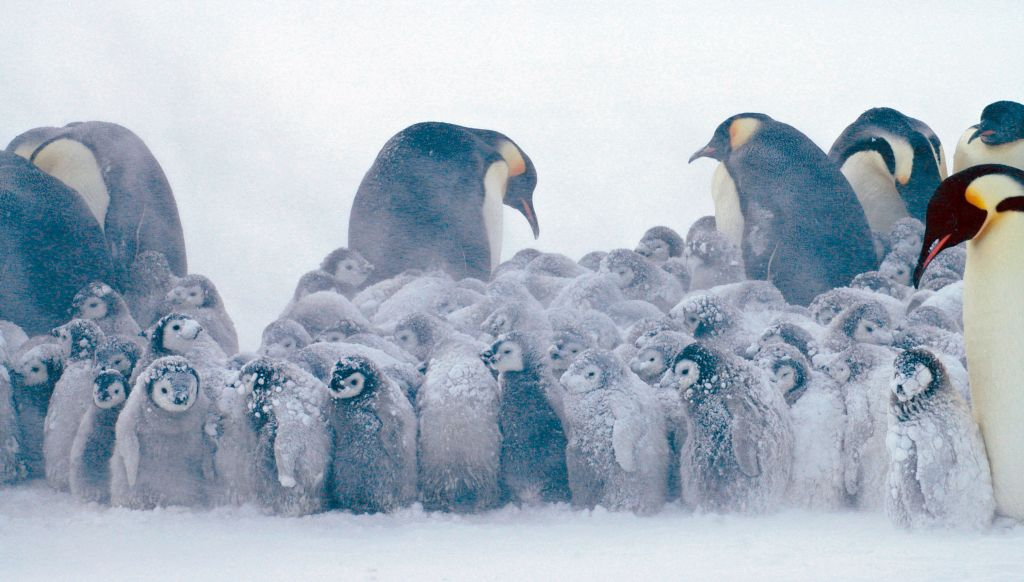
\includegraphics[scale=0.15, angle=5]{pics/bzip2penguin.jpg}
  \end{subfigure}\hfill
  \begin{subfigure}[b]{.45\linewidth}
  	\centering
  	\uncover<2>{
    \caption{lz4-Penguins}
    \label{fig:b}
    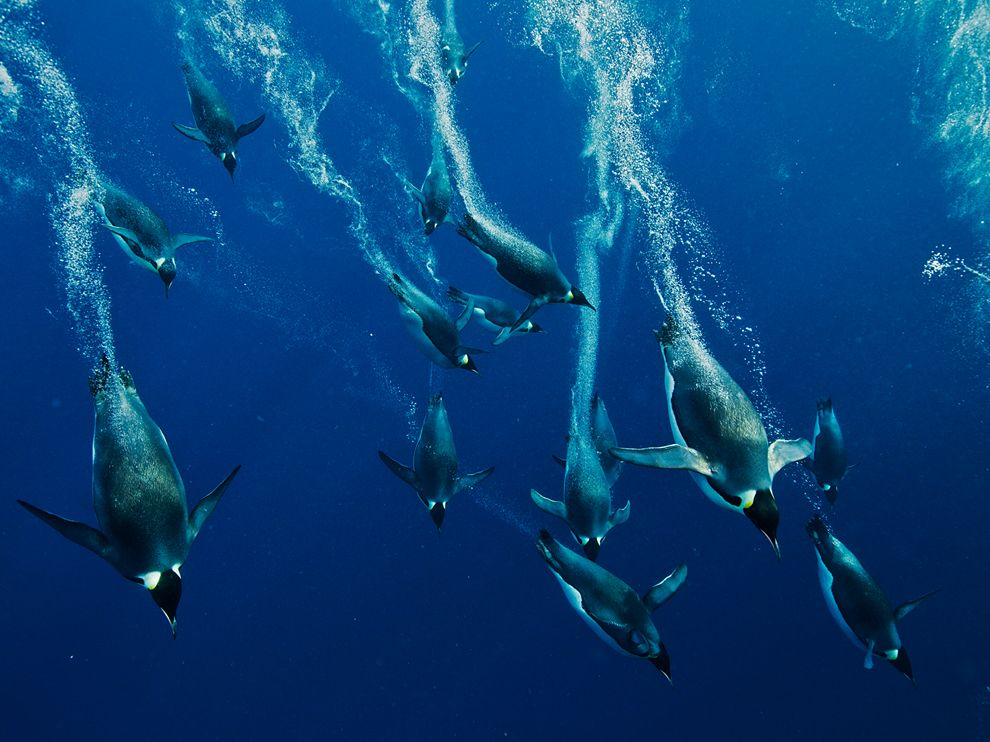
\includegraphics[scale=0.15, angle=-5]{pics/lz4pinguin.jpg}
    }
  \end{subfigure}
\end{figure}
\end{frame}


\begin{frame}{Summary}
	%TODO
\end{frame}

\end{document}